\documentclass{book}
\usepackage[a4paper,top=2.5cm,bottom=2.5cm,left=2.5cm,right=2.5cm]{geometry}
\usepackage{makeidx}
\usepackage{natbib}
\usepackage{graphicx}
\usepackage{multicol}
\usepackage{float}
\usepackage{listings}
\usepackage{color}
\usepackage{ifthen}
\usepackage[table]{xcolor}
\usepackage{textcomp}
\usepackage{alltt}
\usepackage{ifpdf}
\ifpdf
\usepackage[pdftex,
            pagebackref=true,
            colorlinks=true,
            linkcolor=blue,
            unicode
           ]{hyperref}
\else
\usepackage[ps2pdf,
            pagebackref=true,
            colorlinks=true,
            linkcolor=blue,
            unicode
           ]{hyperref}
\usepackage{pspicture}
\fi
\usepackage[utf8]{inputenc}
\usepackage{mathptmx}
\usepackage[scaled=.90]{helvet}
\usepackage{courier}
\usepackage{sectsty}
\usepackage{amssymb}
\usepackage[titles]{tocloft}
\usepackage{doxygen}
\lstset{language=C++,inputencoding=utf8,basicstyle=\footnotesize,breaklines=true,breakatwhitespace=true,tabsize=8,numbers=left }
\makeindex
\setcounter{tocdepth}{3}
\renewcommand{\footrulewidth}{0.4pt}
\renewcommand{\familydefault}{\sfdefault}
\hfuzz=15pt
\setlength{\emergencystretch}{15pt}
\hbadness=750
\tolerance=750
\begin{document}
\hypersetup{pageanchor=false,citecolor=blue}
\begin{titlepage}
\vspace*{7cm}
\begin{center}
{\Large Ether\-X\-Tag \\[1ex]\large 1 }\\
\vspace*{1cm}
{\large Generated by Doxygen 1.8.1.2}\\
\vspace*{0.5cm}
{\small Fri Oct 3 2014 12:38:24}\\
\end{center}
\end{titlepage}
\clearemptydoublepage
\pagenumbering{roman}
\tableofcontents
\clearemptydoublepage
\pagenumbering{arabic}
\hypersetup{pageanchor=true,citecolor=blue}
\chapter{Data Structure Index}
\section{Data Structures}
Here are the data structures with brief descriptions\-:\begin{DoxyCompactList}
\item\contentsline{section}{\hyperlink{structconnection__type__t}{connection\-\_\-type\-\_\-t} }{\pageref{structconnection__type__t}}{}
\item\contentsline{section}{\hyperlink{structdbg__cmd__packet}{dbg\-\_\-cmd\-\_\-packet} }{\pageref{structdbg__cmd__packet}}{}
\item\contentsline{section}{\hyperlink{structdbg__cmd__type__add__break}{dbg\-\_\-cmd\-\_\-type\-\_\-add\-\_\-break} }{\pageref{structdbg__cmd__type__add__break}}{}
\item\contentsline{section}{\hyperlink{structdbg__cmd__type__connect}{dbg\-\_\-cmd\-\_\-type\-\_\-connect} }{\pageref{structdbg__cmd__type__connect}}{}
\item\contentsline{section}{\hyperlink{structdbg__cmd__type__connect__xscope__channel}{dbg\-\_\-cmd\-\_\-type\-\_\-connect\-\_\-xscope\-\_\-channel} }{\pageref{structdbg__cmd__type__connect__xscope__channel}}{}
\item\contentsline{section}{\hyperlink{structdbg__cmd__type__continue}{dbg\-\_\-cmd\-\_\-type\-\_\-continue} }{\pageref{structdbg__cmd__type__continue}}{}
\item\contentsline{section}{\hyperlink{structdbg__cmd__type__disable__thread}{dbg\-\_\-cmd\-\_\-type\-\_\-disable\-\_\-thread} }{\pageref{structdbg__cmd__type__disable__thread}}{}
\item\contentsline{section}{\hyperlink{structdbg__cmd__type__disconnect}{dbg\-\_\-cmd\-\_\-type\-\_\-disconnect} }{\pageref{structdbg__cmd__type__disconnect}}{}
\item\contentsline{section}{\hyperlink{structdbg__cmd__type__enable__thread}{dbg\-\_\-cmd\-\_\-type\-\_\-enable\-\_\-thread} }{\pageref{structdbg__cmd__type__enable__thread}}{}
\item\contentsline{section}{\hyperlink{structdbg__cmd__type__firmware__reboot}{dbg\-\_\-cmd\-\_\-type\-\_\-firmware\-\_\-reboot} }{\pageref{structdbg__cmd__type__firmware__reboot}}{}
\item\contentsline{section}{\hyperlink{structdbg__cmd__type__firmware__version}{dbg\-\_\-cmd\-\_\-type\-\_\-firmware\-\_\-version} }{\pageref{structdbg__cmd__type__firmware__version}}{}
\item\contentsline{section}{\hyperlink{structdbg__cmd__type__get__chip__info}{dbg\-\_\-cmd\-\_\-type\-\_\-get\-\_\-chip\-\_\-info} }{\pageref{structdbg__cmd__type__get__chip__info}}{}
\item\contentsline{section}{\hyperlink{structdbg__cmd__type__get__core__state}{dbg\-\_\-cmd\-\_\-type\-\_\-get\-\_\-core\-\_\-state} }{\pageref{structdbg__cmd__type__get__core__state}}{}
\item\contentsline{section}{\hyperlink{structdbg__cmd__type__get__jtag__chain}{dbg\-\_\-cmd\-\_\-type\-\_\-get\-\_\-jtag\-\_\-chain} }{\pageref{structdbg__cmd__type__get__jtag__chain}}{}
\item\contentsline{section}{\hyperlink{structdbg__cmd__type__get__status}{dbg\-\_\-cmd\-\_\-type\-\_\-get\-\_\-status} }{\pageref{structdbg__cmd__type__get__status}}{}
\item\contentsline{section}{\hyperlink{structdbg__cmd__type__interrupt}{dbg\-\_\-cmd\-\_\-type\-\_\-interrupt} }{\pageref{structdbg__cmd__type__interrupt}}{}
\item\contentsline{section}{\hyperlink{structdbg__cmd__type__jtag__pc__sample}{dbg\-\_\-cmd\-\_\-type\-\_\-jtag\-\_\-pc\-\_\-sample} }{\pageref{structdbg__cmd__type__jtag__pc__sample}}{}
\item\contentsline{section}{\hyperlink{structdbg__cmd__type__jtag__pins}{dbg\-\_\-cmd\-\_\-type\-\_\-jtag\-\_\-pins} }{\pageref{structdbg__cmd__type__jtag__pins}}{}
\item\contentsline{section}{\hyperlink{structdbg__cmd__type__read__jtag__reg}{dbg\-\_\-cmd\-\_\-type\-\_\-read\-\_\-jtag\-\_\-reg} }{\pageref{structdbg__cmd__type__read__jtag__reg}}{}
\item\contentsline{section}{\hyperlink{structdbg__cmd__type__read__mem}{dbg\-\_\-cmd\-\_\-type\-\_\-read\-\_\-mem} }{\pageref{structdbg__cmd__type__read__mem}}{}
\item\contentsline{section}{\hyperlink{structdbg__cmd__type__read__obj}{dbg\-\_\-cmd\-\_\-type\-\_\-read\-\_\-obj} }{\pageref{structdbg__cmd__type__read__obj}}{}
\item\contentsline{section}{\hyperlink{structdbg__cmd__type__read__regs}{dbg\-\_\-cmd\-\_\-type\-\_\-read\-\_\-regs} }{\pageref{structdbg__cmd__type__read__regs}}{}
\item\contentsline{section}{\hyperlink{structdbg__cmd__type__remove__break}{dbg\-\_\-cmd\-\_\-type\-\_\-remove\-\_\-break} }{\pageref{structdbg__cmd__type__remove__break}}{}
\item\contentsline{section}{\hyperlink{structdbg__cmd__type__reset}{dbg\-\_\-cmd\-\_\-type\-\_\-reset} }{\pageref{structdbg__cmd__type__reset}}{}
\item\contentsline{section}{\hyperlink{structdbg__cmd__type__step}{dbg\-\_\-cmd\-\_\-type\-\_\-step} }{\pageref{structdbg__cmd__type__step}}{}
\item\contentsline{section}{\hyperlink{structdbg__cmd__type__upload__xscope__data}{dbg\-\_\-cmd\-\_\-type\-\_\-upload\-\_\-xscope\-\_\-data} }{\pageref{structdbg__cmd__type__upload__xscope__data}}{}
\item\contentsline{section}{\hyperlink{structdbg__cmd__type__write__jtag__reg}{dbg\-\_\-cmd\-\_\-type\-\_\-write\-\_\-jtag\-\_\-reg} }{\pageref{structdbg__cmd__type__write__jtag__reg}}{}
\item\contentsline{section}{\hyperlink{structdbg__cmd__type__write__mem}{dbg\-\_\-cmd\-\_\-type\-\_\-write\-\_\-mem} }{\pageref{structdbg__cmd__type__write__mem}}{}
\item\contentsline{section}{\hyperlink{structdbg__cmd__type__write__regs}{dbg\-\_\-cmd\-\_\-type\-\_\-write\-\_\-regs} }{\pageref{structdbg__cmd__type__write__regs}}{}
\item\contentsline{section}{\hyperlink{structdns__flags__t}{dns\-\_\-flags\-\_\-t} }{\pageref{structdns__flags__t}}{}
\item\contentsline{section}{\hyperlink{structdns__packet__header__t}{dns\-\_\-packet\-\_\-header\-\_\-t} \\*D\-N\-S Packet header }{\pageref{structdns__packet__header__t}}{}
\item\contentsline{section}{\hyperlink{structdns__packet__t}{dns\-\_\-packet\-\_\-t} \\*D\-N\-S Packet }{\pageref{structdns__packet__t}}{}
\item\contentsline{section}{\hyperlink{structjtag__response__t}{jtag\-\_\-response\-\_\-t} }{\pageref{structjtag__response__t}}{}
\item\contentsline{section}{\hyperlink{structpage__t}{page\-\_\-t} }{\pageref{structpage__t}}{}
\item\contentsline{section}{\hyperlink{structsystem__state__t}{system\-\_\-state\-\_\-t} \\*System state }{\pageref{structsystem__state__t}}{}
\end{DoxyCompactList}

\chapter{File Index}
\section{File List}
Here is a list of all files with brief descriptions\-:\begin{DoxyCompactList}
\item\contentsline{section}{Ether\-X\-Tag/src/\hyperlink{dbg__access_8c}{dbg\-\_\-access.\-c} }{\pageref{dbg__access_8c}}{}
\item\contentsline{section}{Ether\-X\-Tag/src/\hyperlink{dbg__access_8h}{dbg\-\_\-access.\-h} }{\pageref{dbg__access_8h}}{}
\item\contentsline{section}{Ether\-X\-Tag/src/\hyperlink{dbg__cmd_8h}{dbg\-\_\-cmd.\-h} }{\pageref{dbg__cmd_8h}}{}
\item\contentsline{section}{Ether\-X\-Tag/src/\hyperlink{dbg__interface_8cpp}{dbg\-\_\-interface.\-cpp} }{\pageref{dbg__interface_8cpp}}{}
\item\contentsline{section}{Ether\-X\-Tag/src/\hyperlink{ethernet__board__conf_8h}{ethernet\-\_\-board\-\_\-conf.\-h} }{\pageref{ethernet__board__conf_8h}}{}
\item\contentsline{section}{Ether\-X\-Tag/src/\hyperlink{mdns_8c}{mdns.\-c} }{\pageref{mdns_8c}}{}
\item\contentsline{section}{Ether\-X\-Tag/src/\hyperlink{mdns_8h}{mdns.\-h} }{\pageref{mdns_8h}}{}
\item\contentsline{section}{Ether\-X\-Tag/src/\hyperlink{state_8h}{state.\-h} }{\pageref{state_8h}}{}
\item\contentsline{section}{Ether\-X\-Tag/src/\hyperlink{tcp_8c}{tcp.\-c} }{\pageref{tcp_8c}}{}
\item\contentsline{section}{Ether\-X\-Tag/src/\hyperlink{tcp_8h}{tcp.\-h} }{\pageref{tcp_8h}}{}
\item\contentsline{section}{Ether\-X\-Tag/src/\hyperlink{udp_8c}{udp.\-c} }{\pageref{udp_8c}}{}
\item\contentsline{section}{Ether\-X\-Tag/src/\hyperlink{udp_8h}{udp.\-h} }{\pageref{udp_8h}}{}
\item\contentsline{section}{Ether\-X\-Tag/src/\hyperlink{web__service_8c}{web\-\_\-service.\-c} }{\pageref{web__service_8c}}{}
\item\contentsline{section}{Ether\-X\-Tag/src/\hyperlink{web__service_8h}{web\-\_\-service.\-h} }{\pageref{web__service_8h}}{}
\end{DoxyCompactList}

\chapter{Data Structure Documentation}
\hypertarget{structconnection__type__t}{\section{connection\-\_\-type\-\_\-t Struct Reference}
\label{structconnection__type__t}\index{connection\-\_\-type\-\_\-t@{connection\-\_\-type\-\_\-t}}
}
\subsection*{Data Fields}
\begin{DoxyCompactItemize}
\item 
int \hyperlink{structconnection__type__t_aa5805c5e936174e5092bf7a5b78e7e64}{active}
\item 
int \hyperlink{structconnection__type__t_a11be20eefd18549b1a7b6b2f1d7dca52}{conn\-\_\-id}
\item 
char $\ast$ \hyperlink{structconnection__type__t_a2d9df43d157669dbcc90879f8ee350ff}{dptr}
\item 
int \hyperlink{structconnection__type__t_a142672f9be33d53e1ecf96db7104a396}{dlen}
\item 
char $\ast$ \hyperlink{structconnection__type__t_a3950706000f1bfe0b448d9b632624521}{prev\-\_\-dptr}
\end{DoxyCompactItemize}


\subsection{Detailed Description}


Definition at line 16 of file tcp.\-c.



\subsection{Field Documentation}
\hypertarget{structconnection__type__t_aa5805c5e936174e5092bf7a5b78e7e64}{\index{connection\-\_\-type\-\_\-t@{connection\-\_\-type\-\_\-t}!active@{active}}
\index{active@{active}!connection_type_t@{connection\-\_\-type\-\_\-t}}
\subsubsection[{active}]{\setlength{\rightskip}{0pt plus 5cm}int active}}\label{structconnection__type__t_aa5805c5e936174e5092bf7a5b78e7e64}


Definition at line 17 of file tcp.\-c.

\hypertarget{structconnection__type__t_a11be20eefd18549b1a7b6b2f1d7dca52}{\index{connection\-\_\-type\-\_\-t@{connection\-\_\-type\-\_\-t}!conn\-\_\-id@{conn\-\_\-id}}
\index{conn\-\_\-id@{conn\-\_\-id}!connection_type_t@{connection\-\_\-type\-\_\-t}}
\subsubsection[{conn\-\_\-id}]{\setlength{\rightskip}{0pt plus 5cm}int conn\-\_\-id}}\label{structconnection__type__t_a11be20eefd18549b1a7b6b2f1d7dca52}


Definition at line 19 of file tcp.\-c.

\hypertarget{structconnection__type__t_a142672f9be33d53e1ecf96db7104a396}{\index{connection\-\_\-type\-\_\-t@{connection\-\_\-type\-\_\-t}!dlen@{dlen}}
\index{dlen@{dlen}!connection_type_t@{connection\-\_\-type\-\_\-t}}
\subsubsection[{dlen}]{\setlength{\rightskip}{0pt plus 5cm}int dlen}}\label{structconnection__type__t_a142672f9be33d53e1ecf96db7104a396}


Definition at line 21 of file tcp.\-c.

\hypertarget{structconnection__type__t_a2d9df43d157669dbcc90879f8ee350ff}{\index{connection\-\_\-type\-\_\-t@{connection\-\_\-type\-\_\-t}!dptr@{dptr}}
\index{dptr@{dptr}!connection_type_t@{connection\-\_\-type\-\_\-t}}
\subsubsection[{dptr}]{\setlength{\rightskip}{0pt plus 5cm}char $\ast$ dptr}}\label{structconnection__type__t_a2d9df43d157669dbcc90879f8ee350ff}


Definition at line 20 of file tcp.\-c.

\hypertarget{structconnection__type__t_a3950706000f1bfe0b448d9b632624521}{\index{connection\-\_\-type\-\_\-t@{connection\-\_\-type\-\_\-t}!prev\-\_\-dptr@{prev\-\_\-dptr}}
\index{prev\-\_\-dptr@{prev\-\_\-dptr}!connection_type_t@{connection\-\_\-type\-\_\-t}}
\subsubsection[{prev\-\_\-dptr}]{\setlength{\rightskip}{0pt plus 5cm}char $\ast$ prev\-\_\-dptr}}\label{structconnection__type__t_a3950706000f1bfe0b448d9b632624521}


Definition at line 22 of file tcp.\-c.



The documentation for this struct was generated from the following files\-:\begin{DoxyCompactItemize}
\item 
Ether\-X\-Tag/src/\hyperlink{tcp_8c}{tcp.\-c}\item 
Ether\-X\-Tag/src/\hyperlink{udp_8c}{udp.\-c}\end{DoxyCompactItemize}

\hypertarget{structdbg__cmd__packet}{\section{dbg\-\_\-cmd\-\_\-packet Struct Reference}
\label{structdbg__cmd__packet}\index{dbg\-\_\-cmd\-\_\-packet@{dbg\-\_\-cmd\-\_\-packet}}
}


{\ttfamily \#include $<$dbg\-\_\-cmd.\-h$>$}

\subsection*{Data Fields}
\begin{DoxyCompactItemize}
\item 
enum \hyperlink{dbg__cmd_8h_a921a01d6be6d3bf1d52a1713a55b186d}{dbg\-\_\-cmd\-\_\-type} \hyperlink{structdbg__cmd__packet_a1e4ce97c93b772bbbacf726804cb1dd1}{type}
\item 
unsigned int \hyperlink{structdbg__cmd__packet_a3e301c82072246baef805fc5c0e3fd9a}{data} \mbox{[}\hyperlink{dbg__cmd_8h_abe6cfb003699e267c6bb15e549e269a4}{M\-A\-X\-\_\-\-D\-B\-G\-\_\-\-C\-M\-D\-\_\-\-L\-E\-N}-\/1\mbox{]}
\end{DoxyCompactItemize}


\subsection{Detailed Description}


Definition at line 72 of file dbg\-\_\-cmd.\-h.



\subsection{Field Documentation}
\hypertarget{structdbg__cmd__packet_a3e301c82072246baef805fc5c0e3fd9a}{\index{dbg\-\_\-cmd\-\_\-packet@{dbg\-\_\-cmd\-\_\-packet}!data@{data}}
\index{data@{data}!dbg_cmd_packet@{dbg\-\_\-cmd\-\_\-packet}}
\subsubsection[{data}]{\setlength{\rightskip}{0pt plus 5cm}unsigned int data\mbox{[}{\bf M\-A\-X\-\_\-\-D\-B\-G\-\_\-\-C\-M\-D\-\_\-\-L\-E\-N}-\/1\mbox{]}}}\label{structdbg__cmd__packet_a3e301c82072246baef805fc5c0e3fd9a}


Definition at line 74 of file dbg\-\_\-cmd.\-h.

\hypertarget{structdbg__cmd__packet_a1e4ce97c93b772bbbacf726804cb1dd1}{\index{dbg\-\_\-cmd\-\_\-packet@{dbg\-\_\-cmd\-\_\-packet}!type@{type}}
\index{type@{type}!dbg_cmd_packet@{dbg\-\_\-cmd\-\_\-packet}}
\subsubsection[{type}]{\setlength{\rightskip}{0pt plus 5cm}enum {\bf dbg\-\_\-cmd\-\_\-type} type}}\label{structdbg__cmd__packet_a1e4ce97c93b772bbbacf726804cb1dd1}


Definition at line 73 of file dbg\-\_\-cmd.\-h.



The documentation for this struct was generated from the following file\-:\begin{DoxyCompactItemize}
\item 
Ether\-X\-Tag/src/\hyperlink{dbg__cmd_8h}{dbg\-\_\-cmd.\-h}\end{DoxyCompactItemize}

\hypertarget{structdbg__cmd__type__add__break}{\section{dbg\-\_\-cmd\-\_\-type\-\_\-add\-\_\-break Struct Reference}
\label{structdbg__cmd__type__add__break}\index{dbg\-\_\-cmd\-\_\-type\-\_\-add\-\_\-break@{dbg\-\_\-cmd\-\_\-type\-\_\-add\-\_\-break}}
}


{\ttfamily \#include $<$dbg\-\_\-cmd.\-h$>$}

\subsection*{Data Fields}
\begin{DoxyCompactItemize}
\item 
unsigned int \hyperlink{structdbg__cmd__type__add__break_a78357326dd562d441c3c73f5676ac638}{xcore}
\item 
unsigned int \hyperlink{structdbg__cmd__type__add__break_a13f572e7828e1694c6f9c9c78bf7d8f5}{thread}
\item 
unsigned int \hyperlink{structdbg__cmd__type__add__break_a2f55ff1f6cd45ca1b6431493ab5614eb}{address}
\item 
unsigned int \hyperlink{structdbg__cmd__type__add__break_ac8d42bcd4a44e078047ccd7291059238}{length}
\item 
unsigned int \hyperlink{structdbg__cmd__type__add__break_a4bfea42429249a1f65204f0c0f34704a}{type}
\item 
unsigned int \hyperlink{structdbg__cmd__type__add__break_ab91dff01c2f12e354ddb4becbe93f063}{data} \mbox{[}\hyperlink{dbg__cmd_8h_a4552ec15033c8a68870cdf80eda5470c}{M\-A\-X\-\_\-\-D\-B\-G\-\_\-\-C\-M\-D\-\_\-\-D\-A\-T\-A\-\_\-\-L\-E\-N}-\/5\mbox{]}
\end{DoxyCompactItemize}


\subsection{Detailed Description}


Definition at line 165 of file dbg\-\_\-cmd.\-h.



\subsection{Field Documentation}
\hypertarget{structdbg__cmd__type__add__break_a2f55ff1f6cd45ca1b6431493ab5614eb}{\index{dbg\-\_\-cmd\-\_\-type\-\_\-add\-\_\-break@{dbg\-\_\-cmd\-\_\-type\-\_\-add\-\_\-break}!address@{address}}
\index{address@{address}!dbg_cmd_type_add_break@{dbg\-\_\-cmd\-\_\-type\-\_\-add\-\_\-break}}
\subsubsection[{address}]{\setlength{\rightskip}{0pt plus 5cm}unsigned int address}}\label{structdbg__cmd__type__add__break_a2f55ff1f6cd45ca1b6431493ab5614eb}


Definition at line 168 of file dbg\-\_\-cmd.\-h.

\hypertarget{structdbg__cmd__type__add__break_ab91dff01c2f12e354ddb4becbe93f063}{\index{dbg\-\_\-cmd\-\_\-type\-\_\-add\-\_\-break@{dbg\-\_\-cmd\-\_\-type\-\_\-add\-\_\-break}!data@{data}}
\index{data@{data}!dbg_cmd_type_add_break@{dbg\-\_\-cmd\-\_\-type\-\_\-add\-\_\-break}}
\subsubsection[{data}]{\setlength{\rightskip}{0pt plus 5cm}unsigned int data\mbox{[}{\bf M\-A\-X\-\_\-\-D\-B\-G\-\_\-\-C\-M\-D\-\_\-\-D\-A\-T\-A\-\_\-\-L\-E\-N}-\/5\mbox{]}}}\label{structdbg__cmd__type__add__break_ab91dff01c2f12e354ddb4becbe93f063}


Definition at line 171 of file dbg\-\_\-cmd.\-h.

\hypertarget{structdbg__cmd__type__add__break_ac8d42bcd4a44e078047ccd7291059238}{\index{dbg\-\_\-cmd\-\_\-type\-\_\-add\-\_\-break@{dbg\-\_\-cmd\-\_\-type\-\_\-add\-\_\-break}!length@{length}}
\index{length@{length}!dbg_cmd_type_add_break@{dbg\-\_\-cmd\-\_\-type\-\_\-add\-\_\-break}}
\subsubsection[{length}]{\setlength{\rightskip}{0pt plus 5cm}unsigned int length}}\label{structdbg__cmd__type__add__break_ac8d42bcd4a44e078047ccd7291059238}


Definition at line 169 of file dbg\-\_\-cmd.\-h.

\hypertarget{structdbg__cmd__type__add__break_a13f572e7828e1694c6f9c9c78bf7d8f5}{\index{dbg\-\_\-cmd\-\_\-type\-\_\-add\-\_\-break@{dbg\-\_\-cmd\-\_\-type\-\_\-add\-\_\-break}!thread@{thread}}
\index{thread@{thread}!dbg_cmd_type_add_break@{dbg\-\_\-cmd\-\_\-type\-\_\-add\-\_\-break}}
\subsubsection[{thread}]{\setlength{\rightskip}{0pt plus 5cm}unsigned int thread}}\label{structdbg__cmd__type__add__break_a13f572e7828e1694c6f9c9c78bf7d8f5}


Definition at line 167 of file dbg\-\_\-cmd.\-h.

\hypertarget{structdbg__cmd__type__add__break_a4bfea42429249a1f65204f0c0f34704a}{\index{dbg\-\_\-cmd\-\_\-type\-\_\-add\-\_\-break@{dbg\-\_\-cmd\-\_\-type\-\_\-add\-\_\-break}!type@{type}}
\index{type@{type}!dbg_cmd_type_add_break@{dbg\-\_\-cmd\-\_\-type\-\_\-add\-\_\-break}}
\subsubsection[{type}]{\setlength{\rightskip}{0pt plus 5cm}unsigned int type}}\label{structdbg__cmd__type__add__break_a4bfea42429249a1f65204f0c0f34704a}


Definition at line 170 of file dbg\-\_\-cmd.\-h.

\hypertarget{structdbg__cmd__type__add__break_a78357326dd562d441c3c73f5676ac638}{\index{dbg\-\_\-cmd\-\_\-type\-\_\-add\-\_\-break@{dbg\-\_\-cmd\-\_\-type\-\_\-add\-\_\-break}!xcore@{xcore}}
\index{xcore@{xcore}!dbg_cmd_type_add_break@{dbg\-\_\-cmd\-\_\-type\-\_\-add\-\_\-break}}
\subsubsection[{xcore}]{\setlength{\rightskip}{0pt plus 5cm}unsigned int xcore}}\label{structdbg__cmd__type__add__break_a78357326dd562d441c3c73f5676ac638}


Definition at line 166 of file dbg\-\_\-cmd.\-h.



The documentation for this struct was generated from the following file\-:\begin{DoxyCompactItemize}
\item 
Ether\-X\-Tag/src/\hyperlink{dbg__cmd_8h}{dbg\-\_\-cmd.\-h}\end{DoxyCompactItemize}

\hypertarget{structdbg__cmd__type__connect}{\section{dbg\-\_\-cmd\-\_\-type\-\_\-connect Struct Reference}
\label{structdbg__cmd__type__connect}\index{dbg\-\_\-cmd\-\_\-type\-\_\-connect@{dbg\-\_\-cmd\-\_\-type\-\_\-connect}}
}


{\ttfamily \#include $<$dbg\-\_\-cmd.\-h$>$}

\subsection*{Data Fields}
\begin{DoxyCompactItemize}
\item 
int \hyperlink{structdbg__cmd__type__connect_a46e35e0c4106e70b82f3a8961e735ab2}{jtag\-\_\-speed}
\item 
unsigned int \hyperlink{structdbg__cmd__type__connect_a641ec70530418c7d2b8aef7e638d4a71}{debug\-\_\-enabled}
\item 
unsigned int \hyperlink{structdbg__cmd__type__connect_aac2104a47b226a8d04018b775a3b9fd5}{jtag\-\_\-devs\-\_\-pre}
\item 
unsigned int \hyperlink{structdbg__cmd__type__connect_a6f238ba20b72ab6f00f7f9a399e2fa68}{jtag\-\_\-bits\-\_\-pre}
\item 
unsigned int \hyperlink{structdbg__cmd__type__connect_a90dd173c303603d84b29e370867f31d9}{jtag\-\_\-devs\-\_\-post}
\item 
unsigned int \hyperlink{structdbg__cmd__type__connect_a78a4d89034acb5a7f350517ca435bcf4}{jtag\-\_\-bits\-\_\-post}
\item 
unsigned int \hyperlink{structdbg__cmd__type__connect_afab09200baf8322f1d8e65fc4669c32c}{jtag\-\_\-max\-\_\-speed}
\item 
unsigned int \hyperlink{structdbg__cmd__type__connect_ac3fe8764cbd797e43e0dc2c4977659b5}{enable\-\_\-digital\-\_\-scope}
\item 
unsigned int \hyperlink{structdbg__cmd__type__connect_a8f69251f33a0e0c36839fa771ec1993e}{enable\-\_\-analog\-\_\-scope}
\item 
unsigned int \hyperlink{structdbg__cmd__type__connect_ae7632a28dd6ad1e333af08fca1d0f6cb}{data} \mbox{[}\hyperlink{dbg__cmd_8h_a4552ec15033c8a68870cdf80eda5470c}{M\-A\-X\-\_\-\-D\-B\-G\-\_\-\-C\-M\-D\-\_\-\-D\-A\-T\-A\-\_\-\-L\-E\-N}-\/9\mbox{]}
\end{DoxyCompactItemize}


\subsection{Detailed Description}


Definition at line 77 of file dbg\-\_\-cmd.\-h.



\subsection{Field Documentation}
\hypertarget{structdbg__cmd__type__connect_ae7632a28dd6ad1e333af08fca1d0f6cb}{\index{dbg\-\_\-cmd\-\_\-type\-\_\-connect@{dbg\-\_\-cmd\-\_\-type\-\_\-connect}!data@{data}}
\index{data@{data}!dbg_cmd_type_connect@{dbg\-\_\-cmd\-\_\-type\-\_\-connect}}
\subsubsection[{data}]{\setlength{\rightskip}{0pt plus 5cm}unsigned int data\mbox{[}{\bf M\-A\-X\-\_\-\-D\-B\-G\-\_\-\-C\-M\-D\-\_\-\-D\-A\-T\-A\-\_\-\-L\-E\-N}-\/9\mbox{]}}}\label{structdbg__cmd__type__connect_ae7632a28dd6ad1e333af08fca1d0f6cb}


Definition at line 87 of file dbg\-\_\-cmd.\-h.

\hypertarget{structdbg__cmd__type__connect_a641ec70530418c7d2b8aef7e638d4a71}{\index{dbg\-\_\-cmd\-\_\-type\-\_\-connect@{dbg\-\_\-cmd\-\_\-type\-\_\-connect}!debug\-\_\-enabled@{debug\-\_\-enabled}}
\index{debug\-\_\-enabled@{debug\-\_\-enabled}!dbg_cmd_type_connect@{dbg\-\_\-cmd\-\_\-type\-\_\-connect}}
\subsubsection[{debug\-\_\-enabled}]{\setlength{\rightskip}{0pt plus 5cm}unsigned int debug\-\_\-enabled}}\label{structdbg__cmd__type__connect_a641ec70530418c7d2b8aef7e638d4a71}


Definition at line 79 of file dbg\-\_\-cmd.\-h.

\hypertarget{structdbg__cmd__type__connect_a8f69251f33a0e0c36839fa771ec1993e}{\index{dbg\-\_\-cmd\-\_\-type\-\_\-connect@{dbg\-\_\-cmd\-\_\-type\-\_\-connect}!enable\-\_\-analog\-\_\-scope@{enable\-\_\-analog\-\_\-scope}}
\index{enable\-\_\-analog\-\_\-scope@{enable\-\_\-analog\-\_\-scope}!dbg_cmd_type_connect@{dbg\-\_\-cmd\-\_\-type\-\_\-connect}}
\subsubsection[{enable\-\_\-analog\-\_\-scope}]{\setlength{\rightskip}{0pt plus 5cm}unsigned int enable\-\_\-analog\-\_\-scope}}\label{structdbg__cmd__type__connect_a8f69251f33a0e0c36839fa771ec1993e}


Definition at line 86 of file dbg\-\_\-cmd.\-h.

\hypertarget{structdbg__cmd__type__connect_ac3fe8764cbd797e43e0dc2c4977659b5}{\index{dbg\-\_\-cmd\-\_\-type\-\_\-connect@{dbg\-\_\-cmd\-\_\-type\-\_\-connect}!enable\-\_\-digital\-\_\-scope@{enable\-\_\-digital\-\_\-scope}}
\index{enable\-\_\-digital\-\_\-scope@{enable\-\_\-digital\-\_\-scope}!dbg_cmd_type_connect@{dbg\-\_\-cmd\-\_\-type\-\_\-connect}}
\subsubsection[{enable\-\_\-digital\-\_\-scope}]{\setlength{\rightskip}{0pt plus 5cm}unsigned int enable\-\_\-digital\-\_\-scope}}\label{structdbg__cmd__type__connect_ac3fe8764cbd797e43e0dc2c4977659b5}


Definition at line 85 of file dbg\-\_\-cmd.\-h.

\hypertarget{structdbg__cmd__type__connect_a78a4d89034acb5a7f350517ca435bcf4}{\index{dbg\-\_\-cmd\-\_\-type\-\_\-connect@{dbg\-\_\-cmd\-\_\-type\-\_\-connect}!jtag\-\_\-bits\-\_\-post@{jtag\-\_\-bits\-\_\-post}}
\index{jtag\-\_\-bits\-\_\-post@{jtag\-\_\-bits\-\_\-post}!dbg_cmd_type_connect@{dbg\-\_\-cmd\-\_\-type\-\_\-connect}}
\subsubsection[{jtag\-\_\-bits\-\_\-post}]{\setlength{\rightskip}{0pt plus 5cm}unsigned int jtag\-\_\-bits\-\_\-post}}\label{structdbg__cmd__type__connect_a78a4d89034acb5a7f350517ca435bcf4}


Definition at line 83 of file dbg\-\_\-cmd.\-h.

\hypertarget{structdbg__cmd__type__connect_a6f238ba20b72ab6f00f7f9a399e2fa68}{\index{dbg\-\_\-cmd\-\_\-type\-\_\-connect@{dbg\-\_\-cmd\-\_\-type\-\_\-connect}!jtag\-\_\-bits\-\_\-pre@{jtag\-\_\-bits\-\_\-pre}}
\index{jtag\-\_\-bits\-\_\-pre@{jtag\-\_\-bits\-\_\-pre}!dbg_cmd_type_connect@{dbg\-\_\-cmd\-\_\-type\-\_\-connect}}
\subsubsection[{jtag\-\_\-bits\-\_\-pre}]{\setlength{\rightskip}{0pt plus 5cm}unsigned int jtag\-\_\-bits\-\_\-pre}}\label{structdbg__cmd__type__connect_a6f238ba20b72ab6f00f7f9a399e2fa68}


Definition at line 81 of file dbg\-\_\-cmd.\-h.

\hypertarget{structdbg__cmd__type__connect_a90dd173c303603d84b29e370867f31d9}{\index{dbg\-\_\-cmd\-\_\-type\-\_\-connect@{dbg\-\_\-cmd\-\_\-type\-\_\-connect}!jtag\-\_\-devs\-\_\-post@{jtag\-\_\-devs\-\_\-post}}
\index{jtag\-\_\-devs\-\_\-post@{jtag\-\_\-devs\-\_\-post}!dbg_cmd_type_connect@{dbg\-\_\-cmd\-\_\-type\-\_\-connect}}
\subsubsection[{jtag\-\_\-devs\-\_\-post}]{\setlength{\rightskip}{0pt plus 5cm}unsigned int jtag\-\_\-devs\-\_\-post}}\label{structdbg__cmd__type__connect_a90dd173c303603d84b29e370867f31d9}


Definition at line 82 of file dbg\-\_\-cmd.\-h.

\hypertarget{structdbg__cmd__type__connect_aac2104a47b226a8d04018b775a3b9fd5}{\index{dbg\-\_\-cmd\-\_\-type\-\_\-connect@{dbg\-\_\-cmd\-\_\-type\-\_\-connect}!jtag\-\_\-devs\-\_\-pre@{jtag\-\_\-devs\-\_\-pre}}
\index{jtag\-\_\-devs\-\_\-pre@{jtag\-\_\-devs\-\_\-pre}!dbg_cmd_type_connect@{dbg\-\_\-cmd\-\_\-type\-\_\-connect}}
\subsubsection[{jtag\-\_\-devs\-\_\-pre}]{\setlength{\rightskip}{0pt plus 5cm}unsigned int jtag\-\_\-devs\-\_\-pre}}\label{structdbg__cmd__type__connect_aac2104a47b226a8d04018b775a3b9fd5}


Definition at line 80 of file dbg\-\_\-cmd.\-h.

\hypertarget{structdbg__cmd__type__connect_afab09200baf8322f1d8e65fc4669c32c}{\index{dbg\-\_\-cmd\-\_\-type\-\_\-connect@{dbg\-\_\-cmd\-\_\-type\-\_\-connect}!jtag\-\_\-max\-\_\-speed@{jtag\-\_\-max\-\_\-speed}}
\index{jtag\-\_\-max\-\_\-speed@{jtag\-\_\-max\-\_\-speed}!dbg_cmd_type_connect@{dbg\-\_\-cmd\-\_\-type\-\_\-connect}}
\subsubsection[{jtag\-\_\-max\-\_\-speed}]{\setlength{\rightskip}{0pt plus 5cm}unsigned int jtag\-\_\-max\-\_\-speed}}\label{structdbg__cmd__type__connect_afab09200baf8322f1d8e65fc4669c32c}


Definition at line 84 of file dbg\-\_\-cmd.\-h.

\hypertarget{structdbg__cmd__type__connect_a46e35e0c4106e70b82f3a8961e735ab2}{\index{dbg\-\_\-cmd\-\_\-type\-\_\-connect@{dbg\-\_\-cmd\-\_\-type\-\_\-connect}!jtag\-\_\-speed@{jtag\-\_\-speed}}
\index{jtag\-\_\-speed@{jtag\-\_\-speed}!dbg_cmd_type_connect@{dbg\-\_\-cmd\-\_\-type\-\_\-connect}}
\subsubsection[{jtag\-\_\-speed}]{\setlength{\rightskip}{0pt plus 5cm}int jtag\-\_\-speed}}\label{structdbg__cmd__type__connect_a46e35e0c4106e70b82f3a8961e735ab2}


Definition at line 78 of file dbg\-\_\-cmd.\-h.



The documentation for this struct was generated from the following file\-:\begin{DoxyCompactItemize}
\item 
Ether\-X\-Tag/src/\hyperlink{dbg__cmd_8h}{dbg\-\_\-cmd.\-h}\end{DoxyCompactItemize}

\hypertarget{structdbg__cmd__type__connect__xscope__channel}{\section{dbg\-\_\-cmd\-\_\-type\-\_\-connect\-\_\-xscope\-\_\-channel Struct Reference}
\label{structdbg__cmd__type__connect__xscope__channel}\index{dbg\-\_\-cmd\-\_\-type\-\_\-connect\-\_\-xscope\-\_\-channel@{dbg\-\_\-cmd\-\_\-type\-\_\-connect\-\_\-xscope\-\_\-channel}}
}


{\ttfamily \#include $<$dbg\-\_\-cmd.\-h$>$}

\subsection*{Data Fields}
\begin{DoxyCompactItemize}
\item 
unsigned int \hyperlink{structdbg__cmd__type__connect__xscope__channel_adb8779baf4a10ba8f92de8832641dff0}{channel\-End}
\item 
unsigned int \hyperlink{structdbg__cmd__type__connect__xscope__channel_abceed6826af53b88f4cc936fac1716f0}{data} \mbox{[}\hyperlink{dbg__cmd_8h_a4552ec15033c8a68870cdf80eda5470c}{M\-A\-X\-\_\-\-D\-B\-G\-\_\-\-C\-M\-D\-\_\-\-D\-A\-T\-A\-\_\-\-L\-E\-N}-\/1\mbox{]}
\end{DoxyCompactItemize}


\subsection{Detailed Description}


Definition at line 230 of file dbg\-\_\-cmd.\-h.



\subsection{Field Documentation}
\hypertarget{structdbg__cmd__type__connect__xscope__channel_adb8779baf4a10ba8f92de8832641dff0}{\index{dbg\-\_\-cmd\-\_\-type\-\_\-connect\-\_\-xscope\-\_\-channel@{dbg\-\_\-cmd\-\_\-type\-\_\-connect\-\_\-xscope\-\_\-channel}!channel\-End@{channel\-End}}
\index{channel\-End@{channel\-End}!dbg_cmd_type_connect_xscope_channel@{dbg\-\_\-cmd\-\_\-type\-\_\-connect\-\_\-xscope\-\_\-channel}}
\subsubsection[{channel\-End}]{\setlength{\rightskip}{0pt plus 5cm}unsigned int channel\-End}}\label{structdbg__cmd__type__connect__xscope__channel_adb8779baf4a10ba8f92de8832641dff0}


Definition at line 231 of file dbg\-\_\-cmd.\-h.

\hypertarget{structdbg__cmd__type__connect__xscope__channel_abceed6826af53b88f4cc936fac1716f0}{\index{dbg\-\_\-cmd\-\_\-type\-\_\-connect\-\_\-xscope\-\_\-channel@{dbg\-\_\-cmd\-\_\-type\-\_\-connect\-\_\-xscope\-\_\-channel}!data@{data}}
\index{data@{data}!dbg_cmd_type_connect_xscope_channel@{dbg\-\_\-cmd\-\_\-type\-\_\-connect\-\_\-xscope\-\_\-channel}}
\subsubsection[{data}]{\setlength{\rightskip}{0pt plus 5cm}unsigned int data\mbox{[}{\bf M\-A\-X\-\_\-\-D\-B\-G\-\_\-\-C\-M\-D\-\_\-\-D\-A\-T\-A\-\_\-\-L\-E\-N}-\/1\mbox{]}}}\label{structdbg__cmd__type__connect__xscope__channel_abceed6826af53b88f4cc936fac1716f0}


Definition at line 232 of file dbg\-\_\-cmd.\-h.



The documentation for this struct was generated from the following file\-:\begin{DoxyCompactItemize}
\item 
Ether\-X\-Tag/src/\hyperlink{dbg__cmd_8h}{dbg\-\_\-cmd.\-h}\end{DoxyCompactItemize}

\hypertarget{structdbg__cmd__type__continue}{\section{dbg\-\_\-cmd\-\_\-type\-\_\-continue Struct Reference}
\label{structdbg__cmd__type__continue}\index{dbg\-\_\-cmd\-\_\-type\-\_\-continue@{dbg\-\_\-cmd\-\_\-type\-\_\-continue}}
}


{\ttfamily \#include $<$dbg\-\_\-cmd.\-h$>$}

\subsection*{Data Fields}
\begin{DoxyCompactItemize}
\item 
unsigned int \hyperlink{structdbg__cmd__type__continue_a78357326dd562d441c3c73f5676ac638}{xcore}
\item 
unsigned int \hyperlink{structdbg__cmd__type__continue_abceed6826af53b88f4cc936fac1716f0}{data} \mbox{[}\hyperlink{dbg__cmd_8h_a4552ec15033c8a68870cdf80eda5470c}{M\-A\-X\-\_\-\-D\-B\-G\-\_\-\-C\-M\-D\-\_\-\-D\-A\-T\-A\-\_\-\-L\-E\-N}-\/1\mbox{]}
\end{DoxyCompactItemize}


\subsection{Detailed Description}


Definition at line 153 of file dbg\-\_\-cmd.\-h.



\subsection{Field Documentation}
\hypertarget{structdbg__cmd__type__continue_abceed6826af53b88f4cc936fac1716f0}{\index{dbg\-\_\-cmd\-\_\-type\-\_\-continue@{dbg\-\_\-cmd\-\_\-type\-\_\-continue}!data@{data}}
\index{data@{data}!dbg_cmd_type_continue@{dbg\-\_\-cmd\-\_\-type\-\_\-continue}}
\subsubsection[{data}]{\setlength{\rightskip}{0pt plus 5cm}unsigned int data\mbox{[}{\bf M\-A\-X\-\_\-\-D\-B\-G\-\_\-\-C\-M\-D\-\_\-\-D\-A\-T\-A\-\_\-\-L\-E\-N}-\/1\mbox{]}}}\label{structdbg__cmd__type__continue_abceed6826af53b88f4cc936fac1716f0}


Definition at line 155 of file dbg\-\_\-cmd.\-h.

\hypertarget{structdbg__cmd__type__continue_a78357326dd562d441c3c73f5676ac638}{\index{dbg\-\_\-cmd\-\_\-type\-\_\-continue@{dbg\-\_\-cmd\-\_\-type\-\_\-continue}!xcore@{xcore}}
\index{xcore@{xcore}!dbg_cmd_type_continue@{dbg\-\_\-cmd\-\_\-type\-\_\-continue}}
\subsubsection[{xcore}]{\setlength{\rightskip}{0pt plus 5cm}unsigned int xcore}}\label{structdbg__cmd__type__continue_a78357326dd562d441c3c73f5676ac638}


Definition at line 154 of file dbg\-\_\-cmd.\-h.



The documentation for this struct was generated from the following file\-:\begin{DoxyCompactItemize}
\item 
Ether\-X\-Tag/src/\hyperlink{dbg__cmd_8h}{dbg\-\_\-cmd.\-h}\end{DoxyCompactItemize}

\hypertarget{structdbg__cmd__type__disable__thread}{\section{dbg\-\_\-cmd\-\_\-type\-\_\-disable\-\_\-thread Struct Reference}
\label{structdbg__cmd__type__disable__thread}\index{dbg\-\_\-cmd\-\_\-type\-\_\-disable\-\_\-thread@{dbg\-\_\-cmd\-\_\-type\-\_\-disable\-\_\-thread}}
}


{\ttfamily \#include $<$dbg\-\_\-cmd.\-h$>$}

\subsection*{Data Fields}
\begin{DoxyCompactItemize}
\item 
unsigned int \hyperlink{structdbg__cmd__type__disable__thread_a78357326dd562d441c3c73f5676ac638}{xcore}
\item 
unsigned int \hyperlink{structdbg__cmd__type__disable__thread_abceed6826af53b88f4cc936fac1716f0}{data} \mbox{[}\hyperlink{dbg__cmd_8h_a4552ec15033c8a68870cdf80eda5470c}{M\-A\-X\-\_\-\-D\-B\-G\-\_\-\-C\-M\-D\-\_\-\-D\-A\-T\-A\-\_\-\-L\-E\-N}-\/1\mbox{]}
\end{DoxyCompactItemize}


\subsection{Detailed Description}


Definition at line 104 of file dbg\-\_\-cmd.\-h.



\subsection{Field Documentation}
\hypertarget{structdbg__cmd__type__disable__thread_abceed6826af53b88f4cc936fac1716f0}{\index{dbg\-\_\-cmd\-\_\-type\-\_\-disable\-\_\-thread@{dbg\-\_\-cmd\-\_\-type\-\_\-disable\-\_\-thread}!data@{data}}
\index{data@{data}!dbg_cmd_type_disable_thread@{dbg\-\_\-cmd\-\_\-type\-\_\-disable\-\_\-thread}}
\subsubsection[{data}]{\setlength{\rightskip}{0pt plus 5cm}unsigned int data\mbox{[}{\bf M\-A\-X\-\_\-\-D\-B\-G\-\_\-\-C\-M\-D\-\_\-\-D\-A\-T\-A\-\_\-\-L\-E\-N}-\/1\mbox{]}}}\label{structdbg__cmd__type__disable__thread_abceed6826af53b88f4cc936fac1716f0}


Definition at line 106 of file dbg\-\_\-cmd.\-h.

\hypertarget{structdbg__cmd__type__disable__thread_a78357326dd562d441c3c73f5676ac638}{\index{dbg\-\_\-cmd\-\_\-type\-\_\-disable\-\_\-thread@{dbg\-\_\-cmd\-\_\-type\-\_\-disable\-\_\-thread}!xcore@{xcore}}
\index{xcore@{xcore}!dbg_cmd_type_disable_thread@{dbg\-\_\-cmd\-\_\-type\-\_\-disable\-\_\-thread}}
\subsubsection[{xcore}]{\setlength{\rightskip}{0pt plus 5cm}unsigned int xcore}}\label{structdbg__cmd__type__disable__thread_a78357326dd562d441c3c73f5676ac638}


Definition at line 105 of file dbg\-\_\-cmd.\-h.



The documentation for this struct was generated from the following file\-:\begin{DoxyCompactItemize}
\item 
Ether\-X\-Tag/src/\hyperlink{dbg__cmd_8h}{dbg\-\_\-cmd.\-h}\end{DoxyCompactItemize}

\hypertarget{structdbg__cmd__type__disconnect}{\section{dbg\-\_\-cmd\-\_\-type\-\_\-disconnect Struct Reference}
\label{structdbg__cmd__type__disconnect}\index{dbg\-\_\-cmd\-\_\-type\-\_\-disconnect@{dbg\-\_\-cmd\-\_\-type\-\_\-disconnect}}
}


{\ttfamily \#include $<$dbg\-\_\-cmd.\-h$>$}

\subsection*{Data Fields}
\begin{DoxyCompactItemize}
\item 
unsigned int \hyperlink{structdbg__cmd__type__disconnect_abf020699b43e0c558a6fdf56f12b92ec}{data} \mbox{[}\hyperlink{dbg__cmd_8h_a4552ec15033c8a68870cdf80eda5470c}{M\-A\-X\-\_\-\-D\-B\-G\-\_\-\-C\-M\-D\-\_\-\-D\-A\-T\-A\-\_\-\-L\-E\-N}\mbox{]}
\end{DoxyCompactItemize}


\subsection{Detailed Description}


Definition at line 90 of file dbg\-\_\-cmd.\-h.



\subsection{Field Documentation}
\hypertarget{structdbg__cmd__type__disconnect_abf020699b43e0c558a6fdf56f12b92ec}{\index{dbg\-\_\-cmd\-\_\-type\-\_\-disconnect@{dbg\-\_\-cmd\-\_\-type\-\_\-disconnect}!data@{data}}
\index{data@{data}!dbg_cmd_type_disconnect@{dbg\-\_\-cmd\-\_\-type\-\_\-disconnect}}
\subsubsection[{data}]{\setlength{\rightskip}{0pt plus 5cm}unsigned int data\mbox{[}{\bf M\-A\-X\-\_\-\-D\-B\-G\-\_\-\-C\-M\-D\-\_\-\-D\-A\-T\-A\-\_\-\-L\-E\-N}\mbox{]}}}\label{structdbg__cmd__type__disconnect_abf020699b43e0c558a6fdf56f12b92ec}


Definition at line 91 of file dbg\-\_\-cmd.\-h.



The documentation for this struct was generated from the following file\-:\begin{DoxyCompactItemize}
\item 
Ether\-X\-Tag/src/\hyperlink{dbg__cmd_8h}{dbg\-\_\-cmd.\-h}\end{DoxyCompactItemize}

\hypertarget{structdbg__cmd__type__enable__thread}{\section{dbg\-\_\-cmd\-\_\-type\-\_\-enable\-\_\-thread Struct Reference}
\label{structdbg__cmd__type__enable__thread}\index{dbg\-\_\-cmd\-\_\-type\-\_\-enable\-\_\-thread@{dbg\-\_\-cmd\-\_\-type\-\_\-enable\-\_\-thread}}
}


{\ttfamily \#include $<$dbg\-\_\-cmd.\-h$>$}

\subsection*{Data Fields}
\begin{DoxyCompactItemize}
\item 
unsigned int \hyperlink{structdbg__cmd__type__enable__thread_a78357326dd562d441c3c73f5676ac638}{xcore}
\item 
unsigned int \hyperlink{structdbg__cmd__type__enable__thread_abceed6826af53b88f4cc936fac1716f0}{data} \mbox{[}\hyperlink{dbg__cmd_8h_a4552ec15033c8a68870cdf80eda5470c}{M\-A\-X\-\_\-\-D\-B\-G\-\_\-\-C\-M\-D\-\_\-\-D\-A\-T\-A\-\_\-\-L\-E\-N}-\/1\mbox{]}
\end{DoxyCompactItemize}


\subsection{Detailed Description}


Definition at line 99 of file dbg\-\_\-cmd.\-h.



\subsection{Field Documentation}
\hypertarget{structdbg__cmd__type__enable__thread_abceed6826af53b88f4cc936fac1716f0}{\index{dbg\-\_\-cmd\-\_\-type\-\_\-enable\-\_\-thread@{dbg\-\_\-cmd\-\_\-type\-\_\-enable\-\_\-thread}!data@{data}}
\index{data@{data}!dbg_cmd_type_enable_thread@{dbg\-\_\-cmd\-\_\-type\-\_\-enable\-\_\-thread}}
\subsubsection[{data}]{\setlength{\rightskip}{0pt plus 5cm}unsigned int data\mbox{[}{\bf M\-A\-X\-\_\-\-D\-B\-G\-\_\-\-C\-M\-D\-\_\-\-D\-A\-T\-A\-\_\-\-L\-E\-N}-\/1\mbox{]}}}\label{structdbg__cmd__type__enable__thread_abceed6826af53b88f4cc936fac1716f0}


Definition at line 101 of file dbg\-\_\-cmd.\-h.

\hypertarget{structdbg__cmd__type__enable__thread_a78357326dd562d441c3c73f5676ac638}{\index{dbg\-\_\-cmd\-\_\-type\-\_\-enable\-\_\-thread@{dbg\-\_\-cmd\-\_\-type\-\_\-enable\-\_\-thread}!xcore@{xcore}}
\index{xcore@{xcore}!dbg_cmd_type_enable_thread@{dbg\-\_\-cmd\-\_\-type\-\_\-enable\-\_\-thread}}
\subsubsection[{xcore}]{\setlength{\rightskip}{0pt plus 5cm}unsigned int xcore}}\label{structdbg__cmd__type__enable__thread_a78357326dd562d441c3c73f5676ac638}


Definition at line 100 of file dbg\-\_\-cmd.\-h.



The documentation for this struct was generated from the following file\-:\begin{DoxyCompactItemize}
\item 
Ether\-X\-Tag/src/\hyperlink{dbg__cmd_8h}{dbg\-\_\-cmd.\-h}\end{DoxyCompactItemize}

\hypertarget{structdbg__cmd__type__firmware__reboot}{\section{dbg\-\_\-cmd\-\_\-type\-\_\-firmware\-\_\-reboot Struct Reference}
\label{structdbg__cmd__type__firmware__reboot}\index{dbg\-\_\-cmd\-\_\-type\-\_\-firmware\-\_\-reboot@{dbg\-\_\-cmd\-\_\-type\-\_\-firmware\-\_\-reboot}}
}


{\ttfamily \#include $<$dbg\-\_\-cmd.\-h$>$}

\subsection*{Data Fields}
\begin{DoxyCompactItemize}
\item 
unsigned int \hyperlink{structdbg__cmd__type__firmware__reboot_abf020699b43e0c558a6fdf56f12b92ec}{data} \mbox{[}\hyperlink{dbg__cmd_8h_a4552ec15033c8a68870cdf80eda5470c}{M\-A\-X\-\_\-\-D\-B\-G\-\_\-\-C\-M\-D\-\_\-\-D\-A\-T\-A\-\_\-\-L\-E\-N}\mbox{]}
\end{DoxyCompactItemize}


\subsection{Detailed Description}


Definition at line 202 of file dbg\-\_\-cmd.\-h.



\subsection{Field Documentation}
\hypertarget{structdbg__cmd__type__firmware__reboot_abf020699b43e0c558a6fdf56f12b92ec}{\index{dbg\-\_\-cmd\-\_\-type\-\_\-firmware\-\_\-reboot@{dbg\-\_\-cmd\-\_\-type\-\_\-firmware\-\_\-reboot}!data@{data}}
\index{data@{data}!dbg_cmd_type_firmware_reboot@{dbg\-\_\-cmd\-\_\-type\-\_\-firmware\-\_\-reboot}}
\subsubsection[{data}]{\setlength{\rightskip}{0pt plus 5cm}unsigned int data\mbox{[}{\bf M\-A\-X\-\_\-\-D\-B\-G\-\_\-\-C\-M\-D\-\_\-\-D\-A\-T\-A\-\_\-\-L\-E\-N}\mbox{]}}}\label{structdbg__cmd__type__firmware__reboot_abf020699b43e0c558a6fdf56f12b92ec}


Definition at line 203 of file dbg\-\_\-cmd.\-h.



The documentation for this struct was generated from the following file\-:\begin{DoxyCompactItemize}
\item 
Ether\-X\-Tag/src/\hyperlink{dbg__cmd_8h}{dbg\-\_\-cmd.\-h}\end{DoxyCompactItemize}

\hypertarget{structdbg__cmd__type__firmware__version}{\section{dbg\-\_\-cmd\-\_\-type\-\_\-firmware\-\_\-version Struct Reference}
\label{structdbg__cmd__type__firmware__version}\index{dbg\-\_\-cmd\-\_\-type\-\_\-firmware\-\_\-version@{dbg\-\_\-cmd\-\_\-type\-\_\-firmware\-\_\-version}}
}


{\ttfamily \#include $<$dbg\-\_\-cmd.\-h$>$}

\subsection*{Data Fields}
\begin{DoxyCompactItemize}
\item 
unsigned int \hyperlink{structdbg__cmd__type__firmware__version_abf020699b43e0c558a6fdf56f12b92ec}{data} \mbox{[}\hyperlink{dbg__cmd_8h_a4552ec15033c8a68870cdf80eda5470c}{M\-A\-X\-\_\-\-D\-B\-G\-\_\-\-C\-M\-D\-\_\-\-D\-A\-T\-A\-\_\-\-L\-E\-N}\mbox{]}
\end{DoxyCompactItemize}


\subsection{Detailed Description}


Definition at line 198 of file dbg\-\_\-cmd.\-h.



\subsection{Field Documentation}
\hypertarget{structdbg__cmd__type__firmware__version_abf020699b43e0c558a6fdf56f12b92ec}{\index{dbg\-\_\-cmd\-\_\-type\-\_\-firmware\-\_\-version@{dbg\-\_\-cmd\-\_\-type\-\_\-firmware\-\_\-version}!data@{data}}
\index{data@{data}!dbg_cmd_type_firmware_version@{dbg\-\_\-cmd\-\_\-type\-\_\-firmware\-\_\-version}}
\subsubsection[{data}]{\setlength{\rightskip}{0pt plus 5cm}unsigned int data\mbox{[}{\bf M\-A\-X\-\_\-\-D\-B\-G\-\_\-\-C\-M\-D\-\_\-\-D\-A\-T\-A\-\_\-\-L\-E\-N}\mbox{]}}}\label{structdbg__cmd__type__firmware__version_abf020699b43e0c558a6fdf56f12b92ec}


Definition at line 199 of file dbg\-\_\-cmd.\-h.



The documentation for this struct was generated from the following file\-:\begin{DoxyCompactItemize}
\item 
Ether\-X\-Tag/src/\hyperlink{dbg__cmd_8h}{dbg\-\_\-cmd.\-h}\end{DoxyCompactItemize}

\hypertarget{structdbg__cmd__type__get__chip__info}{\section{dbg\-\_\-cmd\-\_\-type\-\_\-get\-\_\-chip\-\_\-info Struct Reference}
\label{structdbg__cmd__type__get__chip__info}\index{dbg\-\_\-cmd\-\_\-type\-\_\-get\-\_\-chip\-\_\-info@{dbg\-\_\-cmd\-\_\-type\-\_\-get\-\_\-chip\-\_\-info}}
}


{\ttfamily \#include $<$dbg\-\_\-cmd.\-h$>$}

\subsection*{Data Fields}
\begin{DoxyCompactItemize}
\item 
int \hyperlink{structdbg__cmd__type__get__chip__info_a84275b4ed7fd880ee7d80dfd973ba898}{chipid}
\item 
unsigned int \hyperlink{structdbg__cmd__type__get__chip__info_abceed6826af53b88f4cc936fac1716f0}{data} \mbox{[}\hyperlink{dbg__cmd_8h_a4552ec15033c8a68870cdf80eda5470c}{M\-A\-X\-\_\-\-D\-B\-G\-\_\-\-C\-M\-D\-\_\-\-D\-A\-T\-A\-\_\-\-L\-E\-N}-\/1\mbox{]}
\end{DoxyCompactItemize}


\subsection{Detailed Description}


Definition at line 235 of file dbg\-\_\-cmd.\-h.



\subsection{Field Documentation}
\hypertarget{structdbg__cmd__type__get__chip__info_a84275b4ed7fd880ee7d80dfd973ba898}{\index{dbg\-\_\-cmd\-\_\-type\-\_\-get\-\_\-chip\-\_\-info@{dbg\-\_\-cmd\-\_\-type\-\_\-get\-\_\-chip\-\_\-info}!chipid@{chipid}}
\index{chipid@{chipid}!dbg_cmd_type_get_chip_info@{dbg\-\_\-cmd\-\_\-type\-\_\-get\-\_\-chip\-\_\-info}}
\subsubsection[{chipid}]{\setlength{\rightskip}{0pt plus 5cm}int chipid}}\label{structdbg__cmd__type__get__chip__info_a84275b4ed7fd880ee7d80dfd973ba898}


Definition at line 236 of file dbg\-\_\-cmd.\-h.

\hypertarget{structdbg__cmd__type__get__chip__info_abceed6826af53b88f4cc936fac1716f0}{\index{dbg\-\_\-cmd\-\_\-type\-\_\-get\-\_\-chip\-\_\-info@{dbg\-\_\-cmd\-\_\-type\-\_\-get\-\_\-chip\-\_\-info}!data@{data}}
\index{data@{data}!dbg_cmd_type_get_chip_info@{dbg\-\_\-cmd\-\_\-type\-\_\-get\-\_\-chip\-\_\-info}}
\subsubsection[{data}]{\setlength{\rightskip}{0pt plus 5cm}unsigned int data\mbox{[}{\bf M\-A\-X\-\_\-\-D\-B\-G\-\_\-\-C\-M\-D\-\_\-\-D\-A\-T\-A\-\_\-\-L\-E\-N}-\/1\mbox{]}}}\label{structdbg__cmd__type__get__chip__info_abceed6826af53b88f4cc936fac1716f0}


Definition at line 237 of file dbg\-\_\-cmd.\-h.



The documentation for this struct was generated from the following file\-:\begin{DoxyCompactItemize}
\item 
Ether\-X\-Tag/src/\hyperlink{dbg__cmd_8h}{dbg\-\_\-cmd.\-h}\end{DoxyCompactItemize}

\hypertarget{structdbg__cmd__type__get__core__state}{\section{dbg\-\_\-cmd\-\_\-type\-\_\-get\-\_\-core\-\_\-state Struct Reference}
\label{structdbg__cmd__type__get__core__state}\index{dbg\-\_\-cmd\-\_\-type\-\_\-get\-\_\-core\-\_\-state@{dbg\-\_\-cmd\-\_\-type\-\_\-get\-\_\-core\-\_\-state}}
}


{\ttfamily \#include $<$dbg\-\_\-cmd.\-h$>$}

\subsection*{Data Fields}
\begin{DoxyCompactItemize}
\item 
unsigned int \hyperlink{structdbg__cmd__type__get__core__state_a78357326dd562d441c3c73f5676ac638}{xcore}
\item 
unsigned int \hyperlink{structdbg__cmd__type__get__core__state_abceed6826af53b88f4cc936fac1716f0}{data} \mbox{[}\hyperlink{dbg__cmd_8h_a4552ec15033c8a68870cdf80eda5470c}{M\-A\-X\-\_\-\-D\-B\-G\-\_\-\-C\-M\-D\-\_\-\-D\-A\-T\-A\-\_\-\-L\-E\-N}-\/1\mbox{]}
\end{DoxyCompactItemize}


\subsection{Detailed Description}


Definition at line 94 of file dbg\-\_\-cmd.\-h.



\subsection{Field Documentation}
\hypertarget{structdbg__cmd__type__get__core__state_abceed6826af53b88f4cc936fac1716f0}{\index{dbg\-\_\-cmd\-\_\-type\-\_\-get\-\_\-core\-\_\-state@{dbg\-\_\-cmd\-\_\-type\-\_\-get\-\_\-core\-\_\-state}!data@{data}}
\index{data@{data}!dbg_cmd_type_get_core_state@{dbg\-\_\-cmd\-\_\-type\-\_\-get\-\_\-core\-\_\-state}}
\subsubsection[{data}]{\setlength{\rightskip}{0pt plus 5cm}unsigned int data\mbox{[}{\bf M\-A\-X\-\_\-\-D\-B\-G\-\_\-\-C\-M\-D\-\_\-\-D\-A\-T\-A\-\_\-\-L\-E\-N}-\/1\mbox{]}}}\label{structdbg__cmd__type__get__core__state_abceed6826af53b88f4cc936fac1716f0}


Definition at line 96 of file dbg\-\_\-cmd.\-h.

\hypertarget{structdbg__cmd__type__get__core__state_a78357326dd562d441c3c73f5676ac638}{\index{dbg\-\_\-cmd\-\_\-type\-\_\-get\-\_\-core\-\_\-state@{dbg\-\_\-cmd\-\_\-type\-\_\-get\-\_\-core\-\_\-state}!xcore@{xcore}}
\index{xcore@{xcore}!dbg_cmd_type_get_core_state@{dbg\-\_\-cmd\-\_\-type\-\_\-get\-\_\-core\-\_\-state}}
\subsubsection[{xcore}]{\setlength{\rightskip}{0pt plus 5cm}unsigned int xcore}}\label{structdbg__cmd__type__get__core__state_a78357326dd562d441c3c73f5676ac638}


Definition at line 95 of file dbg\-\_\-cmd.\-h.



The documentation for this struct was generated from the following file\-:\begin{DoxyCompactItemize}
\item 
Ether\-X\-Tag/src/\hyperlink{dbg__cmd_8h}{dbg\-\_\-cmd.\-h}\end{DoxyCompactItemize}

\hypertarget{structdbg__cmd__type__get__jtag__chain}{\section{dbg\-\_\-cmd\-\_\-type\-\_\-get\-\_\-jtag\-\_\-chain Struct Reference}
\label{structdbg__cmd__type__get__jtag__chain}\index{dbg\-\_\-cmd\-\_\-type\-\_\-get\-\_\-jtag\-\_\-chain@{dbg\-\_\-cmd\-\_\-type\-\_\-get\-\_\-jtag\-\_\-chain}}
}


{\ttfamily \#include $<$dbg\-\_\-cmd.\-h$>$}

\subsection*{Data Fields}
\begin{DoxyCompactItemize}
\item 
int \hyperlink{structdbg__cmd__type__get__jtag__chain_a33e5e67c2641f7f5ca46be79b3222310}{tapid}
\item 
unsigned int \hyperlink{structdbg__cmd__type__get__jtag__chain_abceed6826af53b88f4cc936fac1716f0}{data} \mbox{[}\hyperlink{dbg__cmd_8h_a4552ec15033c8a68870cdf80eda5470c}{M\-A\-X\-\_\-\-D\-B\-G\-\_\-\-C\-M\-D\-\_\-\-D\-A\-T\-A\-\_\-\-L\-E\-N}-\/1\mbox{]}
\end{DoxyCompactItemize}


\subsection{Detailed Description}


Definition at line 220 of file dbg\-\_\-cmd.\-h.



\subsection{Field Documentation}
\hypertarget{structdbg__cmd__type__get__jtag__chain_abceed6826af53b88f4cc936fac1716f0}{\index{dbg\-\_\-cmd\-\_\-type\-\_\-get\-\_\-jtag\-\_\-chain@{dbg\-\_\-cmd\-\_\-type\-\_\-get\-\_\-jtag\-\_\-chain}!data@{data}}
\index{data@{data}!dbg_cmd_type_get_jtag_chain@{dbg\-\_\-cmd\-\_\-type\-\_\-get\-\_\-jtag\-\_\-chain}}
\subsubsection[{data}]{\setlength{\rightskip}{0pt plus 5cm}unsigned int data\mbox{[}{\bf M\-A\-X\-\_\-\-D\-B\-G\-\_\-\-C\-M\-D\-\_\-\-D\-A\-T\-A\-\_\-\-L\-E\-N}-\/1\mbox{]}}}\label{structdbg__cmd__type__get__jtag__chain_abceed6826af53b88f4cc936fac1716f0}


Definition at line 222 of file dbg\-\_\-cmd.\-h.

\hypertarget{structdbg__cmd__type__get__jtag__chain_a33e5e67c2641f7f5ca46be79b3222310}{\index{dbg\-\_\-cmd\-\_\-type\-\_\-get\-\_\-jtag\-\_\-chain@{dbg\-\_\-cmd\-\_\-type\-\_\-get\-\_\-jtag\-\_\-chain}!tapid@{tapid}}
\index{tapid@{tapid}!dbg_cmd_type_get_jtag_chain@{dbg\-\_\-cmd\-\_\-type\-\_\-get\-\_\-jtag\-\_\-chain}}
\subsubsection[{tapid}]{\setlength{\rightskip}{0pt plus 5cm}int tapid}}\label{structdbg__cmd__type__get__jtag__chain_a33e5e67c2641f7f5ca46be79b3222310}


Definition at line 221 of file dbg\-\_\-cmd.\-h.



The documentation for this struct was generated from the following file\-:\begin{DoxyCompactItemize}
\item 
Ether\-X\-Tag/src/\hyperlink{dbg__cmd_8h}{dbg\-\_\-cmd.\-h}\end{DoxyCompactItemize}

\hypertarget{structdbg__cmd__type__get__status}{\section{dbg\-\_\-cmd\-\_\-type\-\_\-get\-\_\-status Struct Reference}
\label{structdbg__cmd__type__get__status}\index{dbg\-\_\-cmd\-\_\-type\-\_\-get\-\_\-status@{dbg\-\_\-cmd\-\_\-type\-\_\-get\-\_\-status}}
}


{\ttfamily \#include $<$dbg\-\_\-cmd.\-h$>$}

\subsection*{Data Fields}
\begin{DoxyCompactItemize}
\item 
unsigned int \hyperlink{structdbg__cmd__type__get__status_abf020699b43e0c558a6fdf56f12b92ec}{data} \mbox{[}\hyperlink{dbg__cmd_8h_a4552ec15033c8a68870cdf80eda5470c}{M\-A\-X\-\_\-\-D\-B\-G\-\_\-\-C\-M\-D\-\_\-\-D\-A\-T\-A\-\_\-\-L\-E\-N}\mbox{]}
\end{DoxyCompactItemize}


\subsection{Detailed Description}


Definition at line 183 of file dbg\-\_\-cmd.\-h.



\subsection{Field Documentation}
\hypertarget{structdbg__cmd__type__get__status_abf020699b43e0c558a6fdf56f12b92ec}{\index{dbg\-\_\-cmd\-\_\-type\-\_\-get\-\_\-status@{dbg\-\_\-cmd\-\_\-type\-\_\-get\-\_\-status}!data@{data}}
\index{data@{data}!dbg_cmd_type_get_status@{dbg\-\_\-cmd\-\_\-type\-\_\-get\-\_\-status}}
\subsubsection[{data}]{\setlength{\rightskip}{0pt plus 5cm}unsigned int data\mbox{[}{\bf M\-A\-X\-\_\-\-D\-B\-G\-\_\-\-C\-M\-D\-\_\-\-D\-A\-T\-A\-\_\-\-L\-E\-N}\mbox{]}}}\label{structdbg__cmd__type__get__status_abf020699b43e0c558a6fdf56f12b92ec}


Definition at line 184 of file dbg\-\_\-cmd.\-h.



The documentation for this struct was generated from the following file\-:\begin{DoxyCompactItemize}
\item 
Ether\-X\-Tag/src/\hyperlink{dbg__cmd_8h}{dbg\-\_\-cmd.\-h}\end{DoxyCompactItemize}

\hypertarget{structdbg__cmd__type__interrupt}{\section{dbg\-\_\-cmd\-\_\-type\-\_\-interrupt Struct Reference}
\label{structdbg__cmd__type__interrupt}\index{dbg\-\_\-cmd\-\_\-type\-\_\-interrupt@{dbg\-\_\-cmd\-\_\-type\-\_\-interrupt}}
}


{\ttfamily \#include $<$dbg\-\_\-cmd.\-h$>$}

\subsection*{Data Fields}
\begin{DoxyCompactItemize}
\item 
unsigned int \hyperlink{structdbg__cmd__type__interrupt_a78357326dd562d441c3c73f5676ac638}{xcore}
\item 
unsigned int \hyperlink{structdbg__cmd__type__interrupt_abceed6826af53b88f4cc936fac1716f0}{data} \mbox{[}\hyperlink{dbg__cmd_8h_a4552ec15033c8a68870cdf80eda5470c}{M\-A\-X\-\_\-\-D\-B\-G\-\_\-\-C\-M\-D\-\_\-\-D\-A\-T\-A\-\_\-\-L\-E\-N}-\/1\mbox{]}
\end{DoxyCompactItemize}


\subsection{Detailed Description}


Definition at line 187 of file dbg\-\_\-cmd.\-h.



\subsection{Field Documentation}
\hypertarget{structdbg__cmd__type__interrupt_abceed6826af53b88f4cc936fac1716f0}{\index{dbg\-\_\-cmd\-\_\-type\-\_\-interrupt@{dbg\-\_\-cmd\-\_\-type\-\_\-interrupt}!data@{data}}
\index{data@{data}!dbg_cmd_type_interrupt@{dbg\-\_\-cmd\-\_\-type\-\_\-interrupt}}
\subsubsection[{data}]{\setlength{\rightskip}{0pt plus 5cm}unsigned int data\mbox{[}{\bf M\-A\-X\-\_\-\-D\-B\-G\-\_\-\-C\-M\-D\-\_\-\-D\-A\-T\-A\-\_\-\-L\-E\-N}-\/1\mbox{]}}}\label{structdbg__cmd__type__interrupt_abceed6826af53b88f4cc936fac1716f0}


Definition at line 189 of file dbg\-\_\-cmd.\-h.

\hypertarget{structdbg__cmd__type__interrupt_a78357326dd562d441c3c73f5676ac638}{\index{dbg\-\_\-cmd\-\_\-type\-\_\-interrupt@{dbg\-\_\-cmd\-\_\-type\-\_\-interrupt}!xcore@{xcore}}
\index{xcore@{xcore}!dbg_cmd_type_interrupt@{dbg\-\_\-cmd\-\_\-type\-\_\-interrupt}}
\subsubsection[{xcore}]{\setlength{\rightskip}{0pt plus 5cm}unsigned int xcore}}\label{structdbg__cmd__type__interrupt_a78357326dd562d441c3c73f5676ac638}


Definition at line 188 of file dbg\-\_\-cmd.\-h.



The documentation for this struct was generated from the following file\-:\begin{DoxyCompactItemize}
\item 
Ether\-X\-Tag/src/\hyperlink{dbg__cmd_8h}{dbg\-\_\-cmd.\-h}\end{DoxyCompactItemize}

\hypertarget{structdbg__cmd__type__jtag__pc__sample}{\section{dbg\-\_\-cmd\-\_\-type\-\_\-jtag\-\_\-pc\-\_\-sample Struct Reference}
\label{structdbg__cmd__type__jtag__pc__sample}\index{dbg\-\_\-cmd\-\_\-type\-\_\-jtag\-\_\-pc\-\_\-sample@{dbg\-\_\-cmd\-\_\-type\-\_\-jtag\-\_\-pc\-\_\-sample}}
}


{\ttfamily \#include $<$dbg\-\_\-cmd.\-h$>$}

\subsection*{Data Fields}
\begin{DoxyCompactItemize}
\item 
unsigned int \hyperlink{structdbg__cmd__type__jtag__pc__sample_a78357326dd562d441c3c73f5676ac638}{xcore}
\item 
unsigned int \hyperlink{structdbg__cmd__type__jtag__pc__sample_abceed6826af53b88f4cc936fac1716f0}{data} \mbox{[}\hyperlink{dbg__cmd_8h_a4552ec15033c8a68870cdf80eda5470c}{M\-A\-X\-\_\-\-D\-B\-G\-\_\-\-C\-M\-D\-\_\-\-D\-A\-T\-A\-\_\-\-L\-E\-N}-\/1\mbox{]}
\end{DoxyCompactItemize}


\subsection{Detailed Description}


Definition at line 245 of file dbg\-\_\-cmd.\-h.



\subsection{Field Documentation}
\hypertarget{structdbg__cmd__type__jtag__pc__sample_abceed6826af53b88f4cc936fac1716f0}{\index{dbg\-\_\-cmd\-\_\-type\-\_\-jtag\-\_\-pc\-\_\-sample@{dbg\-\_\-cmd\-\_\-type\-\_\-jtag\-\_\-pc\-\_\-sample}!data@{data}}
\index{data@{data}!dbg_cmd_type_jtag_pc_sample@{dbg\-\_\-cmd\-\_\-type\-\_\-jtag\-\_\-pc\-\_\-sample}}
\subsubsection[{data}]{\setlength{\rightskip}{0pt plus 5cm}unsigned int data\mbox{[}{\bf M\-A\-X\-\_\-\-D\-B\-G\-\_\-\-C\-M\-D\-\_\-\-D\-A\-T\-A\-\_\-\-L\-E\-N}-\/1\mbox{]}}}\label{structdbg__cmd__type__jtag__pc__sample_abceed6826af53b88f4cc936fac1716f0}


Definition at line 247 of file dbg\-\_\-cmd.\-h.

\hypertarget{structdbg__cmd__type__jtag__pc__sample_a78357326dd562d441c3c73f5676ac638}{\index{dbg\-\_\-cmd\-\_\-type\-\_\-jtag\-\_\-pc\-\_\-sample@{dbg\-\_\-cmd\-\_\-type\-\_\-jtag\-\_\-pc\-\_\-sample}!xcore@{xcore}}
\index{xcore@{xcore}!dbg_cmd_type_jtag_pc_sample@{dbg\-\_\-cmd\-\_\-type\-\_\-jtag\-\_\-pc\-\_\-sample}}
\subsubsection[{xcore}]{\setlength{\rightskip}{0pt plus 5cm}unsigned int xcore}}\label{structdbg__cmd__type__jtag__pc__sample_a78357326dd562d441c3c73f5676ac638}


Definition at line 246 of file dbg\-\_\-cmd.\-h.



The documentation for this struct was generated from the following file\-:\begin{DoxyCompactItemize}
\item 
Ether\-X\-Tag/src/\hyperlink{dbg__cmd_8h}{dbg\-\_\-cmd.\-h}\end{DoxyCompactItemize}

\hypertarget{structdbg__cmd__type__jtag__pins}{\section{dbg\-\_\-cmd\-\_\-type\-\_\-jtag\-\_\-pins Struct Reference}
\label{structdbg__cmd__type__jtag__pins}\index{dbg\-\_\-cmd\-\_\-type\-\_\-jtag\-\_\-pins@{dbg\-\_\-cmd\-\_\-type\-\_\-jtag\-\_\-pins}}
}


{\ttfamily \#include $<$dbg\-\_\-cmd.\-h$>$}

\subsection*{Data Fields}
\begin{DoxyCompactItemize}
\item 
int \hyperlink{structdbg__cmd__type__jtag__pins_aade21146e7e30112816c89d8f2ed8971}{pinvalues}
\item 
unsigned int \hyperlink{structdbg__cmd__type__jtag__pins_abceed6826af53b88f4cc936fac1716f0}{data} \mbox{[}\hyperlink{dbg__cmd_8h_a4552ec15033c8a68870cdf80eda5470c}{M\-A\-X\-\_\-\-D\-B\-G\-\_\-\-C\-M\-D\-\_\-\-D\-A\-T\-A\-\_\-\-L\-E\-N}-\/1\mbox{]}
\end{DoxyCompactItemize}


\subsection{Detailed Description}


Definition at line 240 of file dbg\-\_\-cmd.\-h.



\subsection{Field Documentation}
\hypertarget{structdbg__cmd__type__jtag__pins_abceed6826af53b88f4cc936fac1716f0}{\index{dbg\-\_\-cmd\-\_\-type\-\_\-jtag\-\_\-pins@{dbg\-\_\-cmd\-\_\-type\-\_\-jtag\-\_\-pins}!data@{data}}
\index{data@{data}!dbg_cmd_type_jtag_pins@{dbg\-\_\-cmd\-\_\-type\-\_\-jtag\-\_\-pins}}
\subsubsection[{data}]{\setlength{\rightskip}{0pt plus 5cm}unsigned int data\mbox{[}{\bf M\-A\-X\-\_\-\-D\-B\-G\-\_\-\-C\-M\-D\-\_\-\-D\-A\-T\-A\-\_\-\-L\-E\-N}-\/1\mbox{]}}}\label{structdbg__cmd__type__jtag__pins_abceed6826af53b88f4cc936fac1716f0}


Definition at line 242 of file dbg\-\_\-cmd.\-h.

\hypertarget{structdbg__cmd__type__jtag__pins_aade21146e7e30112816c89d8f2ed8971}{\index{dbg\-\_\-cmd\-\_\-type\-\_\-jtag\-\_\-pins@{dbg\-\_\-cmd\-\_\-type\-\_\-jtag\-\_\-pins}!pinvalues@{pinvalues}}
\index{pinvalues@{pinvalues}!dbg_cmd_type_jtag_pins@{dbg\-\_\-cmd\-\_\-type\-\_\-jtag\-\_\-pins}}
\subsubsection[{pinvalues}]{\setlength{\rightskip}{0pt plus 5cm}int pinvalues}}\label{structdbg__cmd__type__jtag__pins_aade21146e7e30112816c89d8f2ed8971}


Definition at line 241 of file dbg\-\_\-cmd.\-h.



The documentation for this struct was generated from the following file\-:\begin{DoxyCompactItemize}
\item 
Ether\-X\-Tag/src/\hyperlink{dbg__cmd_8h}{dbg\-\_\-cmd.\-h}\end{DoxyCompactItemize}

\hypertarget{structdbg__cmd__type__read__jtag__reg}{\section{dbg\-\_\-cmd\-\_\-type\-\_\-read\-\_\-jtag\-\_\-reg Struct Reference}
\label{structdbg__cmd__type__read__jtag__reg}\index{dbg\-\_\-cmd\-\_\-type\-\_\-read\-\_\-jtag\-\_\-reg@{dbg\-\_\-cmd\-\_\-type\-\_\-read\-\_\-jtag\-\_\-reg}}
}


{\ttfamily \#include $<$dbg\-\_\-cmd.\-h$>$}

\subsection*{Data Fields}
\begin{DoxyCompactItemize}
\item 
unsigned int \hyperlink{structdbg__cmd__type__read__jtag__reg_a2f55ff1f6cd45ca1b6431493ab5614eb}{address}
\item 
unsigned int \hyperlink{structdbg__cmd__type__read__jtag__reg_ab45a32c579f91cd302a98e9f3000e245}{tapid}
\item 
unsigned int \hyperlink{structdbg__cmd__type__read__jtag__reg_a81cc17fe846b9d6fa02f6ebccb89a542}{tapmodule}
\item 
unsigned int \hyperlink{structdbg__cmd__type__read__jtag__reg_a728dc245dc576de10147524d6a701ef3}{data} \mbox{[}\hyperlink{dbg__cmd_8h_a4552ec15033c8a68870cdf80eda5470c}{M\-A\-X\-\_\-\-D\-B\-G\-\_\-\-C\-M\-D\-\_\-\-D\-A\-T\-A\-\_\-\-L\-E\-N}-\/3\mbox{]}
\end{DoxyCompactItemize}


\subsection{Detailed Description}


Definition at line 206 of file dbg\-\_\-cmd.\-h.



\subsection{Field Documentation}
\hypertarget{structdbg__cmd__type__read__jtag__reg_a2f55ff1f6cd45ca1b6431493ab5614eb}{\index{dbg\-\_\-cmd\-\_\-type\-\_\-read\-\_\-jtag\-\_\-reg@{dbg\-\_\-cmd\-\_\-type\-\_\-read\-\_\-jtag\-\_\-reg}!address@{address}}
\index{address@{address}!dbg_cmd_type_read_jtag_reg@{dbg\-\_\-cmd\-\_\-type\-\_\-read\-\_\-jtag\-\_\-reg}}
\subsubsection[{address}]{\setlength{\rightskip}{0pt plus 5cm}unsigned int address}}\label{structdbg__cmd__type__read__jtag__reg_a2f55ff1f6cd45ca1b6431493ab5614eb}


Definition at line 207 of file dbg\-\_\-cmd.\-h.

\hypertarget{structdbg__cmd__type__read__jtag__reg_a728dc245dc576de10147524d6a701ef3}{\index{dbg\-\_\-cmd\-\_\-type\-\_\-read\-\_\-jtag\-\_\-reg@{dbg\-\_\-cmd\-\_\-type\-\_\-read\-\_\-jtag\-\_\-reg}!data@{data}}
\index{data@{data}!dbg_cmd_type_read_jtag_reg@{dbg\-\_\-cmd\-\_\-type\-\_\-read\-\_\-jtag\-\_\-reg}}
\subsubsection[{data}]{\setlength{\rightskip}{0pt plus 5cm}unsigned int data\mbox{[}{\bf M\-A\-X\-\_\-\-D\-B\-G\-\_\-\-C\-M\-D\-\_\-\-D\-A\-T\-A\-\_\-\-L\-E\-N}-\/3\mbox{]}}}\label{structdbg__cmd__type__read__jtag__reg_a728dc245dc576de10147524d6a701ef3}


Definition at line 210 of file dbg\-\_\-cmd.\-h.

\hypertarget{structdbg__cmd__type__read__jtag__reg_ab45a32c579f91cd302a98e9f3000e245}{\index{dbg\-\_\-cmd\-\_\-type\-\_\-read\-\_\-jtag\-\_\-reg@{dbg\-\_\-cmd\-\_\-type\-\_\-read\-\_\-jtag\-\_\-reg}!tapid@{tapid}}
\index{tapid@{tapid}!dbg_cmd_type_read_jtag_reg@{dbg\-\_\-cmd\-\_\-type\-\_\-read\-\_\-jtag\-\_\-reg}}
\subsubsection[{tapid}]{\setlength{\rightskip}{0pt plus 5cm}unsigned int tapid}}\label{structdbg__cmd__type__read__jtag__reg_ab45a32c579f91cd302a98e9f3000e245}


Definition at line 208 of file dbg\-\_\-cmd.\-h.

\hypertarget{structdbg__cmd__type__read__jtag__reg_a81cc17fe846b9d6fa02f6ebccb89a542}{\index{dbg\-\_\-cmd\-\_\-type\-\_\-read\-\_\-jtag\-\_\-reg@{dbg\-\_\-cmd\-\_\-type\-\_\-read\-\_\-jtag\-\_\-reg}!tapmodule@{tapmodule}}
\index{tapmodule@{tapmodule}!dbg_cmd_type_read_jtag_reg@{dbg\-\_\-cmd\-\_\-type\-\_\-read\-\_\-jtag\-\_\-reg}}
\subsubsection[{tapmodule}]{\setlength{\rightskip}{0pt plus 5cm}unsigned int tapmodule}}\label{structdbg__cmd__type__read__jtag__reg_a81cc17fe846b9d6fa02f6ebccb89a542}


Definition at line 209 of file dbg\-\_\-cmd.\-h.



The documentation for this struct was generated from the following file\-:\begin{DoxyCompactItemize}
\item 
Ether\-X\-Tag/src/\hyperlink{dbg__cmd_8h}{dbg\-\_\-cmd.\-h}\end{DoxyCompactItemize}

\hypertarget{structdbg__cmd__type__read__mem}{\section{dbg\-\_\-cmd\-\_\-type\-\_\-read\-\_\-mem Struct Reference}
\label{structdbg__cmd__type__read__mem}\index{dbg\-\_\-cmd\-\_\-type\-\_\-read\-\_\-mem@{dbg\-\_\-cmd\-\_\-type\-\_\-read\-\_\-mem}}
}


{\ttfamily \#include $<$dbg\-\_\-cmd.\-h$>$}

\subsection*{Data Fields}
\begin{DoxyCompactItemize}
\item 
unsigned int \hyperlink{structdbg__cmd__type__read__mem_a78357326dd562d441c3c73f5676ac638}{xcore}
\item 
unsigned int \hyperlink{structdbg__cmd__type__read__mem_ab36863a07751ac73459d46b677c33b57}{addr}
\item 
unsigned int \hyperlink{structdbg__cmd__type__read__mem_a77124bd5f7e31e6fffc19f335da0c23f}{len}
\item 
unsigned int \hyperlink{structdbg__cmd__type__read__mem_ab8207ec1023efdcd4c92b045fd4d2dd0}{data} \mbox{[}\hyperlink{dbg__cmd_8h_ab7ab991376fede9d59ab9bcacd534801}{M\-A\-X\-\_\-\-D\-B\-G\-\_\-\-M\-E\-M\-\_\-\-T\-F\-R\-\_\-\-B\-L\-O\-C\-K}\mbox{]}
\end{DoxyCompactItemize}


\subsection{Detailed Description}


Definition at line 125 of file dbg\-\_\-cmd.\-h.



\subsection{Field Documentation}
\hypertarget{structdbg__cmd__type__read__mem_ab36863a07751ac73459d46b677c33b57}{\index{dbg\-\_\-cmd\-\_\-type\-\_\-read\-\_\-mem@{dbg\-\_\-cmd\-\_\-type\-\_\-read\-\_\-mem}!addr@{addr}}
\index{addr@{addr}!dbg_cmd_type_read_mem@{dbg\-\_\-cmd\-\_\-type\-\_\-read\-\_\-mem}}
\subsubsection[{addr}]{\setlength{\rightskip}{0pt plus 5cm}unsigned int addr}}\label{structdbg__cmd__type__read__mem_ab36863a07751ac73459d46b677c33b57}


Definition at line 127 of file dbg\-\_\-cmd.\-h.

\hypertarget{structdbg__cmd__type__read__mem_ab8207ec1023efdcd4c92b045fd4d2dd0}{\index{dbg\-\_\-cmd\-\_\-type\-\_\-read\-\_\-mem@{dbg\-\_\-cmd\-\_\-type\-\_\-read\-\_\-mem}!data@{data}}
\index{data@{data}!dbg_cmd_type_read_mem@{dbg\-\_\-cmd\-\_\-type\-\_\-read\-\_\-mem}}
\subsubsection[{data}]{\setlength{\rightskip}{0pt plus 5cm}unsigned int data\mbox{[}{\bf M\-A\-X\-\_\-\-D\-B\-G\-\_\-\-M\-E\-M\-\_\-\-T\-F\-R\-\_\-\-B\-L\-O\-C\-K}\mbox{]}}}\label{structdbg__cmd__type__read__mem_ab8207ec1023efdcd4c92b045fd4d2dd0}


Definition at line 129 of file dbg\-\_\-cmd.\-h.

\hypertarget{structdbg__cmd__type__read__mem_a77124bd5f7e31e6fffc19f335da0c23f}{\index{dbg\-\_\-cmd\-\_\-type\-\_\-read\-\_\-mem@{dbg\-\_\-cmd\-\_\-type\-\_\-read\-\_\-mem}!len@{len}}
\index{len@{len}!dbg_cmd_type_read_mem@{dbg\-\_\-cmd\-\_\-type\-\_\-read\-\_\-mem}}
\subsubsection[{len}]{\setlength{\rightskip}{0pt plus 5cm}unsigned int len}}\label{structdbg__cmd__type__read__mem_a77124bd5f7e31e6fffc19f335da0c23f}


Definition at line 128 of file dbg\-\_\-cmd.\-h.

\hypertarget{structdbg__cmd__type__read__mem_a78357326dd562d441c3c73f5676ac638}{\index{dbg\-\_\-cmd\-\_\-type\-\_\-read\-\_\-mem@{dbg\-\_\-cmd\-\_\-type\-\_\-read\-\_\-mem}!xcore@{xcore}}
\index{xcore@{xcore}!dbg_cmd_type_read_mem@{dbg\-\_\-cmd\-\_\-type\-\_\-read\-\_\-mem}}
\subsubsection[{xcore}]{\setlength{\rightskip}{0pt plus 5cm}unsigned int xcore}}\label{structdbg__cmd__type__read__mem_a78357326dd562d441c3c73f5676ac638}


Definition at line 126 of file dbg\-\_\-cmd.\-h.



The documentation for this struct was generated from the following file\-:\begin{DoxyCompactItemize}
\item 
Ether\-X\-Tag/src/\hyperlink{dbg__cmd_8h}{dbg\-\_\-cmd.\-h}\end{DoxyCompactItemize}

\hypertarget{structdbg__cmd__type__read__obj}{\section{dbg\-\_\-cmd\-\_\-type\-\_\-read\-\_\-obj Struct Reference}
\label{structdbg__cmd__type__read__obj}\index{dbg\-\_\-cmd\-\_\-type\-\_\-read\-\_\-obj@{dbg\-\_\-cmd\-\_\-type\-\_\-read\-\_\-obj}}
}


{\ttfamily \#include $<$dbg\-\_\-cmd.\-h$>$}

\subsection*{Data Fields}
\begin{DoxyCompactItemize}
\item 
unsigned int \hyperlink{structdbg__cmd__type__read__obj_a78357326dd562d441c3c73f5676ac638}{xcore}
\item 
unsigned int \hyperlink{structdbg__cmd__type__read__obj_a4bfea42429249a1f65204f0c0f34704a}{type}
\item 
unsigned int \hyperlink{structdbg__cmd__type__read__obj_a2f55ff1f6cd45ca1b6431493ab5614eb}{address}
\item 
unsigned int \hyperlink{structdbg__cmd__type__read__obj_a728dc245dc576de10147524d6a701ef3}{data} \mbox{[}\hyperlink{dbg__cmd_8h_a4552ec15033c8a68870cdf80eda5470c}{M\-A\-X\-\_\-\-D\-B\-G\-\_\-\-C\-M\-D\-\_\-\-D\-A\-T\-A\-\_\-\-L\-E\-N}-\/3\mbox{]}
\end{DoxyCompactItemize}


\subsection{Detailed Description}


Definition at line 139 of file dbg\-\_\-cmd.\-h.



\subsection{Field Documentation}
\hypertarget{structdbg__cmd__type__read__obj_a2f55ff1f6cd45ca1b6431493ab5614eb}{\index{dbg\-\_\-cmd\-\_\-type\-\_\-read\-\_\-obj@{dbg\-\_\-cmd\-\_\-type\-\_\-read\-\_\-obj}!address@{address}}
\index{address@{address}!dbg_cmd_type_read_obj@{dbg\-\_\-cmd\-\_\-type\-\_\-read\-\_\-obj}}
\subsubsection[{address}]{\setlength{\rightskip}{0pt plus 5cm}unsigned int address}}\label{structdbg__cmd__type__read__obj_a2f55ff1f6cd45ca1b6431493ab5614eb}


Definition at line 142 of file dbg\-\_\-cmd.\-h.

\hypertarget{structdbg__cmd__type__read__obj_a728dc245dc576de10147524d6a701ef3}{\index{dbg\-\_\-cmd\-\_\-type\-\_\-read\-\_\-obj@{dbg\-\_\-cmd\-\_\-type\-\_\-read\-\_\-obj}!data@{data}}
\index{data@{data}!dbg_cmd_type_read_obj@{dbg\-\_\-cmd\-\_\-type\-\_\-read\-\_\-obj}}
\subsubsection[{data}]{\setlength{\rightskip}{0pt plus 5cm}unsigned int data\mbox{[}{\bf M\-A\-X\-\_\-\-D\-B\-G\-\_\-\-C\-M\-D\-\_\-\-D\-A\-T\-A\-\_\-\-L\-E\-N}-\/3\mbox{]}}}\label{structdbg__cmd__type__read__obj_a728dc245dc576de10147524d6a701ef3}


Definition at line 143 of file dbg\-\_\-cmd.\-h.

\hypertarget{structdbg__cmd__type__read__obj_a4bfea42429249a1f65204f0c0f34704a}{\index{dbg\-\_\-cmd\-\_\-type\-\_\-read\-\_\-obj@{dbg\-\_\-cmd\-\_\-type\-\_\-read\-\_\-obj}!type@{type}}
\index{type@{type}!dbg_cmd_type_read_obj@{dbg\-\_\-cmd\-\_\-type\-\_\-read\-\_\-obj}}
\subsubsection[{type}]{\setlength{\rightskip}{0pt plus 5cm}unsigned int type}}\label{structdbg__cmd__type__read__obj_a4bfea42429249a1f65204f0c0f34704a}


Definition at line 141 of file dbg\-\_\-cmd.\-h.

\hypertarget{structdbg__cmd__type__read__obj_a78357326dd562d441c3c73f5676ac638}{\index{dbg\-\_\-cmd\-\_\-type\-\_\-read\-\_\-obj@{dbg\-\_\-cmd\-\_\-type\-\_\-read\-\_\-obj}!xcore@{xcore}}
\index{xcore@{xcore}!dbg_cmd_type_read_obj@{dbg\-\_\-cmd\-\_\-type\-\_\-read\-\_\-obj}}
\subsubsection[{xcore}]{\setlength{\rightskip}{0pt plus 5cm}unsigned int xcore}}\label{structdbg__cmd__type__read__obj_a78357326dd562d441c3c73f5676ac638}


Definition at line 140 of file dbg\-\_\-cmd.\-h.



The documentation for this struct was generated from the following file\-:\begin{DoxyCompactItemize}
\item 
Ether\-X\-Tag/src/\hyperlink{dbg__cmd_8h}{dbg\-\_\-cmd.\-h}\end{DoxyCompactItemize}

\hypertarget{structdbg__cmd__type__read__regs}{\section{dbg\-\_\-cmd\-\_\-type\-\_\-read\-\_\-regs Struct Reference}
\label{structdbg__cmd__type__read__regs}\index{dbg\-\_\-cmd\-\_\-type\-\_\-read\-\_\-regs@{dbg\-\_\-cmd\-\_\-type\-\_\-read\-\_\-regs}}
}


{\ttfamily \#include $<$dbg\-\_\-cmd.\-h$>$}

\subsection*{Data Fields}
\begin{DoxyCompactItemize}
\item 
unsigned int \hyperlink{structdbg__cmd__type__read__regs_a78357326dd562d441c3c73f5676ac638}{xcore}
\item 
unsigned int \hyperlink{structdbg__cmd__type__read__regs_a2cafb0001a9bc70c6466b0d0ab295c0a}{thread\-\_\-mask}
\item 
unsigned int \hyperlink{structdbg__cmd__type__read__regs_a78e2cce5b7b32d6e7d7f5b1cb281f39f}{upper\-\_\-block}
\item 
unsigned int \hyperlink{structdbg__cmd__type__read__regs_a728dc245dc576de10147524d6a701ef3}{data} \mbox{[}\hyperlink{dbg__cmd_8h_a4552ec15033c8a68870cdf80eda5470c}{M\-A\-X\-\_\-\-D\-B\-G\-\_\-\-C\-M\-D\-\_\-\-D\-A\-T\-A\-\_\-\-L\-E\-N}-\/3\mbox{]}
\end{DoxyCompactItemize}


\subsection{Detailed Description}


Definition at line 109 of file dbg\-\_\-cmd.\-h.



\subsection{Field Documentation}
\hypertarget{structdbg__cmd__type__read__regs_a728dc245dc576de10147524d6a701ef3}{\index{dbg\-\_\-cmd\-\_\-type\-\_\-read\-\_\-regs@{dbg\-\_\-cmd\-\_\-type\-\_\-read\-\_\-regs}!data@{data}}
\index{data@{data}!dbg_cmd_type_read_regs@{dbg\-\_\-cmd\-\_\-type\-\_\-read\-\_\-regs}}
\subsubsection[{data}]{\setlength{\rightskip}{0pt plus 5cm}unsigned int data\mbox{[}{\bf M\-A\-X\-\_\-\-D\-B\-G\-\_\-\-C\-M\-D\-\_\-\-D\-A\-T\-A\-\_\-\-L\-E\-N}-\/3\mbox{]}}}\label{structdbg__cmd__type__read__regs_a728dc245dc576de10147524d6a701ef3}


Definition at line 113 of file dbg\-\_\-cmd.\-h.

\hypertarget{structdbg__cmd__type__read__regs_a2cafb0001a9bc70c6466b0d0ab295c0a}{\index{dbg\-\_\-cmd\-\_\-type\-\_\-read\-\_\-regs@{dbg\-\_\-cmd\-\_\-type\-\_\-read\-\_\-regs}!thread\-\_\-mask@{thread\-\_\-mask}}
\index{thread\-\_\-mask@{thread\-\_\-mask}!dbg_cmd_type_read_regs@{dbg\-\_\-cmd\-\_\-type\-\_\-read\-\_\-regs}}
\subsubsection[{thread\-\_\-mask}]{\setlength{\rightskip}{0pt plus 5cm}unsigned int thread\-\_\-mask}}\label{structdbg__cmd__type__read__regs_a2cafb0001a9bc70c6466b0d0ab295c0a}


Definition at line 111 of file dbg\-\_\-cmd.\-h.

\hypertarget{structdbg__cmd__type__read__regs_a78e2cce5b7b32d6e7d7f5b1cb281f39f}{\index{dbg\-\_\-cmd\-\_\-type\-\_\-read\-\_\-regs@{dbg\-\_\-cmd\-\_\-type\-\_\-read\-\_\-regs}!upper\-\_\-block@{upper\-\_\-block}}
\index{upper\-\_\-block@{upper\-\_\-block}!dbg_cmd_type_read_regs@{dbg\-\_\-cmd\-\_\-type\-\_\-read\-\_\-regs}}
\subsubsection[{upper\-\_\-block}]{\setlength{\rightskip}{0pt plus 5cm}unsigned int upper\-\_\-block}}\label{structdbg__cmd__type__read__regs_a78e2cce5b7b32d6e7d7f5b1cb281f39f}


Definition at line 112 of file dbg\-\_\-cmd.\-h.

\hypertarget{structdbg__cmd__type__read__regs_a78357326dd562d441c3c73f5676ac638}{\index{dbg\-\_\-cmd\-\_\-type\-\_\-read\-\_\-regs@{dbg\-\_\-cmd\-\_\-type\-\_\-read\-\_\-regs}!xcore@{xcore}}
\index{xcore@{xcore}!dbg_cmd_type_read_regs@{dbg\-\_\-cmd\-\_\-type\-\_\-read\-\_\-regs}}
\subsubsection[{xcore}]{\setlength{\rightskip}{0pt plus 5cm}unsigned int xcore}}\label{structdbg__cmd__type__read__regs_a78357326dd562d441c3c73f5676ac638}


Definition at line 110 of file dbg\-\_\-cmd.\-h.



The documentation for this struct was generated from the following file\-:\begin{DoxyCompactItemize}
\item 
Ether\-X\-Tag/src/\hyperlink{dbg__cmd_8h}{dbg\-\_\-cmd.\-h}\end{DoxyCompactItemize}

\hypertarget{structdbg__cmd__type__remove__break}{\section{dbg\-\_\-cmd\-\_\-type\-\_\-remove\-\_\-break Struct Reference}
\label{structdbg__cmd__type__remove__break}\index{dbg\-\_\-cmd\-\_\-type\-\_\-remove\-\_\-break@{dbg\-\_\-cmd\-\_\-type\-\_\-remove\-\_\-break}}
}


{\ttfamily \#include $<$dbg\-\_\-cmd.\-h$>$}

\subsection*{Data Fields}
\begin{DoxyCompactItemize}
\item 
unsigned int \hyperlink{structdbg__cmd__type__remove__break_a78357326dd562d441c3c73f5676ac638}{xcore}
\item 
unsigned int \hyperlink{structdbg__cmd__type__remove__break_a13f572e7828e1694c6f9c9c78bf7d8f5}{thread}
\item 
unsigned int \hyperlink{structdbg__cmd__type__remove__break_a2f55ff1f6cd45ca1b6431493ab5614eb}{address}
\item 
unsigned int \hyperlink{structdbg__cmd__type__remove__break_ac8d42bcd4a44e078047ccd7291059238}{length}
\item 
unsigned int \hyperlink{structdbg__cmd__type__remove__break_a4bfea42429249a1f65204f0c0f34704a}{type}
\item 
unsigned int \hyperlink{structdbg__cmd__type__remove__break_ab91dff01c2f12e354ddb4becbe93f063}{data} \mbox{[}\hyperlink{dbg__cmd_8h_a4552ec15033c8a68870cdf80eda5470c}{M\-A\-X\-\_\-\-D\-B\-G\-\_\-\-C\-M\-D\-\_\-\-D\-A\-T\-A\-\_\-\-L\-E\-N}-\/5\mbox{]}
\end{DoxyCompactItemize}


\subsection{Detailed Description}


Definition at line 174 of file dbg\-\_\-cmd.\-h.



\subsection{Field Documentation}
\hypertarget{structdbg__cmd__type__remove__break_a2f55ff1f6cd45ca1b6431493ab5614eb}{\index{dbg\-\_\-cmd\-\_\-type\-\_\-remove\-\_\-break@{dbg\-\_\-cmd\-\_\-type\-\_\-remove\-\_\-break}!address@{address}}
\index{address@{address}!dbg_cmd_type_remove_break@{dbg\-\_\-cmd\-\_\-type\-\_\-remove\-\_\-break}}
\subsubsection[{address}]{\setlength{\rightskip}{0pt plus 5cm}unsigned int address}}\label{structdbg__cmd__type__remove__break_a2f55ff1f6cd45ca1b6431493ab5614eb}


Definition at line 177 of file dbg\-\_\-cmd.\-h.

\hypertarget{structdbg__cmd__type__remove__break_ab91dff01c2f12e354ddb4becbe93f063}{\index{dbg\-\_\-cmd\-\_\-type\-\_\-remove\-\_\-break@{dbg\-\_\-cmd\-\_\-type\-\_\-remove\-\_\-break}!data@{data}}
\index{data@{data}!dbg_cmd_type_remove_break@{dbg\-\_\-cmd\-\_\-type\-\_\-remove\-\_\-break}}
\subsubsection[{data}]{\setlength{\rightskip}{0pt plus 5cm}unsigned int data\mbox{[}{\bf M\-A\-X\-\_\-\-D\-B\-G\-\_\-\-C\-M\-D\-\_\-\-D\-A\-T\-A\-\_\-\-L\-E\-N}-\/5\mbox{]}}}\label{structdbg__cmd__type__remove__break_ab91dff01c2f12e354ddb4becbe93f063}


Definition at line 180 of file dbg\-\_\-cmd.\-h.

\hypertarget{structdbg__cmd__type__remove__break_ac8d42bcd4a44e078047ccd7291059238}{\index{dbg\-\_\-cmd\-\_\-type\-\_\-remove\-\_\-break@{dbg\-\_\-cmd\-\_\-type\-\_\-remove\-\_\-break}!length@{length}}
\index{length@{length}!dbg_cmd_type_remove_break@{dbg\-\_\-cmd\-\_\-type\-\_\-remove\-\_\-break}}
\subsubsection[{length}]{\setlength{\rightskip}{0pt plus 5cm}unsigned int length}}\label{structdbg__cmd__type__remove__break_ac8d42bcd4a44e078047ccd7291059238}


Definition at line 178 of file dbg\-\_\-cmd.\-h.

\hypertarget{structdbg__cmd__type__remove__break_a13f572e7828e1694c6f9c9c78bf7d8f5}{\index{dbg\-\_\-cmd\-\_\-type\-\_\-remove\-\_\-break@{dbg\-\_\-cmd\-\_\-type\-\_\-remove\-\_\-break}!thread@{thread}}
\index{thread@{thread}!dbg_cmd_type_remove_break@{dbg\-\_\-cmd\-\_\-type\-\_\-remove\-\_\-break}}
\subsubsection[{thread}]{\setlength{\rightskip}{0pt plus 5cm}unsigned int thread}}\label{structdbg__cmd__type__remove__break_a13f572e7828e1694c6f9c9c78bf7d8f5}


Definition at line 176 of file dbg\-\_\-cmd.\-h.

\hypertarget{structdbg__cmd__type__remove__break_a4bfea42429249a1f65204f0c0f34704a}{\index{dbg\-\_\-cmd\-\_\-type\-\_\-remove\-\_\-break@{dbg\-\_\-cmd\-\_\-type\-\_\-remove\-\_\-break}!type@{type}}
\index{type@{type}!dbg_cmd_type_remove_break@{dbg\-\_\-cmd\-\_\-type\-\_\-remove\-\_\-break}}
\subsubsection[{type}]{\setlength{\rightskip}{0pt plus 5cm}unsigned int type}}\label{structdbg__cmd__type__remove__break_a4bfea42429249a1f65204f0c0f34704a}


Definition at line 179 of file dbg\-\_\-cmd.\-h.

\hypertarget{structdbg__cmd__type__remove__break_a78357326dd562d441c3c73f5676ac638}{\index{dbg\-\_\-cmd\-\_\-type\-\_\-remove\-\_\-break@{dbg\-\_\-cmd\-\_\-type\-\_\-remove\-\_\-break}!xcore@{xcore}}
\index{xcore@{xcore}!dbg_cmd_type_remove_break@{dbg\-\_\-cmd\-\_\-type\-\_\-remove\-\_\-break}}
\subsubsection[{xcore}]{\setlength{\rightskip}{0pt plus 5cm}unsigned int xcore}}\label{structdbg__cmd__type__remove__break_a78357326dd562d441c3c73f5676ac638}


Definition at line 175 of file dbg\-\_\-cmd.\-h.



The documentation for this struct was generated from the following file\-:\begin{DoxyCompactItemize}
\item 
Ether\-X\-Tag/src/\hyperlink{dbg__cmd_8h}{dbg\-\_\-cmd.\-h}\end{DoxyCompactItemize}

\hypertarget{structdbg__cmd__type__reset}{\section{dbg\-\_\-cmd\-\_\-type\-\_\-reset Struct Reference}
\label{structdbg__cmd__type__reset}\index{dbg\-\_\-cmd\-\_\-type\-\_\-reset@{dbg\-\_\-cmd\-\_\-type\-\_\-reset}}
}


{\ttfamily \#include $<$dbg\-\_\-cmd.\-h$>$}

\subsection*{Data Fields}
\begin{DoxyCompactItemize}
\item 
unsigned int \hyperlink{structdbg__cmd__type__reset_a78357326dd562d441c3c73f5676ac638}{xcore}
\item 
unsigned int \hyperlink{structdbg__cmd__type__reset_a4bfea42429249a1f65204f0c0f34704a}{type}
\item 
unsigned int \hyperlink{structdbg__cmd__type__reset_a5473cf078c6de9b3423378fccee9391a}{data} \mbox{[}\hyperlink{dbg__cmd_8h_a4552ec15033c8a68870cdf80eda5470c}{M\-A\-X\-\_\-\-D\-B\-G\-\_\-\-C\-M\-D\-\_\-\-D\-A\-T\-A\-\_\-\-L\-E\-N}-\/2\mbox{]}
\end{DoxyCompactItemize}


\subsection{Detailed Description}


Definition at line 192 of file dbg\-\_\-cmd.\-h.



\subsection{Field Documentation}
\hypertarget{structdbg__cmd__type__reset_a5473cf078c6de9b3423378fccee9391a}{\index{dbg\-\_\-cmd\-\_\-type\-\_\-reset@{dbg\-\_\-cmd\-\_\-type\-\_\-reset}!data@{data}}
\index{data@{data}!dbg_cmd_type_reset@{dbg\-\_\-cmd\-\_\-type\-\_\-reset}}
\subsubsection[{data}]{\setlength{\rightskip}{0pt plus 5cm}unsigned int data\mbox{[}{\bf M\-A\-X\-\_\-\-D\-B\-G\-\_\-\-C\-M\-D\-\_\-\-D\-A\-T\-A\-\_\-\-L\-E\-N}-\/2\mbox{]}}}\label{structdbg__cmd__type__reset_a5473cf078c6de9b3423378fccee9391a}


Definition at line 195 of file dbg\-\_\-cmd.\-h.

\hypertarget{structdbg__cmd__type__reset_a4bfea42429249a1f65204f0c0f34704a}{\index{dbg\-\_\-cmd\-\_\-type\-\_\-reset@{dbg\-\_\-cmd\-\_\-type\-\_\-reset}!type@{type}}
\index{type@{type}!dbg_cmd_type_reset@{dbg\-\_\-cmd\-\_\-type\-\_\-reset}}
\subsubsection[{type}]{\setlength{\rightskip}{0pt plus 5cm}unsigned int type}}\label{structdbg__cmd__type__reset_a4bfea42429249a1f65204f0c0f34704a}


Definition at line 194 of file dbg\-\_\-cmd.\-h.

\hypertarget{structdbg__cmd__type__reset_a78357326dd562d441c3c73f5676ac638}{\index{dbg\-\_\-cmd\-\_\-type\-\_\-reset@{dbg\-\_\-cmd\-\_\-type\-\_\-reset}!xcore@{xcore}}
\index{xcore@{xcore}!dbg_cmd_type_reset@{dbg\-\_\-cmd\-\_\-type\-\_\-reset}}
\subsubsection[{xcore}]{\setlength{\rightskip}{0pt plus 5cm}unsigned int xcore}}\label{structdbg__cmd__type__reset_a78357326dd562d441c3c73f5676ac638}


Definition at line 193 of file dbg\-\_\-cmd.\-h.



The documentation for this struct was generated from the following file\-:\begin{DoxyCompactItemize}
\item 
Ether\-X\-Tag/src/\hyperlink{dbg__cmd_8h}{dbg\-\_\-cmd.\-h}\end{DoxyCompactItemize}

\hypertarget{structdbg__cmd__type__step}{\section{dbg\-\_\-cmd\-\_\-type\-\_\-step Struct Reference}
\label{structdbg__cmd__type__step}\index{dbg\-\_\-cmd\-\_\-type\-\_\-step@{dbg\-\_\-cmd\-\_\-type\-\_\-step}}
}


{\ttfamily \#include $<$dbg\-\_\-cmd.\-h$>$}

\subsection*{Data Fields}
\begin{DoxyCompactItemize}
\item 
unsigned int \hyperlink{structdbg__cmd__type__step_a78357326dd562d441c3c73f5676ac638}{xcore}
\item 
unsigned int \hyperlink{structdbg__cmd__type__step_a13f572e7828e1694c6f9c9c78bf7d8f5}{thread}
\item 
unsigned int \hyperlink{structdbg__cmd__type__step_a8d67fe61f533c45cc069ffd55b021242}{allcores}
\item 
unsigned int \hyperlink{structdbg__cmd__type__step_a728dc245dc576de10147524d6a701ef3}{data} \mbox{[}\hyperlink{dbg__cmd_8h_a4552ec15033c8a68870cdf80eda5470c}{M\-A\-X\-\_\-\-D\-B\-G\-\_\-\-C\-M\-D\-\_\-\-D\-A\-T\-A\-\_\-\-L\-E\-N}-\/3\mbox{]}
\end{DoxyCompactItemize}


\subsection{Detailed Description}


Definition at line 146 of file dbg\-\_\-cmd.\-h.



\subsection{Field Documentation}
\hypertarget{structdbg__cmd__type__step_a8d67fe61f533c45cc069ffd55b021242}{\index{dbg\-\_\-cmd\-\_\-type\-\_\-step@{dbg\-\_\-cmd\-\_\-type\-\_\-step}!allcores@{allcores}}
\index{allcores@{allcores}!dbg_cmd_type_step@{dbg\-\_\-cmd\-\_\-type\-\_\-step}}
\subsubsection[{allcores}]{\setlength{\rightskip}{0pt plus 5cm}unsigned int allcores}}\label{structdbg__cmd__type__step_a8d67fe61f533c45cc069ffd55b021242}


Definition at line 149 of file dbg\-\_\-cmd.\-h.

\hypertarget{structdbg__cmd__type__step_a728dc245dc576de10147524d6a701ef3}{\index{dbg\-\_\-cmd\-\_\-type\-\_\-step@{dbg\-\_\-cmd\-\_\-type\-\_\-step}!data@{data}}
\index{data@{data}!dbg_cmd_type_step@{dbg\-\_\-cmd\-\_\-type\-\_\-step}}
\subsubsection[{data}]{\setlength{\rightskip}{0pt plus 5cm}unsigned int data\mbox{[}{\bf M\-A\-X\-\_\-\-D\-B\-G\-\_\-\-C\-M\-D\-\_\-\-D\-A\-T\-A\-\_\-\-L\-E\-N}-\/3\mbox{]}}}\label{structdbg__cmd__type__step_a728dc245dc576de10147524d6a701ef3}


Definition at line 150 of file dbg\-\_\-cmd.\-h.

\hypertarget{structdbg__cmd__type__step_a13f572e7828e1694c6f9c9c78bf7d8f5}{\index{dbg\-\_\-cmd\-\_\-type\-\_\-step@{dbg\-\_\-cmd\-\_\-type\-\_\-step}!thread@{thread}}
\index{thread@{thread}!dbg_cmd_type_step@{dbg\-\_\-cmd\-\_\-type\-\_\-step}}
\subsubsection[{thread}]{\setlength{\rightskip}{0pt plus 5cm}unsigned int thread}}\label{structdbg__cmd__type__step_a13f572e7828e1694c6f9c9c78bf7d8f5}


Definition at line 148 of file dbg\-\_\-cmd.\-h.

\hypertarget{structdbg__cmd__type__step_a78357326dd562d441c3c73f5676ac638}{\index{dbg\-\_\-cmd\-\_\-type\-\_\-step@{dbg\-\_\-cmd\-\_\-type\-\_\-step}!xcore@{xcore}}
\index{xcore@{xcore}!dbg_cmd_type_step@{dbg\-\_\-cmd\-\_\-type\-\_\-step}}
\subsubsection[{xcore}]{\setlength{\rightskip}{0pt plus 5cm}unsigned int xcore}}\label{structdbg__cmd__type__step_a78357326dd562d441c3c73f5676ac638}


Definition at line 147 of file dbg\-\_\-cmd.\-h.



The documentation for this struct was generated from the following file\-:\begin{DoxyCompactItemize}
\item 
Ether\-X\-Tag/src/\hyperlink{dbg__cmd_8h}{dbg\-\_\-cmd.\-h}\end{DoxyCompactItemize}

\hypertarget{structdbg__cmd__type__upload__xscope__data}{\section{dbg\-\_\-cmd\-\_\-type\-\_\-upload\-\_\-xscope\-\_\-data Struct Reference}
\label{structdbg__cmd__type__upload__xscope__data}\index{dbg\-\_\-cmd\-\_\-type\-\_\-upload\-\_\-xscope\-\_\-data@{dbg\-\_\-cmd\-\_\-type\-\_\-upload\-\_\-xscope\-\_\-data}}
}


{\ttfamily \#include $<$dbg\-\_\-cmd.\-h$>$}

\subsection*{Data Fields}
\begin{DoxyCompactItemize}
\item 
unsigned int \hyperlink{structdbg__cmd__type__upload__xscope__data_a77124bd5f7e31e6fffc19f335da0c23f}{len}
\item 
unsigned int \hyperlink{structdbg__cmd__type__upload__xscope__data_abceed6826af53b88f4cc936fac1716f0}{data} \mbox{[}\hyperlink{dbg__cmd_8h_a4552ec15033c8a68870cdf80eda5470c}{M\-A\-X\-\_\-\-D\-B\-G\-\_\-\-C\-M\-D\-\_\-\-D\-A\-T\-A\-\_\-\-L\-E\-N}-\/1\mbox{]}
\end{DoxyCompactItemize}


\subsection{Detailed Description}


Definition at line 225 of file dbg\-\_\-cmd.\-h.



\subsection{Field Documentation}
\hypertarget{structdbg__cmd__type__upload__xscope__data_abceed6826af53b88f4cc936fac1716f0}{\index{dbg\-\_\-cmd\-\_\-type\-\_\-upload\-\_\-xscope\-\_\-data@{dbg\-\_\-cmd\-\_\-type\-\_\-upload\-\_\-xscope\-\_\-data}!data@{data}}
\index{data@{data}!dbg_cmd_type_upload_xscope_data@{dbg\-\_\-cmd\-\_\-type\-\_\-upload\-\_\-xscope\-\_\-data}}
\subsubsection[{data}]{\setlength{\rightskip}{0pt plus 5cm}unsigned int data\mbox{[}{\bf M\-A\-X\-\_\-\-D\-B\-G\-\_\-\-C\-M\-D\-\_\-\-D\-A\-T\-A\-\_\-\-L\-E\-N}-\/1\mbox{]}}}\label{structdbg__cmd__type__upload__xscope__data_abceed6826af53b88f4cc936fac1716f0}


Definition at line 227 of file dbg\-\_\-cmd.\-h.

\hypertarget{structdbg__cmd__type__upload__xscope__data_a77124bd5f7e31e6fffc19f335da0c23f}{\index{dbg\-\_\-cmd\-\_\-type\-\_\-upload\-\_\-xscope\-\_\-data@{dbg\-\_\-cmd\-\_\-type\-\_\-upload\-\_\-xscope\-\_\-data}!len@{len}}
\index{len@{len}!dbg_cmd_type_upload_xscope_data@{dbg\-\_\-cmd\-\_\-type\-\_\-upload\-\_\-xscope\-\_\-data}}
\subsubsection[{len}]{\setlength{\rightskip}{0pt plus 5cm}unsigned int len}}\label{structdbg__cmd__type__upload__xscope__data_a77124bd5f7e31e6fffc19f335da0c23f}


Definition at line 226 of file dbg\-\_\-cmd.\-h.



The documentation for this struct was generated from the following file\-:\begin{DoxyCompactItemize}
\item 
Ether\-X\-Tag/src/\hyperlink{dbg__cmd_8h}{dbg\-\_\-cmd.\-h}\end{DoxyCompactItemize}

\hypertarget{structdbg__cmd__type__write__jtag__reg}{\section{dbg\-\_\-cmd\-\_\-type\-\_\-write\-\_\-jtag\-\_\-reg Struct Reference}
\label{structdbg__cmd__type__write__jtag__reg}\index{dbg\-\_\-cmd\-\_\-type\-\_\-write\-\_\-jtag\-\_\-reg@{dbg\-\_\-cmd\-\_\-type\-\_\-write\-\_\-jtag\-\_\-reg}}
}


{\ttfamily \#include $<$dbg\-\_\-cmd.\-h$>$}

\subsection*{Data Fields}
\begin{DoxyCompactItemize}
\item 
unsigned int \hyperlink{structdbg__cmd__type__write__jtag__reg_a2f55ff1f6cd45ca1b6431493ab5614eb}{address}
\item 
unsigned int \hyperlink{structdbg__cmd__type__write__jtag__reg_ab45a32c579f91cd302a98e9f3000e245}{tapid}
\item 
unsigned int \hyperlink{structdbg__cmd__type__write__jtag__reg_a81cc17fe846b9d6fa02f6ebccb89a542}{tapmodule}
\item 
unsigned int \hyperlink{structdbg__cmd__type__write__jtag__reg_a728dc245dc576de10147524d6a701ef3}{data} \mbox{[}\hyperlink{dbg__cmd_8h_a4552ec15033c8a68870cdf80eda5470c}{M\-A\-X\-\_\-\-D\-B\-G\-\_\-\-C\-M\-D\-\_\-\-D\-A\-T\-A\-\_\-\-L\-E\-N}-\/3\mbox{]}
\end{DoxyCompactItemize}


\subsection{Detailed Description}


Definition at line 213 of file dbg\-\_\-cmd.\-h.



\subsection{Field Documentation}
\hypertarget{structdbg__cmd__type__write__jtag__reg_a2f55ff1f6cd45ca1b6431493ab5614eb}{\index{dbg\-\_\-cmd\-\_\-type\-\_\-write\-\_\-jtag\-\_\-reg@{dbg\-\_\-cmd\-\_\-type\-\_\-write\-\_\-jtag\-\_\-reg}!address@{address}}
\index{address@{address}!dbg_cmd_type_write_jtag_reg@{dbg\-\_\-cmd\-\_\-type\-\_\-write\-\_\-jtag\-\_\-reg}}
\subsubsection[{address}]{\setlength{\rightskip}{0pt plus 5cm}unsigned int address}}\label{structdbg__cmd__type__write__jtag__reg_a2f55ff1f6cd45ca1b6431493ab5614eb}


Definition at line 214 of file dbg\-\_\-cmd.\-h.

\hypertarget{structdbg__cmd__type__write__jtag__reg_a728dc245dc576de10147524d6a701ef3}{\index{dbg\-\_\-cmd\-\_\-type\-\_\-write\-\_\-jtag\-\_\-reg@{dbg\-\_\-cmd\-\_\-type\-\_\-write\-\_\-jtag\-\_\-reg}!data@{data}}
\index{data@{data}!dbg_cmd_type_write_jtag_reg@{dbg\-\_\-cmd\-\_\-type\-\_\-write\-\_\-jtag\-\_\-reg}}
\subsubsection[{data}]{\setlength{\rightskip}{0pt plus 5cm}unsigned int data\mbox{[}{\bf M\-A\-X\-\_\-\-D\-B\-G\-\_\-\-C\-M\-D\-\_\-\-D\-A\-T\-A\-\_\-\-L\-E\-N}-\/3\mbox{]}}}\label{structdbg__cmd__type__write__jtag__reg_a728dc245dc576de10147524d6a701ef3}


Definition at line 217 of file dbg\-\_\-cmd.\-h.

\hypertarget{structdbg__cmd__type__write__jtag__reg_ab45a32c579f91cd302a98e9f3000e245}{\index{dbg\-\_\-cmd\-\_\-type\-\_\-write\-\_\-jtag\-\_\-reg@{dbg\-\_\-cmd\-\_\-type\-\_\-write\-\_\-jtag\-\_\-reg}!tapid@{tapid}}
\index{tapid@{tapid}!dbg_cmd_type_write_jtag_reg@{dbg\-\_\-cmd\-\_\-type\-\_\-write\-\_\-jtag\-\_\-reg}}
\subsubsection[{tapid}]{\setlength{\rightskip}{0pt plus 5cm}unsigned int tapid}}\label{structdbg__cmd__type__write__jtag__reg_ab45a32c579f91cd302a98e9f3000e245}


Definition at line 215 of file dbg\-\_\-cmd.\-h.

\hypertarget{structdbg__cmd__type__write__jtag__reg_a81cc17fe846b9d6fa02f6ebccb89a542}{\index{dbg\-\_\-cmd\-\_\-type\-\_\-write\-\_\-jtag\-\_\-reg@{dbg\-\_\-cmd\-\_\-type\-\_\-write\-\_\-jtag\-\_\-reg}!tapmodule@{tapmodule}}
\index{tapmodule@{tapmodule}!dbg_cmd_type_write_jtag_reg@{dbg\-\_\-cmd\-\_\-type\-\_\-write\-\_\-jtag\-\_\-reg}}
\subsubsection[{tapmodule}]{\setlength{\rightskip}{0pt plus 5cm}unsigned int tapmodule}}\label{structdbg__cmd__type__write__jtag__reg_a81cc17fe846b9d6fa02f6ebccb89a542}


Definition at line 216 of file dbg\-\_\-cmd.\-h.



The documentation for this struct was generated from the following file\-:\begin{DoxyCompactItemize}
\item 
Ether\-X\-Tag/src/\hyperlink{dbg__cmd_8h}{dbg\-\_\-cmd.\-h}\end{DoxyCompactItemize}

\hypertarget{structdbg__cmd__type__write__mem}{\section{dbg\-\_\-cmd\-\_\-type\-\_\-write\-\_\-mem Struct Reference}
\label{structdbg__cmd__type__write__mem}\index{dbg\-\_\-cmd\-\_\-type\-\_\-write\-\_\-mem@{dbg\-\_\-cmd\-\_\-type\-\_\-write\-\_\-mem}}
}


{\ttfamily \#include $<$dbg\-\_\-cmd.\-h$>$}

\subsection*{Data Fields}
\begin{DoxyCompactItemize}
\item 
unsigned int \hyperlink{structdbg__cmd__type__write__mem_a78357326dd562d441c3c73f5676ac638}{xcore}
\item 
unsigned int \hyperlink{structdbg__cmd__type__write__mem_ab36863a07751ac73459d46b677c33b57}{addr}
\item 
unsigned int \hyperlink{structdbg__cmd__type__write__mem_a77124bd5f7e31e6fffc19f335da0c23f}{len}
\item 
unsigned int \hyperlink{structdbg__cmd__type__write__mem_ab8207ec1023efdcd4c92b045fd4d2dd0}{data} \mbox{[}\hyperlink{dbg__cmd_8h_ab7ab991376fede9d59ab9bcacd534801}{M\-A\-X\-\_\-\-D\-B\-G\-\_\-\-M\-E\-M\-\_\-\-T\-F\-R\-\_\-\-B\-L\-O\-C\-K}\mbox{]}
\end{DoxyCompactItemize}


\subsection{Detailed Description}


Definition at line 132 of file dbg\-\_\-cmd.\-h.



\subsection{Field Documentation}
\hypertarget{structdbg__cmd__type__write__mem_ab36863a07751ac73459d46b677c33b57}{\index{dbg\-\_\-cmd\-\_\-type\-\_\-write\-\_\-mem@{dbg\-\_\-cmd\-\_\-type\-\_\-write\-\_\-mem}!addr@{addr}}
\index{addr@{addr}!dbg_cmd_type_write_mem@{dbg\-\_\-cmd\-\_\-type\-\_\-write\-\_\-mem}}
\subsubsection[{addr}]{\setlength{\rightskip}{0pt plus 5cm}unsigned int addr}}\label{structdbg__cmd__type__write__mem_ab36863a07751ac73459d46b677c33b57}


Definition at line 134 of file dbg\-\_\-cmd.\-h.

\hypertarget{structdbg__cmd__type__write__mem_ab8207ec1023efdcd4c92b045fd4d2dd0}{\index{dbg\-\_\-cmd\-\_\-type\-\_\-write\-\_\-mem@{dbg\-\_\-cmd\-\_\-type\-\_\-write\-\_\-mem}!data@{data}}
\index{data@{data}!dbg_cmd_type_write_mem@{dbg\-\_\-cmd\-\_\-type\-\_\-write\-\_\-mem}}
\subsubsection[{data}]{\setlength{\rightskip}{0pt plus 5cm}unsigned int data\mbox{[}{\bf M\-A\-X\-\_\-\-D\-B\-G\-\_\-\-M\-E\-M\-\_\-\-T\-F\-R\-\_\-\-B\-L\-O\-C\-K}\mbox{]}}}\label{structdbg__cmd__type__write__mem_ab8207ec1023efdcd4c92b045fd4d2dd0}


Definition at line 136 of file dbg\-\_\-cmd.\-h.

\hypertarget{structdbg__cmd__type__write__mem_a77124bd5f7e31e6fffc19f335da0c23f}{\index{dbg\-\_\-cmd\-\_\-type\-\_\-write\-\_\-mem@{dbg\-\_\-cmd\-\_\-type\-\_\-write\-\_\-mem}!len@{len}}
\index{len@{len}!dbg_cmd_type_write_mem@{dbg\-\_\-cmd\-\_\-type\-\_\-write\-\_\-mem}}
\subsubsection[{len}]{\setlength{\rightskip}{0pt plus 5cm}unsigned int len}}\label{structdbg__cmd__type__write__mem_a77124bd5f7e31e6fffc19f335da0c23f}


Definition at line 135 of file dbg\-\_\-cmd.\-h.

\hypertarget{structdbg__cmd__type__write__mem_a78357326dd562d441c3c73f5676ac638}{\index{dbg\-\_\-cmd\-\_\-type\-\_\-write\-\_\-mem@{dbg\-\_\-cmd\-\_\-type\-\_\-write\-\_\-mem}!xcore@{xcore}}
\index{xcore@{xcore}!dbg_cmd_type_write_mem@{dbg\-\_\-cmd\-\_\-type\-\_\-write\-\_\-mem}}
\subsubsection[{xcore}]{\setlength{\rightskip}{0pt plus 5cm}unsigned int xcore}}\label{structdbg__cmd__type__write__mem_a78357326dd562d441c3c73f5676ac638}


Definition at line 133 of file dbg\-\_\-cmd.\-h.



The documentation for this struct was generated from the following file\-:\begin{DoxyCompactItemize}
\item 
Ether\-X\-Tag/src/\hyperlink{dbg__cmd_8h}{dbg\-\_\-cmd.\-h}\end{DoxyCompactItemize}

\hypertarget{structdbg__cmd__type__write__regs}{\section{dbg\-\_\-cmd\-\_\-type\-\_\-write\-\_\-regs Struct Reference}
\label{structdbg__cmd__type__write__regs}\index{dbg\-\_\-cmd\-\_\-type\-\_\-write\-\_\-regs@{dbg\-\_\-cmd\-\_\-type\-\_\-write\-\_\-regs}}
}


{\ttfamily \#include $<$dbg\-\_\-cmd.\-h$>$}

\subsection*{Data Fields}
\begin{DoxyCompactItemize}
\item 
unsigned int \hyperlink{structdbg__cmd__type__write__regs_a78357326dd562d441c3c73f5676ac638}{xcore}
\item 
unsigned int \hyperlink{structdbg__cmd__type__write__regs_a2cafb0001a9bc70c6466b0d0ab295c0a}{thread\-\_\-mask}
\item 
unsigned int \hyperlink{structdbg__cmd__type__write__regs_a78e2cce5b7b32d6e7d7f5b1cb281f39f}{upper\-\_\-block}
\item 
unsigned int \hyperlink{structdbg__cmd__type__write__regs_a728dc245dc576de10147524d6a701ef3}{data} \mbox{[}\hyperlink{dbg__cmd_8h_a4552ec15033c8a68870cdf80eda5470c}{M\-A\-X\-\_\-\-D\-B\-G\-\_\-\-C\-M\-D\-\_\-\-D\-A\-T\-A\-\_\-\-L\-E\-N}-\/3\mbox{]}
\end{DoxyCompactItemize}


\subsection{Detailed Description}


Definition at line 116 of file dbg\-\_\-cmd.\-h.



\subsection{Field Documentation}
\hypertarget{structdbg__cmd__type__write__regs_a728dc245dc576de10147524d6a701ef3}{\index{dbg\-\_\-cmd\-\_\-type\-\_\-write\-\_\-regs@{dbg\-\_\-cmd\-\_\-type\-\_\-write\-\_\-regs}!data@{data}}
\index{data@{data}!dbg_cmd_type_write_regs@{dbg\-\_\-cmd\-\_\-type\-\_\-write\-\_\-regs}}
\subsubsection[{data}]{\setlength{\rightskip}{0pt plus 5cm}unsigned int data\mbox{[}{\bf M\-A\-X\-\_\-\-D\-B\-G\-\_\-\-C\-M\-D\-\_\-\-D\-A\-T\-A\-\_\-\-L\-E\-N}-\/3\mbox{]}}}\label{structdbg__cmd__type__write__regs_a728dc245dc576de10147524d6a701ef3}


Definition at line 120 of file dbg\-\_\-cmd.\-h.

\hypertarget{structdbg__cmd__type__write__regs_a2cafb0001a9bc70c6466b0d0ab295c0a}{\index{dbg\-\_\-cmd\-\_\-type\-\_\-write\-\_\-regs@{dbg\-\_\-cmd\-\_\-type\-\_\-write\-\_\-regs}!thread\-\_\-mask@{thread\-\_\-mask}}
\index{thread\-\_\-mask@{thread\-\_\-mask}!dbg_cmd_type_write_regs@{dbg\-\_\-cmd\-\_\-type\-\_\-write\-\_\-regs}}
\subsubsection[{thread\-\_\-mask}]{\setlength{\rightskip}{0pt plus 5cm}unsigned int thread\-\_\-mask}}\label{structdbg__cmd__type__write__regs_a2cafb0001a9bc70c6466b0d0ab295c0a}


Definition at line 118 of file dbg\-\_\-cmd.\-h.

\hypertarget{structdbg__cmd__type__write__regs_a78e2cce5b7b32d6e7d7f5b1cb281f39f}{\index{dbg\-\_\-cmd\-\_\-type\-\_\-write\-\_\-regs@{dbg\-\_\-cmd\-\_\-type\-\_\-write\-\_\-regs}!upper\-\_\-block@{upper\-\_\-block}}
\index{upper\-\_\-block@{upper\-\_\-block}!dbg_cmd_type_write_regs@{dbg\-\_\-cmd\-\_\-type\-\_\-write\-\_\-regs}}
\subsubsection[{upper\-\_\-block}]{\setlength{\rightskip}{0pt plus 5cm}unsigned int upper\-\_\-block}}\label{structdbg__cmd__type__write__regs_a78e2cce5b7b32d6e7d7f5b1cb281f39f}


Definition at line 119 of file dbg\-\_\-cmd.\-h.

\hypertarget{structdbg__cmd__type__write__regs_a78357326dd562d441c3c73f5676ac638}{\index{dbg\-\_\-cmd\-\_\-type\-\_\-write\-\_\-regs@{dbg\-\_\-cmd\-\_\-type\-\_\-write\-\_\-regs}!xcore@{xcore}}
\index{xcore@{xcore}!dbg_cmd_type_write_regs@{dbg\-\_\-cmd\-\_\-type\-\_\-write\-\_\-regs}}
\subsubsection[{xcore}]{\setlength{\rightskip}{0pt plus 5cm}unsigned int xcore}}\label{structdbg__cmd__type__write__regs_a78357326dd562d441c3c73f5676ac638}


Definition at line 117 of file dbg\-\_\-cmd.\-h.



The documentation for this struct was generated from the following file\-:\begin{DoxyCompactItemize}
\item 
Ether\-X\-Tag/src/\hyperlink{dbg__cmd_8h}{dbg\-\_\-cmd.\-h}\end{DoxyCompactItemize}

\hypertarget{structdns__flags__t}{\section{dns\-\_\-flags\-\_\-t Struct Reference}
\label{structdns__flags__t}\index{dns\-\_\-flags\-\_\-t@{dns\-\_\-flags\-\_\-t}}
}


{\ttfamily \#include $<$mdns.\-h$>$}

\subsection*{Data Fields}
\begin{DoxyCompactItemize}
\item 
uint16\-\_\-t \hyperlink{structdns__flags__t_ab7bfbea7d3eaf848ba29a8c1bbabbce3}{qr}\-: 1
\item 
uint16\-\_\-t \hyperlink{structdns__flags__t_aeb39438c0aa5ad494c96060b00351545}{opcode}\-: 4
\item 
uint16\-\_\-t \hyperlink{structdns__flags__t_a303aecc788f498a5c21fe1d5c2ddf617}{aa}\-: 1
\item 
uint16\-\_\-t \hyperlink{structdns__flags__t_a3dbe362279aee5fe3f0012b7f99fc8d2}{tc}\-: 1
\item 
uint16\-\_\-t \hyperlink{structdns__flags__t_aa6e6728bc7052b66419fa595fb8ea9ec}{rd}\-: 1
\item 
uint16\-\_\-t \hyperlink{structdns__flags__t_a9e6a307a79261870745296b01245eadb}{ra}\-: 1
\item 
uint16\-\_\-t \hyperlink{structdns__flags__t_a72adab9ed2ad760c11fba6030575e111}{z}\-: 1
\item 
uint16\-\_\-t \hyperlink{structdns__flags__t_ae44bc0444c0f86c5369f02f61a1f083a}{ad}\-: 1
\item 
uint16\-\_\-t \hyperlink{structdns__flags__t_aaf00d4c86279d8c9bce3982afeecb7d5}{cd}\-: 1
\item 
enum \hyperlink{mdns_8h_af9eceef222a0a264c35b898ae133e2a2}{D\-N\-S\-\_\-\-R\-E\-T\-U\-R\-N\-\_\-\-C\-O\-D\-E} \hyperlink{structdns__flags__t_a22b83308deec29b7742059ecf8ed1f5a}{rcode}\-: 4
\end{DoxyCompactItemize}


\subsection{Detailed Description}


Definition at line 52 of file mdns.\-h.



\subsection{Field Documentation}
\hypertarget{structdns__flags__t_a303aecc788f498a5c21fe1d5c2ddf617}{\index{dns\-\_\-flags\-\_\-t@{dns\-\_\-flags\-\_\-t}!aa@{aa}}
\index{aa@{aa}!dns_flags_t@{dns\-\_\-flags\-\_\-t}}
\subsubsection[{aa}]{\setlength{\rightskip}{0pt plus 5cm}uint16\-\_\-t aa}}\label{structdns__flags__t_a303aecc788f498a5c21fe1d5c2ddf617}


Definition at line 55 of file mdns.\-h.

\hypertarget{structdns__flags__t_ae44bc0444c0f86c5369f02f61a1f083a}{\index{dns\-\_\-flags\-\_\-t@{dns\-\_\-flags\-\_\-t}!ad@{ad}}
\index{ad@{ad}!dns_flags_t@{dns\-\_\-flags\-\_\-t}}
\subsubsection[{ad}]{\setlength{\rightskip}{0pt plus 5cm}uint16\-\_\-t ad}}\label{structdns__flags__t_ae44bc0444c0f86c5369f02f61a1f083a}


Definition at line 60 of file mdns.\-h.

\hypertarget{structdns__flags__t_aaf00d4c86279d8c9bce3982afeecb7d5}{\index{dns\-\_\-flags\-\_\-t@{dns\-\_\-flags\-\_\-t}!cd@{cd}}
\index{cd@{cd}!dns_flags_t@{dns\-\_\-flags\-\_\-t}}
\subsubsection[{cd}]{\setlength{\rightskip}{0pt plus 5cm}uint16\-\_\-t cd}}\label{structdns__flags__t_aaf00d4c86279d8c9bce3982afeecb7d5}


Definition at line 61 of file mdns.\-h.

\hypertarget{structdns__flags__t_aeb39438c0aa5ad494c96060b00351545}{\index{dns\-\_\-flags\-\_\-t@{dns\-\_\-flags\-\_\-t}!opcode@{opcode}}
\index{opcode@{opcode}!dns_flags_t@{dns\-\_\-flags\-\_\-t}}
\subsubsection[{opcode}]{\setlength{\rightskip}{0pt plus 5cm}uint16\-\_\-t opcode}}\label{structdns__flags__t_aeb39438c0aa5ad494c96060b00351545}


Definition at line 54 of file mdns.\-h.

\hypertarget{structdns__flags__t_ab7bfbea7d3eaf848ba29a8c1bbabbce3}{\index{dns\-\_\-flags\-\_\-t@{dns\-\_\-flags\-\_\-t}!qr@{qr}}
\index{qr@{qr}!dns_flags_t@{dns\-\_\-flags\-\_\-t}}
\subsubsection[{qr}]{\setlength{\rightskip}{0pt plus 5cm}uint16\-\_\-t qr}}\label{structdns__flags__t_ab7bfbea7d3eaf848ba29a8c1bbabbce3}


Definition at line 53 of file mdns.\-h.

\hypertarget{structdns__flags__t_a9e6a307a79261870745296b01245eadb}{\index{dns\-\_\-flags\-\_\-t@{dns\-\_\-flags\-\_\-t}!ra@{ra}}
\index{ra@{ra}!dns_flags_t@{dns\-\_\-flags\-\_\-t}}
\subsubsection[{ra}]{\setlength{\rightskip}{0pt plus 5cm}uint16\-\_\-t ra}}\label{structdns__flags__t_a9e6a307a79261870745296b01245eadb}


Definition at line 58 of file mdns.\-h.

\hypertarget{structdns__flags__t_a22b83308deec29b7742059ecf8ed1f5a}{\index{dns\-\_\-flags\-\_\-t@{dns\-\_\-flags\-\_\-t}!rcode@{rcode}}
\index{rcode@{rcode}!dns_flags_t@{dns\-\_\-flags\-\_\-t}}
\subsubsection[{rcode}]{\setlength{\rightskip}{0pt plus 5cm}enum {\bf D\-N\-S\-\_\-\-R\-E\-T\-U\-R\-N\-\_\-\-C\-O\-D\-E} rcode}}\label{structdns__flags__t_a22b83308deec29b7742059ecf8ed1f5a}


Definition at line 62 of file mdns.\-h.

\hypertarget{structdns__flags__t_aa6e6728bc7052b66419fa595fb8ea9ec}{\index{dns\-\_\-flags\-\_\-t@{dns\-\_\-flags\-\_\-t}!rd@{rd}}
\index{rd@{rd}!dns_flags_t@{dns\-\_\-flags\-\_\-t}}
\subsubsection[{rd}]{\setlength{\rightskip}{0pt plus 5cm}uint16\-\_\-t rd}}\label{structdns__flags__t_aa6e6728bc7052b66419fa595fb8ea9ec}


Definition at line 57 of file mdns.\-h.

\hypertarget{structdns__flags__t_a3dbe362279aee5fe3f0012b7f99fc8d2}{\index{dns\-\_\-flags\-\_\-t@{dns\-\_\-flags\-\_\-t}!tc@{tc}}
\index{tc@{tc}!dns_flags_t@{dns\-\_\-flags\-\_\-t}}
\subsubsection[{tc}]{\setlength{\rightskip}{0pt plus 5cm}uint16\-\_\-t tc}}\label{structdns__flags__t_a3dbe362279aee5fe3f0012b7f99fc8d2}


Definition at line 56 of file mdns.\-h.

\hypertarget{structdns__flags__t_a72adab9ed2ad760c11fba6030575e111}{\index{dns\-\_\-flags\-\_\-t@{dns\-\_\-flags\-\_\-t}!z@{z}}
\index{z@{z}!dns_flags_t@{dns\-\_\-flags\-\_\-t}}
\subsubsection[{z}]{\setlength{\rightskip}{0pt plus 5cm}uint16\-\_\-t z}}\label{structdns__flags__t_a72adab9ed2ad760c11fba6030575e111}


Definition at line 59 of file mdns.\-h.



The documentation for this struct was generated from the following file\-:\begin{DoxyCompactItemize}
\item 
Ether\-X\-Tag/src/\hyperlink{mdns_8h}{mdns.\-h}\end{DoxyCompactItemize}

\hypertarget{structdns__packet__header__t}{\section{dns\-\_\-packet\-\_\-header\-\_\-t Struct Reference}
\label{structdns__packet__header__t}\index{dns\-\_\-packet\-\_\-header\-\_\-t@{dns\-\_\-packet\-\_\-header\-\_\-t}}
}


D\-N\-S Packet header.  




{\ttfamily \#include $<$mdns.\-h$>$}



Collaboration diagram for dns\-\_\-packet\-\_\-header\-\_\-t\-:\nopagebreak
\begin{figure}[H]
\begin{center}
\leavevmode
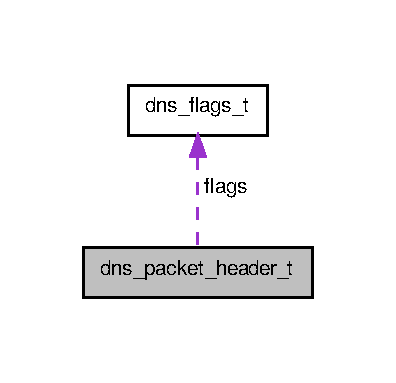
\includegraphics[width=190pt]{structdns__packet__header__t__coll__graph}
\end{center}
\end{figure}
\subsection*{Data Fields}
\begin{DoxyCompactItemize}
\item 
uint16\-\_\-t \hyperlink{structdns__packet__header__t_a4fc3a0c58dfbd1e68224521185cb9384}{id}
\item 
\hyperlink{structdns__flags__t}{dns\-\_\-flags\-\_\-t} \hyperlink{structdns__packet__header__t_a17537773eff778e034c52ba8bc8c2691}{flags}
\item 
uint16\-\_\-t \hyperlink{structdns__packet__header__t_a04016da27d1b8b5859d8527d2742f4f4}{qdcount}
\item 
uint16\-\_\-t \hyperlink{structdns__packet__header__t_a2a5577b198ba758438292038bbab5437}{ancount}
\item 
uint16\-\_\-t \hyperlink{structdns__packet__header__t_aa613b2dc181144b8d4c975a5260d59e3}{nscount}
\item 
uint16\-\_\-t \hyperlink{structdns__packet__header__t_a6eedffaf6f8d915f67e6f6bb77094562}{arcount}
\end{DoxyCompactItemize}


\subsection{Detailed Description}
D\-N\-S Packet header. 

The header of a D\-N\-S packet. 

Definition at line 69 of file mdns.\-h.



\subsection{Field Documentation}
\hypertarget{structdns__packet__header__t_a2a5577b198ba758438292038bbab5437}{\index{dns\-\_\-packet\-\_\-header\-\_\-t@{dns\-\_\-packet\-\_\-header\-\_\-t}!ancount@{ancount}}
\index{ancount@{ancount}!dns_packet_header_t@{dns\-\_\-packet\-\_\-header\-\_\-t}}
\subsubsection[{ancount}]{\setlength{\rightskip}{0pt plus 5cm}uint16\-\_\-t ancount}}\label{structdns__packet__header__t_a2a5577b198ba758438292038bbab5437}


Definition at line 73 of file mdns.\-h.

\hypertarget{structdns__packet__header__t_a6eedffaf6f8d915f67e6f6bb77094562}{\index{dns\-\_\-packet\-\_\-header\-\_\-t@{dns\-\_\-packet\-\_\-header\-\_\-t}!arcount@{arcount}}
\index{arcount@{arcount}!dns_packet_header_t@{dns\-\_\-packet\-\_\-header\-\_\-t}}
\subsubsection[{arcount}]{\setlength{\rightskip}{0pt plus 5cm}uint16\-\_\-t arcount}}\label{structdns__packet__header__t_a6eedffaf6f8d915f67e6f6bb77094562}


Definition at line 75 of file mdns.\-h.

\hypertarget{structdns__packet__header__t_a17537773eff778e034c52ba8bc8c2691}{\index{dns\-\_\-packet\-\_\-header\-\_\-t@{dns\-\_\-packet\-\_\-header\-\_\-t}!flags@{flags}}
\index{flags@{flags}!dns_packet_header_t@{dns\-\_\-packet\-\_\-header\-\_\-t}}
\subsubsection[{flags}]{\setlength{\rightskip}{0pt plus 5cm}{\bf dns\-\_\-flags\-\_\-t} flags}}\label{structdns__packet__header__t_a17537773eff778e034c52ba8bc8c2691}


Definition at line 71 of file mdns.\-h.

\hypertarget{structdns__packet__header__t_a4fc3a0c58dfbd1e68224521185cb9384}{\index{dns\-\_\-packet\-\_\-header\-\_\-t@{dns\-\_\-packet\-\_\-header\-\_\-t}!id@{id}}
\index{id@{id}!dns_packet_header_t@{dns\-\_\-packet\-\_\-header\-\_\-t}}
\subsubsection[{id}]{\setlength{\rightskip}{0pt plus 5cm}uint16\-\_\-t id}}\label{structdns__packet__header__t_a4fc3a0c58dfbd1e68224521185cb9384}


Definition at line 70 of file mdns.\-h.

\hypertarget{structdns__packet__header__t_aa613b2dc181144b8d4c975a5260d59e3}{\index{dns\-\_\-packet\-\_\-header\-\_\-t@{dns\-\_\-packet\-\_\-header\-\_\-t}!nscount@{nscount}}
\index{nscount@{nscount}!dns_packet_header_t@{dns\-\_\-packet\-\_\-header\-\_\-t}}
\subsubsection[{nscount}]{\setlength{\rightskip}{0pt plus 5cm}uint16\-\_\-t nscount}}\label{structdns__packet__header__t_aa613b2dc181144b8d4c975a5260d59e3}


Definition at line 74 of file mdns.\-h.

\hypertarget{structdns__packet__header__t_a04016da27d1b8b5859d8527d2742f4f4}{\index{dns\-\_\-packet\-\_\-header\-\_\-t@{dns\-\_\-packet\-\_\-header\-\_\-t}!qdcount@{qdcount}}
\index{qdcount@{qdcount}!dns_packet_header_t@{dns\-\_\-packet\-\_\-header\-\_\-t}}
\subsubsection[{qdcount}]{\setlength{\rightskip}{0pt plus 5cm}uint16\-\_\-t qdcount}}\label{structdns__packet__header__t_a04016da27d1b8b5859d8527d2742f4f4}


Definition at line 72 of file mdns.\-h.



The documentation for this struct was generated from the following file\-:\begin{DoxyCompactItemize}
\item 
Ether\-X\-Tag/src/\hyperlink{mdns_8h}{mdns.\-h}\end{DoxyCompactItemize}

\hypertarget{structdns__packet__t}{\section{dns\-\_\-packet\-\_\-t Struct Reference}
\label{structdns__packet__t}\index{dns\-\_\-packet\-\_\-t@{dns\-\_\-packet\-\_\-t}}
}


D\-N\-S Packet.  




{\ttfamily \#include $<$mdns.\-h$>$}



Collaboration diagram for dns\-\_\-packet\-\_\-t\-:
\nopagebreak
\begin{figure}[H]
\begin{center}
\leavevmode
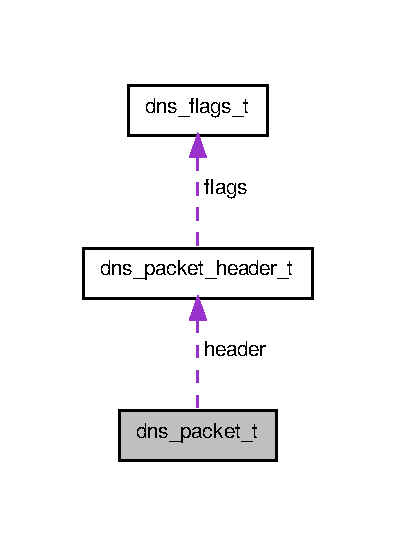
\includegraphics[width=190pt]{structdns__packet__t__coll__graph}
\end{center}
\end{figure}
\subsection*{Data Fields}
\begin{DoxyCompactItemize}
\item 
\hyperlink{structdns__packet__header__t}{dns\-\_\-packet\-\_\-header\-\_\-t} \hyperlink{structdns__packet__t_ae40246d3fea48323550a8957db1bd5c1}{header}
\item 
char $\ast$ \hyperlink{structdns__packet__t_a91a70b77df95bd8b0830b49a094c2acb}{data}
\item 
unsigned int $\ast$ \hyperlink{structdns__packet__t_a8053eea6cc5a03a184473df63560d978}{questions}
\item 
unsigned int $\ast$ \hyperlink{structdns__packet__t_ae0c9f53013dea2787cfdf2cff74b76ba}{answer\-\_\-rrs}
\item 
unsigned int $\ast$ \hyperlink{structdns__packet__t_abef983e2aec9c20ff1da712f4030fdba}{authority\-\_\-rrs}
\item 
unsigned int $\ast$ \hyperlink{structdns__packet__t_afa34bab568a73c5af6fc84ed676ed21f}{aditional\-\_\-rrs}
\end{DoxyCompactItemize}


\subsection{Detailed Description}
D\-N\-S Packet. 

D\-N\-S Packet header and payload 

Definition at line 82 of file mdns.\-h.



\subsection{Field Documentation}
\hypertarget{structdns__packet__t_afa34bab568a73c5af6fc84ed676ed21f}{\index{dns\-\_\-packet\-\_\-t@{dns\-\_\-packet\-\_\-t}!aditional\-\_\-rrs@{aditional\-\_\-rrs}}
\index{aditional\-\_\-rrs@{aditional\-\_\-rrs}!dns_packet_t@{dns\-\_\-packet\-\_\-t}}
\subsubsection[{aditional\-\_\-rrs}]{\setlength{\rightskip}{0pt plus 5cm}unsigned int$\ast$ aditional\-\_\-rrs}}\label{structdns__packet__t_afa34bab568a73c5af6fc84ed676ed21f}


Definition at line 88 of file mdns.\-h.

\hypertarget{structdns__packet__t_ae0c9f53013dea2787cfdf2cff74b76ba}{\index{dns\-\_\-packet\-\_\-t@{dns\-\_\-packet\-\_\-t}!answer\-\_\-rrs@{answer\-\_\-rrs}}
\index{answer\-\_\-rrs@{answer\-\_\-rrs}!dns_packet_t@{dns\-\_\-packet\-\_\-t}}
\subsubsection[{answer\-\_\-rrs}]{\setlength{\rightskip}{0pt plus 5cm}unsigned int$\ast$ answer\-\_\-rrs}}\label{structdns__packet__t_ae0c9f53013dea2787cfdf2cff74b76ba}


Definition at line 86 of file mdns.\-h.

\hypertarget{structdns__packet__t_abef983e2aec9c20ff1da712f4030fdba}{\index{dns\-\_\-packet\-\_\-t@{dns\-\_\-packet\-\_\-t}!authority\-\_\-rrs@{authority\-\_\-rrs}}
\index{authority\-\_\-rrs@{authority\-\_\-rrs}!dns_packet_t@{dns\-\_\-packet\-\_\-t}}
\subsubsection[{authority\-\_\-rrs}]{\setlength{\rightskip}{0pt plus 5cm}unsigned int$\ast$ authority\-\_\-rrs}}\label{structdns__packet__t_abef983e2aec9c20ff1da712f4030fdba}


Definition at line 87 of file mdns.\-h.

\hypertarget{structdns__packet__t_a91a70b77df95bd8b0830b49a094c2acb}{\index{dns\-\_\-packet\-\_\-t@{dns\-\_\-packet\-\_\-t}!data@{data}}
\index{data@{data}!dns_packet_t@{dns\-\_\-packet\-\_\-t}}
\subsubsection[{data}]{\setlength{\rightskip}{0pt plus 5cm}char$\ast$ data}}\label{structdns__packet__t_a91a70b77df95bd8b0830b49a094c2acb}


Definition at line 84 of file mdns.\-h.

\hypertarget{structdns__packet__t_ae40246d3fea48323550a8957db1bd5c1}{\index{dns\-\_\-packet\-\_\-t@{dns\-\_\-packet\-\_\-t}!header@{header}}
\index{header@{header}!dns_packet_t@{dns\-\_\-packet\-\_\-t}}
\subsubsection[{header}]{\setlength{\rightskip}{0pt plus 5cm}{\bf dns\-\_\-packet\-\_\-header\-\_\-t} header}}\label{structdns__packet__t_ae40246d3fea48323550a8957db1bd5c1}


Definition at line 83 of file mdns.\-h.

\hypertarget{structdns__packet__t_a8053eea6cc5a03a184473df63560d978}{\index{dns\-\_\-packet\-\_\-t@{dns\-\_\-packet\-\_\-t}!questions@{questions}}
\index{questions@{questions}!dns_packet_t@{dns\-\_\-packet\-\_\-t}}
\subsubsection[{questions}]{\setlength{\rightskip}{0pt plus 5cm}unsigned int$\ast$ questions}}\label{structdns__packet__t_a8053eea6cc5a03a184473df63560d978}


Definition at line 85 of file mdns.\-h.



The documentation for this struct was generated from the following file\-:\begin{DoxyCompactItemize}
\item 
Ether\-X\-Tag/src/\hyperlink{mdns_8h}{mdns.\-h}\end{DoxyCompactItemize}

\hypertarget{structjtag__response__t}{\section{jtag\-\_\-response\-\_\-t Struct Reference}
\label{structjtag__response__t}\index{jtag\-\_\-response\-\_\-t@{jtag\-\_\-response\-\_\-t}}
}


{\ttfamily \#include $<$dbg\-\_\-access.\-h$>$}

\subsection*{Data Fields}
\begin{DoxyCompactItemize}
\item 
unsigned int \hyperlink{structjtag__response__t_ac8d42bcd4a44e078047ccd7291059238}{length}
\item 
char $\ast$ \hyperlink{structjtag__response__t_a9e58a401fae91865c68ca3136c23808a}{data} \mbox{[}\hyperlink{dbg__cmd_8h_abe6cfb003699e267c6bb15e549e269a4}{M\-A\-X\-\_\-\-D\-B\-G\-\_\-\-C\-M\-D\-\_\-\-L\-E\-N}\mbox{]}
\end{DoxyCompactItemize}


\subsection{Detailed Description}


Definition at line 5 of file dbg\-\_\-access.\-h.



\subsection{Field Documentation}
\hypertarget{structjtag__response__t_a9e58a401fae91865c68ca3136c23808a}{\index{jtag\-\_\-response\-\_\-t@{jtag\-\_\-response\-\_\-t}!data@{data}}
\index{data@{data}!jtag_response_t@{jtag\-\_\-response\-\_\-t}}
\subsubsection[{data}]{\setlength{\rightskip}{0pt plus 5cm}char$\ast$ data\mbox{[}{\bf M\-A\-X\-\_\-\-D\-B\-G\-\_\-\-C\-M\-D\-\_\-\-L\-E\-N}\mbox{]}}}\label{structjtag__response__t_a9e58a401fae91865c68ca3136c23808a}


Definition at line 7 of file dbg\-\_\-access.\-h.

\hypertarget{structjtag__response__t_ac8d42bcd4a44e078047ccd7291059238}{\index{jtag\-\_\-response\-\_\-t@{jtag\-\_\-response\-\_\-t}!length@{length}}
\index{length@{length}!jtag_response_t@{jtag\-\_\-response\-\_\-t}}
\subsubsection[{length}]{\setlength{\rightskip}{0pt plus 5cm}unsigned int length}}\label{structjtag__response__t_ac8d42bcd4a44e078047ccd7291059238}


Definition at line 6 of file dbg\-\_\-access.\-h.



The documentation for this struct was generated from the following file\-:\begin{DoxyCompactItemize}
\item 
Ether\-X\-Tag/src/\hyperlink{dbg__access_8h}{dbg\-\_\-access.\-h}\end{DoxyCompactItemize}

\hypertarget{structpage__t}{\section{page\-\_\-t Struct Reference}
\label{structpage__t}\index{page\-\_\-t@{page\-\_\-t}}
}


{\ttfamily \#include $<$web\-\_\-service.\-h$>$}

\subsection*{Data Fields}
\begin{DoxyCompactItemize}
\item 
unsigned int \hyperlink{structpage__t_ac8d42bcd4a44e078047ccd7291059238}{length}
\item 
char $\ast$ \hyperlink{structpage__t_a91a70b77df95bd8b0830b49a094c2acb}{data}
\end{DoxyCompactItemize}


\subsection{Detailed Description}


Definition at line 4 of file web\-\_\-service.\-h.



\subsection{Field Documentation}
\hypertarget{structpage__t_a91a70b77df95bd8b0830b49a094c2acb}{\index{page\-\_\-t@{page\-\_\-t}!data@{data}}
\index{data@{data}!page_t@{page\-\_\-t}}
\subsubsection[{data}]{\setlength{\rightskip}{0pt plus 5cm}char$\ast$ data}}\label{structpage__t_a91a70b77df95bd8b0830b49a094c2acb}


Definition at line 6 of file web\-\_\-service.\-h.

\hypertarget{structpage__t_ac8d42bcd4a44e078047ccd7291059238}{\index{page\-\_\-t@{page\-\_\-t}!length@{length}}
\index{length@{length}!page_t@{page\-\_\-t}}
\subsubsection[{length}]{\setlength{\rightskip}{0pt plus 5cm}unsigned int length}}\label{structpage__t_ac8d42bcd4a44e078047ccd7291059238}


Definition at line 5 of file web\-\_\-service.\-h.



The documentation for this struct was generated from the following file\-:\begin{DoxyCompactItemize}
\item 
Ether\-X\-Tag/src/\hyperlink{web__service_8h}{web\-\_\-service.\-h}\end{DoxyCompactItemize}

\hypertarget{structsystem__state__t}{\section{system\-\_\-state\-\_\-t Struct Reference}
\label{structsystem__state__t}\index{system\-\_\-state\-\_\-t@{system\-\_\-state\-\_\-t}}
}


System state.  




{\ttfamily \#include $<$state.\-h$>$}

\subsection*{Data Fields}
\begin{DoxyCompactItemize}
\item 
char $\ast$ \hyperlink{structsystem__state__t_a5ccabdf4b4e4782c11b1a8262ddc2899}{current\-User}
\end{DoxyCompactItemize}


\subsection{Detailed Description}
System state. 

Represents the state of the system, including users, connected devices etc. 

Definition at line 8 of file state.\-h.



\subsection{Field Documentation}
\hypertarget{structsystem__state__t_a5ccabdf4b4e4782c11b1a8262ddc2899}{\index{system\-\_\-state\-\_\-t@{system\-\_\-state\-\_\-t}!current\-User@{current\-User}}
\index{current\-User@{current\-User}!system_state_t@{system\-\_\-state\-\_\-t}}
\subsubsection[{current\-User}]{\setlength{\rightskip}{0pt plus 5cm}char$\ast$ current\-User}}\label{structsystem__state__t_a5ccabdf4b4e4782c11b1a8262ddc2899}


Definition at line 9 of file state.\-h.



The documentation for this struct was generated from the following file\-:\begin{DoxyCompactItemize}
\item 
Ether\-X\-Tag/src/\hyperlink{state_8h}{state.\-h}\end{DoxyCompactItemize}

\chapter{File Documentation}
\hypertarget{dbg__access_8c}{\section{Ether\-X\-Tag/src/dbg\-\_\-access.c File Reference}
\label{dbg__access_8c}\index{Ether\-X\-Tag/src/dbg\-\_\-access.\-c@{Ether\-X\-Tag/src/dbg\-\_\-access.\-c}}
}
{\ttfamily \#include $<$string.\-h$>$}\\*
{\ttfamily \#include \char`\"{}dbg\-\_\-access.\-h\char`\"{}}\\*
Include dependency graph for dbg\-\_\-access.\-c\-:\nopagebreak
\begin{figure}[H]
\begin{center}
\leavevmode
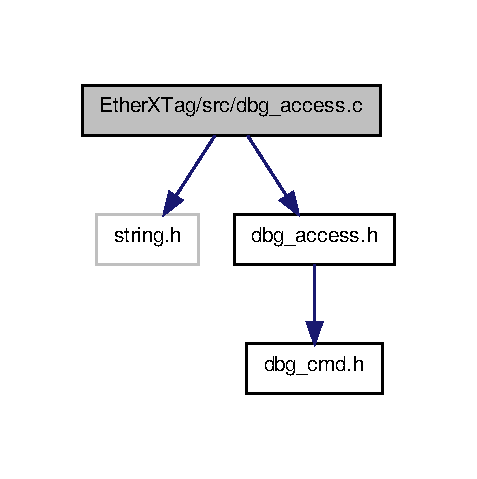
\includegraphics[width=229pt]{dbg__access_8c__incl}
\end{center}
\end{figure}
\subsection*{Functions}
\begin{DoxyCompactItemize}
\item 
\hyperlink{structjtag__response__t}{jtag\-\_\-response\-\_\-t} $\ast$ \hyperlink{dbg__access_8c_aba284c974550b4336a834170bf568d98}{get\-Response} (char $\ast$data, unsigned int len)
\end{DoxyCompactItemize}
\subsection*{Variables}
\begin{DoxyCompactItemize}
\item 
\hyperlink{structjtag__response__t}{jtag\-\_\-response\-\_\-t} \hyperlink{dbg__access_8c_a8f851130614b4e2713abea686d657f1e}{jt\-Ret\-Val} = \{ \}
\end{DoxyCompactItemize}


\subsection{Function Documentation}
\hypertarget{dbg__access_8c_aba284c974550b4336a834170bf568d98}{\index{dbg\-\_\-access.\-c@{dbg\-\_\-access.\-c}!get\-Response@{get\-Response}}
\index{get\-Response@{get\-Response}!dbg_access.c@{dbg\-\_\-access.\-c}}
\subsubsection[{get\-Response}]{\setlength{\rightskip}{0pt plus 5cm}{\bf jtag\-\_\-response\-\_\-t}$\ast$ get\-Response (
\begin{DoxyParamCaption}
\item[{char $\ast$}]{data, }
\item[{unsigned int}]{len}
\end{DoxyParamCaption}
)}}\label{dbg__access_8c_aba284c974550b4336a834170bf568d98}


Definition at line 8 of file dbg\-\_\-access.\-c.



\subsection{Variable Documentation}
\hypertarget{dbg__access_8c_a8f851130614b4e2713abea686d657f1e}{\index{dbg\-\_\-access.\-c@{dbg\-\_\-access.\-c}!jt\-Ret\-Val@{jt\-Ret\-Val}}
\index{jt\-Ret\-Val@{jt\-Ret\-Val}!dbg_access.c@{dbg\-\_\-access.\-c}}
\subsubsection[{jt\-Ret\-Val}]{\setlength{\rightskip}{0pt plus 5cm}{\bf jtag\-\_\-response\-\_\-t} jt\-Ret\-Val = \{ \}}}\label{dbg__access_8c_a8f851130614b4e2713abea686d657f1e}


Definition at line 6 of file dbg\-\_\-access.\-c.


\hypertarget{dbg__access_8h}{\section{Ether\-X\-Tag/src/dbg\-\_\-access.h File Reference}
\label{dbg__access_8h}\index{Ether\-X\-Tag/src/dbg\-\_\-access.\-h@{Ether\-X\-Tag/src/dbg\-\_\-access.\-h}}
}
{\ttfamily \#include \char`\"{}dbg\-\_\-cmd.\-h\char`\"{}}\\*
Include dependency graph for dbg\-\_\-access.\-h\-:\nopagebreak
\begin{figure}[H]
\begin{center}
\leavevmode
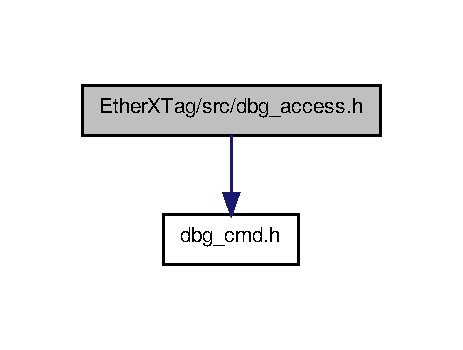
\includegraphics[width=222pt]{dbg__access_8h__incl}
\end{center}
\end{figure}
This graph shows which files directly or indirectly include this file\-:\nopagebreak
\begin{figure}[H]
\begin{center}
\leavevmode
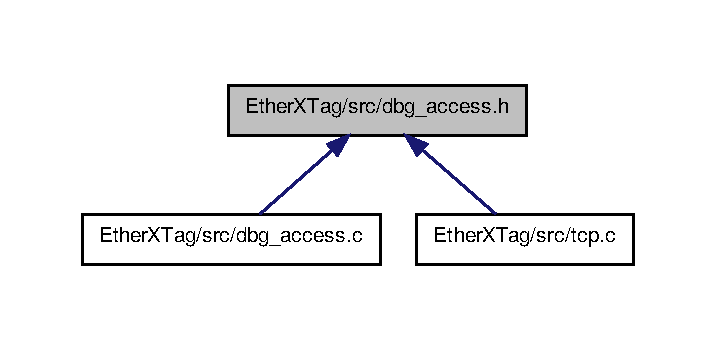
\includegraphics[width=344pt]{dbg__access_8h__dep__incl}
\end{center}
\end{figure}
\subsection*{Data Structures}
\begin{DoxyCompactItemize}
\item 
struct \hyperlink{structjtag__response__t}{jtag\-\_\-response\-\_\-t}
\end{DoxyCompactItemize}
\subsection*{Typedefs}
\begin{DoxyCompactItemize}
\item 
typedef struct \hyperlink{structjtag__response__t}{jtag\-\_\-response\-\_\-t} \hyperlink{dbg__access_8h_a547a882f60a3e3533482c99907535c79}{jtag\-\_\-response\-\_\-t}
\end{DoxyCompactItemize}
\subsection*{Functions}
\begin{DoxyCompactItemize}
\item 
\hyperlink{structjtag__response__t}{jtag\-\_\-response\-\_\-t} $\ast$ \hyperlink{dbg__access_8h_aba284c974550b4336a834170bf568d98}{get\-Response} (char $\ast$data, unsigned int len)
\end{DoxyCompactItemize}


\subsection{Typedef Documentation}
\hypertarget{dbg__access_8h_a547a882f60a3e3533482c99907535c79}{\index{dbg\-\_\-access.\-h@{dbg\-\_\-access.\-h}!jtag\-\_\-response\-\_\-t@{jtag\-\_\-response\-\_\-t}}
\index{jtag\-\_\-response\-\_\-t@{jtag\-\_\-response\-\_\-t}!dbg_access.h@{dbg\-\_\-access.\-h}}
\subsubsection[{jtag\-\_\-response\-\_\-t}]{\setlength{\rightskip}{0pt plus 5cm}typedef struct {\bf jtag\-\_\-response\-\_\-t}  {\bf jtag\-\_\-response\-\_\-t}}}\label{dbg__access_8h_a547a882f60a3e3533482c99907535c79}


\subsection{Function Documentation}
\hypertarget{dbg__access_8h_aba284c974550b4336a834170bf568d98}{\index{dbg\-\_\-access.\-h@{dbg\-\_\-access.\-h}!get\-Response@{get\-Response}}
\index{get\-Response@{get\-Response}!dbg_access.h@{dbg\-\_\-access.\-h}}
\subsubsection[{get\-Response}]{\setlength{\rightskip}{0pt plus 5cm}{\bf jtag\-\_\-response\-\_\-t}$\ast$ get\-Response (
\begin{DoxyParamCaption}
\item[{char $\ast$}]{data, }
\item[{unsigned int}]{len}
\end{DoxyParamCaption}
)}}\label{dbg__access_8h_aba284c974550b4336a834170bf568d98}


Definition at line 8 of file dbg\-\_\-access.\-c.


\hypertarget{dbg__cmd_8h}{\section{Ether\-X\-Tag/src/dbg\-\_\-cmd.h File Reference}
\label{dbg__cmd_8h}\index{Ether\-X\-Tag/src/dbg\-\_\-cmd.\-h@{Ether\-X\-Tag/src/dbg\-\_\-cmd.\-h}}
}
This graph shows which files directly or indirectly include this file\-:\nopagebreak
\begin{figure}[H]
\begin{center}
\leavevmode
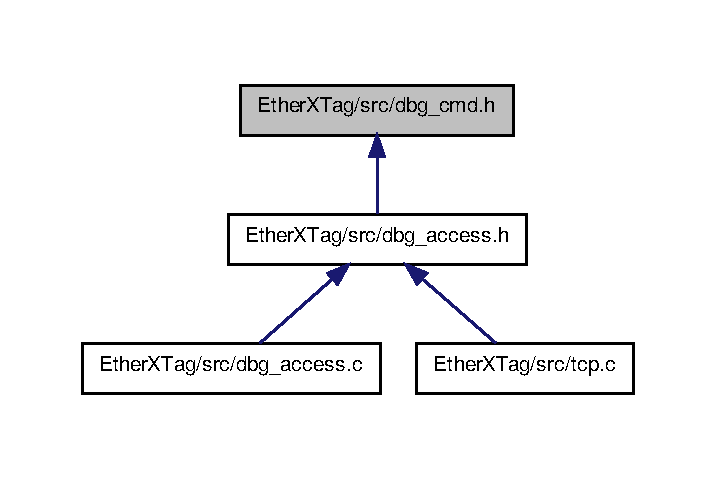
\includegraphics[width=344pt]{dbg__cmd_8h__dep__incl}
\end{center}
\end{figure}
\subsection*{Data Structures}
\begin{DoxyCompactItemize}
\item 
struct \hyperlink{structdbg__cmd__packet}{dbg\-\_\-cmd\-\_\-packet}
\item 
struct \hyperlink{structdbg__cmd__type__connect}{dbg\-\_\-cmd\-\_\-type\-\_\-connect}
\item 
struct \hyperlink{structdbg__cmd__type__disconnect}{dbg\-\_\-cmd\-\_\-type\-\_\-disconnect}
\item 
struct \hyperlink{structdbg__cmd__type__get__core__state}{dbg\-\_\-cmd\-\_\-type\-\_\-get\-\_\-core\-\_\-state}
\item 
struct \hyperlink{structdbg__cmd__type__enable__thread}{dbg\-\_\-cmd\-\_\-type\-\_\-enable\-\_\-thread}
\item 
struct \hyperlink{structdbg__cmd__type__disable__thread}{dbg\-\_\-cmd\-\_\-type\-\_\-disable\-\_\-thread}
\item 
struct \hyperlink{structdbg__cmd__type__read__regs}{dbg\-\_\-cmd\-\_\-type\-\_\-read\-\_\-regs}
\item 
struct \hyperlink{structdbg__cmd__type__write__regs}{dbg\-\_\-cmd\-\_\-type\-\_\-write\-\_\-regs}
\item 
struct \hyperlink{structdbg__cmd__type__read__mem}{dbg\-\_\-cmd\-\_\-type\-\_\-read\-\_\-mem}
\item 
struct \hyperlink{structdbg__cmd__type__write__mem}{dbg\-\_\-cmd\-\_\-type\-\_\-write\-\_\-mem}
\item 
struct \hyperlink{structdbg__cmd__type__read__obj}{dbg\-\_\-cmd\-\_\-type\-\_\-read\-\_\-obj}
\item 
struct \hyperlink{structdbg__cmd__type__step}{dbg\-\_\-cmd\-\_\-type\-\_\-step}
\item 
struct \hyperlink{structdbg__cmd__type__continue}{dbg\-\_\-cmd\-\_\-type\-\_\-continue}
\item 
struct \hyperlink{structdbg__cmd__type__add__break}{dbg\-\_\-cmd\-\_\-type\-\_\-add\-\_\-break}
\item 
struct \hyperlink{structdbg__cmd__type__remove__break}{dbg\-\_\-cmd\-\_\-type\-\_\-remove\-\_\-break}
\item 
struct \hyperlink{structdbg__cmd__type__get__status}{dbg\-\_\-cmd\-\_\-type\-\_\-get\-\_\-status}
\item 
struct \hyperlink{structdbg__cmd__type__interrupt}{dbg\-\_\-cmd\-\_\-type\-\_\-interrupt}
\item 
struct \hyperlink{structdbg__cmd__type__reset}{dbg\-\_\-cmd\-\_\-type\-\_\-reset}
\item 
struct \hyperlink{structdbg__cmd__type__firmware__version}{dbg\-\_\-cmd\-\_\-type\-\_\-firmware\-\_\-version}
\item 
struct \hyperlink{structdbg__cmd__type__firmware__reboot}{dbg\-\_\-cmd\-\_\-type\-\_\-firmware\-\_\-reboot}
\item 
struct \hyperlink{structdbg__cmd__type__read__jtag__reg}{dbg\-\_\-cmd\-\_\-type\-\_\-read\-\_\-jtag\-\_\-reg}
\item 
struct \hyperlink{structdbg__cmd__type__write__jtag__reg}{dbg\-\_\-cmd\-\_\-type\-\_\-write\-\_\-jtag\-\_\-reg}
\item 
struct \hyperlink{structdbg__cmd__type__get__jtag__chain}{dbg\-\_\-cmd\-\_\-type\-\_\-get\-\_\-jtag\-\_\-chain}
\item 
struct \hyperlink{structdbg__cmd__type__upload__xscope__data}{dbg\-\_\-cmd\-\_\-type\-\_\-upload\-\_\-xscope\-\_\-data}
\item 
struct \hyperlink{structdbg__cmd__type__connect__xscope__channel}{dbg\-\_\-cmd\-\_\-type\-\_\-connect\-\_\-xscope\-\_\-channel}
\item 
struct \hyperlink{structdbg__cmd__type__get__chip__info}{dbg\-\_\-cmd\-\_\-type\-\_\-get\-\_\-chip\-\_\-info}
\item 
struct \hyperlink{structdbg__cmd__type__jtag__pins}{dbg\-\_\-cmd\-\_\-type\-\_\-jtag\-\_\-pins}
\item 
struct \hyperlink{structdbg__cmd__type__jtag__pc__sample}{dbg\-\_\-cmd\-\_\-type\-\_\-jtag\-\_\-pc\-\_\-sample}
\end{DoxyCompactItemize}
\subsection*{Macros}
\begin{DoxyCompactItemize}
\item 
\#define \hyperlink{dbg__cmd_8h_abe6cfb003699e267c6bb15e549e269a4}{M\-A\-X\-\_\-\-D\-B\-G\-\_\-\-C\-M\-D\-\_\-\-L\-E\-N}~124
\item 
\#define \hyperlink{dbg__cmd_8h_a4552ec15033c8a68870cdf80eda5470c}{M\-A\-X\-\_\-\-D\-B\-G\-\_\-\-C\-M\-D\-\_\-\-D\-A\-T\-A\-\_\-\-L\-E\-N}~(\hyperlink{dbg__cmd_8h_abe6cfb003699e267c6bb15e549e269a4}{M\-A\-X\-\_\-\-D\-B\-G\-\_\-\-C\-M\-D\-\_\-\-L\-E\-N} -\/ 1)
\item 
\#define \hyperlink{dbg__cmd_8h_aab7ffac23cfbe44c03699c2e5d5fcd75}{D\-B\-G\-\_\-\-C\-M\-D\-\_\-\-F\-I\-R\-M\-W\-A\-R\-E\-\_\-\-V\-E\-R\-S\-I\-O\-N\-\_\-\-R\-E\-Q}~3
\item 
\#define \hyperlink{dbg__cmd_8h_a24ec609777392dba30a981cec663d025}{D\-B\-G\-\_\-\-C\-M\-D\-\_\-\-F\-I\-R\-M\-W\-A\-R\-E\-\_\-\-V\-E\-R\-S\-I\-O\-N\-\_\-\-A\-C\-K}~4
\item 
\#define \hyperlink{dbg__cmd_8h_ab7ab991376fede9d59ab9bcacd534801}{M\-A\-X\-\_\-\-D\-B\-G\-\_\-\-M\-E\-M\-\_\-\-T\-F\-R\-\_\-\-B\-L\-O\-C\-K}~(\hyperlink{dbg__cmd_8h_a4552ec15033c8a68870cdf80eda5470c}{M\-A\-X\-\_\-\-D\-B\-G\-\_\-\-C\-M\-D\-\_\-\-D\-A\-T\-A\-\_\-\-L\-E\-N}-\/3)
\item 
\#define \hyperlink{dbg__cmd_8h_af97c0773bc3eed0274f60931cfdd6239}{D\-B\-G\-\_\-\-M\-E\-M\-\_\-\-B\-R\-E\-A\-K}~0
\item 
\#define \hyperlink{dbg__cmd_8h_ac94f553d097f9a0ba356b3fe6e4403f4}{D\-B\-G\-\_\-\-W\-\_\-\-W\-A\-T\-C\-H\-\_\-\-B\-R\-E\-A\-K}~1
\item 
\#define \hyperlink{dbg__cmd_8h_aef1e60994f3bae29163647ed9e80159b}{D\-B\-G\-\_\-\-R\-\_\-\-W\-A\-T\-C\-H\-\_\-\-B\-R\-E\-A\-K}~2
\item 
\#define \hyperlink{dbg__cmd_8h_a44eaa96ad717195df177413e3a86e2d6}{D\-B\-G\-\_\-\-A\-\_\-\-W\-A\-T\-C\-H\-\_\-\-B\-R\-E\-A\-K}~3
\item 
\#define \hyperlink{dbg__cmd_8h_a4fcf61bae68d93b22dc29178c39fe841}{D\-B\-G\-\_\-\-R\-E\-S\-\_\-\-W\-A\-T\-C\-H\-\_\-\-B\-R\-E\-A\-K}~4
\end{DoxyCompactItemize}
\subsection*{Enumerations}
\begin{DoxyCompactItemize}
\item 
enum \hyperlink{dbg__cmd_8h_a921a01d6be6d3bf1d52a1713a55b186d}{dbg\-\_\-cmd\-\_\-type} \{ \\*
\hyperlink{dbg__cmd_8h_a921a01d6be6d3bf1d52a1713a55b186dad8abbd2710cb8e343d776fccf31a02ad}{D\-B\-G\-\_\-\-C\-M\-D\-\_\-\-N\-O\-N\-E}, 
\hyperlink{dbg__cmd_8h_a921a01d6be6d3bf1d52a1713a55b186daf55f7d28badf26713bca5ece64e2a380}{D\-B\-G\-\_\-\-C\-M\-D\-\_\-\-C\-O\-N\-N\-E\-C\-T\-\_\-\-R\-E\-Q}, 
\hyperlink{dbg__cmd_8h_a921a01d6be6d3bf1d52a1713a55b186da9d83fd095d10570c67f4f529e375d7c3}{D\-B\-G\-\_\-\-C\-M\-D\-\_\-\-C\-O\-N\-N\-E\-C\-T\-\_\-\-A\-C\-K}, 
\hyperlink{dbg__cmd_8h_a921a01d6be6d3bf1d52a1713a55b186dae8e0701a0d919bee71e5859dcad9c954}{D\-B\-G\-\_\-\-C\-M\-D\-\_\-\-D\-I\-S\-C\-O\-N\-N\-E\-C\-T\-\_\-\-R\-E\-Q}, 
\\*
\hyperlink{dbg__cmd_8h_a921a01d6be6d3bf1d52a1713a55b186da971e2231a07bf20015dc73c06e5f6750}{D\-B\-G\-\_\-\-C\-M\-D\-\_\-\-D\-I\-S\-C\-O\-N\-N\-E\-C\-T\-\_\-\-A\-C\-K}, 
\hyperlink{dbg__cmd_8h_a921a01d6be6d3bf1d52a1713a55b186da1cc17c4c09936672ac7d2ebacff3df1e}{D\-B\-G\-\_\-\-C\-M\-D\-\_\-\-G\-E\-T\-\_\-\-C\-O\-R\-E\-\_\-\-S\-T\-A\-T\-E\-\_\-\-R\-E\-Q}, 
\hyperlink{dbg__cmd_8h_a921a01d6be6d3bf1d52a1713a55b186da5611009aaaf539f4ff1479144c4a6526}{D\-B\-G\-\_\-\-C\-M\-D\-\_\-\-G\-E\-T\-\_\-\-C\-O\-R\-E\-\_\-\-S\-T\-A\-T\-E\-\_\-\-A\-C\-K}, 
\hyperlink{dbg__cmd_8h_a921a01d6be6d3bf1d52a1713a55b186daf6a95aa241b4db85c0b38f854818a6df}{D\-B\-G\-\_\-\-C\-M\-D\-\_\-\-E\-N\-A\-B\-L\-E\-\_\-\-T\-H\-R\-E\-A\-D\-\_\-\-R\-E\-Q}, 
\\*
\hyperlink{dbg__cmd_8h_a921a01d6be6d3bf1d52a1713a55b186daf6f104a4669cb2494d489484000c4b85}{D\-B\-G\-\_\-\-C\-M\-D\-\_\-\-E\-N\-A\-B\-L\-E\-\_\-\-T\-H\-R\-E\-A\-D\-\_\-\-A\-C\-K}, 
\hyperlink{dbg__cmd_8h_a921a01d6be6d3bf1d52a1713a55b186da11b313c952f4c7e0ed54586877c8ffe0}{D\-B\-G\-\_\-\-C\-M\-D\-\_\-\-D\-I\-S\-A\-B\-L\-E\-\_\-\-T\-H\-R\-E\-A\-D\-\_\-\-R\-E\-Q}, 
\hyperlink{dbg__cmd_8h_a921a01d6be6d3bf1d52a1713a55b186da0143b7aeaee45dcc055c6f0f592434d5}{D\-B\-G\-\_\-\-C\-M\-D\-\_\-\-D\-I\-S\-A\-B\-L\-E\-\_\-\-T\-H\-R\-E\-A\-D\-\_\-\-A\-C\-K}, 
\hyperlink{dbg__cmd_8h_a921a01d6be6d3bf1d52a1713a55b186da290bd53612c49ccdac1b5ba6b3344f35}{D\-B\-G\-\_\-\-C\-M\-D\-\_\-\-R\-E\-A\-D\-\_\-\-R\-E\-G\-S\-\_\-\-R\-E\-Q}, 
\\*
\hyperlink{dbg__cmd_8h_a921a01d6be6d3bf1d52a1713a55b186da593596d30ad5cb0dd69f06a3d77255f7}{D\-B\-G\-\_\-\-C\-M\-D\-\_\-\-R\-E\-A\-D\-\_\-\-R\-E\-G\-S\-\_\-\-A\-C\-K}, 
\hyperlink{dbg__cmd_8h_a921a01d6be6d3bf1d52a1713a55b186daf173a0201b0b98813e29b36897dc48f7}{D\-B\-G\-\_\-\-C\-M\-D\-\_\-\-W\-R\-I\-T\-E\-\_\-\-R\-E\-G\-S\-\_\-\-R\-E\-Q}, 
\hyperlink{dbg__cmd_8h_a921a01d6be6d3bf1d52a1713a55b186da6ac4f74b2f34f2009328e12464c2ef01}{D\-B\-G\-\_\-\-C\-M\-D\-\_\-\-W\-R\-I\-T\-E\-\_\-\-R\-E\-G\-S\-\_\-\-A\-C\-K}, 
\hyperlink{dbg__cmd_8h_a921a01d6be6d3bf1d52a1713a55b186da4d84002843e0459c2e92f495a069dae1}{D\-B\-G\-\_\-\-C\-M\-D\-\_\-\-R\-E\-A\-D\-\_\-\-M\-E\-M\-\_\-\-R\-E\-Q} =  100, 
\\*
\hyperlink{dbg__cmd_8h_a921a01d6be6d3bf1d52a1713a55b186da46a38ba8868c2f847e1650c131d7e28d}{D\-B\-G\-\_\-\-C\-M\-D\-\_\-\-R\-E\-A\-D\-\_\-\-M\-E\-M\-\_\-\-A\-C\-K}, 
\hyperlink{dbg__cmd_8h_a921a01d6be6d3bf1d52a1713a55b186da9622bf8e4136ba2ceb1ebbe846816415}{D\-B\-G\-\_\-\-C\-M\-D\-\_\-\-W\-R\-I\-T\-E\-\_\-\-M\-E\-M\-\_\-\-R\-E\-Q}, 
\hyperlink{dbg__cmd_8h_a921a01d6be6d3bf1d52a1713a55b186dabd7e7ae1e8dbda266605c999b818a91b}{D\-B\-G\-\_\-\-C\-M\-D\-\_\-\-W\-R\-I\-T\-E\-\_\-\-M\-E\-M\-\_\-\-A\-C\-K}, 
\hyperlink{dbg__cmd_8h_a921a01d6be6d3bf1d52a1713a55b186dad94798306a8273c790de9bdc43e6bf27}{D\-B\-G\-\_\-\-C\-M\-D\-\_\-\-R\-E\-A\-D\-\_\-\-O\-B\-J\-\_\-\-R\-E\-Q}, 
\\*
\hyperlink{dbg__cmd_8h_a921a01d6be6d3bf1d52a1713a55b186daaab58710389ee2e02ee8a3b04f0a19c5}{D\-B\-G\-\_\-\-C\-M\-D\-\_\-\-R\-E\-A\-D\-\_\-\-O\-B\-J\-\_\-\-A\-C\-K}, 
\hyperlink{dbg__cmd_8h_a921a01d6be6d3bf1d52a1713a55b186dad887ff38fc215f32b630149edf613c7a}{D\-B\-G\-\_\-\-C\-M\-D\-\_\-\-S\-T\-E\-P\-\_\-\-R\-E\-Q}, 
\hyperlink{dbg__cmd_8h_a921a01d6be6d3bf1d52a1713a55b186da331a3da230ae0a01865699c9b71d4d07}{D\-B\-G\-\_\-\-C\-M\-D\-\_\-\-S\-T\-E\-P\-\_\-\-A\-C\-K}, 
\hyperlink{dbg__cmd_8h_a921a01d6be6d3bf1d52a1713a55b186da26accf1f59cb2e3f48d8442ed0161d74}{D\-B\-G\-\_\-\-C\-M\-D\-\_\-\-C\-O\-N\-T\-I\-N\-U\-E\-\_\-\-R\-E\-Q}, 
\\*
\hyperlink{dbg__cmd_8h_a921a01d6be6d3bf1d52a1713a55b186da2f55d2176fb1bc7bf8577d70363f89e8}{D\-B\-G\-\_\-\-C\-M\-D\-\_\-\-C\-O\-N\-T\-I\-N\-U\-E\-\_\-\-A\-C\-K}, 
\hyperlink{dbg__cmd_8h_a921a01d6be6d3bf1d52a1713a55b186da765c264f4ca7acf865bca4e4a706c957}{D\-B\-G\-\_\-\-C\-M\-D\-\_\-\-A\-D\-D\-\_\-\-B\-R\-E\-A\-K\-\_\-\-R\-E\-Q}, 
\hyperlink{dbg__cmd_8h_a921a01d6be6d3bf1d52a1713a55b186da455ea5c75f7fd75e337b1f929700007a}{D\-B\-G\-\_\-\-C\-M\-D\-\_\-\-A\-D\-D\-\_\-\-B\-R\-E\-A\-K\-\_\-\-A\-C\-K}, 
\hyperlink{dbg__cmd_8h_a921a01d6be6d3bf1d52a1713a55b186da1414e3e64a723b3425b3d6010f18ebf6}{D\-B\-G\-\_\-\-C\-M\-D\-\_\-\-R\-E\-M\-O\-V\-E\-\_\-\-B\-R\-E\-A\-K\-\_\-\-R\-E\-Q}, 
\\*
\hyperlink{dbg__cmd_8h_a921a01d6be6d3bf1d52a1713a55b186da41f58e019897015aefbbe46e48932a83}{D\-B\-G\-\_\-\-C\-M\-D\-\_\-\-R\-E\-M\-O\-V\-E\-\_\-\-B\-R\-E\-A\-K\-\_\-\-A\-C\-K}, 
\hyperlink{dbg__cmd_8h_a921a01d6be6d3bf1d52a1713a55b186da976419a9efc112c7b57c5c64b2c86677}{D\-B\-G\-\_\-\-C\-M\-D\-\_\-\-G\-E\-T\-\_\-\-S\-T\-A\-T\-U\-S\-\_\-\-R\-E\-Q}, 
\hyperlink{dbg__cmd_8h_a921a01d6be6d3bf1d52a1713a55b186da6d9149917ad2f14c329585d3b6287a60}{D\-B\-G\-\_\-\-C\-M\-D\-\_\-\-G\-E\-T\-\_\-\-S\-T\-A\-T\-U\-S\-\_\-\-A\-C\-K}, 
\hyperlink{dbg__cmd_8h_a921a01d6be6d3bf1d52a1713a55b186daf0c2fc454ae8b91f5a4313d7c4a9a37f}{D\-B\-G\-\_\-\-C\-M\-D\-\_\-\-I\-N\-T\-E\-R\-R\-U\-P\-T\-\_\-\-R\-E\-Q}, 
\\*
\hyperlink{dbg__cmd_8h_a921a01d6be6d3bf1d52a1713a55b186da648520227f628010453f788194519032}{D\-B\-G\-\_\-\-C\-M\-D\-\_\-\-I\-N\-T\-E\-R\-R\-U\-P\-T\-\_\-\-A\-C\-K}, 
\hyperlink{dbg__cmd_8h_a921a01d6be6d3bf1d52a1713a55b186dad18a356cc516c329e936c982a17f1170}{D\-B\-G\-\_\-\-C\-M\-D\-\_\-\-R\-E\-S\-E\-T\-\_\-\-R\-E\-Q}, 
\hyperlink{dbg__cmd_8h_a921a01d6be6d3bf1d52a1713a55b186da41ec6f73f052808cee494287791d9d9e}{D\-B\-G\-\_\-\-C\-M\-D\-\_\-\-R\-E\-S\-E\-T\-\_\-\-A\-C\-K}, 
\hyperlink{dbg__cmd_8h_a921a01d6be6d3bf1d52a1713a55b186dacb3a11b328a4db6ff503704a68fee80a}{D\-B\-G\-\_\-\-C\-M\-D\-\_\-\-R\-E\-A\-D\-\_\-\-J\-T\-A\-G\-\_\-\-R\-E\-G\-\_\-\-R\-E\-Q}, 
\\*
\hyperlink{dbg__cmd_8h_a921a01d6be6d3bf1d52a1713a55b186da78713b4fe9a7cfaaa42444c716a37de8}{D\-B\-G\-\_\-\-C\-M\-D\-\_\-\-R\-E\-A\-D\-\_\-\-J\-T\-A\-G\-\_\-\-R\-E\-G\-\_\-\-A\-C\-K}, 
\hyperlink{dbg__cmd_8h_a921a01d6be6d3bf1d52a1713a55b186da7e07007acdf6b350a949c060721a83c6}{D\-B\-G\-\_\-\-C\-M\-D\-\_\-\-W\-R\-I\-T\-E\-\_\-\-J\-T\-A\-G\-\_\-\-R\-E\-G\-\_\-\-R\-E\-Q}, 
\hyperlink{dbg__cmd_8h_a921a01d6be6d3bf1d52a1713a55b186da29ee27f6393fdd13b910380fa9580d67}{D\-B\-G\-\_\-\-C\-M\-D\-\_\-\-W\-R\-I\-T\-E\-\_\-\-J\-T\-A\-G\-\_\-\-R\-E\-G\-\_\-\-A\-C\-K}, 
\hyperlink{dbg__cmd_8h_a921a01d6be6d3bf1d52a1713a55b186da3a0268faaefa18cef42089b0e43532d3}{D\-B\-G\-\_\-\-C\-M\-D\-\_\-\-G\-E\-T\-\_\-\-J\-T\-A\-G\-\_\-\-C\-H\-A\-I\-N\-\_\-\-R\-E\-Q}, 
\\*
\hyperlink{dbg__cmd_8h_a921a01d6be6d3bf1d52a1713a55b186da57dd138efac195e06d50d7a1a99c3f0f}{D\-B\-G\-\_\-\-C\-M\-D\-\_\-\-G\-E\-T\-\_\-\-J\-T\-A\-G\-\_\-\-C\-H\-A\-I\-N\-\_\-\-A\-C\-K}, 
\hyperlink{dbg__cmd_8h_a921a01d6be6d3bf1d52a1713a55b186daa0b46d29adb639d06e4280f240f5103b}{D\-B\-G\-\_\-\-C\-M\-D\-\_\-\-G\-E\-T\-\_\-\-C\-H\-I\-P\-\_\-\-I\-N\-F\-O\-\_\-\-R\-E\-Q}, 
\hyperlink{dbg__cmd_8h_a921a01d6be6d3bf1d52a1713a55b186da7f9f73e7d2b67f779d4a7504aa1bfdc9}{D\-B\-G\-\_\-\-C\-M\-D\-\_\-\-G\-E\-T\-\_\-\-C\-H\-I\-P\-\_\-\-I\-N\-F\-O\-\_\-\-A\-C\-K}, 
\hyperlink{dbg__cmd_8h_a921a01d6be6d3bf1d52a1713a55b186da39451e941c1314fea11cd34267bb5cc2}{D\-B\-G\-\_\-\-C\-M\-D\-\_\-\-J\-T\-A\-G\-\_\-\-P\-I\-N\-S\-\_\-\-R\-E\-Q}, 
\\*
\hyperlink{dbg__cmd_8h_a921a01d6be6d3bf1d52a1713a55b186dac847d125397cce331a4a0bd3991af0f4}{D\-B\-G\-\_\-\-C\-M\-D\-\_\-\-J\-T\-A\-G\-\_\-\-P\-I\-N\-S\-\_\-\-A\-C\-K}, 
\hyperlink{dbg__cmd_8h_a921a01d6be6d3bf1d52a1713a55b186dac11d22aa03c9f81627bbfb646e25df0b}{D\-B\-G\-\_\-\-C\-M\-D\-\_\-\-J\-T\-A\-G\-\_\-\-P\-C\-\_\-\-S\-A\-M\-P\-L\-E\-\_\-\-R\-E\-Q}, 
\hyperlink{dbg__cmd_8h_a921a01d6be6d3bf1d52a1713a55b186da69a761a2ffbe8df34bd39ff9272e7d66}{D\-B\-G\-\_\-\-C\-M\-D\-\_\-\-J\-T\-A\-G\-\_\-\-P\-C\-\_\-\-S\-A\-M\-P\-L\-E\-\_\-\-A\-C\-K}, 
\hyperlink{dbg__cmd_8h_a921a01d6be6d3bf1d52a1713a55b186da0dc6b0db874728aa2fb838685c723d70}{D\-B\-G\-\_\-\-C\-M\-D\-\_\-\-U\-P\-L\-O\-A\-D\-\_\-\-X\-S\-C\-O\-P\-E\-\_\-\-D\-A\-T\-A\-\_\-\-R\-E\-Q}, 
\\*
\hyperlink{dbg__cmd_8h_a921a01d6be6d3bf1d52a1713a55b186da41871ca789656893514fd78f7c2b2e30}{D\-B\-G\-\_\-\-C\-M\-D\-\_\-\-U\-P\-L\-O\-A\-D\-\_\-\-X\-S\-C\-O\-P\-E\-\_\-\-D\-A\-T\-A\-\_\-\-A\-C\-K}, 
\hyperlink{dbg__cmd_8h_a921a01d6be6d3bf1d52a1713a55b186da7547d938c035ea994bf5ea82b4e6c645}{D\-B\-G\-\_\-\-C\-M\-D\-\_\-\-C\-O\-N\-N\-E\-C\-T\-\_\-\-X\-S\-C\-O\-P\-E\-\_\-\-C\-H\-A\-N\-N\-E\-L\-\_\-\-R\-E\-Q}, 
\hyperlink{dbg__cmd_8h_a921a01d6be6d3bf1d52a1713a55b186da82781048591c0a0e862f8359a1b72703}{D\-B\-G\-\_\-\-C\-M\-D\-\_\-\-C\-O\-N\-N\-E\-C\-T\-\_\-\-X\-S\-C\-O\-P\-E\-\_\-\-C\-H\-A\-N\-N\-E\-L\-\_\-\-A\-C\-K}, 
\hyperlink{dbg__cmd_8h_a921a01d6be6d3bf1d52a1713a55b186dadd13f0f1838e1780161cd73bc7f4991f}{D\-B\-G\-\_\-\-C\-M\-D\-\_\-\-F\-I\-R\-M\-W\-A\-R\-E\-\_\-\-R\-E\-B\-O\-O\-T\-\_\-\-R\-E\-Q}, 
\\*
\hyperlink{dbg__cmd_8h_a921a01d6be6d3bf1d52a1713a55b186daee29e46346c2b7077a7504b9a7a2034c}{D\-B\-G\-\_\-\-C\-M\-D\-\_\-\-F\-I\-R\-M\-W\-A\-R\-E\-\_\-\-R\-E\-B\-O\-O\-T\-\_\-\-A\-C\-K}
 \}
\end{DoxyCompactItemize}


\subsection{Macro Definition Documentation}
\hypertarget{dbg__cmd_8h_a44eaa96ad717195df177413e3a86e2d6}{\index{dbg\-\_\-cmd.\-h@{dbg\-\_\-cmd.\-h}!D\-B\-G\-\_\-\-A\-\_\-\-W\-A\-T\-C\-H\-\_\-\-B\-R\-E\-A\-K@{D\-B\-G\-\_\-\-A\-\_\-\-W\-A\-T\-C\-H\-\_\-\-B\-R\-E\-A\-K}}
\index{D\-B\-G\-\_\-\-A\-\_\-\-W\-A\-T\-C\-H\-\_\-\-B\-R\-E\-A\-K@{D\-B\-G\-\_\-\-A\-\_\-\-W\-A\-T\-C\-H\-\_\-\-B\-R\-E\-A\-K}!dbg_cmd.h@{dbg\-\_\-cmd.\-h}}
\subsubsection[{D\-B\-G\-\_\-\-A\-\_\-\-W\-A\-T\-C\-H\-\_\-\-B\-R\-E\-A\-K}]{\setlength{\rightskip}{0pt plus 5cm}\#define D\-B\-G\-\_\-\-A\-\_\-\-W\-A\-T\-C\-H\-\_\-\-B\-R\-E\-A\-K~3}}\label{dbg__cmd_8h_a44eaa96ad717195df177413e3a86e2d6}


Definition at line 162 of file dbg\-\_\-cmd.\-h.

\hypertarget{dbg__cmd_8h_a24ec609777392dba30a981cec663d025}{\index{dbg\-\_\-cmd.\-h@{dbg\-\_\-cmd.\-h}!D\-B\-G\-\_\-\-C\-M\-D\-\_\-\-F\-I\-R\-M\-W\-A\-R\-E\-\_\-\-V\-E\-R\-S\-I\-O\-N\-\_\-\-A\-C\-K@{D\-B\-G\-\_\-\-C\-M\-D\-\_\-\-F\-I\-R\-M\-W\-A\-R\-E\-\_\-\-V\-E\-R\-S\-I\-O\-N\-\_\-\-A\-C\-K}}
\index{D\-B\-G\-\_\-\-C\-M\-D\-\_\-\-F\-I\-R\-M\-W\-A\-R\-E\-\_\-\-V\-E\-R\-S\-I\-O\-N\-\_\-\-A\-C\-K@{D\-B\-G\-\_\-\-C\-M\-D\-\_\-\-F\-I\-R\-M\-W\-A\-R\-E\-\_\-\-V\-E\-R\-S\-I\-O\-N\-\_\-\-A\-C\-K}!dbg_cmd.h@{dbg\-\_\-cmd.\-h}}
\subsubsection[{D\-B\-G\-\_\-\-C\-M\-D\-\_\-\-F\-I\-R\-M\-W\-A\-R\-E\-\_\-\-V\-E\-R\-S\-I\-O\-N\-\_\-\-A\-C\-K}]{\setlength{\rightskip}{0pt plus 5cm}\#define D\-B\-G\-\_\-\-C\-M\-D\-\_\-\-F\-I\-R\-M\-W\-A\-R\-E\-\_\-\-V\-E\-R\-S\-I\-O\-N\-\_\-\-A\-C\-K~4}}\label{dbg__cmd_8h_a24ec609777392dba30a981cec663d025}


Definition at line 14 of file dbg\-\_\-cmd.\-h.

\hypertarget{dbg__cmd_8h_aab7ffac23cfbe44c03699c2e5d5fcd75}{\index{dbg\-\_\-cmd.\-h@{dbg\-\_\-cmd.\-h}!D\-B\-G\-\_\-\-C\-M\-D\-\_\-\-F\-I\-R\-M\-W\-A\-R\-E\-\_\-\-V\-E\-R\-S\-I\-O\-N\-\_\-\-R\-E\-Q@{D\-B\-G\-\_\-\-C\-M\-D\-\_\-\-F\-I\-R\-M\-W\-A\-R\-E\-\_\-\-V\-E\-R\-S\-I\-O\-N\-\_\-\-R\-E\-Q}}
\index{D\-B\-G\-\_\-\-C\-M\-D\-\_\-\-F\-I\-R\-M\-W\-A\-R\-E\-\_\-\-V\-E\-R\-S\-I\-O\-N\-\_\-\-R\-E\-Q@{D\-B\-G\-\_\-\-C\-M\-D\-\_\-\-F\-I\-R\-M\-W\-A\-R\-E\-\_\-\-V\-E\-R\-S\-I\-O\-N\-\_\-\-R\-E\-Q}!dbg_cmd.h@{dbg\-\_\-cmd.\-h}}
\subsubsection[{D\-B\-G\-\_\-\-C\-M\-D\-\_\-\-F\-I\-R\-M\-W\-A\-R\-E\-\_\-\-V\-E\-R\-S\-I\-O\-N\-\_\-\-R\-E\-Q}]{\setlength{\rightskip}{0pt plus 5cm}\#define D\-B\-G\-\_\-\-C\-M\-D\-\_\-\-F\-I\-R\-M\-W\-A\-R\-E\-\_\-\-V\-E\-R\-S\-I\-O\-N\-\_\-\-R\-E\-Q~3}}\label{dbg__cmd_8h_aab7ffac23cfbe44c03699c2e5d5fcd75}


Definition at line 13 of file dbg\-\_\-cmd.\-h.

\hypertarget{dbg__cmd_8h_af97c0773bc3eed0274f60931cfdd6239}{\index{dbg\-\_\-cmd.\-h@{dbg\-\_\-cmd.\-h}!D\-B\-G\-\_\-\-M\-E\-M\-\_\-\-B\-R\-E\-A\-K@{D\-B\-G\-\_\-\-M\-E\-M\-\_\-\-B\-R\-E\-A\-K}}
\index{D\-B\-G\-\_\-\-M\-E\-M\-\_\-\-B\-R\-E\-A\-K@{D\-B\-G\-\_\-\-M\-E\-M\-\_\-\-B\-R\-E\-A\-K}!dbg_cmd.h@{dbg\-\_\-cmd.\-h}}
\subsubsection[{D\-B\-G\-\_\-\-M\-E\-M\-\_\-\-B\-R\-E\-A\-K}]{\setlength{\rightskip}{0pt plus 5cm}\#define D\-B\-G\-\_\-\-M\-E\-M\-\_\-\-B\-R\-E\-A\-K~0}}\label{dbg__cmd_8h_af97c0773bc3eed0274f60931cfdd6239}


Definition at line 159 of file dbg\-\_\-cmd.\-h.

\hypertarget{dbg__cmd_8h_aef1e60994f3bae29163647ed9e80159b}{\index{dbg\-\_\-cmd.\-h@{dbg\-\_\-cmd.\-h}!D\-B\-G\-\_\-\-R\-\_\-\-W\-A\-T\-C\-H\-\_\-\-B\-R\-E\-A\-K@{D\-B\-G\-\_\-\-R\-\_\-\-W\-A\-T\-C\-H\-\_\-\-B\-R\-E\-A\-K}}
\index{D\-B\-G\-\_\-\-R\-\_\-\-W\-A\-T\-C\-H\-\_\-\-B\-R\-E\-A\-K@{D\-B\-G\-\_\-\-R\-\_\-\-W\-A\-T\-C\-H\-\_\-\-B\-R\-E\-A\-K}!dbg_cmd.h@{dbg\-\_\-cmd.\-h}}
\subsubsection[{D\-B\-G\-\_\-\-R\-\_\-\-W\-A\-T\-C\-H\-\_\-\-B\-R\-E\-A\-K}]{\setlength{\rightskip}{0pt plus 5cm}\#define D\-B\-G\-\_\-\-R\-\_\-\-W\-A\-T\-C\-H\-\_\-\-B\-R\-E\-A\-K~2}}\label{dbg__cmd_8h_aef1e60994f3bae29163647ed9e80159b}


Definition at line 161 of file dbg\-\_\-cmd.\-h.

\hypertarget{dbg__cmd_8h_a4fcf61bae68d93b22dc29178c39fe841}{\index{dbg\-\_\-cmd.\-h@{dbg\-\_\-cmd.\-h}!D\-B\-G\-\_\-\-R\-E\-S\-\_\-\-W\-A\-T\-C\-H\-\_\-\-B\-R\-E\-A\-K@{D\-B\-G\-\_\-\-R\-E\-S\-\_\-\-W\-A\-T\-C\-H\-\_\-\-B\-R\-E\-A\-K}}
\index{D\-B\-G\-\_\-\-R\-E\-S\-\_\-\-W\-A\-T\-C\-H\-\_\-\-B\-R\-E\-A\-K@{D\-B\-G\-\_\-\-R\-E\-S\-\_\-\-W\-A\-T\-C\-H\-\_\-\-B\-R\-E\-A\-K}!dbg_cmd.h@{dbg\-\_\-cmd.\-h}}
\subsubsection[{D\-B\-G\-\_\-\-R\-E\-S\-\_\-\-W\-A\-T\-C\-H\-\_\-\-B\-R\-E\-A\-K}]{\setlength{\rightskip}{0pt plus 5cm}\#define D\-B\-G\-\_\-\-R\-E\-S\-\_\-\-W\-A\-T\-C\-H\-\_\-\-B\-R\-E\-A\-K~4}}\label{dbg__cmd_8h_a4fcf61bae68d93b22dc29178c39fe841}


Definition at line 163 of file dbg\-\_\-cmd.\-h.

\hypertarget{dbg__cmd_8h_ac94f553d097f9a0ba356b3fe6e4403f4}{\index{dbg\-\_\-cmd.\-h@{dbg\-\_\-cmd.\-h}!D\-B\-G\-\_\-\-W\-\_\-\-W\-A\-T\-C\-H\-\_\-\-B\-R\-E\-A\-K@{D\-B\-G\-\_\-\-W\-\_\-\-W\-A\-T\-C\-H\-\_\-\-B\-R\-E\-A\-K}}
\index{D\-B\-G\-\_\-\-W\-\_\-\-W\-A\-T\-C\-H\-\_\-\-B\-R\-E\-A\-K@{D\-B\-G\-\_\-\-W\-\_\-\-W\-A\-T\-C\-H\-\_\-\-B\-R\-E\-A\-K}!dbg_cmd.h@{dbg\-\_\-cmd.\-h}}
\subsubsection[{D\-B\-G\-\_\-\-W\-\_\-\-W\-A\-T\-C\-H\-\_\-\-B\-R\-E\-A\-K}]{\setlength{\rightskip}{0pt plus 5cm}\#define D\-B\-G\-\_\-\-W\-\_\-\-W\-A\-T\-C\-H\-\_\-\-B\-R\-E\-A\-K~1}}\label{dbg__cmd_8h_ac94f553d097f9a0ba356b3fe6e4403f4}


Definition at line 160 of file dbg\-\_\-cmd.\-h.

\hypertarget{dbg__cmd_8h_a4552ec15033c8a68870cdf80eda5470c}{\index{dbg\-\_\-cmd.\-h@{dbg\-\_\-cmd.\-h}!M\-A\-X\-\_\-\-D\-B\-G\-\_\-\-C\-M\-D\-\_\-\-D\-A\-T\-A\-\_\-\-L\-E\-N@{M\-A\-X\-\_\-\-D\-B\-G\-\_\-\-C\-M\-D\-\_\-\-D\-A\-T\-A\-\_\-\-L\-E\-N}}
\index{M\-A\-X\-\_\-\-D\-B\-G\-\_\-\-C\-M\-D\-\_\-\-D\-A\-T\-A\-\_\-\-L\-E\-N@{M\-A\-X\-\_\-\-D\-B\-G\-\_\-\-C\-M\-D\-\_\-\-D\-A\-T\-A\-\_\-\-L\-E\-N}!dbg_cmd.h@{dbg\-\_\-cmd.\-h}}
\subsubsection[{M\-A\-X\-\_\-\-D\-B\-G\-\_\-\-C\-M\-D\-\_\-\-D\-A\-T\-A\-\_\-\-L\-E\-N}]{\setlength{\rightskip}{0pt plus 5cm}\#define M\-A\-X\-\_\-\-D\-B\-G\-\_\-\-C\-M\-D\-\_\-\-D\-A\-T\-A\-\_\-\-L\-E\-N~({\bf M\-A\-X\-\_\-\-D\-B\-G\-\_\-\-C\-M\-D\-\_\-\-L\-E\-N} -\/ 1)}}\label{dbg__cmd_8h_a4552ec15033c8a68870cdf80eda5470c}


Definition at line 11 of file dbg\-\_\-cmd.\-h.

\hypertarget{dbg__cmd_8h_abe6cfb003699e267c6bb15e549e269a4}{\index{dbg\-\_\-cmd.\-h@{dbg\-\_\-cmd.\-h}!M\-A\-X\-\_\-\-D\-B\-G\-\_\-\-C\-M\-D\-\_\-\-L\-E\-N@{M\-A\-X\-\_\-\-D\-B\-G\-\_\-\-C\-M\-D\-\_\-\-L\-E\-N}}
\index{M\-A\-X\-\_\-\-D\-B\-G\-\_\-\-C\-M\-D\-\_\-\-L\-E\-N@{M\-A\-X\-\_\-\-D\-B\-G\-\_\-\-C\-M\-D\-\_\-\-L\-E\-N}!dbg_cmd.h@{dbg\-\_\-cmd.\-h}}
\subsubsection[{M\-A\-X\-\_\-\-D\-B\-G\-\_\-\-C\-M\-D\-\_\-\-L\-E\-N}]{\setlength{\rightskip}{0pt plus 5cm}\#define M\-A\-X\-\_\-\-D\-B\-G\-\_\-\-C\-M\-D\-\_\-\-L\-E\-N~124}}\label{dbg__cmd_8h_abe6cfb003699e267c6bb15e549e269a4}


Definition at line 10 of file dbg\-\_\-cmd.\-h.

\hypertarget{dbg__cmd_8h_ab7ab991376fede9d59ab9bcacd534801}{\index{dbg\-\_\-cmd.\-h@{dbg\-\_\-cmd.\-h}!M\-A\-X\-\_\-\-D\-B\-G\-\_\-\-M\-E\-M\-\_\-\-T\-F\-R\-\_\-\-B\-L\-O\-C\-K@{M\-A\-X\-\_\-\-D\-B\-G\-\_\-\-M\-E\-M\-\_\-\-T\-F\-R\-\_\-\-B\-L\-O\-C\-K}}
\index{M\-A\-X\-\_\-\-D\-B\-G\-\_\-\-M\-E\-M\-\_\-\-T\-F\-R\-\_\-\-B\-L\-O\-C\-K@{M\-A\-X\-\_\-\-D\-B\-G\-\_\-\-M\-E\-M\-\_\-\-T\-F\-R\-\_\-\-B\-L\-O\-C\-K}!dbg_cmd.h@{dbg\-\_\-cmd.\-h}}
\subsubsection[{M\-A\-X\-\_\-\-D\-B\-G\-\_\-\-M\-E\-M\-\_\-\-T\-F\-R\-\_\-\-B\-L\-O\-C\-K}]{\setlength{\rightskip}{0pt plus 5cm}\#define M\-A\-X\-\_\-\-D\-B\-G\-\_\-\-M\-E\-M\-\_\-\-T\-F\-R\-\_\-\-B\-L\-O\-C\-K~({\bf M\-A\-X\-\_\-\-D\-B\-G\-\_\-\-C\-M\-D\-\_\-\-D\-A\-T\-A\-\_\-\-L\-E\-N}-\/3)}}\label{dbg__cmd_8h_ab7ab991376fede9d59ab9bcacd534801}


Definition at line 123 of file dbg\-\_\-cmd.\-h.



\subsection{Enumeration Type Documentation}
\hypertarget{dbg__cmd_8h_a921a01d6be6d3bf1d52a1713a55b186d}{\index{dbg\-\_\-cmd.\-h@{dbg\-\_\-cmd.\-h}!dbg\-\_\-cmd\-\_\-type@{dbg\-\_\-cmd\-\_\-type}}
\index{dbg\-\_\-cmd\-\_\-type@{dbg\-\_\-cmd\-\_\-type}!dbg_cmd.h@{dbg\-\_\-cmd.\-h}}
\subsubsection[{dbg\-\_\-cmd\-\_\-type}]{\setlength{\rightskip}{0pt plus 5cm}enum {\bf dbg\-\_\-cmd\-\_\-type}}}\label{dbg__cmd_8h_a921a01d6be6d3bf1d52a1713a55b186d}
\begin{Desc}
\item[Enumerator\-: ]\par
\begin{description}
\index{D\-B\-G\-\_\-\-C\-M\-D\-\_\-\-N\-O\-N\-E@{D\-B\-G\-\_\-\-C\-M\-D\-\_\-\-N\-O\-N\-E}!dbg\-\_\-cmd.\-h@{dbg\-\_\-cmd.\-h}}\index{dbg\-\_\-cmd.\-h@{dbg\-\_\-cmd.\-h}!D\-B\-G\-\_\-\-C\-M\-D\-\_\-\-N\-O\-N\-E@{D\-B\-G\-\_\-\-C\-M\-D\-\_\-\-N\-O\-N\-E}}\item[{\em 
\hypertarget{dbg__cmd_8h_a921a01d6be6d3bf1d52a1713a55b186dad8abbd2710cb8e343d776fccf31a02ad}{D\-B\-G\-\_\-\-C\-M\-D\-\_\-\-N\-O\-N\-E}\label{dbg__cmd_8h_a921a01d6be6d3bf1d52a1713a55b186dad8abbd2710cb8e343d776fccf31a02ad}
}]\index{D\-B\-G\-\_\-\-C\-M\-D\-\_\-\-C\-O\-N\-N\-E\-C\-T\-\_\-\-R\-E\-Q@{D\-B\-G\-\_\-\-C\-M\-D\-\_\-\-C\-O\-N\-N\-E\-C\-T\-\_\-\-R\-E\-Q}!dbg\-\_\-cmd.\-h@{dbg\-\_\-cmd.\-h}}\index{dbg\-\_\-cmd.\-h@{dbg\-\_\-cmd.\-h}!D\-B\-G\-\_\-\-C\-M\-D\-\_\-\-C\-O\-N\-N\-E\-C\-T\-\_\-\-R\-E\-Q@{D\-B\-G\-\_\-\-C\-M\-D\-\_\-\-C\-O\-N\-N\-E\-C\-T\-\_\-\-R\-E\-Q}}\item[{\em 
\hypertarget{dbg__cmd_8h_a921a01d6be6d3bf1d52a1713a55b186daf55f7d28badf26713bca5ece64e2a380}{D\-B\-G\-\_\-\-C\-M\-D\-\_\-\-C\-O\-N\-N\-E\-C\-T\-\_\-\-R\-E\-Q}\label{dbg__cmd_8h_a921a01d6be6d3bf1d52a1713a55b186daf55f7d28badf26713bca5ece64e2a380}
}]\index{D\-B\-G\-\_\-\-C\-M\-D\-\_\-\-C\-O\-N\-N\-E\-C\-T\-\_\-\-A\-C\-K@{D\-B\-G\-\_\-\-C\-M\-D\-\_\-\-C\-O\-N\-N\-E\-C\-T\-\_\-\-A\-C\-K}!dbg\-\_\-cmd.\-h@{dbg\-\_\-cmd.\-h}}\index{dbg\-\_\-cmd.\-h@{dbg\-\_\-cmd.\-h}!D\-B\-G\-\_\-\-C\-M\-D\-\_\-\-C\-O\-N\-N\-E\-C\-T\-\_\-\-A\-C\-K@{D\-B\-G\-\_\-\-C\-M\-D\-\_\-\-C\-O\-N\-N\-E\-C\-T\-\_\-\-A\-C\-K}}\item[{\em 
\hypertarget{dbg__cmd_8h_a921a01d6be6d3bf1d52a1713a55b186da9d83fd095d10570c67f4f529e375d7c3}{D\-B\-G\-\_\-\-C\-M\-D\-\_\-\-C\-O\-N\-N\-E\-C\-T\-\_\-\-A\-C\-K}\label{dbg__cmd_8h_a921a01d6be6d3bf1d52a1713a55b186da9d83fd095d10570c67f4f529e375d7c3}
}]\index{D\-B\-G\-\_\-\-C\-M\-D\-\_\-\-D\-I\-S\-C\-O\-N\-N\-E\-C\-T\-\_\-\-R\-E\-Q@{D\-B\-G\-\_\-\-C\-M\-D\-\_\-\-D\-I\-S\-C\-O\-N\-N\-E\-C\-T\-\_\-\-R\-E\-Q}!dbg\-\_\-cmd.\-h@{dbg\-\_\-cmd.\-h}}\index{dbg\-\_\-cmd.\-h@{dbg\-\_\-cmd.\-h}!D\-B\-G\-\_\-\-C\-M\-D\-\_\-\-D\-I\-S\-C\-O\-N\-N\-E\-C\-T\-\_\-\-R\-E\-Q@{D\-B\-G\-\_\-\-C\-M\-D\-\_\-\-D\-I\-S\-C\-O\-N\-N\-E\-C\-T\-\_\-\-R\-E\-Q}}\item[{\em 
\hypertarget{dbg__cmd_8h_a921a01d6be6d3bf1d52a1713a55b186dae8e0701a0d919bee71e5859dcad9c954}{D\-B\-G\-\_\-\-C\-M\-D\-\_\-\-D\-I\-S\-C\-O\-N\-N\-E\-C\-T\-\_\-\-R\-E\-Q}\label{dbg__cmd_8h_a921a01d6be6d3bf1d52a1713a55b186dae8e0701a0d919bee71e5859dcad9c954}
}]\index{D\-B\-G\-\_\-\-C\-M\-D\-\_\-\-D\-I\-S\-C\-O\-N\-N\-E\-C\-T\-\_\-\-A\-C\-K@{D\-B\-G\-\_\-\-C\-M\-D\-\_\-\-D\-I\-S\-C\-O\-N\-N\-E\-C\-T\-\_\-\-A\-C\-K}!dbg\-\_\-cmd.\-h@{dbg\-\_\-cmd.\-h}}\index{dbg\-\_\-cmd.\-h@{dbg\-\_\-cmd.\-h}!D\-B\-G\-\_\-\-C\-M\-D\-\_\-\-D\-I\-S\-C\-O\-N\-N\-E\-C\-T\-\_\-\-A\-C\-K@{D\-B\-G\-\_\-\-C\-M\-D\-\_\-\-D\-I\-S\-C\-O\-N\-N\-E\-C\-T\-\_\-\-A\-C\-K}}\item[{\em 
\hypertarget{dbg__cmd_8h_a921a01d6be6d3bf1d52a1713a55b186da971e2231a07bf20015dc73c06e5f6750}{D\-B\-G\-\_\-\-C\-M\-D\-\_\-\-D\-I\-S\-C\-O\-N\-N\-E\-C\-T\-\_\-\-A\-C\-K}\label{dbg__cmd_8h_a921a01d6be6d3bf1d52a1713a55b186da971e2231a07bf20015dc73c06e5f6750}
}]\index{D\-B\-G\-\_\-\-C\-M\-D\-\_\-\-G\-E\-T\-\_\-\-C\-O\-R\-E\-\_\-\-S\-T\-A\-T\-E\-\_\-\-R\-E\-Q@{D\-B\-G\-\_\-\-C\-M\-D\-\_\-\-G\-E\-T\-\_\-\-C\-O\-R\-E\-\_\-\-S\-T\-A\-T\-E\-\_\-\-R\-E\-Q}!dbg\-\_\-cmd.\-h@{dbg\-\_\-cmd.\-h}}\index{dbg\-\_\-cmd.\-h@{dbg\-\_\-cmd.\-h}!D\-B\-G\-\_\-\-C\-M\-D\-\_\-\-G\-E\-T\-\_\-\-C\-O\-R\-E\-\_\-\-S\-T\-A\-T\-E\-\_\-\-R\-E\-Q@{D\-B\-G\-\_\-\-C\-M\-D\-\_\-\-G\-E\-T\-\_\-\-C\-O\-R\-E\-\_\-\-S\-T\-A\-T\-E\-\_\-\-R\-E\-Q}}\item[{\em 
\hypertarget{dbg__cmd_8h_a921a01d6be6d3bf1d52a1713a55b186da1cc17c4c09936672ac7d2ebacff3df1e}{D\-B\-G\-\_\-\-C\-M\-D\-\_\-\-G\-E\-T\-\_\-\-C\-O\-R\-E\-\_\-\-S\-T\-A\-T\-E\-\_\-\-R\-E\-Q}\label{dbg__cmd_8h_a921a01d6be6d3bf1d52a1713a55b186da1cc17c4c09936672ac7d2ebacff3df1e}
}]\index{D\-B\-G\-\_\-\-C\-M\-D\-\_\-\-G\-E\-T\-\_\-\-C\-O\-R\-E\-\_\-\-S\-T\-A\-T\-E\-\_\-\-A\-C\-K@{D\-B\-G\-\_\-\-C\-M\-D\-\_\-\-G\-E\-T\-\_\-\-C\-O\-R\-E\-\_\-\-S\-T\-A\-T\-E\-\_\-\-A\-C\-K}!dbg\-\_\-cmd.\-h@{dbg\-\_\-cmd.\-h}}\index{dbg\-\_\-cmd.\-h@{dbg\-\_\-cmd.\-h}!D\-B\-G\-\_\-\-C\-M\-D\-\_\-\-G\-E\-T\-\_\-\-C\-O\-R\-E\-\_\-\-S\-T\-A\-T\-E\-\_\-\-A\-C\-K@{D\-B\-G\-\_\-\-C\-M\-D\-\_\-\-G\-E\-T\-\_\-\-C\-O\-R\-E\-\_\-\-S\-T\-A\-T\-E\-\_\-\-A\-C\-K}}\item[{\em 
\hypertarget{dbg__cmd_8h_a921a01d6be6d3bf1d52a1713a55b186da5611009aaaf539f4ff1479144c4a6526}{D\-B\-G\-\_\-\-C\-M\-D\-\_\-\-G\-E\-T\-\_\-\-C\-O\-R\-E\-\_\-\-S\-T\-A\-T\-E\-\_\-\-A\-C\-K}\label{dbg__cmd_8h_a921a01d6be6d3bf1d52a1713a55b186da5611009aaaf539f4ff1479144c4a6526}
}]\index{D\-B\-G\-\_\-\-C\-M\-D\-\_\-\-E\-N\-A\-B\-L\-E\-\_\-\-T\-H\-R\-E\-A\-D\-\_\-\-R\-E\-Q@{D\-B\-G\-\_\-\-C\-M\-D\-\_\-\-E\-N\-A\-B\-L\-E\-\_\-\-T\-H\-R\-E\-A\-D\-\_\-\-R\-E\-Q}!dbg\-\_\-cmd.\-h@{dbg\-\_\-cmd.\-h}}\index{dbg\-\_\-cmd.\-h@{dbg\-\_\-cmd.\-h}!D\-B\-G\-\_\-\-C\-M\-D\-\_\-\-E\-N\-A\-B\-L\-E\-\_\-\-T\-H\-R\-E\-A\-D\-\_\-\-R\-E\-Q@{D\-B\-G\-\_\-\-C\-M\-D\-\_\-\-E\-N\-A\-B\-L\-E\-\_\-\-T\-H\-R\-E\-A\-D\-\_\-\-R\-E\-Q}}\item[{\em 
\hypertarget{dbg__cmd_8h_a921a01d6be6d3bf1d52a1713a55b186daf6a95aa241b4db85c0b38f854818a6df}{D\-B\-G\-\_\-\-C\-M\-D\-\_\-\-E\-N\-A\-B\-L\-E\-\_\-\-T\-H\-R\-E\-A\-D\-\_\-\-R\-E\-Q}\label{dbg__cmd_8h_a921a01d6be6d3bf1d52a1713a55b186daf6a95aa241b4db85c0b38f854818a6df}
}]\index{D\-B\-G\-\_\-\-C\-M\-D\-\_\-\-E\-N\-A\-B\-L\-E\-\_\-\-T\-H\-R\-E\-A\-D\-\_\-\-A\-C\-K@{D\-B\-G\-\_\-\-C\-M\-D\-\_\-\-E\-N\-A\-B\-L\-E\-\_\-\-T\-H\-R\-E\-A\-D\-\_\-\-A\-C\-K}!dbg\-\_\-cmd.\-h@{dbg\-\_\-cmd.\-h}}\index{dbg\-\_\-cmd.\-h@{dbg\-\_\-cmd.\-h}!D\-B\-G\-\_\-\-C\-M\-D\-\_\-\-E\-N\-A\-B\-L\-E\-\_\-\-T\-H\-R\-E\-A\-D\-\_\-\-A\-C\-K@{D\-B\-G\-\_\-\-C\-M\-D\-\_\-\-E\-N\-A\-B\-L\-E\-\_\-\-T\-H\-R\-E\-A\-D\-\_\-\-A\-C\-K}}\item[{\em 
\hypertarget{dbg__cmd_8h_a921a01d6be6d3bf1d52a1713a55b186daf6f104a4669cb2494d489484000c4b85}{D\-B\-G\-\_\-\-C\-M\-D\-\_\-\-E\-N\-A\-B\-L\-E\-\_\-\-T\-H\-R\-E\-A\-D\-\_\-\-A\-C\-K}\label{dbg__cmd_8h_a921a01d6be6d3bf1d52a1713a55b186daf6f104a4669cb2494d489484000c4b85}
}]\index{D\-B\-G\-\_\-\-C\-M\-D\-\_\-\-D\-I\-S\-A\-B\-L\-E\-\_\-\-T\-H\-R\-E\-A\-D\-\_\-\-R\-E\-Q@{D\-B\-G\-\_\-\-C\-M\-D\-\_\-\-D\-I\-S\-A\-B\-L\-E\-\_\-\-T\-H\-R\-E\-A\-D\-\_\-\-R\-E\-Q}!dbg\-\_\-cmd.\-h@{dbg\-\_\-cmd.\-h}}\index{dbg\-\_\-cmd.\-h@{dbg\-\_\-cmd.\-h}!D\-B\-G\-\_\-\-C\-M\-D\-\_\-\-D\-I\-S\-A\-B\-L\-E\-\_\-\-T\-H\-R\-E\-A\-D\-\_\-\-R\-E\-Q@{D\-B\-G\-\_\-\-C\-M\-D\-\_\-\-D\-I\-S\-A\-B\-L\-E\-\_\-\-T\-H\-R\-E\-A\-D\-\_\-\-R\-E\-Q}}\item[{\em 
\hypertarget{dbg__cmd_8h_a921a01d6be6d3bf1d52a1713a55b186da11b313c952f4c7e0ed54586877c8ffe0}{D\-B\-G\-\_\-\-C\-M\-D\-\_\-\-D\-I\-S\-A\-B\-L\-E\-\_\-\-T\-H\-R\-E\-A\-D\-\_\-\-R\-E\-Q}\label{dbg__cmd_8h_a921a01d6be6d3bf1d52a1713a55b186da11b313c952f4c7e0ed54586877c8ffe0}
}]\index{D\-B\-G\-\_\-\-C\-M\-D\-\_\-\-D\-I\-S\-A\-B\-L\-E\-\_\-\-T\-H\-R\-E\-A\-D\-\_\-\-A\-C\-K@{D\-B\-G\-\_\-\-C\-M\-D\-\_\-\-D\-I\-S\-A\-B\-L\-E\-\_\-\-T\-H\-R\-E\-A\-D\-\_\-\-A\-C\-K}!dbg\-\_\-cmd.\-h@{dbg\-\_\-cmd.\-h}}\index{dbg\-\_\-cmd.\-h@{dbg\-\_\-cmd.\-h}!D\-B\-G\-\_\-\-C\-M\-D\-\_\-\-D\-I\-S\-A\-B\-L\-E\-\_\-\-T\-H\-R\-E\-A\-D\-\_\-\-A\-C\-K@{D\-B\-G\-\_\-\-C\-M\-D\-\_\-\-D\-I\-S\-A\-B\-L\-E\-\_\-\-T\-H\-R\-E\-A\-D\-\_\-\-A\-C\-K}}\item[{\em 
\hypertarget{dbg__cmd_8h_a921a01d6be6d3bf1d52a1713a55b186da0143b7aeaee45dcc055c6f0f592434d5}{D\-B\-G\-\_\-\-C\-M\-D\-\_\-\-D\-I\-S\-A\-B\-L\-E\-\_\-\-T\-H\-R\-E\-A\-D\-\_\-\-A\-C\-K}\label{dbg__cmd_8h_a921a01d6be6d3bf1d52a1713a55b186da0143b7aeaee45dcc055c6f0f592434d5}
}]\index{D\-B\-G\-\_\-\-C\-M\-D\-\_\-\-R\-E\-A\-D\-\_\-\-R\-E\-G\-S\-\_\-\-R\-E\-Q@{D\-B\-G\-\_\-\-C\-M\-D\-\_\-\-R\-E\-A\-D\-\_\-\-R\-E\-G\-S\-\_\-\-R\-E\-Q}!dbg\-\_\-cmd.\-h@{dbg\-\_\-cmd.\-h}}\index{dbg\-\_\-cmd.\-h@{dbg\-\_\-cmd.\-h}!D\-B\-G\-\_\-\-C\-M\-D\-\_\-\-R\-E\-A\-D\-\_\-\-R\-E\-G\-S\-\_\-\-R\-E\-Q@{D\-B\-G\-\_\-\-C\-M\-D\-\_\-\-R\-E\-A\-D\-\_\-\-R\-E\-G\-S\-\_\-\-R\-E\-Q}}\item[{\em 
\hypertarget{dbg__cmd_8h_a921a01d6be6d3bf1d52a1713a55b186da290bd53612c49ccdac1b5ba6b3344f35}{D\-B\-G\-\_\-\-C\-M\-D\-\_\-\-R\-E\-A\-D\-\_\-\-R\-E\-G\-S\-\_\-\-R\-E\-Q}\label{dbg__cmd_8h_a921a01d6be6d3bf1d52a1713a55b186da290bd53612c49ccdac1b5ba6b3344f35}
}]\index{D\-B\-G\-\_\-\-C\-M\-D\-\_\-\-R\-E\-A\-D\-\_\-\-R\-E\-G\-S\-\_\-\-A\-C\-K@{D\-B\-G\-\_\-\-C\-M\-D\-\_\-\-R\-E\-A\-D\-\_\-\-R\-E\-G\-S\-\_\-\-A\-C\-K}!dbg\-\_\-cmd.\-h@{dbg\-\_\-cmd.\-h}}\index{dbg\-\_\-cmd.\-h@{dbg\-\_\-cmd.\-h}!D\-B\-G\-\_\-\-C\-M\-D\-\_\-\-R\-E\-A\-D\-\_\-\-R\-E\-G\-S\-\_\-\-A\-C\-K@{D\-B\-G\-\_\-\-C\-M\-D\-\_\-\-R\-E\-A\-D\-\_\-\-R\-E\-G\-S\-\_\-\-A\-C\-K}}\item[{\em 
\hypertarget{dbg__cmd_8h_a921a01d6be6d3bf1d52a1713a55b186da593596d30ad5cb0dd69f06a3d77255f7}{D\-B\-G\-\_\-\-C\-M\-D\-\_\-\-R\-E\-A\-D\-\_\-\-R\-E\-G\-S\-\_\-\-A\-C\-K}\label{dbg__cmd_8h_a921a01d6be6d3bf1d52a1713a55b186da593596d30ad5cb0dd69f06a3d77255f7}
}]\index{D\-B\-G\-\_\-\-C\-M\-D\-\_\-\-W\-R\-I\-T\-E\-\_\-\-R\-E\-G\-S\-\_\-\-R\-E\-Q@{D\-B\-G\-\_\-\-C\-M\-D\-\_\-\-W\-R\-I\-T\-E\-\_\-\-R\-E\-G\-S\-\_\-\-R\-E\-Q}!dbg\-\_\-cmd.\-h@{dbg\-\_\-cmd.\-h}}\index{dbg\-\_\-cmd.\-h@{dbg\-\_\-cmd.\-h}!D\-B\-G\-\_\-\-C\-M\-D\-\_\-\-W\-R\-I\-T\-E\-\_\-\-R\-E\-G\-S\-\_\-\-R\-E\-Q@{D\-B\-G\-\_\-\-C\-M\-D\-\_\-\-W\-R\-I\-T\-E\-\_\-\-R\-E\-G\-S\-\_\-\-R\-E\-Q}}\item[{\em 
\hypertarget{dbg__cmd_8h_a921a01d6be6d3bf1d52a1713a55b186daf173a0201b0b98813e29b36897dc48f7}{D\-B\-G\-\_\-\-C\-M\-D\-\_\-\-W\-R\-I\-T\-E\-\_\-\-R\-E\-G\-S\-\_\-\-R\-E\-Q}\label{dbg__cmd_8h_a921a01d6be6d3bf1d52a1713a55b186daf173a0201b0b98813e29b36897dc48f7}
}]\index{D\-B\-G\-\_\-\-C\-M\-D\-\_\-\-W\-R\-I\-T\-E\-\_\-\-R\-E\-G\-S\-\_\-\-A\-C\-K@{D\-B\-G\-\_\-\-C\-M\-D\-\_\-\-W\-R\-I\-T\-E\-\_\-\-R\-E\-G\-S\-\_\-\-A\-C\-K}!dbg\-\_\-cmd.\-h@{dbg\-\_\-cmd.\-h}}\index{dbg\-\_\-cmd.\-h@{dbg\-\_\-cmd.\-h}!D\-B\-G\-\_\-\-C\-M\-D\-\_\-\-W\-R\-I\-T\-E\-\_\-\-R\-E\-G\-S\-\_\-\-A\-C\-K@{D\-B\-G\-\_\-\-C\-M\-D\-\_\-\-W\-R\-I\-T\-E\-\_\-\-R\-E\-G\-S\-\_\-\-A\-C\-K}}\item[{\em 
\hypertarget{dbg__cmd_8h_a921a01d6be6d3bf1d52a1713a55b186da6ac4f74b2f34f2009328e12464c2ef01}{D\-B\-G\-\_\-\-C\-M\-D\-\_\-\-W\-R\-I\-T\-E\-\_\-\-R\-E\-G\-S\-\_\-\-A\-C\-K}\label{dbg__cmd_8h_a921a01d6be6d3bf1d52a1713a55b186da6ac4f74b2f34f2009328e12464c2ef01}
}]\index{D\-B\-G\-\_\-\-C\-M\-D\-\_\-\-R\-E\-A\-D\-\_\-\-M\-E\-M\-\_\-\-R\-E\-Q@{D\-B\-G\-\_\-\-C\-M\-D\-\_\-\-R\-E\-A\-D\-\_\-\-M\-E\-M\-\_\-\-R\-E\-Q}!dbg\-\_\-cmd.\-h@{dbg\-\_\-cmd.\-h}}\index{dbg\-\_\-cmd.\-h@{dbg\-\_\-cmd.\-h}!D\-B\-G\-\_\-\-C\-M\-D\-\_\-\-R\-E\-A\-D\-\_\-\-M\-E\-M\-\_\-\-R\-E\-Q@{D\-B\-G\-\_\-\-C\-M\-D\-\_\-\-R\-E\-A\-D\-\_\-\-M\-E\-M\-\_\-\-R\-E\-Q}}\item[{\em 
\hypertarget{dbg__cmd_8h_a921a01d6be6d3bf1d52a1713a55b186da4d84002843e0459c2e92f495a069dae1}{D\-B\-G\-\_\-\-C\-M\-D\-\_\-\-R\-E\-A\-D\-\_\-\-M\-E\-M\-\_\-\-R\-E\-Q}\label{dbg__cmd_8h_a921a01d6be6d3bf1d52a1713a55b186da4d84002843e0459c2e92f495a069dae1}
}]\index{D\-B\-G\-\_\-\-C\-M\-D\-\_\-\-R\-E\-A\-D\-\_\-\-M\-E\-M\-\_\-\-A\-C\-K@{D\-B\-G\-\_\-\-C\-M\-D\-\_\-\-R\-E\-A\-D\-\_\-\-M\-E\-M\-\_\-\-A\-C\-K}!dbg\-\_\-cmd.\-h@{dbg\-\_\-cmd.\-h}}\index{dbg\-\_\-cmd.\-h@{dbg\-\_\-cmd.\-h}!D\-B\-G\-\_\-\-C\-M\-D\-\_\-\-R\-E\-A\-D\-\_\-\-M\-E\-M\-\_\-\-A\-C\-K@{D\-B\-G\-\_\-\-C\-M\-D\-\_\-\-R\-E\-A\-D\-\_\-\-M\-E\-M\-\_\-\-A\-C\-K}}\item[{\em 
\hypertarget{dbg__cmd_8h_a921a01d6be6d3bf1d52a1713a55b186da46a38ba8868c2f847e1650c131d7e28d}{D\-B\-G\-\_\-\-C\-M\-D\-\_\-\-R\-E\-A\-D\-\_\-\-M\-E\-M\-\_\-\-A\-C\-K}\label{dbg__cmd_8h_a921a01d6be6d3bf1d52a1713a55b186da46a38ba8868c2f847e1650c131d7e28d}
}]\index{D\-B\-G\-\_\-\-C\-M\-D\-\_\-\-W\-R\-I\-T\-E\-\_\-\-M\-E\-M\-\_\-\-R\-E\-Q@{D\-B\-G\-\_\-\-C\-M\-D\-\_\-\-W\-R\-I\-T\-E\-\_\-\-M\-E\-M\-\_\-\-R\-E\-Q}!dbg\-\_\-cmd.\-h@{dbg\-\_\-cmd.\-h}}\index{dbg\-\_\-cmd.\-h@{dbg\-\_\-cmd.\-h}!D\-B\-G\-\_\-\-C\-M\-D\-\_\-\-W\-R\-I\-T\-E\-\_\-\-M\-E\-M\-\_\-\-R\-E\-Q@{D\-B\-G\-\_\-\-C\-M\-D\-\_\-\-W\-R\-I\-T\-E\-\_\-\-M\-E\-M\-\_\-\-R\-E\-Q}}\item[{\em 
\hypertarget{dbg__cmd_8h_a921a01d6be6d3bf1d52a1713a55b186da9622bf8e4136ba2ceb1ebbe846816415}{D\-B\-G\-\_\-\-C\-M\-D\-\_\-\-W\-R\-I\-T\-E\-\_\-\-M\-E\-M\-\_\-\-R\-E\-Q}\label{dbg__cmd_8h_a921a01d6be6d3bf1d52a1713a55b186da9622bf8e4136ba2ceb1ebbe846816415}
}]\index{D\-B\-G\-\_\-\-C\-M\-D\-\_\-\-W\-R\-I\-T\-E\-\_\-\-M\-E\-M\-\_\-\-A\-C\-K@{D\-B\-G\-\_\-\-C\-M\-D\-\_\-\-W\-R\-I\-T\-E\-\_\-\-M\-E\-M\-\_\-\-A\-C\-K}!dbg\-\_\-cmd.\-h@{dbg\-\_\-cmd.\-h}}\index{dbg\-\_\-cmd.\-h@{dbg\-\_\-cmd.\-h}!D\-B\-G\-\_\-\-C\-M\-D\-\_\-\-W\-R\-I\-T\-E\-\_\-\-M\-E\-M\-\_\-\-A\-C\-K@{D\-B\-G\-\_\-\-C\-M\-D\-\_\-\-W\-R\-I\-T\-E\-\_\-\-M\-E\-M\-\_\-\-A\-C\-K}}\item[{\em 
\hypertarget{dbg__cmd_8h_a921a01d6be6d3bf1d52a1713a55b186dabd7e7ae1e8dbda266605c999b818a91b}{D\-B\-G\-\_\-\-C\-M\-D\-\_\-\-W\-R\-I\-T\-E\-\_\-\-M\-E\-M\-\_\-\-A\-C\-K}\label{dbg__cmd_8h_a921a01d6be6d3bf1d52a1713a55b186dabd7e7ae1e8dbda266605c999b818a91b}
}]\index{D\-B\-G\-\_\-\-C\-M\-D\-\_\-\-R\-E\-A\-D\-\_\-\-O\-B\-J\-\_\-\-R\-E\-Q@{D\-B\-G\-\_\-\-C\-M\-D\-\_\-\-R\-E\-A\-D\-\_\-\-O\-B\-J\-\_\-\-R\-E\-Q}!dbg\-\_\-cmd.\-h@{dbg\-\_\-cmd.\-h}}\index{dbg\-\_\-cmd.\-h@{dbg\-\_\-cmd.\-h}!D\-B\-G\-\_\-\-C\-M\-D\-\_\-\-R\-E\-A\-D\-\_\-\-O\-B\-J\-\_\-\-R\-E\-Q@{D\-B\-G\-\_\-\-C\-M\-D\-\_\-\-R\-E\-A\-D\-\_\-\-O\-B\-J\-\_\-\-R\-E\-Q}}\item[{\em 
\hypertarget{dbg__cmd_8h_a921a01d6be6d3bf1d52a1713a55b186dad94798306a8273c790de9bdc43e6bf27}{D\-B\-G\-\_\-\-C\-M\-D\-\_\-\-R\-E\-A\-D\-\_\-\-O\-B\-J\-\_\-\-R\-E\-Q}\label{dbg__cmd_8h_a921a01d6be6d3bf1d52a1713a55b186dad94798306a8273c790de9bdc43e6bf27}
}]\index{D\-B\-G\-\_\-\-C\-M\-D\-\_\-\-R\-E\-A\-D\-\_\-\-O\-B\-J\-\_\-\-A\-C\-K@{D\-B\-G\-\_\-\-C\-M\-D\-\_\-\-R\-E\-A\-D\-\_\-\-O\-B\-J\-\_\-\-A\-C\-K}!dbg\-\_\-cmd.\-h@{dbg\-\_\-cmd.\-h}}\index{dbg\-\_\-cmd.\-h@{dbg\-\_\-cmd.\-h}!D\-B\-G\-\_\-\-C\-M\-D\-\_\-\-R\-E\-A\-D\-\_\-\-O\-B\-J\-\_\-\-A\-C\-K@{D\-B\-G\-\_\-\-C\-M\-D\-\_\-\-R\-E\-A\-D\-\_\-\-O\-B\-J\-\_\-\-A\-C\-K}}\item[{\em 
\hypertarget{dbg__cmd_8h_a921a01d6be6d3bf1d52a1713a55b186daaab58710389ee2e02ee8a3b04f0a19c5}{D\-B\-G\-\_\-\-C\-M\-D\-\_\-\-R\-E\-A\-D\-\_\-\-O\-B\-J\-\_\-\-A\-C\-K}\label{dbg__cmd_8h_a921a01d6be6d3bf1d52a1713a55b186daaab58710389ee2e02ee8a3b04f0a19c5}
}]\index{D\-B\-G\-\_\-\-C\-M\-D\-\_\-\-S\-T\-E\-P\-\_\-\-R\-E\-Q@{D\-B\-G\-\_\-\-C\-M\-D\-\_\-\-S\-T\-E\-P\-\_\-\-R\-E\-Q}!dbg\-\_\-cmd.\-h@{dbg\-\_\-cmd.\-h}}\index{dbg\-\_\-cmd.\-h@{dbg\-\_\-cmd.\-h}!D\-B\-G\-\_\-\-C\-M\-D\-\_\-\-S\-T\-E\-P\-\_\-\-R\-E\-Q@{D\-B\-G\-\_\-\-C\-M\-D\-\_\-\-S\-T\-E\-P\-\_\-\-R\-E\-Q}}\item[{\em 
\hypertarget{dbg__cmd_8h_a921a01d6be6d3bf1d52a1713a55b186dad887ff38fc215f32b630149edf613c7a}{D\-B\-G\-\_\-\-C\-M\-D\-\_\-\-S\-T\-E\-P\-\_\-\-R\-E\-Q}\label{dbg__cmd_8h_a921a01d6be6d3bf1d52a1713a55b186dad887ff38fc215f32b630149edf613c7a}
}]\index{D\-B\-G\-\_\-\-C\-M\-D\-\_\-\-S\-T\-E\-P\-\_\-\-A\-C\-K@{D\-B\-G\-\_\-\-C\-M\-D\-\_\-\-S\-T\-E\-P\-\_\-\-A\-C\-K}!dbg\-\_\-cmd.\-h@{dbg\-\_\-cmd.\-h}}\index{dbg\-\_\-cmd.\-h@{dbg\-\_\-cmd.\-h}!D\-B\-G\-\_\-\-C\-M\-D\-\_\-\-S\-T\-E\-P\-\_\-\-A\-C\-K@{D\-B\-G\-\_\-\-C\-M\-D\-\_\-\-S\-T\-E\-P\-\_\-\-A\-C\-K}}\item[{\em 
\hypertarget{dbg__cmd_8h_a921a01d6be6d3bf1d52a1713a55b186da331a3da230ae0a01865699c9b71d4d07}{D\-B\-G\-\_\-\-C\-M\-D\-\_\-\-S\-T\-E\-P\-\_\-\-A\-C\-K}\label{dbg__cmd_8h_a921a01d6be6d3bf1d52a1713a55b186da331a3da230ae0a01865699c9b71d4d07}
}]\index{D\-B\-G\-\_\-\-C\-M\-D\-\_\-\-C\-O\-N\-T\-I\-N\-U\-E\-\_\-\-R\-E\-Q@{D\-B\-G\-\_\-\-C\-M\-D\-\_\-\-C\-O\-N\-T\-I\-N\-U\-E\-\_\-\-R\-E\-Q}!dbg\-\_\-cmd.\-h@{dbg\-\_\-cmd.\-h}}\index{dbg\-\_\-cmd.\-h@{dbg\-\_\-cmd.\-h}!D\-B\-G\-\_\-\-C\-M\-D\-\_\-\-C\-O\-N\-T\-I\-N\-U\-E\-\_\-\-R\-E\-Q@{D\-B\-G\-\_\-\-C\-M\-D\-\_\-\-C\-O\-N\-T\-I\-N\-U\-E\-\_\-\-R\-E\-Q}}\item[{\em 
\hypertarget{dbg__cmd_8h_a921a01d6be6d3bf1d52a1713a55b186da26accf1f59cb2e3f48d8442ed0161d74}{D\-B\-G\-\_\-\-C\-M\-D\-\_\-\-C\-O\-N\-T\-I\-N\-U\-E\-\_\-\-R\-E\-Q}\label{dbg__cmd_8h_a921a01d6be6d3bf1d52a1713a55b186da26accf1f59cb2e3f48d8442ed0161d74}
}]\index{D\-B\-G\-\_\-\-C\-M\-D\-\_\-\-C\-O\-N\-T\-I\-N\-U\-E\-\_\-\-A\-C\-K@{D\-B\-G\-\_\-\-C\-M\-D\-\_\-\-C\-O\-N\-T\-I\-N\-U\-E\-\_\-\-A\-C\-K}!dbg\-\_\-cmd.\-h@{dbg\-\_\-cmd.\-h}}\index{dbg\-\_\-cmd.\-h@{dbg\-\_\-cmd.\-h}!D\-B\-G\-\_\-\-C\-M\-D\-\_\-\-C\-O\-N\-T\-I\-N\-U\-E\-\_\-\-A\-C\-K@{D\-B\-G\-\_\-\-C\-M\-D\-\_\-\-C\-O\-N\-T\-I\-N\-U\-E\-\_\-\-A\-C\-K}}\item[{\em 
\hypertarget{dbg__cmd_8h_a921a01d6be6d3bf1d52a1713a55b186da2f55d2176fb1bc7bf8577d70363f89e8}{D\-B\-G\-\_\-\-C\-M\-D\-\_\-\-C\-O\-N\-T\-I\-N\-U\-E\-\_\-\-A\-C\-K}\label{dbg__cmd_8h_a921a01d6be6d3bf1d52a1713a55b186da2f55d2176fb1bc7bf8577d70363f89e8}
}]\index{D\-B\-G\-\_\-\-C\-M\-D\-\_\-\-A\-D\-D\-\_\-\-B\-R\-E\-A\-K\-\_\-\-R\-E\-Q@{D\-B\-G\-\_\-\-C\-M\-D\-\_\-\-A\-D\-D\-\_\-\-B\-R\-E\-A\-K\-\_\-\-R\-E\-Q}!dbg\-\_\-cmd.\-h@{dbg\-\_\-cmd.\-h}}\index{dbg\-\_\-cmd.\-h@{dbg\-\_\-cmd.\-h}!D\-B\-G\-\_\-\-C\-M\-D\-\_\-\-A\-D\-D\-\_\-\-B\-R\-E\-A\-K\-\_\-\-R\-E\-Q@{D\-B\-G\-\_\-\-C\-M\-D\-\_\-\-A\-D\-D\-\_\-\-B\-R\-E\-A\-K\-\_\-\-R\-E\-Q}}\item[{\em 
\hypertarget{dbg__cmd_8h_a921a01d6be6d3bf1d52a1713a55b186da765c264f4ca7acf865bca4e4a706c957}{D\-B\-G\-\_\-\-C\-M\-D\-\_\-\-A\-D\-D\-\_\-\-B\-R\-E\-A\-K\-\_\-\-R\-E\-Q}\label{dbg__cmd_8h_a921a01d6be6d3bf1d52a1713a55b186da765c264f4ca7acf865bca4e4a706c957}
}]\index{D\-B\-G\-\_\-\-C\-M\-D\-\_\-\-A\-D\-D\-\_\-\-B\-R\-E\-A\-K\-\_\-\-A\-C\-K@{D\-B\-G\-\_\-\-C\-M\-D\-\_\-\-A\-D\-D\-\_\-\-B\-R\-E\-A\-K\-\_\-\-A\-C\-K}!dbg\-\_\-cmd.\-h@{dbg\-\_\-cmd.\-h}}\index{dbg\-\_\-cmd.\-h@{dbg\-\_\-cmd.\-h}!D\-B\-G\-\_\-\-C\-M\-D\-\_\-\-A\-D\-D\-\_\-\-B\-R\-E\-A\-K\-\_\-\-A\-C\-K@{D\-B\-G\-\_\-\-C\-M\-D\-\_\-\-A\-D\-D\-\_\-\-B\-R\-E\-A\-K\-\_\-\-A\-C\-K}}\item[{\em 
\hypertarget{dbg__cmd_8h_a921a01d6be6d3bf1d52a1713a55b186da455ea5c75f7fd75e337b1f929700007a}{D\-B\-G\-\_\-\-C\-M\-D\-\_\-\-A\-D\-D\-\_\-\-B\-R\-E\-A\-K\-\_\-\-A\-C\-K}\label{dbg__cmd_8h_a921a01d6be6d3bf1d52a1713a55b186da455ea5c75f7fd75e337b1f929700007a}
}]\index{D\-B\-G\-\_\-\-C\-M\-D\-\_\-\-R\-E\-M\-O\-V\-E\-\_\-\-B\-R\-E\-A\-K\-\_\-\-R\-E\-Q@{D\-B\-G\-\_\-\-C\-M\-D\-\_\-\-R\-E\-M\-O\-V\-E\-\_\-\-B\-R\-E\-A\-K\-\_\-\-R\-E\-Q}!dbg\-\_\-cmd.\-h@{dbg\-\_\-cmd.\-h}}\index{dbg\-\_\-cmd.\-h@{dbg\-\_\-cmd.\-h}!D\-B\-G\-\_\-\-C\-M\-D\-\_\-\-R\-E\-M\-O\-V\-E\-\_\-\-B\-R\-E\-A\-K\-\_\-\-R\-E\-Q@{D\-B\-G\-\_\-\-C\-M\-D\-\_\-\-R\-E\-M\-O\-V\-E\-\_\-\-B\-R\-E\-A\-K\-\_\-\-R\-E\-Q}}\item[{\em 
\hypertarget{dbg__cmd_8h_a921a01d6be6d3bf1d52a1713a55b186da1414e3e64a723b3425b3d6010f18ebf6}{D\-B\-G\-\_\-\-C\-M\-D\-\_\-\-R\-E\-M\-O\-V\-E\-\_\-\-B\-R\-E\-A\-K\-\_\-\-R\-E\-Q}\label{dbg__cmd_8h_a921a01d6be6d3bf1d52a1713a55b186da1414e3e64a723b3425b3d6010f18ebf6}
}]\index{D\-B\-G\-\_\-\-C\-M\-D\-\_\-\-R\-E\-M\-O\-V\-E\-\_\-\-B\-R\-E\-A\-K\-\_\-\-A\-C\-K@{D\-B\-G\-\_\-\-C\-M\-D\-\_\-\-R\-E\-M\-O\-V\-E\-\_\-\-B\-R\-E\-A\-K\-\_\-\-A\-C\-K}!dbg\-\_\-cmd.\-h@{dbg\-\_\-cmd.\-h}}\index{dbg\-\_\-cmd.\-h@{dbg\-\_\-cmd.\-h}!D\-B\-G\-\_\-\-C\-M\-D\-\_\-\-R\-E\-M\-O\-V\-E\-\_\-\-B\-R\-E\-A\-K\-\_\-\-A\-C\-K@{D\-B\-G\-\_\-\-C\-M\-D\-\_\-\-R\-E\-M\-O\-V\-E\-\_\-\-B\-R\-E\-A\-K\-\_\-\-A\-C\-K}}\item[{\em 
\hypertarget{dbg__cmd_8h_a921a01d6be6d3bf1d52a1713a55b186da41f58e019897015aefbbe46e48932a83}{D\-B\-G\-\_\-\-C\-M\-D\-\_\-\-R\-E\-M\-O\-V\-E\-\_\-\-B\-R\-E\-A\-K\-\_\-\-A\-C\-K}\label{dbg__cmd_8h_a921a01d6be6d3bf1d52a1713a55b186da41f58e019897015aefbbe46e48932a83}
}]\index{D\-B\-G\-\_\-\-C\-M\-D\-\_\-\-G\-E\-T\-\_\-\-S\-T\-A\-T\-U\-S\-\_\-\-R\-E\-Q@{D\-B\-G\-\_\-\-C\-M\-D\-\_\-\-G\-E\-T\-\_\-\-S\-T\-A\-T\-U\-S\-\_\-\-R\-E\-Q}!dbg\-\_\-cmd.\-h@{dbg\-\_\-cmd.\-h}}\index{dbg\-\_\-cmd.\-h@{dbg\-\_\-cmd.\-h}!D\-B\-G\-\_\-\-C\-M\-D\-\_\-\-G\-E\-T\-\_\-\-S\-T\-A\-T\-U\-S\-\_\-\-R\-E\-Q@{D\-B\-G\-\_\-\-C\-M\-D\-\_\-\-G\-E\-T\-\_\-\-S\-T\-A\-T\-U\-S\-\_\-\-R\-E\-Q}}\item[{\em 
\hypertarget{dbg__cmd_8h_a921a01d6be6d3bf1d52a1713a55b186da976419a9efc112c7b57c5c64b2c86677}{D\-B\-G\-\_\-\-C\-M\-D\-\_\-\-G\-E\-T\-\_\-\-S\-T\-A\-T\-U\-S\-\_\-\-R\-E\-Q}\label{dbg__cmd_8h_a921a01d6be6d3bf1d52a1713a55b186da976419a9efc112c7b57c5c64b2c86677}
}]\index{D\-B\-G\-\_\-\-C\-M\-D\-\_\-\-G\-E\-T\-\_\-\-S\-T\-A\-T\-U\-S\-\_\-\-A\-C\-K@{D\-B\-G\-\_\-\-C\-M\-D\-\_\-\-G\-E\-T\-\_\-\-S\-T\-A\-T\-U\-S\-\_\-\-A\-C\-K}!dbg\-\_\-cmd.\-h@{dbg\-\_\-cmd.\-h}}\index{dbg\-\_\-cmd.\-h@{dbg\-\_\-cmd.\-h}!D\-B\-G\-\_\-\-C\-M\-D\-\_\-\-G\-E\-T\-\_\-\-S\-T\-A\-T\-U\-S\-\_\-\-A\-C\-K@{D\-B\-G\-\_\-\-C\-M\-D\-\_\-\-G\-E\-T\-\_\-\-S\-T\-A\-T\-U\-S\-\_\-\-A\-C\-K}}\item[{\em 
\hypertarget{dbg__cmd_8h_a921a01d6be6d3bf1d52a1713a55b186da6d9149917ad2f14c329585d3b6287a60}{D\-B\-G\-\_\-\-C\-M\-D\-\_\-\-G\-E\-T\-\_\-\-S\-T\-A\-T\-U\-S\-\_\-\-A\-C\-K}\label{dbg__cmd_8h_a921a01d6be6d3bf1d52a1713a55b186da6d9149917ad2f14c329585d3b6287a60}
}]\index{D\-B\-G\-\_\-\-C\-M\-D\-\_\-\-I\-N\-T\-E\-R\-R\-U\-P\-T\-\_\-\-R\-E\-Q@{D\-B\-G\-\_\-\-C\-M\-D\-\_\-\-I\-N\-T\-E\-R\-R\-U\-P\-T\-\_\-\-R\-E\-Q}!dbg\-\_\-cmd.\-h@{dbg\-\_\-cmd.\-h}}\index{dbg\-\_\-cmd.\-h@{dbg\-\_\-cmd.\-h}!D\-B\-G\-\_\-\-C\-M\-D\-\_\-\-I\-N\-T\-E\-R\-R\-U\-P\-T\-\_\-\-R\-E\-Q@{D\-B\-G\-\_\-\-C\-M\-D\-\_\-\-I\-N\-T\-E\-R\-R\-U\-P\-T\-\_\-\-R\-E\-Q}}\item[{\em 
\hypertarget{dbg__cmd_8h_a921a01d6be6d3bf1d52a1713a55b186daf0c2fc454ae8b91f5a4313d7c4a9a37f}{D\-B\-G\-\_\-\-C\-M\-D\-\_\-\-I\-N\-T\-E\-R\-R\-U\-P\-T\-\_\-\-R\-E\-Q}\label{dbg__cmd_8h_a921a01d6be6d3bf1d52a1713a55b186daf0c2fc454ae8b91f5a4313d7c4a9a37f}
}]\index{D\-B\-G\-\_\-\-C\-M\-D\-\_\-\-I\-N\-T\-E\-R\-R\-U\-P\-T\-\_\-\-A\-C\-K@{D\-B\-G\-\_\-\-C\-M\-D\-\_\-\-I\-N\-T\-E\-R\-R\-U\-P\-T\-\_\-\-A\-C\-K}!dbg\-\_\-cmd.\-h@{dbg\-\_\-cmd.\-h}}\index{dbg\-\_\-cmd.\-h@{dbg\-\_\-cmd.\-h}!D\-B\-G\-\_\-\-C\-M\-D\-\_\-\-I\-N\-T\-E\-R\-R\-U\-P\-T\-\_\-\-A\-C\-K@{D\-B\-G\-\_\-\-C\-M\-D\-\_\-\-I\-N\-T\-E\-R\-R\-U\-P\-T\-\_\-\-A\-C\-K}}\item[{\em 
\hypertarget{dbg__cmd_8h_a921a01d6be6d3bf1d52a1713a55b186da648520227f628010453f788194519032}{D\-B\-G\-\_\-\-C\-M\-D\-\_\-\-I\-N\-T\-E\-R\-R\-U\-P\-T\-\_\-\-A\-C\-K}\label{dbg__cmd_8h_a921a01d6be6d3bf1d52a1713a55b186da648520227f628010453f788194519032}
}]\index{D\-B\-G\-\_\-\-C\-M\-D\-\_\-\-R\-E\-S\-E\-T\-\_\-\-R\-E\-Q@{D\-B\-G\-\_\-\-C\-M\-D\-\_\-\-R\-E\-S\-E\-T\-\_\-\-R\-E\-Q}!dbg\-\_\-cmd.\-h@{dbg\-\_\-cmd.\-h}}\index{dbg\-\_\-cmd.\-h@{dbg\-\_\-cmd.\-h}!D\-B\-G\-\_\-\-C\-M\-D\-\_\-\-R\-E\-S\-E\-T\-\_\-\-R\-E\-Q@{D\-B\-G\-\_\-\-C\-M\-D\-\_\-\-R\-E\-S\-E\-T\-\_\-\-R\-E\-Q}}\item[{\em 
\hypertarget{dbg__cmd_8h_a921a01d6be6d3bf1d52a1713a55b186dad18a356cc516c329e936c982a17f1170}{D\-B\-G\-\_\-\-C\-M\-D\-\_\-\-R\-E\-S\-E\-T\-\_\-\-R\-E\-Q}\label{dbg__cmd_8h_a921a01d6be6d3bf1d52a1713a55b186dad18a356cc516c329e936c982a17f1170}
}]\index{D\-B\-G\-\_\-\-C\-M\-D\-\_\-\-R\-E\-S\-E\-T\-\_\-\-A\-C\-K@{D\-B\-G\-\_\-\-C\-M\-D\-\_\-\-R\-E\-S\-E\-T\-\_\-\-A\-C\-K}!dbg\-\_\-cmd.\-h@{dbg\-\_\-cmd.\-h}}\index{dbg\-\_\-cmd.\-h@{dbg\-\_\-cmd.\-h}!D\-B\-G\-\_\-\-C\-M\-D\-\_\-\-R\-E\-S\-E\-T\-\_\-\-A\-C\-K@{D\-B\-G\-\_\-\-C\-M\-D\-\_\-\-R\-E\-S\-E\-T\-\_\-\-A\-C\-K}}\item[{\em 
\hypertarget{dbg__cmd_8h_a921a01d6be6d3bf1d52a1713a55b186da41ec6f73f052808cee494287791d9d9e}{D\-B\-G\-\_\-\-C\-M\-D\-\_\-\-R\-E\-S\-E\-T\-\_\-\-A\-C\-K}\label{dbg__cmd_8h_a921a01d6be6d3bf1d52a1713a55b186da41ec6f73f052808cee494287791d9d9e}
}]\index{D\-B\-G\-\_\-\-C\-M\-D\-\_\-\-R\-E\-A\-D\-\_\-\-J\-T\-A\-G\-\_\-\-R\-E\-G\-\_\-\-R\-E\-Q@{D\-B\-G\-\_\-\-C\-M\-D\-\_\-\-R\-E\-A\-D\-\_\-\-J\-T\-A\-G\-\_\-\-R\-E\-G\-\_\-\-R\-E\-Q}!dbg\-\_\-cmd.\-h@{dbg\-\_\-cmd.\-h}}\index{dbg\-\_\-cmd.\-h@{dbg\-\_\-cmd.\-h}!D\-B\-G\-\_\-\-C\-M\-D\-\_\-\-R\-E\-A\-D\-\_\-\-J\-T\-A\-G\-\_\-\-R\-E\-G\-\_\-\-R\-E\-Q@{D\-B\-G\-\_\-\-C\-M\-D\-\_\-\-R\-E\-A\-D\-\_\-\-J\-T\-A\-G\-\_\-\-R\-E\-G\-\_\-\-R\-E\-Q}}\item[{\em 
\hypertarget{dbg__cmd_8h_a921a01d6be6d3bf1d52a1713a55b186dacb3a11b328a4db6ff503704a68fee80a}{D\-B\-G\-\_\-\-C\-M\-D\-\_\-\-R\-E\-A\-D\-\_\-\-J\-T\-A\-G\-\_\-\-R\-E\-G\-\_\-\-R\-E\-Q}\label{dbg__cmd_8h_a921a01d6be6d3bf1d52a1713a55b186dacb3a11b328a4db6ff503704a68fee80a}
}]\index{D\-B\-G\-\_\-\-C\-M\-D\-\_\-\-R\-E\-A\-D\-\_\-\-J\-T\-A\-G\-\_\-\-R\-E\-G\-\_\-\-A\-C\-K@{D\-B\-G\-\_\-\-C\-M\-D\-\_\-\-R\-E\-A\-D\-\_\-\-J\-T\-A\-G\-\_\-\-R\-E\-G\-\_\-\-A\-C\-K}!dbg\-\_\-cmd.\-h@{dbg\-\_\-cmd.\-h}}\index{dbg\-\_\-cmd.\-h@{dbg\-\_\-cmd.\-h}!D\-B\-G\-\_\-\-C\-M\-D\-\_\-\-R\-E\-A\-D\-\_\-\-J\-T\-A\-G\-\_\-\-R\-E\-G\-\_\-\-A\-C\-K@{D\-B\-G\-\_\-\-C\-M\-D\-\_\-\-R\-E\-A\-D\-\_\-\-J\-T\-A\-G\-\_\-\-R\-E\-G\-\_\-\-A\-C\-K}}\item[{\em 
\hypertarget{dbg__cmd_8h_a921a01d6be6d3bf1d52a1713a55b186da78713b4fe9a7cfaaa42444c716a37de8}{D\-B\-G\-\_\-\-C\-M\-D\-\_\-\-R\-E\-A\-D\-\_\-\-J\-T\-A\-G\-\_\-\-R\-E\-G\-\_\-\-A\-C\-K}\label{dbg__cmd_8h_a921a01d6be6d3bf1d52a1713a55b186da78713b4fe9a7cfaaa42444c716a37de8}
}]\index{D\-B\-G\-\_\-\-C\-M\-D\-\_\-\-W\-R\-I\-T\-E\-\_\-\-J\-T\-A\-G\-\_\-\-R\-E\-G\-\_\-\-R\-E\-Q@{D\-B\-G\-\_\-\-C\-M\-D\-\_\-\-W\-R\-I\-T\-E\-\_\-\-J\-T\-A\-G\-\_\-\-R\-E\-G\-\_\-\-R\-E\-Q}!dbg\-\_\-cmd.\-h@{dbg\-\_\-cmd.\-h}}\index{dbg\-\_\-cmd.\-h@{dbg\-\_\-cmd.\-h}!D\-B\-G\-\_\-\-C\-M\-D\-\_\-\-W\-R\-I\-T\-E\-\_\-\-J\-T\-A\-G\-\_\-\-R\-E\-G\-\_\-\-R\-E\-Q@{D\-B\-G\-\_\-\-C\-M\-D\-\_\-\-W\-R\-I\-T\-E\-\_\-\-J\-T\-A\-G\-\_\-\-R\-E\-G\-\_\-\-R\-E\-Q}}\item[{\em 
\hypertarget{dbg__cmd_8h_a921a01d6be6d3bf1d52a1713a55b186da7e07007acdf6b350a949c060721a83c6}{D\-B\-G\-\_\-\-C\-M\-D\-\_\-\-W\-R\-I\-T\-E\-\_\-\-J\-T\-A\-G\-\_\-\-R\-E\-G\-\_\-\-R\-E\-Q}\label{dbg__cmd_8h_a921a01d6be6d3bf1d52a1713a55b186da7e07007acdf6b350a949c060721a83c6}
}]\index{D\-B\-G\-\_\-\-C\-M\-D\-\_\-\-W\-R\-I\-T\-E\-\_\-\-J\-T\-A\-G\-\_\-\-R\-E\-G\-\_\-\-A\-C\-K@{D\-B\-G\-\_\-\-C\-M\-D\-\_\-\-W\-R\-I\-T\-E\-\_\-\-J\-T\-A\-G\-\_\-\-R\-E\-G\-\_\-\-A\-C\-K}!dbg\-\_\-cmd.\-h@{dbg\-\_\-cmd.\-h}}\index{dbg\-\_\-cmd.\-h@{dbg\-\_\-cmd.\-h}!D\-B\-G\-\_\-\-C\-M\-D\-\_\-\-W\-R\-I\-T\-E\-\_\-\-J\-T\-A\-G\-\_\-\-R\-E\-G\-\_\-\-A\-C\-K@{D\-B\-G\-\_\-\-C\-M\-D\-\_\-\-W\-R\-I\-T\-E\-\_\-\-J\-T\-A\-G\-\_\-\-R\-E\-G\-\_\-\-A\-C\-K}}\item[{\em 
\hypertarget{dbg__cmd_8h_a921a01d6be6d3bf1d52a1713a55b186da29ee27f6393fdd13b910380fa9580d67}{D\-B\-G\-\_\-\-C\-M\-D\-\_\-\-W\-R\-I\-T\-E\-\_\-\-J\-T\-A\-G\-\_\-\-R\-E\-G\-\_\-\-A\-C\-K}\label{dbg__cmd_8h_a921a01d6be6d3bf1d52a1713a55b186da29ee27f6393fdd13b910380fa9580d67}
}]\index{D\-B\-G\-\_\-\-C\-M\-D\-\_\-\-G\-E\-T\-\_\-\-J\-T\-A\-G\-\_\-\-C\-H\-A\-I\-N\-\_\-\-R\-E\-Q@{D\-B\-G\-\_\-\-C\-M\-D\-\_\-\-G\-E\-T\-\_\-\-J\-T\-A\-G\-\_\-\-C\-H\-A\-I\-N\-\_\-\-R\-E\-Q}!dbg\-\_\-cmd.\-h@{dbg\-\_\-cmd.\-h}}\index{dbg\-\_\-cmd.\-h@{dbg\-\_\-cmd.\-h}!D\-B\-G\-\_\-\-C\-M\-D\-\_\-\-G\-E\-T\-\_\-\-J\-T\-A\-G\-\_\-\-C\-H\-A\-I\-N\-\_\-\-R\-E\-Q@{D\-B\-G\-\_\-\-C\-M\-D\-\_\-\-G\-E\-T\-\_\-\-J\-T\-A\-G\-\_\-\-C\-H\-A\-I\-N\-\_\-\-R\-E\-Q}}\item[{\em 
\hypertarget{dbg__cmd_8h_a921a01d6be6d3bf1d52a1713a55b186da3a0268faaefa18cef42089b0e43532d3}{D\-B\-G\-\_\-\-C\-M\-D\-\_\-\-G\-E\-T\-\_\-\-J\-T\-A\-G\-\_\-\-C\-H\-A\-I\-N\-\_\-\-R\-E\-Q}\label{dbg__cmd_8h_a921a01d6be6d3bf1d52a1713a55b186da3a0268faaefa18cef42089b0e43532d3}
}]\index{D\-B\-G\-\_\-\-C\-M\-D\-\_\-\-G\-E\-T\-\_\-\-J\-T\-A\-G\-\_\-\-C\-H\-A\-I\-N\-\_\-\-A\-C\-K@{D\-B\-G\-\_\-\-C\-M\-D\-\_\-\-G\-E\-T\-\_\-\-J\-T\-A\-G\-\_\-\-C\-H\-A\-I\-N\-\_\-\-A\-C\-K}!dbg\-\_\-cmd.\-h@{dbg\-\_\-cmd.\-h}}\index{dbg\-\_\-cmd.\-h@{dbg\-\_\-cmd.\-h}!D\-B\-G\-\_\-\-C\-M\-D\-\_\-\-G\-E\-T\-\_\-\-J\-T\-A\-G\-\_\-\-C\-H\-A\-I\-N\-\_\-\-A\-C\-K@{D\-B\-G\-\_\-\-C\-M\-D\-\_\-\-G\-E\-T\-\_\-\-J\-T\-A\-G\-\_\-\-C\-H\-A\-I\-N\-\_\-\-A\-C\-K}}\item[{\em 
\hypertarget{dbg__cmd_8h_a921a01d6be6d3bf1d52a1713a55b186da57dd138efac195e06d50d7a1a99c3f0f}{D\-B\-G\-\_\-\-C\-M\-D\-\_\-\-G\-E\-T\-\_\-\-J\-T\-A\-G\-\_\-\-C\-H\-A\-I\-N\-\_\-\-A\-C\-K}\label{dbg__cmd_8h_a921a01d6be6d3bf1d52a1713a55b186da57dd138efac195e06d50d7a1a99c3f0f}
}]\index{D\-B\-G\-\_\-\-C\-M\-D\-\_\-\-G\-E\-T\-\_\-\-C\-H\-I\-P\-\_\-\-I\-N\-F\-O\-\_\-\-R\-E\-Q@{D\-B\-G\-\_\-\-C\-M\-D\-\_\-\-G\-E\-T\-\_\-\-C\-H\-I\-P\-\_\-\-I\-N\-F\-O\-\_\-\-R\-E\-Q}!dbg\-\_\-cmd.\-h@{dbg\-\_\-cmd.\-h}}\index{dbg\-\_\-cmd.\-h@{dbg\-\_\-cmd.\-h}!D\-B\-G\-\_\-\-C\-M\-D\-\_\-\-G\-E\-T\-\_\-\-C\-H\-I\-P\-\_\-\-I\-N\-F\-O\-\_\-\-R\-E\-Q@{D\-B\-G\-\_\-\-C\-M\-D\-\_\-\-G\-E\-T\-\_\-\-C\-H\-I\-P\-\_\-\-I\-N\-F\-O\-\_\-\-R\-E\-Q}}\item[{\em 
\hypertarget{dbg__cmd_8h_a921a01d6be6d3bf1d52a1713a55b186daa0b46d29adb639d06e4280f240f5103b}{D\-B\-G\-\_\-\-C\-M\-D\-\_\-\-G\-E\-T\-\_\-\-C\-H\-I\-P\-\_\-\-I\-N\-F\-O\-\_\-\-R\-E\-Q}\label{dbg__cmd_8h_a921a01d6be6d3bf1d52a1713a55b186daa0b46d29adb639d06e4280f240f5103b}
}]\index{D\-B\-G\-\_\-\-C\-M\-D\-\_\-\-G\-E\-T\-\_\-\-C\-H\-I\-P\-\_\-\-I\-N\-F\-O\-\_\-\-A\-C\-K@{D\-B\-G\-\_\-\-C\-M\-D\-\_\-\-G\-E\-T\-\_\-\-C\-H\-I\-P\-\_\-\-I\-N\-F\-O\-\_\-\-A\-C\-K}!dbg\-\_\-cmd.\-h@{dbg\-\_\-cmd.\-h}}\index{dbg\-\_\-cmd.\-h@{dbg\-\_\-cmd.\-h}!D\-B\-G\-\_\-\-C\-M\-D\-\_\-\-G\-E\-T\-\_\-\-C\-H\-I\-P\-\_\-\-I\-N\-F\-O\-\_\-\-A\-C\-K@{D\-B\-G\-\_\-\-C\-M\-D\-\_\-\-G\-E\-T\-\_\-\-C\-H\-I\-P\-\_\-\-I\-N\-F\-O\-\_\-\-A\-C\-K}}\item[{\em 
\hypertarget{dbg__cmd_8h_a921a01d6be6d3bf1d52a1713a55b186da7f9f73e7d2b67f779d4a7504aa1bfdc9}{D\-B\-G\-\_\-\-C\-M\-D\-\_\-\-G\-E\-T\-\_\-\-C\-H\-I\-P\-\_\-\-I\-N\-F\-O\-\_\-\-A\-C\-K}\label{dbg__cmd_8h_a921a01d6be6d3bf1d52a1713a55b186da7f9f73e7d2b67f779d4a7504aa1bfdc9}
}]\index{D\-B\-G\-\_\-\-C\-M\-D\-\_\-\-J\-T\-A\-G\-\_\-\-P\-I\-N\-S\-\_\-\-R\-E\-Q@{D\-B\-G\-\_\-\-C\-M\-D\-\_\-\-J\-T\-A\-G\-\_\-\-P\-I\-N\-S\-\_\-\-R\-E\-Q}!dbg\-\_\-cmd.\-h@{dbg\-\_\-cmd.\-h}}\index{dbg\-\_\-cmd.\-h@{dbg\-\_\-cmd.\-h}!D\-B\-G\-\_\-\-C\-M\-D\-\_\-\-J\-T\-A\-G\-\_\-\-P\-I\-N\-S\-\_\-\-R\-E\-Q@{D\-B\-G\-\_\-\-C\-M\-D\-\_\-\-J\-T\-A\-G\-\_\-\-P\-I\-N\-S\-\_\-\-R\-E\-Q}}\item[{\em 
\hypertarget{dbg__cmd_8h_a921a01d6be6d3bf1d52a1713a55b186da39451e941c1314fea11cd34267bb5cc2}{D\-B\-G\-\_\-\-C\-M\-D\-\_\-\-J\-T\-A\-G\-\_\-\-P\-I\-N\-S\-\_\-\-R\-E\-Q}\label{dbg__cmd_8h_a921a01d6be6d3bf1d52a1713a55b186da39451e941c1314fea11cd34267bb5cc2}
}]\index{D\-B\-G\-\_\-\-C\-M\-D\-\_\-\-J\-T\-A\-G\-\_\-\-P\-I\-N\-S\-\_\-\-A\-C\-K@{D\-B\-G\-\_\-\-C\-M\-D\-\_\-\-J\-T\-A\-G\-\_\-\-P\-I\-N\-S\-\_\-\-A\-C\-K}!dbg\-\_\-cmd.\-h@{dbg\-\_\-cmd.\-h}}\index{dbg\-\_\-cmd.\-h@{dbg\-\_\-cmd.\-h}!D\-B\-G\-\_\-\-C\-M\-D\-\_\-\-J\-T\-A\-G\-\_\-\-P\-I\-N\-S\-\_\-\-A\-C\-K@{D\-B\-G\-\_\-\-C\-M\-D\-\_\-\-J\-T\-A\-G\-\_\-\-P\-I\-N\-S\-\_\-\-A\-C\-K}}\item[{\em 
\hypertarget{dbg__cmd_8h_a921a01d6be6d3bf1d52a1713a55b186dac847d125397cce331a4a0bd3991af0f4}{D\-B\-G\-\_\-\-C\-M\-D\-\_\-\-J\-T\-A\-G\-\_\-\-P\-I\-N\-S\-\_\-\-A\-C\-K}\label{dbg__cmd_8h_a921a01d6be6d3bf1d52a1713a55b186dac847d125397cce331a4a0bd3991af0f4}
}]\index{D\-B\-G\-\_\-\-C\-M\-D\-\_\-\-J\-T\-A\-G\-\_\-\-P\-C\-\_\-\-S\-A\-M\-P\-L\-E\-\_\-\-R\-E\-Q@{D\-B\-G\-\_\-\-C\-M\-D\-\_\-\-J\-T\-A\-G\-\_\-\-P\-C\-\_\-\-S\-A\-M\-P\-L\-E\-\_\-\-R\-E\-Q}!dbg\-\_\-cmd.\-h@{dbg\-\_\-cmd.\-h}}\index{dbg\-\_\-cmd.\-h@{dbg\-\_\-cmd.\-h}!D\-B\-G\-\_\-\-C\-M\-D\-\_\-\-J\-T\-A\-G\-\_\-\-P\-C\-\_\-\-S\-A\-M\-P\-L\-E\-\_\-\-R\-E\-Q@{D\-B\-G\-\_\-\-C\-M\-D\-\_\-\-J\-T\-A\-G\-\_\-\-P\-C\-\_\-\-S\-A\-M\-P\-L\-E\-\_\-\-R\-E\-Q}}\item[{\em 
\hypertarget{dbg__cmd_8h_a921a01d6be6d3bf1d52a1713a55b186dac11d22aa03c9f81627bbfb646e25df0b}{D\-B\-G\-\_\-\-C\-M\-D\-\_\-\-J\-T\-A\-G\-\_\-\-P\-C\-\_\-\-S\-A\-M\-P\-L\-E\-\_\-\-R\-E\-Q}\label{dbg__cmd_8h_a921a01d6be6d3bf1d52a1713a55b186dac11d22aa03c9f81627bbfb646e25df0b}
}]\index{D\-B\-G\-\_\-\-C\-M\-D\-\_\-\-J\-T\-A\-G\-\_\-\-P\-C\-\_\-\-S\-A\-M\-P\-L\-E\-\_\-\-A\-C\-K@{D\-B\-G\-\_\-\-C\-M\-D\-\_\-\-J\-T\-A\-G\-\_\-\-P\-C\-\_\-\-S\-A\-M\-P\-L\-E\-\_\-\-A\-C\-K}!dbg\-\_\-cmd.\-h@{dbg\-\_\-cmd.\-h}}\index{dbg\-\_\-cmd.\-h@{dbg\-\_\-cmd.\-h}!D\-B\-G\-\_\-\-C\-M\-D\-\_\-\-J\-T\-A\-G\-\_\-\-P\-C\-\_\-\-S\-A\-M\-P\-L\-E\-\_\-\-A\-C\-K@{D\-B\-G\-\_\-\-C\-M\-D\-\_\-\-J\-T\-A\-G\-\_\-\-P\-C\-\_\-\-S\-A\-M\-P\-L\-E\-\_\-\-A\-C\-K}}\item[{\em 
\hypertarget{dbg__cmd_8h_a921a01d6be6d3bf1d52a1713a55b186da69a761a2ffbe8df34bd39ff9272e7d66}{D\-B\-G\-\_\-\-C\-M\-D\-\_\-\-J\-T\-A\-G\-\_\-\-P\-C\-\_\-\-S\-A\-M\-P\-L\-E\-\_\-\-A\-C\-K}\label{dbg__cmd_8h_a921a01d6be6d3bf1d52a1713a55b186da69a761a2ffbe8df34bd39ff9272e7d66}
}]\index{D\-B\-G\-\_\-\-C\-M\-D\-\_\-\-U\-P\-L\-O\-A\-D\-\_\-\-X\-S\-C\-O\-P\-E\-\_\-\-D\-A\-T\-A\-\_\-\-R\-E\-Q@{D\-B\-G\-\_\-\-C\-M\-D\-\_\-\-U\-P\-L\-O\-A\-D\-\_\-\-X\-S\-C\-O\-P\-E\-\_\-\-D\-A\-T\-A\-\_\-\-R\-E\-Q}!dbg\-\_\-cmd.\-h@{dbg\-\_\-cmd.\-h}}\index{dbg\-\_\-cmd.\-h@{dbg\-\_\-cmd.\-h}!D\-B\-G\-\_\-\-C\-M\-D\-\_\-\-U\-P\-L\-O\-A\-D\-\_\-\-X\-S\-C\-O\-P\-E\-\_\-\-D\-A\-T\-A\-\_\-\-R\-E\-Q@{D\-B\-G\-\_\-\-C\-M\-D\-\_\-\-U\-P\-L\-O\-A\-D\-\_\-\-X\-S\-C\-O\-P\-E\-\_\-\-D\-A\-T\-A\-\_\-\-R\-E\-Q}}\item[{\em 
\hypertarget{dbg__cmd_8h_a921a01d6be6d3bf1d52a1713a55b186da0dc6b0db874728aa2fb838685c723d70}{D\-B\-G\-\_\-\-C\-M\-D\-\_\-\-U\-P\-L\-O\-A\-D\-\_\-\-X\-S\-C\-O\-P\-E\-\_\-\-D\-A\-T\-A\-\_\-\-R\-E\-Q}\label{dbg__cmd_8h_a921a01d6be6d3bf1d52a1713a55b186da0dc6b0db874728aa2fb838685c723d70}
}]\index{D\-B\-G\-\_\-\-C\-M\-D\-\_\-\-U\-P\-L\-O\-A\-D\-\_\-\-X\-S\-C\-O\-P\-E\-\_\-\-D\-A\-T\-A\-\_\-\-A\-C\-K@{D\-B\-G\-\_\-\-C\-M\-D\-\_\-\-U\-P\-L\-O\-A\-D\-\_\-\-X\-S\-C\-O\-P\-E\-\_\-\-D\-A\-T\-A\-\_\-\-A\-C\-K}!dbg\-\_\-cmd.\-h@{dbg\-\_\-cmd.\-h}}\index{dbg\-\_\-cmd.\-h@{dbg\-\_\-cmd.\-h}!D\-B\-G\-\_\-\-C\-M\-D\-\_\-\-U\-P\-L\-O\-A\-D\-\_\-\-X\-S\-C\-O\-P\-E\-\_\-\-D\-A\-T\-A\-\_\-\-A\-C\-K@{D\-B\-G\-\_\-\-C\-M\-D\-\_\-\-U\-P\-L\-O\-A\-D\-\_\-\-X\-S\-C\-O\-P\-E\-\_\-\-D\-A\-T\-A\-\_\-\-A\-C\-K}}\item[{\em 
\hypertarget{dbg__cmd_8h_a921a01d6be6d3bf1d52a1713a55b186da41871ca789656893514fd78f7c2b2e30}{D\-B\-G\-\_\-\-C\-M\-D\-\_\-\-U\-P\-L\-O\-A\-D\-\_\-\-X\-S\-C\-O\-P\-E\-\_\-\-D\-A\-T\-A\-\_\-\-A\-C\-K}\label{dbg__cmd_8h_a921a01d6be6d3bf1d52a1713a55b186da41871ca789656893514fd78f7c2b2e30}
}]\index{D\-B\-G\-\_\-\-C\-M\-D\-\_\-\-C\-O\-N\-N\-E\-C\-T\-\_\-\-X\-S\-C\-O\-P\-E\-\_\-\-C\-H\-A\-N\-N\-E\-L\-\_\-\-R\-E\-Q@{D\-B\-G\-\_\-\-C\-M\-D\-\_\-\-C\-O\-N\-N\-E\-C\-T\-\_\-\-X\-S\-C\-O\-P\-E\-\_\-\-C\-H\-A\-N\-N\-E\-L\-\_\-\-R\-E\-Q}!dbg\-\_\-cmd.\-h@{dbg\-\_\-cmd.\-h}}\index{dbg\-\_\-cmd.\-h@{dbg\-\_\-cmd.\-h}!D\-B\-G\-\_\-\-C\-M\-D\-\_\-\-C\-O\-N\-N\-E\-C\-T\-\_\-\-X\-S\-C\-O\-P\-E\-\_\-\-C\-H\-A\-N\-N\-E\-L\-\_\-\-R\-E\-Q@{D\-B\-G\-\_\-\-C\-M\-D\-\_\-\-C\-O\-N\-N\-E\-C\-T\-\_\-\-X\-S\-C\-O\-P\-E\-\_\-\-C\-H\-A\-N\-N\-E\-L\-\_\-\-R\-E\-Q}}\item[{\em 
\hypertarget{dbg__cmd_8h_a921a01d6be6d3bf1d52a1713a55b186da7547d938c035ea994bf5ea82b4e6c645}{D\-B\-G\-\_\-\-C\-M\-D\-\_\-\-C\-O\-N\-N\-E\-C\-T\-\_\-\-X\-S\-C\-O\-P\-E\-\_\-\-C\-H\-A\-N\-N\-E\-L\-\_\-\-R\-E\-Q}\label{dbg__cmd_8h_a921a01d6be6d3bf1d52a1713a55b186da7547d938c035ea994bf5ea82b4e6c645}
}]\index{D\-B\-G\-\_\-\-C\-M\-D\-\_\-\-C\-O\-N\-N\-E\-C\-T\-\_\-\-X\-S\-C\-O\-P\-E\-\_\-\-C\-H\-A\-N\-N\-E\-L\-\_\-\-A\-C\-K@{D\-B\-G\-\_\-\-C\-M\-D\-\_\-\-C\-O\-N\-N\-E\-C\-T\-\_\-\-X\-S\-C\-O\-P\-E\-\_\-\-C\-H\-A\-N\-N\-E\-L\-\_\-\-A\-C\-K}!dbg\-\_\-cmd.\-h@{dbg\-\_\-cmd.\-h}}\index{dbg\-\_\-cmd.\-h@{dbg\-\_\-cmd.\-h}!D\-B\-G\-\_\-\-C\-M\-D\-\_\-\-C\-O\-N\-N\-E\-C\-T\-\_\-\-X\-S\-C\-O\-P\-E\-\_\-\-C\-H\-A\-N\-N\-E\-L\-\_\-\-A\-C\-K@{D\-B\-G\-\_\-\-C\-M\-D\-\_\-\-C\-O\-N\-N\-E\-C\-T\-\_\-\-X\-S\-C\-O\-P\-E\-\_\-\-C\-H\-A\-N\-N\-E\-L\-\_\-\-A\-C\-K}}\item[{\em 
\hypertarget{dbg__cmd_8h_a921a01d6be6d3bf1d52a1713a55b186da82781048591c0a0e862f8359a1b72703}{D\-B\-G\-\_\-\-C\-M\-D\-\_\-\-C\-O\-N\-N\-E\-C\-T\-\_\-\-X\-S\-C\-O\-P\-E\-\_\-\-C\-H\-A\-N\-N\-E\-L\-\_\-\-A\-C\-K}\label{dbg__cmd_8h_a921a01d6be6d3bf1d52a1713a55b186da82781048591c0a0e862f8359a1b72703}
}]\index{D\-B\-G\-\_\-\-C\-M\-D\-\_\-\-F\-I\-R\-M\-W\-A\-R\-E\-\_\-\-R\-E\-B\-O\-O\-T\-\_\-\-R\-E\-Q@{D\-B\-G\-\_\-\-C\-M\-D\-\_\-\-F\-I\-R\-M\-W\-A\-R\-E\-\_\-\-R\-E\-B\-O\-O\-T\-\_\-\-R\-E\-Q}!dbg\-\_\-cmd.\-h@{dbg\-\_\-cmd.\-h}}\index{dbg\-\_\-cmd.\-h@{dbg\-\_\-cmd.\-h}!D\-B\-G\-\_\-\-C\-M\-D\-\_\-\-F\-I\-R\-M\-W\-A\-R\-E\-\_\-\-R\-E\-B\-O\-O\-T\-\_\-\-R\-E\-Q@{D\-B\-G\-\_\-\-C\-M\-D\-\_\-\-F\-I\-R\-M\-W\-A\-R\-E\-\_\-\-R\-E\-B\-O\-O\-T\-\_\-\-R\-E\-Q}}\item[{\em 
\hypertarget{dbg__cmd_8h_a921a01d6be6d3bf1d52a1713a55b186dadd13f0f1838e1780161cd73bc7f4991f}{D\-B\-G\-\_\-\-C\-M\-D\-\_\-\-F\-I\-R\-M\-W\-A\-R\-E\-\_\-\-R\-E\-B\-O\-O\-T\-\_\-\-R\-E\-Q}\label{dbg__cmd_8h_a921a01d6be6d3bf1d52a1713a55b186dadd13f0f1838e1780161cd73bc7f4991f}
}]\index{D\-B\-G\-\_\-\-C\-M\-D\-\_\-\-F\-I\-R\-M\-W\-A\-R\-E\-\_\-\-R\-E\-B\-O\-O\-T\-\_\-\-A\-C\-K@{D\-B\-G\-\_\-\-C\-M\-D\-\_\-\-F\-I\-R\-M\-W\-A\-R\-E\-\_\-\-R\-E\-B\-O\-O\-T\-\_\-\-A\-C\-K}!dbg\-\_\-cmd.\-h@{dbg\-\_\-cmd.\-h}}\index{dbg\-\_\-cmd.\-h@{dbg\-\_\-cmd.\-h}!D\-B\-G\-\_\-\-C\-M\-D\-\_\-\-F\-I\-R\-M\-W\-A\-R\-E\-\_\-\-R\-E\-B\-O\-O\-T\-\_\-\-A\-C\-K@{D\-B\-G\-\_\-\-C\-M\-D\-\_\-\-F\-I\-R\-M\-W\-A\-R\-E\-\_\-\-R\-E\-B\-O\-O\-T\-\_\-\-A\-C\-K}}\item[{\em 
\hypertarget{dbg__cmd_8h_a921a01d6be6d3bf1d52a1713a55b186daee29e46346c2b7077a7504b9a7a2034c}{D\-B\-G\-\_\-\-C\-M\-D\-\_\-\-F\-I\-R\-M\-W\-A\-R\-E\-\_\-\-R\-E\-B\-O\-O\-T\-\_\-\-A\-C\-K}\label{dbg__cmd_8h_a921a01d6be6d3bf1d52a1713a55b186daee29e46346c2b7077a7504b9a7a2034c}
}]\end{description}
\end{Desc}



Definition at line 16 of file dbg\-\_\-cmd.\-h.


\hypertarget{dbg__interface_8cpp}{\section{Ether\-X\-Tag/src/dbg\-\_\-interface.cpp File Reference}
\label{dbg__interface_8cpp}\index{Ether\-X\-Tag/src/dbg\-\_\-interface.\-cpp@{Ether\-X\-Tag/src/dbg\-\_\-interface.\-cpp}}
}

\hypertarget{ethernet__board__conf_8h}{\section{Ether\-X\-Tag/src/ethernet\-\_\-board\-\_\-conf.h File Reference}
\label{ethernet__board__conf_8h}\index{Ether\-X\-Tag/src/ethernet\-\_\-board\-\_\-conf.\-h@{Ether\-X\-Tag/src/ethernet\-\_\-board\-\_\-conf.\-h}}
}
This graph shows which files directly or indirectly include this file\-:\nopagebreak
\begin{figure}[H]
\begin{center}
\leavevmode
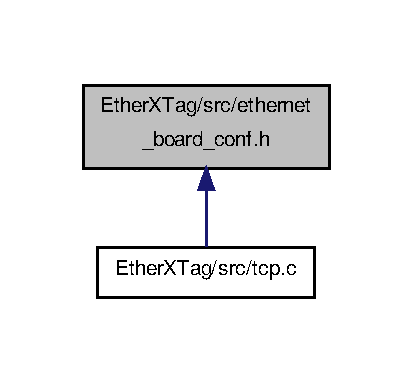
\includegraphics[width=198pt]{ethernet__board__conf_8h__dep__incl}
\end{center}
\end{figure}
\subsection*{Macros}
\begin{DoxyCompactItemize}
\item 
\#define \hyperlink{ethernet__board__conf_8h_ae3e2d8db2a681cd789f9a6e6e01ccc81}{E\-T\-H\-E\-R\-N\-E\-T\-\_\-\-D\-E\-F\-A\-U\-L\-T\-\_\-\-P\-H\-Y\-\_\-\-A\-D\-D\-R\-E\-S\-S}~0
\item 
\#define \hyperlink{ethernet__board__conf_8h_a589d6639a5626da2417c0cdcd31c2d96}{E\-T\-H\-E\-R\-N\-E\-T\-\_\-\-D\-E\-F\-A\-U\-L\-T\-\_\-\-T\-I\-L\-E}~tile\mbox{[}0\mbox{]}
\item 
\#define \hyperlink{ethernet__board__conf_8h_aaf14e6a6d195384bcd247526c58d27b4}{P\-O\-R\-T\-\_\-\-E\-T\-H\-\_\-\-R\-X\-C\-L\-K}~on tile\mbox{[}0\mbox{]}\-: X\-S1\-\_\-\-P\-O\-R\-T\-\_\-1\-J
\item 
\#define \hyperlink{ethernet__board__conf_8h_a786ed2869a88846791066f609c2f9beb}{P\-O\-R\-T\-\_\-\-E\-T\-H\-\_\-\-R\-X\-D}~on tile\mbox{[}0\mbox{]}\-: X\-S1\-\_\-\-P\-O\-R\-T\-\_\-4\-C
\item 
\#define \hyperlink{ethernet__board__conf_8h_a462e7f846c763133aeef597e2bf7a863}{P\-O\-R\-T\-\_\-\-E\-T\-H\-\_\-\-T\-X\-D}~on tile\mbox{[}0\mbox{]}\-: X\-S1\-\_\-\-P\-O\-R\-T\-\_\-4\-D
\item 
\#define \hyperlink{ethernet__board__conf_8h_aa2152ed230ba0301cebf5dcb26914271}{P\-O\-R\-T\-\_\-\-E\-T\-H\-\_\-\-R\-X\-D\-V}~on tile\mbox{[}0\mbox{]}\-: X\-S1\-\_\-\-P\-O\-R\-T\-\_\-1\-K
\item 
\#define \hyperlink{ethernet__board__conf_8h_ac94c0d25cae0e79f3a55e15bae3872cd}{P\-O\-R\-T\-\_\-\-E\-T\-H\-\_\-\-T\-X\-E\-N}~on tile\mbox{[}0\mbox{]}\-: X\-S1\-\_\-\-P\-O\-R\-T\-\_\-1\-L
\item 
\#define \hyperlink{ethernet__board__conf_8h_a8256b37a26beace7b9a4fb3b761463a7}{P\-O\-R\-T\-\_\-\-E\-T\-H\-\_\-\-T\-X\-C\-L\-K}~on tile\mbox{[}0\mbox{]}\-: X\-S1\-\_\-\-P\-O\-R\-T\-\_\-1\-I
\item 
\#define \hyperlink{ethernet__board__conf_8h_a6439d941e44e6860231a308ab5459d1b}{P\-O\-R\-T\-\_\-\-E\-T\-H\-\_\-\-M\-D\-I\-O}~on tile\mbox{[}0\mbox{]}\-: X\-S1\-\_\-\-P\-O\-R\-T\-\_\-1\-M
\item 
\#define \hyperlink{ethernet__board__conf_8h_a6ed64194bb42b032db2ca0357d6ed472}{P\-O\-R\-T\-\_\-\-E\-T\-H\-\_\-\-M\-D\-C}~on tile\mbox{[}0\mbox{]}\-: X\-S1\-\_\-\-P\-O\-R\-T\-\_\-1\-N
\item 
\#define \hyperlink{ethernet__board__conf_8h_a9fc7341562a703a1964e65185aa881e8}{P\-O\-R\-T\-\_\-\-E\-T\-H\-\_\-\-I\-N\-T}~on tile\mbox{[}0\mbox{]}\-: X\-S1\-\_\-\-P\-O\-R\-T\-\_\-1\-O
\item 
\#define \hyperlink{ethernet__board__conf_8h_aa3e3dd54fb0433921db1e112f338cbf0}{P\-O\-R\-T\-\_\-\-E\-T\-H\-\_\-\-E\-R\-R}~on tile\mbox{[}0\mbox{]}\-: X\-S1\-\_\-\-P\-O\-R\-T\-\_\-1\-P
\end{DoxyCompactItemize}


\subsection{Macro Definition Documentation}
\hypertarget{ethernet__board__conf_8h_ae3e2d8db2a681cd789f9a6e6e01ccc81}{\index{ethernet\-\_\-board\-\_\-conf.\-h@{ethernet\-\_\-board\-\_\-conf.\-h}!E\-T\-H\-E\-R\-N\-E\-T\-\_\-\-D\-E\-F\-A\-U\-L\-T\-\_\-\-P\-H\-Y\-\_\-\-A\-D\-D\-R\-E\-S\-S@{E\-T\-H\-E\-R\-N\-E\-T\-\_\-\-D\-E\-F\-A\-U\-L\-T\-\_\-\-P\-H\-Y\-\_\-\-A\-D\-D\-R\-E\-S\-S}}
\index{E\-T\-H\-E\-R\-N\-E\-T\-\_\-\-D\-E\-F\-A\-U\-L\-T\-\_\-\-P\-H\-Y\-\_\-\-A\-D\-D\-R\-E\-S\-S@{E\-T\-H\-E\-R\-N\-E\-T\-\_\-\-D\-E\-F\-A\-U\-L\-T\-\_\-\-P\-H\-Y\-\_\-\-A\-D\-D\-R\-E\-S\-S}!ethernet_board_conf.h@{ethernet\-\_\-board\-\_\-conf.\-h}}
\subsubsection[{E\-T\-H\-E\-R\-N\-E\-T\-\_\-\-D\-E\-F\-A\-U\-L\-T\-\_\-\-P\-H\-Y\-\_\-\-A\-D\-D\-R\-E\-S\-S}]{\setlength{\rightskip}{0pt plus 5cm}\#define E\-T\-H\-E\-R\-N\-E\-T\-\_\-\-D\-E\-F\-A\-U\-L\-T\-\_\-\-P\-H\-Y\-\_\-\-A\-D\-D\-R\-E\-S\-S~0}}\label{ethernet__board__conf_8h_ae3e2d8db2a681cd789f9a6e6e01ccc81}


Definition at line 8 of file ethernet\-\_\-board\-\_\-conf.\-h.

\hypertarget{ethernet__board__conf_8h_a589d6639a5626da2417c0cdcd31c2d96}{\index{ethernet\-\_\-board\-\_\-conf.\-h@{ethernet\-\_\-board\-\_\-conf.\-h}!E\-T\-H\-E\-R\-N\-E\-T\-\_\-\-D\-E\-F\-A\-U\-L\-T\-\_\-\-T\-I\-L\-E@{E\-T\-H\-E\-R\-N\-E\-T\-\_\-\-D\-E\-F\-A\-U\-L\-T\-\_\-\-T\-I\-L\-E}}
\index{E\-T\-H\-E\-R\-N\-E\-T\-\_\-\-D\-E\-F\-A\-U\-L\-T\-\_\-\-T\-I\-L\-E@{E\-T\-H\-E\-R\-N\-E\-T\-\_\-\-D\-E\-F\-A\-U\-L\-T\-\_\-\-T\-I\-L\-E}!ethernet_board_conf.h@{ethernet\-\_\-board\-\_\-conf.\-h}}
\subsubsection[{E\-T\-H\-E\-R\-N\-E\-T\-\_\-\-D\-E\-F\-A\-U\-L\-T\-\_\-\-T\-I\-L\-E}]{\setlength{\rightskip}{0pt plus 5cm}\#define E\-T\-H\-E\-R\-N\-E\-T\-\_\-\-D\-E\-F\-A\-U\-L\-T\-\_\-\-T\-I\-L\-E~tile\mbox{[}0\mbox{]}}}\label{ethernet__board__conf_8h_a589d6639a5626da2417c0cdcd31c2d96}


Definition at line 75 of file ethernet\-\_\-board\-\_\-conf.\-h.

\hypertarget{ethernet__board__conf_8h_aa3e3dd54fb0433921db1e112f338cbf0}{\index{ethernet\-\_\-board\-\_\-conf.\-h@{ethernet\-\_\-board\-\_\-conf.\-h}!P\-O\-R\-T\-\_\-\-E\-T\-H\-\_\-\-E\-R\-R@{P\-O\-R\-T\-\_\-\-E\-T\-H\-\_\-\-E\-R\-R}}
\index{P\-O\-R\-T\-\_\-\-E\-T\-H\-\_\-\-E\-R\-R@{P\-O\-R\-T\-\_\-\-E\-T\-H\-\_\-\-E\-R\-R}!ethernet_board_conf.h@{ethernet\-\_\-board\-\_\-conf.\-h}}
\subsubsection[{P\-O\-R\-T\-\_\-\-E\-T\-H\-\_\-\-E\-R\-R}]{\setlength{\rightskip}{0pt plus 5cm}\#define P\-O\-R\-T\-\_\-\-E\-T\-H\-\_\-\-E\-R\-R~on tile\mbox{[}0\mbox{]}\-: X\-S1\-\_\-\-P\-O\-R\-T\-\_\-1\-P}}\label{ethernet__board__conf_8h_aa3e3dd54fb0433921db1e112f338cbf0}


Definition at line 85 of file ethernet\-\_\-board\-\_\-conf.\-h.

\hypertarget{ethernet__board__conf_8h_a9fc7341562a703a1964e65185aa881e8}{\index{ethernet\-\_\-board\-\_\-conf.\-h@{ethernet\-\_\-board\-\_\-conf.\-h}!P\-O\-R\-T\-\_\-\-E\-T\-H\-\_\-\-I\-N\-T@{P\-O\-R\-T\-\_\-\-E\-T\-H\-\_\-\-I\-N\-T}}
\index{P\-O\-R\-T\-\_\-\-E\-T\-H\-\_\-\-I\-N\-T@{P\-O\-R\-T\-\_\-\-E\-T\-H\-\_\-\-I\-N\-T}!ethernet_board_conf.h@{ethernet\-\_\-board\-\_\-conf.\-h}}
\subsubsection[{P\-O\-R\-T\-\_\-\-E\-T\-H\-\_\-\-I\-N\-T}]{\setlength{\rightskip}{0pt plus 5cm}\#define P\-O\-R\-T\-\_\-\-E\-T\-H\-\_\-\-I\-N\-T~on tile\mbox{[}0\mbox{]}\-: X\-S1\-\_\-\-P\-O\-R\-T\-\_\-1\-O}}\label{ethernet__board__conf_8h_a9fc7341562a703a1964e65185aa881e8}


Definition at line 84 of file ethernet\-\_\-board\-\_\-conf.\-h.

\hypertarget{ethernet__board__conf_8h_a6ed64194bb42b032db2ca0357d6ed472}{\index{ethernet\-\_\-board\-\_\-conf.\-h@{ethernet\-\_\-board\-\_\-conf.\-h}!P\-O\-R\-T\-\_\-\-E\-T\-H\-\_\-\-M\-D\-C@{P\-O\-R\-T\-\_\-\-E\-T\-H\-\_\-\-M\-D\-C}}
\index{P\-O\-R\-T\-\_\-\-E\-T\-H\-\_\-\-M\-D\-C@{P\-O\-R\-T\-\_\-\-E\-T\-H\-\_\-\-M\-D\-C}!ethernet_board_conf.h@{ethernet\-\_\-board\-\_\-conf.\-h}}
\subsubsection[{P\-O\-R\-T\-\_\-\-E\-T\-H\-\_\-\-M\-D\-C}]{\setlength{\rightskip}{0pt plus 5cm}\#define P\-O\-R\-T\-\_\-\-E\-T\-H\-\_\-\-M\-D\-C~on tile\mbox{[}0\mbox{]}\-: X\-S1\-\_\-\-P\-O\-R\-T\-\_\-1\-N}}\label{ethernet__board__conf_8h_a6ed64194bb42b032db2ca0357d6ed472}


Definition at line 83 of file ethernet\-\_\-board\-\_\-conf.\-h.

\hypertarget{ethernet__board__conf_8h_a6439d941e44e6860231a308ab5459d1b}{\index{ethernet\-\_\-board\-\_\-conf.\-h@{ethernet\-\_\-board\-\_\-conf.\-h}!P\-O\-R\-T\-\_\-\-E\-T\-H\-\_\-\-M\-D\-I\-O@{P\-O\-R\-T\-\_\-\-E\-T\-H\-\_\-\-M\-D\-I\-O}}
\index{P\-O\-R\-T\-\_\-\-E\-T\-H\-\_\-\-M\-D\-I\-O@{P\-O\-R\-T\-\_\-\-E\-T\-H\-\_\-\-M\-D\-I\-O}!ethernet_board_conf.h@{ethernet\-\_\-board\-\_\-conf.\-h}}
\subsubsection[{P\-O\-R\-T\-\_\-\-E\-T\-H\-\_\-\-M\-D\-I\-O}]{\setlength{\rightskip}{0pt plus 5cm}\#define P\-O\-R\-T\-\_\-\-E\-T\-H\-\_\-\-M\-D\-I\-O~on tile\mbox{[}0\mbox{]}\-: X\-S1\-\_\-\-P\-O\-R\-T\-\_\-1\-M}}\label{ethernet__board__conf_8h_a6439d941e44e6860231a308ab5459d1b}


Definition at line 82 of file ethernet\-\_\-board\-\_\-conf.\-h.

\hypertarget{ethernet__board__conf_8h_aaf14e6a6d195384bcd247526c58d27b4}{\index{ethernet\-\_\-board\-\_\-conf.\-h@{ethernet\-\_\-board\-\_\-conf.\-h}!P\-O\-R\-T\-\_\-\-E\-T\-H\-\_\-\-R\-X\-C\-L\-K@{P\-O\-R\-T\-\_\-\-E\-T\-H\-\_\-\-R\-X\-C\-L\-K}}
\index{P\-O\-R\-T\-\_\-\-E\-T\-H\-\_\-\-R\-X\-C\-L\-K@{P\-O\-R\-T\-\_\-\-E\-T\-H\-\_\-\-R\-X\-C\-L\-K}!ethernet_board_conf.h@{ethernet\-\_\-board\-\_\-conf.\-h}}
\subsubsection[{P\-O\-R\-T\-\_\-\-E\-T\-H\-\_\-\-R\-X\-C\-L\-K}]{\setlength{\rightskip}{0pt plus 5cm}\#define P\-O\-R\-T\-\_\-\-E\-T\-H\-\_\-\-R\-X\-C\-L\-K~on tile\mbox{[}0\mbox{]}\-: X\-S1\-\_\-\-P\-O\-R\-T\-\_\-1\-J}}\label{ethernet__board__conf_8h_aaf14e6a6d195384bcd247526c58d27b4}


Definition at line 76 of file ethernet\-\_\-board\-\_\-conf.\-h.

\hypertarget{ethernet__board__conf_8h_a786ed2869a88846791066f609c2f9beb}{\index{ethernet\-\_\-board\-\_\-conf.\-h@{ethernet\-\_\-board\-\_\-conf.\-h}!P\-O\-R\-T\-\_\-\-E\-T\-H\-\_\-\-R\-X\-D@{P\-O\-R\-T\-\_\-\-E\-T\-H\-\_\-\-R\-X\-D}}
\index{P\-O\-R\-T\-\_\-\-E\-T\-H\-\_\-\-R\-X\-D@{P\-O\-R\-T\-\_\-\-E\-T\-H\-\_\-\-R\-X\-D}!ethernet_board_conf.h@{ethernet\-\_\-board\-\_\-conf.\-h}}
\subsubsection[{P\-O\-R\-T\-\_\-\-E\-T\-H\-\_\-\-R\-X\-D}]{\setlength{\rightskip}{0pt plus 5cm}\#define P\-O\-R\-T\-\_\-\-E\-T\-H\-\_\-\-R\-X\-D~on tile\mbox{[}0\mbox{]}\-: X\-S1\-\_\-\-P\-O\-R\-T\-\_\-4\-C}}\label{ethernet__board__conf_8h_a786ed2869a88846791066f609c2f9beb}


Definition at line 77 of file ethernet\-\_\-board\-\_\-conf.\-h.

\hypertarget{ethernet__board__conf_8h_aa2152ed230ba0301cebf5dcb26914271}{\index{ethernet\-\_\-board\-\_\-conf.\-h@{ethernet\-\_\-board\-\_\-conf.\-h}!P\-O\-R\-T\-\_\-\-E\-T\-H\-\_\-\-R\-X\-D\-V@{P\-O\-R\-T\-\_\-\-E\-T\-H\-\_\-\-R\-X\-D\-V}}
\index{P\-O\-R\-T\-\_\-\-E\-T\-H\-\_\-\-R\-X\-D\-V@{P\-O\-R\-T\-\_\-\-E\-T\-H\-\_\-\-R\-X\-D\-V}!ethernet_board_conf.h@{ethernet\-\_\-board\-\_\-conf.\-h}}
\subsubsection[{P\-O\-R\-T\-\_\-\-E\-T\-H\-\_\-\-R\-X\-D\-V}]{\setlength{\rightskip}{0pt plus 5cm}\#define P\-O\-R\-T\-\_\-\-E\-T\-H\-\_\-\-R\-X\-D\-V~on tile\mbox{[}0\mbox{]}\-: X\-S1\-\_\-\-P\-O\-R\-T\-\_\-1\-K}}\label{ethernet__board__conf_8h_aa2152ed230ba0301cebf5dcb26914271}


Definition at line 79 of file ethernet\-\_\-board\-\_\-conf.\-h.

\hypertarget{ethernet__board__conf_8h_a8256b37a26beace7b9a4fb3b761463a7}{\index{ethernet\-\_\-board\-\_\-conf.\-h@{ethernet\-\_\-board\-\_\-conf.\-h}!P\-O\-R\-T\-\_\-\-E\-T\-H\-\_\-\-T\-X\-C\-L\-K@{P\-O\-R\-T\-\_\-\-E\-T\-H\-\_\-\-T\-X\-C\-L\-K}}
\index{P\-O\-R\-T\-\_\-\-E\-T\-H\-\_\-\-T\-X\-C\-L\-K@{P\-O\-R\-T\-\_\-\-E\-T\-H\-\_\-\-T\-X\-C\-L\-K}!ethernet_board_conf.h@{ethernet\-\_\-board\-\_\-conf.\-h}}
\subsubsection[{P\-O\-R\-T\-\_\-\-E\-T\-H\-\_\-\-T\-X\-C\-L\-K}]{\setlength{\rightskip}{0pt plus 5cm}\#define P\-O\-R\-T\-\_\-\-E\-T\-H\-\_\-\-T\-X\-C\-L\-K~on tile\mbox{[}0\mbox{]}\-: X\-S1\-\_\-\-P\-O\-R\-T\-\_\-1\-I}}\label{ethernet__board__conf_8h_a8256b37a26beace7b9a4fb3b761463a7}


Definition at line 81 of file ethernet\-\_\-board\-\_\-conf.\-h.

\hypertarget{ethernet__board__conf_8h_a462e7f846c763133aeef597e2bf7a863}{\index{ethernet\-\_\-board\-\_\-conf.\-h@{ethernet\-\_\-board\-\_\-conf.\-h}!P\-O\-R\-T\-\_\-\-E\-T\-H\-\_\-\-T\-X\-D@{P\-O\-R\-T\-\_\-\-E\-T\-H\-\_\-\-T\-X\-D}}
\index{P\-O\-R\-T\-\_\-\-E\-T\-H\-\_\-\-T\-X\-D@{P\-O\-R\-T\-\_\-\-E\-T\-H\-\_\-\-T\-X\-D}!ethernet_board_conf.h@{ethernet\-\_\-board\-\_\-conf.\-h}}
\subsubsection[{P\-O\-R\-T\-\_\-\-E\-T\-H\-\_\-\-T\-X\-D}]{\setlength{\rightskip}{0pt plus 5cm}\#define P\-O\-R\-T\-\_\-\-E\-T\-H\-\_\-\-T\-X\-D~on tile\mbox{[}0\mbox{]}\-: X\-S1\-\_\-\-P\-O\-R\-T\-\_\-4\-D}}\label{ethernet__board__conf_8h_a462e7f846c763133aeef597e2bf7a863}


Definition at line 78 of file ethernet\-\_\-board\-\_\-conf.\-h.

\hypertarget{ethernet__board__conf_8h_ac94c0d25cae0e79f3a55e15bae3872cd}{\index{ethernet\-\_\-board\-\_\-conf.\-h@{ethernet\-\_\-board\-\_\-conf.\-h}!P\-O\-R\-T\-\_\-\-E\-T\-H\-\_\-\-T\-X\-E\-N@{P\-O\-R\-T\-\_\-\-E\-T\-H\-\_\-\-T\-X\-E\-N}}
\index{P\-O\-R\-T\-\_\-\-E\-T\-H\-\_\-\-T\-X\-E\-N@{P\-O\-R\-T\-\_\-\-E\-T\-H\-\_\-\-T\-X\-E\-N}!ethernet_board_conf.h@{ethernet\-\_\-board\-\_\-conf.\-h}}
\subsubsection[{P\-O\-R\-T\-\_\-\-E\-T\-H\-\_\-\-T\-X\-E\-N}]{\setlength{\rightskip}{0pt plus 5cm}\#define P\-O\-R\-T\-\_\-\-E\-T\-H\-\_\-\-T\-X\-E\-N~on tile\mbox{[}0\mbox{]}\-: X\-S1\-\_\-\-P\-O\-R\-T\-\_\-1\-L}}\label{ethernet__board__conf_8h_ac94c0d25cae0e79f3a55e15bae3872cd}


Definition at line 80 of file ethernet\-\_\-board\-\_\-conf.\-h.


\hypertarget{mdns_8c}{\section{Ether\-X\-Tag/src/mdns.c File Reference}
\label{mdns_8c}\index{Ether\-X\-Tag/src/mdns.\-c@{Ether\-X\-Tag/src/mdns.\-c}}
}
{\ttfamily \#include $<$assert.\-h$>$}\\*
{\ttfamily \#include $<$string.\-h$>$}\\*
{\ttfamily \#include \char`\"{}mdns.\-h\char`\"{}}\\*
Include dependency graph for mdns.\-c\-:\nopagebreak
\begin{figure}[H]
\begin{center}
\leavevmode
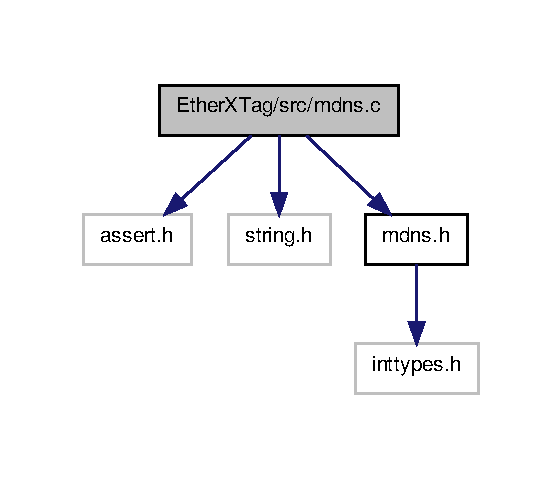
\includegraphics[width=269pt]{mdns_8c__incl}
\end{center}
\end{figure}
\subsection*{Functions}
\begin{DoxyCompactItemize}
\item 
void \hyperlink{mdns_8c_af566bde7a173589ff6c55e76e3c2ccc2}{encode\-\_\-packet} (\hyperlink{structdns__packet__t}{dns\-\_\-packet\-\_\-t} $\ast$pkt, char $\ast$buffer, int len)
\begin{DoxyCompactList}\small\item\em Encode a packet into a buffer for transmission on a network. \end{DoxyCompactList}\item 
\hyperlink{structdns__packet__t}{dns\-\_\-packet\-\_\-t} \hyperlink{mdns_8c_adb6c64d79a5c3c6877820d9b4f924140}{decode\-\_\-packet} (char $\ast$buffer)
\begin{DoxyCompactList}\small\item\em Decode a packet from a buffer. \end{DoxyCompactList}\item 
int \hyperlink{mdns_8c_a99583e0d313be789aa2017d9490aa024}{count\-\_\-packet\-\_\-length} (\hyperlink{structdns__packet__t}{dns\-\_\-packet\-\_\-t} $\ast$pkt)
\begin{DoxyCompactList}\small\item\em returns the length of a packet \end{DoxyCompactList}\item 
uint16\-\_\-t \hyperlink{mdns_8c_af792d74a36744bbc7307fd9a7dedd234}{ntohs} (uint16\-\_\-t val)
\begin{DoxyCompactList}\small\item\em Swap the endianness of a short value. \end{DoxyCompactList}\item 
void \hyperlink{mdns_8c_afbd495d1272cd02c84e44c681dd08671}{correct\-\_\-header\-\_\-endianness} (\hyperlink{structdns__packet__header__t}{dns\-\_\-packet\-\_\-header\-\_\-t} $\ast$pkt)
\begin{DoxyCompactList}\small\item\em Corrects the endiannes of data in a D\-N\-S packet header. \end{DoxyCompactList}\item 
void \hyperlink{mdns_8c_af345abaecbfbfc2b7070d55e377dc08c}{correct\-\_\-endianness} (\hyperlink{structdns__packet__t}{dns\-\_\-packet\-\_\-t} $\ast$pkt)
\begin{DoxyCompactList}\small\item\em Corrects the endianness of data in a D\-N\-S packet. \end{DoxyCompactList}\end{DoxyCompactItemize}


\subsection{Function Documentation}
\hypertarget{mdns_8c_af345abaecbfbfc2b7070d55e377dc08c}{\index{mdns.\-c@{mdns.\-c}!correct\-\_\-endianness@{correct\-\_\-endianness}}
\index{correct\-\_\-endianness@{correct\-\_\-endianness}!mdns.c@{mdns.\-c}}
\subsubsection[{correct\-\_\-endianness}]{\setlength{\rightskip}{0pt plus 5cm}void correct\-\_\-endianness (
\begin{DoxyParamCaption}
\item[{{\bf dns\-\_\-packet\-\_\-t} $\ast$}]{pkt}
\end{DoxyParamCaption}
)}}\label{mdns_8c_af345abaecbfbfc2b7070d55e377dc08c}


Corrects the endianness of data in a D\-N\-S packet. 

A\-R\-P\-A defines internet trafic to be big endian, but most machines now are little endian, so this function corrects that for relevant parts of a packet. 

Definition at line 122 of file mdns.\-c.

\hypertarget{mdns_8c_afbd495d1272cd02c84e44c681dd08671}{\index{mdns.\-c@{mdns.\-c}!correct\-\_\-header\-\_\-endianness@{correct\-\_\-header\-\_\-endianness}}
\index{correct\-\_\-header\-\_\-endianness@{correct\-\_\-header\-\_\-endianness}!mdns.c@{mdns.\-c}}
\subsubsection[{correct\-\_\-header\-\_\-endianness}]{\setlength{\rightskip}{0pt plus 5cm}void correct\-\_\-header\-\_\-endianness (
\begin{DoxyParamCaption}
\item[{{\bf dns\-\_\-packet\-\_\-header\-\_\-t} $\ast$}]{pkt}
\end{DoxyParamCaption}
)}}\label{mdns_8c_afbd495d1272cd02c84e44c681dd08671}


Corrects the endiannes of data in a D\-N\-S packet header. 

A\-R\-P\-A defines internet trafic to be big endian, but most machines now are little endian, so this function corrects that for relevant parts of a packet. 

Definition at line 113 of file mdns.\-c.

\hypertarget{mdns_8c_a99583e0d313be789aa2017d9490aa024}{\index{mdns.\-c@{mdns.\-c}!count\-\_\-packet\-\_\-length@{count\-\_\-packet\-\_\-length}}
\index{count\-\_\-packet\-\_\-length@{count\-\_\-packet\-\_\-length}!mdns.c@{mdns.\-c}}
\subsubsection[{count\-\_\-packet\-\_\-length}]{\setlength{\rightskip}{0pt plus 5cm}int count\-\_\-packet\-\_\-length (
\begin{DoxyParamCaption}
\item[{{\bf dns\-\_\-packet\-\_\-t} $\ast$}]{pkt}
\end{DoxyParamCaption}
)}}\label{mdns_8c_a99583e0d313be789aa2017d9490aa024}


returns the length of a packet 

returns the total length of a packet, including it's header and payload. 

Definition at line 94 of file mdns.\-c.

\hypertarget{mdns_8c_adb6c64d79a5c3c6877820d9b4f924140}{\index{mdns.\-c@{mdns.\-c}!decode\-\_\-packet@{decode\-\_\-packet}}
\index{decode\-\_\-packet@{decode\-\_\-packet}!mdns.c@{mdns.\-c}}
\subsubsection[{decode\-\_\-packet}]{\setlength{\rightskip}{0pt plus 5cm}{\bf dns\-\_\-packet\-\_\-t} decode\-\_\-packet (
\begin{DoxyParamCaption}
\item[{char $\ast$}]{buffer}
\end{DoxyParamCaption}
)}}\label{mdns_8c_adb6c64d79a5c3c6877820d9b4f924140}


Decode a packet from a buffer. 

Read out a buffer, e.\-g. read from a network, and fill a \hyperlink{structdns__packet__t}{dns\-\_\-packet\-\_\-t} object. 

Definition at line 41 of file mdns.\-c.

\hypertarget{mdns_8c_af566bde7a173589ff6c55e76e3c2ccc2}{\index{mdns.\-c@{mdns.\-c}!encode\-\_\-packet@{encode\-\_\-packet}}
\index{encode\-\_\-packet@{encode\-\_\-packet}!mdns.c@{mdns.\-c}}
\subsubsection[{encode\-\_\-packet}]{\setlength{\rightskip}{0pt plus 5cm}void encode\-\_\-packet (
\begin{DoxyParamCaption}
\item[{{\bf dns\-\_\-packet\-\_\-t} $\ast$}]{pkt, }
\item[{char $\ast$}]{buffer, }
\item[{int}]{len}
\end{DoxyParamCaption}
)}}\label{mdns_8c_af566bde7a173589ff6c55e76e3c2ccc2}


Encode a packet into a buffer for transmission on a network. 

A super simple implementation of M\-D\-N\-S for the X\-Core. 

Definition at line 9 of file mdns.\-c.

\hypertarget{mdns_8c_af792d74a36744bbc7307fd9a7dedd234}{\index{mdns.\-c@{mdns.\-c}!ntohs@{ntohs}}
\index{ntohs@{ntohs}!mdns.c@{mdns.\-c}}
\subsubsection[{ntohs}]{\setlength{\rightskip}{0pt plus 5cm}uint16\-\_\-t ntohs (
\begin{DoxyParamCaption}
\item[{uint16\-\_\-t}]{val}
\end{DoxyParamCaption}
)}}\label{mdns_8c_af792d74a36744bbc7307fd9a7dedd234}


Swap the endianness of a short value. 

Swap the upper and lower octets of a 2 byte value. 

Definition at line 108 of file mdns.\-c.


\hypertarget{mdns_8h}{\section{Ether\-X\-Tag/src/mdns.h File Reference}
\label{mdns_8h}\index{Ether\-X\-Tag/src/mdns.\-h@{Ether\-X\-Tag/src/mdns.\-h}}
}
{\ttfamily \#include $<$inttypes.\-h$>$}\\*
Include dependency graph for mdns.\-h\-:\nopagebreak
\begin{figure}[H]
\begin{center}
\leavevmode
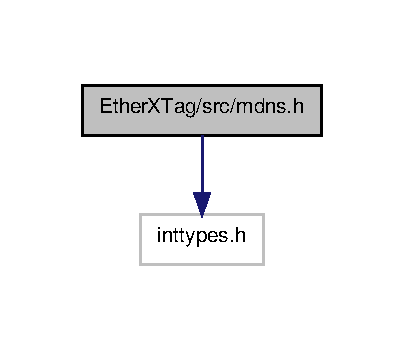
\includegraphics[width=194pt]{mdns_8h__incl}
\end{center}
\end{figure}
This graph shows which files directly or indirectly include this file\-:\nopagebreak
\begin{figure}[H]
\begin{center}
\leavevmode
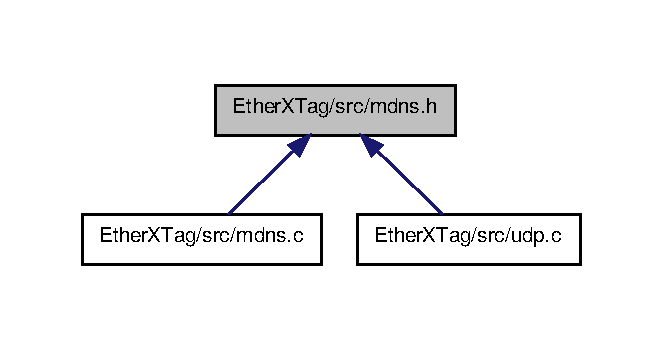
\includegraphics[width=318pt]{mdns_8h__dep__incl}
\end{center}
\end{figure}
\subsection*{Data Structures}
\begin{DoxyCompactItemize}
\item 
struct \hyperlink{structdns__flags__t}{dns\-\_\-flags\-\_\-t}
\item 
struct \hyperlink{structdns__packet__header__t}{dns\-\_\-packet\-\_\-header\-\_\-t}
\begin{DoxyCompactList}\small\item\em D\-N\-S Packet header. \end{DoxyCompactList}\item 
struct \hyperlink{structdns__packet__t}{dns\-\_\-packet\-\_\-t}
\begin{DoxyCompactList}\small\item\em D\-N\-S Packet. \end{DoxyCompactList}\end{DoxyCompactItemize}
\subsection*{Macros}
\begin{DoxyCompactItemize}
\item 
\#define \hyperlink{mdns_8h_a4b8c161f7a3f996f5f092bf869448c8a}{S\-I\-Z\-E\-\_\-\-O\-F\-\_\-\-D\-N\-S\-\_\-\-H\-E\-A\-D\-E\-R}~12
\end{DoxyCompactItemize}
\subsection*{Typedefs}
\begin{DoxyCompactItemize}
\item 
typedef struct \hyperlink{structdns__flags__t}{dns\-\_\-flags\-\_\-t} \hyperlink{mdns_8h_a1461793344892bd3a6bfc0946d7d81aa}{dns\-\_\-flags\-\_\-t}
\item 
typedef struct \hyperlink{structdns__packet__header__t}{dns\-\_\-packet\-\_\-header\-\_\-t} \hyperlink{mdns_8h_a1d8d1a66bfe0cc2f47340bcf00f3584c}{dns\-\_\-packet\-\_\-header\-\_\-t}
\begin{DoxyCompactList}\small\item\em D\-N\-S Packet header. \end{DoxyCompactList}\item 
typedef struct \hyperlink{structdns__packet__t}{dns\-\_\-packet\-\_\-t} \hyperlink{mdns_8h_afa145699b23a8a07d5ffda178e09622b}{dns\-\_\-packet\-\_\-t}
\begin{DoxyCompactList}\small\item\em D\-N\-S Packet. \end{DoxyCompactList}\end{DoxyCompactItemize}
\subsection*{Enumerations}
\begin{DoxyCompactItemize}
\item 
enum \hyperlink{mdns_8h_af9eceef222a0a264c35b898ae133e2a2}{D\-N\-S\-\_\-\-R\-E\-T\-U\-R\-N\-\_\-\-C\-O\-D\-E} \{ \\*
\hyperlink{mdns_8h_af9eceef222a0a264c35b898ae133e2a2ab46046c86c89a9df5a4ac6bf82bba011}{D\-N\-S\-\_\-\-N\-O\-\_\-\-E\-R\-R\-O\-R} =  0, 
\hyperlink{mdns_8h_af9eceef222a0a264c35b898ae133e2a2a17caf088a135ba3c185987510a5bc458}{D\-N\-S\-\_\-\-F\-O\-R\-M\-A\-T\-\_\-\-E\-R\-R\-O\-R} =  1, 
\hyperlink{mdns_8h_af9eceef222a0a264c35b898ae133e2a2a556287473e158a5ebc5ae6af3eb6538a}{D\-N\-S\-\_\-\-S\-E\-R\-V\-E\-R\-\_\-\-F\-A\-I\-L} =  2, 
\hyperlink{mdns_8h_af9eceef222a0a264c35b898ae133e2a2a28bd8dcc0f084c630d5427ed7e612469}{D\-N\-S\-\_\-\-N\-A\-M\-E\-\_\-\-E\-R\-R\-O\-R} =  3, 
\\*
\hyperlink{mdns_8h_af9eceef222a0a264c35b898ae133e2a2a63972833cdcd983952b950df05edfdee}{D\-N\-S\-\_\-\-N\-O\-T\-\_\-\-I\-M\-P\-L\-E\-M\-E\-N\-T\-E\-D} =  4, 
\hyperlink{mdns_8h_af9eceef222a0a264c35b898ae133e2a2a1f60b454354158945846c9202f6d4074}{D\-N\-S\-\_\-\-R\-E\-F\-U\-S\-E\-D} =  5, 
\hyperlink{mdns_8h_af9eceef222a0a264c35b898ae133e2a2a80b660f8e6125b68cee1b5b8d4f826a6}{D\-N\-S\-\_\-\-Y\-X\-\_\-\-D\-O\-M\-A\-I\-N} =  6, 
\hyperlink{mdns_8h_af9eceef222a0a264c35b898ae133e2a2a12785854e261e7d5b34aa07fec888d3d}{D\-N\-S\-\_\-\-Y\-X\-\_\-\-R\-R\-\_\-\-S\-E\-T} =  7, 
\\*
\hyperlink{mdns_8h_af9eceef222a0a264c35b898ae133e2a2aa9e9159cceb081eb1357332e3767504b}{D\-N\-S\-\_\-\-N\-X\-\_\-\-R\-R\-\_\-\-S\-E\-T} =  8, 
\hyperlink{mdns_8h_af9eceef222a0a264c35b898ae133e2a2ad78c13d9ef851562cf7fc7faac755192}{D\-N\-S\-\_\-\-N\-O\-T\-\_\-\-A\-U\-T\-H\-O\-R\-I\-T\-A\-T\-I\-V\-E} =  9, 
\hyperlink{mdns_8h_af9eceef222a0a264c35b898ae133e2a2aa6c8976d60d8a52711a8971cee718578}{D\-N\-S\-\_\-\-N\-O\-T\-\_\-\-Z\-O\-N\-E} =  10, 
\hyperlink{mdns_8h_af9eceef222a0a264c35b898ae133e2a2a791f90670074a7fd48d66d3b9e621023}{D\-N\-S\-\_\-\-B\-A\-D\-\_\-\-V\-E\-R\-S} =  16, 
\\*
\hyperlink{mdns_8h_af9eceef222a0a264c35b898ae133e2a2a64848d381348c73438676ddefb9724e2}{D\-N\-S\-\_\-\-B\-A\-D\-\_\-\-K\-E\-Y} =  17, 
\hyperlink{mdns_8h_af9eceef222a0a264c35b898ae133e2a2a974c103170362252a16b62f4a463a256}{D\-N\-S\-\_\-\-B\-A\-D\-\_\-\-T\-I\-M\-E} =  18, 
\hyperlink{mdns_8h_af9eceef222a0a264c35b898ae133e2a2ada35f3bf681d66623ab4e271f7ec2913}{D\-N\-S\-\_\-\-B\-A\-D\-\_\-\-M\-O\-D\-E} =  19, 
\hyperlink{mdns_8h_af9eceef222a0a264c35b898ae133e2a2a096b3433f20cf97d3fec679b882a50ec}{D\-N\-S\-\_\-\-B\-A\-D\-\_\-\-N\-A\-M\-E} =  20, 
\\*
\hyperlink{mdns_8h_af9eceef222a0a264c35b898ae133e2a2a6a196e2ea197c389dc35299f8aec3156}{D\-N\-S\-\_\-\-B\-A\-D\-\_\-\-A\-L\-G} =  21, 
\hyperlink{mdns_8h_af9eceef222a0a264c35b898ae133e2a2a7119ee984846eb81347d20abfd869d45}{D\-N\-S\-\_\-\-B\-A\-D\-\_\-\-T\-R\-U\-N\-C} =  22
 \}
\end{DoxyCompactItemize}
\subsection*{Functions}
\begin{DoxyCompactItemize}
\item 
int \hyperlink{mdns_8h_a99583e0d313be789aa2017d9490aa024}{count\-\_\-packet\-\_\-length} (\hyperlink{structdns__packet__t}{dns\-\_\-packet\-\_\-t} $\ast$pkt)
\begin{DoxyCompactList}\small\item\em returns the length of a packet \end{DoxyCompactList}\item 
void \hyperlink{mdns_8h_af345abaecbfbfc2b7070d55e377dc08c}{correct\-\_\-endianness} (\hyperlink{structdns__packet__t}{dns\-\_\-packet\-\_\-t} $\ast$pkt)
\begin{DoxyCompactList}\small\item\em Corrects the endianness of data in a D\-N\-S packet. \end{DoxyCompactList}\item 
void \hyperlink{mdns_8h_afbd495d1272cd02c84e44c681dd08671}{correct\-\_\-header\-\_\-endianness} (\hyperlink{structdns__packet__header__t}{dns\-\_\-packet\-\_\-header\-\_\-t} $\ast$pkt)
\begin{DoxyCompactList}\small\item\em Corrects the endiannes of data in a D\-N\-S packet header. \end{DoxyCompactList}\item 
void \hyperlink{mdns_8h_af566bde7a173589ff6c55e76e3c2ccc2}{encode\-\_\-packet} (\hyperlink{structdns__packet__t}{dns\-\_\-packet\-\_\-t} $\ast$pkt, char $\ast$buffer, int len)
\begin{DoxyCompactList}\small\item\em Encode a packet into a buffer for transmission on a network. \end{DoxyCompactList}\item 
\hyperlink{structdns__packet__t}{dns\-\_\-packet\-\_\-t} \hyperlink{mdns_8h_adb6c64d79a5c3c6877820d9b4f924140}{decode\-\_\-packet} (char $\ast$buffer)
\begin{DoxyCompactList}\small\item\em Decode a packet from a buffer. \end{DoxyCompactList}\item 
uint16\-\_\-t \hyperlink{mdns_8h_af792d74a36744bbc7307fd9a7dedd234}{ntohs} (uint16\-\_\-t val)
\begin{DoxyCompactList}\small\item\em Swap the endianness of a short value. \end{DoxyCompactList}\end{DoxyCompactItemize}


\subsection{Macro Definition Documentation}
\hypertarget{mdns_8h_a4b8c161f7a3f996f5f092bf869448c8a}{\index{mdns.\-h@{mdns.\-h}!S\-I\-Z\-E\-\_\-\-O\-F\-\_\-\-D\-N\-S\-\_\-\-H\-E\-A\-D\-E\-R@{S\-I\-Z\-E\-\_\-\-O\-F\-\_\-\-D\-N\-S\-\_\-\-H\-E\-A\-D\-E\-R}}
\index{S\-I\-Z\-E\-\_\-\-O\-F\-\_\-\-D\-N\-S\-\_\-\-H\-E\-A\-D\-E\-R@{S\-I\-Z\-E\-\_\-\-O\-F\-\_\-\-D\-N\-S\-\_\-\-H\-E\-A\-D\-E\-R}!mdns.h@{mdns.\-h}}
\subsubsection[{S\-I\-Z\-E\-\_\-\-O\-F\-\_\-\-D\-N\-S\-\_\-\-H\-E\-A\-D\-E\-R}]{\setlength{\rightskip}{0pt plus 5cm}\#define S\-I\-Z\-E\-\_\-\-O\-F\-\_\-\-D\-N\-S\-\_\-\-H\-E\-A\-D\-E\-R~12}}\label{mdns_8h_a4b8c161f7a3f996f5f092bf869448c8a}


Definition at line 6 of file mdns.\-h.



\subsection{Typedef Documentation}
\hypertarget{mdns_8h_a1461793344892bd3a6bfc0946d7d81aa}{\index{mdns.\-h@{mdns.\-h}!dns\-\_\-flags\-\_\-t@{dns\-\_\-flags\-\_\-t}}
\index{dns\-\_\-flags\-\_\-t@{dns\-\_\-flags\-\_\-t}!mdns.h@{mdns.\-h}}
\subsubsection[{dns\-\_\-flags\-\_\-t}]{\setlength{\rightskip}{0pt plus 5cm}typedef struct {\bf dns\-\_\-flags\-\_\-t}  {\bf dns\-\_\-flags\-\_\-t}}}\label{mdns_8h_a1461793344892bd3a6bfc0946d7d81aa}
\hypertarget{mdns_8h_a1d8d1a66bfe0cc2f47340bcf00f3584c}{\index{mdns.\-h@{mdns.\-h}!dns\-\_\-packet\-\_\-header\-\_\-t@{dns\-\_\-packet\-\_\-header\-\_\-t}}
\index{dns\-\_\-packet\-\_\-header\-\_\-t@{dns\-\_\-packet\-\_\-header\-\_\-t}!mdns.h@{mdns.\-h}}
\subsubsection[{dns\-\_\-packet\-\_\-header\-\_\-t}]{\setlength{\rightskip}{0pt plus 5cm}typedef struct {\bf dns\-\_\-packet\-\_\-header\-\_\-t}  {\bf dns\-\_\-packet\-\_\-header\-\_\-t}}}\label{mdns_8h_a1d8d1a66bfe0cc2f47340bcf00f3584c}


D\-N\-S Packet header. 

The header of a D\-N\-S packet. \hypertarget{mdns_8h_afa145699b23a8a07d5ffda178e09622b}{\index{mdns.\-h@{mdns.\-h}!dns\-\_\-packet\-\_\-t@{dns\-\_\-packet\-\_\-t}}
\index{dns\-\_\-packet\-\_\-t@{dns\-\_\-packet\-\_\-t}!mdns.h@{mdns.\-h}}
\subsubsection[{dns\-\_\-packet\-\_\-t}]{\setlength{\rightskip}{0pt plus 5cm}typedef struct {\bf dns\-\_\-packet\-\_\-t}  {\bf dns\-\_\-packet\-\_\-t}}}\label{mdns_8h_afa145699b23a8a07d5ffda178e09622b}


D\-N\-S Packet. 

D\-N\-S Packet header and payload 

\subsection{Enumeration Type Documentation}
\hypertarget{mdns_8h_af9eceef222a0a264c35b898ae133e2a2}{\index{mdns.\-h@{mdns.\-h}!D\-N\-S\-\_\-\-R\-E\-T\-U\-R\-N\-\_\-\-C\-O\-D\-E@{D\-N\-S\-\_\-\-R\-E\-T\-U\-R\-N\-\_\-\-C\-O\-D\-E}}
\index{D\-N\-S\-\_\-\-R\-E\-T\-U\-R\-N\-\_\-\-C\-O\-D\-E@{D\-N\-S\-\_\-\-R\-E\-T\-U\-R\-N\-\_\-\-C\-O\-D\-E}!mdns.h@{mdns.\-h}}
\subsubsection[{D\-N\-S\-\_\-\-R\-E\-T\-U\-R\-N\-\_\-\-C\-O\-D\-E}]{\setlength{\rightskip}{0pt plus 5cm}enum {\bf D\-N\-S\-\_\-\-R\-E\-T\-U\-R\-N\-\_\-\-C\-O\-D\-E}}}\label{mdns_8h_af9eceef222a0a264c35b898ae133e2a2}
\begin{Desc}
\item[Enumerator\-: ]\par
\begin{description}
\index{D\-N\-S\-\_\-\-N\-O\-\_\-\-E\-R\-R\-O\-R@{D\-N\-S\-\_\-\-N\-O\-\_\-\-E\-R\-R\-O\-R}!mdns.\-h@{mdns.\-h}}\index{mdns.\-h@{mdns.\-h}!D\-N\-S\-\_\-\-N\-O\-\_\-\-E\-R\-R\-O\-R@{D\-N\-S\-\_\-\-N\-O\-\_\-\-E\-R\-R\-O\-R}}\item[{\em 
\hypertarget{mdns_8h_af9eceef222a0a264c35b898ae133e2a2ab46046c86c89a9df5a4ac6bf82bba011}{D\-N\-S\-\_\-\-N\-O\-\_\-\-E\-R\-R\-O\-R}\label{mdns_8h_af9eceef222a0a264c35b898ae133e2a2ab46046c86c89a9df5a4ac6bf82bba011}
}]\index{D\-N\-S\-\_\-\-F\-O\-R\-M\-A\-T\-\_\-\-E\-R\-R\-O\-R@{D\-N\-S\-\_\-\-F\-O\-R\-M\-A\-T\-\_\-\-E\-R\-R\-O\-R}!mdns.\-h@{mdns.\-h}}\index{mdns.\-h@{mdns.\-h}!D\-N\-S\-\_\-\-F\-O\-R\-M\-A\-T\-\_\-\-E\-R\-R\-O\-R@{D\-N\-S\-\_\-\-F\-O\-R\-M\-A\-T\-\_\-\-E\-R\-R\-O\-R}}\item[{\em 
\hypertarget{mdns_8h_af9eceef222a0a264c35b898ae133e2a2a17caf088a135ba3c185987510a5bc458}{D\-N\-S\-\_\-\-F\-O\-R\-M\-A\-T\-\_\-\-E\-R\-R\-O\-R}\label{mdns_8h_af9eceef222a0a264c35b898ae133e2a2a17caf088a135ba3c185987510a5bc458}
}]\index{D\-N\-S\-\_\-\-S\-E\-R\-V\-E\-R\-\_\-\-F\-A\-I\-L@{D\-N\-S\-\_\-\-S\-E\-R\-V\-E\-R\-\_\-\-F\-A\-I\-L}!mdns.\-h@{mdns.\-h}}\index{mdns.\-h@{mdns.\-h}!D\-N\-S\-\_\-\-S\-E\-R\-V\-E\-R\-\_\-\-F\-A\-I\-L@{D\-N\-S\-\_\-\-S\-E\-R\-V\-E\-R\-\_\-\-F\-A\-I\-L}}\item[{\em 
\hypertarget{mdns_8h_af9eceef222a0a264c35b898ae133e2a2a556287473e158a5ebc5ae6af3eb6538a}{D\-N\-S\-\_\-\-S\-E\-R\-V\-E\-R\-\_\-\-F\-A\-I\-L}\label{mdns_8h_af9eceef222a0a264c35b898ae133e2a2a556287473e158a5ebc5ae6af3eb6538a}
}]\index{D\-N\-S\-\_\-\-N\-A\-M\-E\-\_\-\-E\-R\-R\-O\-R@{D\-N\-S\-\_\-\-N\-A\-M\-E\-\_\-\-E\-R\-R\-O\-R}!mdns.\-h@{mdns.\-h}}\index{mdns.\-h@{mdns.\-h}!D\-N\-S\-\_\-\-N\-A\-M\-E\-\_\-\-E\-R\-R\-O\-R@{D\-N\-S\-\_\-\-N\-A\-M\-E\-\_\-\-E\-R\-R\-O\-R}}\item[{\em 
\hypertarget{mdns_8h_af9eceef222a0a264c35b898ae133e2a2a28bd8dcc0f084c630d5427ed7e612469}{D\-N\-S\-\_\-\-N\-A\-M\-E\-\_\-\-E\-R\-R\-O\-R}\label{mdns_8h_af9eceef222a0a264c35b898ae133e2a2a28bd8dcc0f084c630d5427ed7e612469}
}]\index{D\-N\-S\-\_\-\-N\-O\-T\-\_\-\-I\-M\-P\-L\-E\-M\-E\-N\-T\-E\-D@{D\-N\-S\-\_\-\-N\-O\-T\-\_\-\-I\-M\-P\-L\-E\-M\-E\-N\-T\-E\-D}!mdns.\-h@{mdns.\-h}}\index{mdns.\-h@{mdns.\-h}!D\-N\-S\-\_\-\-N\-O\-T\-\_\-\-I\-M\-P\-L\-E\-M\-E\-N\-T\-E\-D@{D\-N\-S\-\_\-\-N\-O\-T\-\_\-\-I\-M\-P\-L\-E\-M\-E\-N\-T\-E\-D}}\item[{\em 
\hypertarget{mdns_8h_af9eceef222a0a264c35b898ae133e2a2a63972833cdcd983952b950df05edfdee}{D\-N\-S\-\_\-\-N\-O\-T\-\_\-\-I\-M\-P\-L\-E\-M\-E\-N\-T\-E\-D}\label{mdns_8h_af9eceef222a0a264c35b898ae133e2a2a63972833cdcd983952b950df05edfdee}
}]\index{D\-N\-S\-\_\-\-R\-E\-F\-U\-S\-E\-D@{D\-N\-S\-\_\-\-R\-E\-F\-U\-S\-E\-D}!mdns.\-h@{mdns.\-h}}\index{mdns.\-h@{mdns.\-h}!D\-N\-S\-\_\-\-R\-E\-F\-U\-S\-E\-D@{D\-N\-S\-\_\-\-R\-E\-F\-U\-S\-E\-D}}\item[{\em 
\hypertarget{mdns_8h_af9eceef222a0a264c35b898ae133e2a2a1f60b454354158945846c9202f6d4074}{D\-N\-S\-\_\-\-R\-E\-F\-U\-S\-E\-D}\label{mdns_8h_af9eceef222a0a264c35b898ae133e2a2a1f60b454354158945846c9202f6d4074}
}]\index{D\-N\-S\-\_\-\-Y\-X\-\_\-\-D\-O\-M\-A\-I\-N@{D\-N\-S\-\_\-\-Y\-X\-\_\-\-D\-O\-M\-A\-I\-N}!mdns.\-h@{mdns.\-h}}\index{mdns.\-h@{mdns.\-h}!D\-N\-S\-\_\-\-Y\-X\-\_\-\-D\-O\-M\-A\-I\-N@{D\-N\-S\-\_\-\-Y\-X\-\_\-\-D\-O\-M\-A\-I\-N}}\item[{\em 
\hypertarget{mdns_8h_af9eceef222a0a264c35b898ae133e2a2a80b660f8e6125b68cee1b5b8d4f826a6}{D\-N\-S\-\_\-\-Y\-X\-\_\-\-D\-O\-M\-A\-I\-N}\label{mdns_8h_af9eceef222a0a264c35b898ae133e2a2a80b660f8e6125b68cee1b5b8d4f826a6}
}]\index{D\-N\-S\-\_\-\-Y\-X\-\_\-\-R\-R\-\_\-\-S\-E\-T@{D\-N\-S\-\_\-\-Y\-X\-\_\-\-R\-R\-\_\-\-S\-E\-T}!mdns.\-h@{mdns.\-h}}\index{mdns.\-h@{mdns.\-h}!D\-N\-S\-\_\-\-Y\-X\-\_\-\-R\-R\-\_\-\-S\-E\-T@{D\-N\-S\-\_\-\-Y\-X\-\_\-\-R\-R\-\_\-\-S\-E\-T}}\item[{\em 
\hypertarget{mdns_8h_af9eceef222a0a264c35b898ae133e2a2a12785854e261e7d5b34aa07fec888d3d}{D\-N\-S\-\_\-\-Y\-X\-\_\-\-R\-R\-\_\-\-S\-E\-T}\label{mdns_8h_af9eceef222a0a264c35b898ae133e2a2a12785854e261e7d5b34aa07fec888d3d}
}]\index{D\-N\-S\-\_\-\-N\-X\-\_\-\-R\-R\-\_\-\-S\-E\-T@{D\-N\-S\-\_\-\-N\-X\-\_\-\-R\-R\-\_\-\-S\-E\-T}!mdns.\-h@{mdns.\-h}}\index{mdns.\-h@{mdns.\-h}!D\-N\-S\-\_\-\-N\-X\-\_\-\-R\-R\-\_\-\-S\-E\-T@{D\-N\-S\-\_\-\-N\-X\-\_\-\-R\-R\-\_\-\-S\-E\-T}}\item[{\em 
\hypertarget{mdns_8h_af9eceef222a0a264c35b898ae133e2a2aa9e9159cceb081eb1357332e3767504b}{D\-N\-S\-\_\-\-N\-X\-\_\-\-R\-R\-\_\-\-S\-E\-T}\label{mdns_8h_af9eceef222a0a264c35b898ae133e2a2aa9e9159cceb081eb1357332e3767504b}
}]\index{D\-N\-S\-\_\-\-N\-O\-T\-\_\-\-A\-U\-T\-H\-O\-R\-I\-T\-A\-T\-I\-V\-E@{D\-N\-S\-\_\-\-N\-O\-T\-\_\-\-A\-U\-T\-H\-O\-R\-I\-T\-A\-T\-I\-V\-E}!mdns.\-h@{mdns.\-h}}\index{mdns.\-h@{mdns.\-h}!D\-N\-S\-\_\-\-N\-O\-T\-\_\-\-A\-U\-T\-H\-O\-R\-I\-T\-A\-T\-I\-V\-E@{D\-N\-S\-\_\-\-N\-O\-T\-\_\-\-A\-U\-T\-H\-O\-R\-I\-T\-A\-T\-I\-V\-E}}\item[{\em 
\hypertarget{mdns_8h_af9eceef222a0a264c35b898ae133e2a2ad78c13d9ef851562cf7fc7faac755192}{D\-N\-S\-\_\-\-N\-O\-T\-\_\-\-A\-U\-T\-H\-O\-R\-I\-T\-A\-T\-I\-V\-E}\label{mdns_8h_af9eceef222a0a264c35b898ae133e2a2ad78c13d9ef851562cf7fc7faac755192}
}]\index{D\-N\-S\-\_\-\-N\-O\-T\-\_\-\-Z\-O\-N\-E@{D\-N\-S\-\_\-\-N\-O\-T\-\_\-\-Z\-O\-N\-E}!mdns.\-h@{mdns.\-h}}\index{mdns.\-h@{mdns.\-h}!D\-N\-S\-\_\-\-N\-O\-T\-\_\-\-Z\-O\-N\-E@{D\-N\-S\-\_\-\-N\-O\-T\-\_\-\-Z\-O\-N\-E}}\item[{\em 
\hypertarget{mdns_8h_af9eceef222a0a264c35b898ae133e2a2aa6c8976d60d8a52711a8971cee718578}{D\-N\-S\-\_\-\-N\-O\-T\-\_\-\-Z\-O\-N\-E}\label{mdns_8h_af9eceef222a0a264c35b898ae133e2a2aa6c8976d60d8a52711a8971cee718578}
}]\index{D\-N\-S\-\_\-\-B\-A\-D\-\_\-\-V\-E\-R\-S@{D\-N\-S\-\_\-\-B\-A\-D\-\_\-\-V\-E\-R\-S}!mdns.\-h@{mdns.\-h}}\index{mdns.\-h@{mdns.\-h}!D\-N\-S\-\_\-\-B\-A\-D\-\_\-\-V\-E\-R\-S@{D\-N\-S\-\_\-\-B\-A\-D\-\_\-\-V\-E\-R\-S}}\item[{\em 
\hypertarget{mdns_8h_af9eceef222a0a264c35b898ae133e2a2a791f90670074a7fd48d66d3b9e621023}{D\-N\-S\-\_\-\-B\-A\-D\-\_\-\-V\-E\-R\-S}\label{mdns_8h_af9eceef222a0a264c35b898ae133e2a2a791f90670074a7fd48d66d3b9e621023}
}]\index{D\-N\-S\-\_\-\-B\-A\-D\-\_\-\-K\-E\-Y@{D\-N\-S\-\_\-\-B\-A\-D\-\_\-\-K\-E\-Y}!mdns.\-h@{mdns.\-h}}\index{mdns.\-h@{mdns.\-h}!D\-N\-S\-\_\-\-B\-A\-D\-\_\-\-K\-E\-Y@{D\-N\-S\-\_\-\-B\-A\-D\-\_\-\-K\-E\-Y}}\item[{\em 
\hypertarget{mdns_8h_af9eceef222a0a264c35b898ae133e2a2a64848d381348c73438676ddefb9724e2}{D\-N\-S\-\_\-\-B\-A\-D\-\_\-\-K\-E\-Y}\label{mdns_8h_af9eceef222a0a264c35b898ae133e2a2a64848d381348c73438676ddefb9724e2}
}]\index{D\-N\-S\-\_\-\-B\-A\-D\-\_\-\-T\-I\-M\-E@{D\-N\-S\-\_\-\-B\-A\-D\-\_\-\-T\-I\-M\-E}!mdns.\-h@{mdns.\-h}}\index{mdns.\-h@{mdns.\-h}!D\-N\-S\-\_\-\-B\-A\-D\-\_\-\-T\-I\-M\-E@{D\-N\-S\-\_\-\-B\-A\-D\-\_\-\-T\-I\-M\-E}}\item[{\em 
\hypertarget{mdns_8h_af9eceef222a0a264c35b898ae133e2a2a974c103170362252a16b62f4a463a256}{D\-N\-S\-\_\-\-B\-A\-D\-\_\-\-T\-I\-M\-E}\label{mdns_8h_af9eceef222a0a264c35b898ae133e2a2a974c103170362252a16b62f4a463a256}
}]\index{D\-N\-S\-\_\-\-B\-A\-D\-\_\-\-M\-O\-D\-E@{D\-N\-S\-\_\-\-B\-A\-D\-\_\-\-M\-O\-D\-E}!mdns.\-h@{mdns.\-h}}\index{mdns.\-h@{mdns.\-h}!D\-N\-S\-\_\-\-B\-A\-D\-\_\-\-M\-O\-D\-E@{D\-N\-S\-\_\-\-B\-A\-D\-\_\-\-M\-O\-D\-E}}\item[{\em 
\hypertarget{mdns_8h_af9eceef222a0a264c35b898ae133e2a2ada35f3bf681d66623ab4e271f7ec2913}{D\-N\-S\-\_\-\-B\-A\-D\-\_\-\-M\-O\-D\-E}\label{mdns_8h_af9eceef222a0a264c35b898ae133e2a2ada35f3bf681d66623ab4e271f7ec2913}
}]\index{D\-N\-S\-\_\-\-B\-A\-D\-\_\-\-N\-A\-M\-E@{D\-N\-S\-\_\-\-B\-A\-D\-\_\-\-N\-A\-M\-E}!mdns.\-h@{mdns.\-h}}\index{mdns.\-h@{mdns.\-h}!D\-N\-S\-\_\-\-B\-A\-D\-\_\-\-N\-A\-M\-E@{D\-N\-S\-\_\-\-B\-A\-D\-\_\-\-N\-A\-M\-E}}\item[{\em 
\hypertarget{mdns_8h_af9eceef222a0a264c35b898ae133e2a2a096b3433f20cf97d3fec679b882a50ec}{D\-N\-S\-\_\-\-B\-A\-D\-\_\-\-N\-A\-M\-E}\label{mdns_8h_af9eceef222a0a264c35b898ae133e2a2a096b3433f20cf97d3fec679b882a50ec}
}]\index{D\-N\-S\-\_\-\-B\-A\-D\-\_\-\-A\-L\-G@{D\-N\-S\-\_\-\-B\-A\-D\-\_\-\-A\-L\-G}!mdns.\-h@{mdns.\-h}}\index{mdns.\-h@{mdns.\-h}!D\-N\-S\-\_\-\-B\-A\-D\-\_\-\-A\-L\-G@{D\-N\-S\-\_\-\-B\-A\-D\-\_\-\-A\-L\-G}}\item[{\em 
\hypertarget{mdns_8h_af9eceef222a0a264c35b898ae133e2a2a6a196e2ea197c389dc35299f8aec3156}{D\-N\-S\-\_\-\-B\-A\-D\-\_\-\-A\-L\-G}\label{mdns_8h_af9eceef222a0a264c35b898ae133e2a2a6a196e2ea197c389dc35299f8aec3156}
}]\index{D\-N\-S\-\_\-\-B\-A\-D\-\_\-\-T\-R\-U\-N\-C@{D\-N\-S\-\_\-\-B\-A\-D\-\_\-\-T\-R\-U\-N\-C}!mdns.\-h@{mdns.\-h}}\index{mdns.\-h@{mdns.\-h}!D\-N\-S\-\_\-\-B\-A\-D\-\_\-\-T\-R\-U\-N\-C@{D\-N\-S\-\_\-\-B\-A\-D\-\_\-\-T\-R\-U\-N\-C}}\item[{\em 
\hypertarget{mdns_8h_af9eceef222a0a264c35b898ae133e2a2a7119ee984846eb81347d20abfd869d45}{D\-N\-S\-\_\-\-B\-A\-D\-\_\-\-T\-R\-U\-N\-C}\label{mdns_8h_af9eceef222a0a264c35b898ae133e2a2a7119ee984846eb81347d20abfd869d45}
}]\end{description}
\end{Desc}



Definition at line 8 of file mdns.\-h.



\subsection{Function Documentation}
\hypertarget{mdns_8h_af345abaecbfbfc2b7070d55e377dc08c}{\index{mdns.\-h@{mdns.\-h}!correct\-\_\-endianness@{correct\-\_\-endianness}}
\index{correct\-\_\-endianness@{correct\-\_\-endianness}!mdns.h@{mdns.\-h}}
\subsubsection[{correct\-\_\-endianness}]{\setlength{\rightskip}{0pt plus 5cm}void correct\-\_\-endianness (
\begin{DoxyParamCaption}
\item[{{\bf dns\-\_\-packet\-\_\-t} $\ast$}]{pkt}
\end{DoxyParamCaption}
)}}\label{mdns_8h_af345abaecbfbfc2b7070d55e377dc08c}


Corrects the endianness of data in a D\-N\-S packet. 

A\-R\-P\-A defines internet trafic to be big endian, but most machines now are little endian, so this function corrects that for relevant parts of a packet. 

Definition at line 122 of file mdns.\-c.

\hypertarget{mdns_8h_afbd495d1272cd02c84e44c681dd08671}{\index{mdns.\-h@{mdns.\-h}!correct\-\_\-header\-\_\-endianness@{correct\-\_\-header\-\_\-endianness}}
\index{correct\-\_\-header\-\_\-endianness@{correct\-\_\-header\-\_\-endianness}!mdns.h@{mdns.\-h}}
\subsubsection[{correct\-\_\-header\-\_\-endianness}]{\setlength{\rightskip}{0pt plus 5cm}void correct\-\_\-header\-\_\-endianness (
\begin{DoxyParamCaption}
\item[{{\bf dns\-\_\-packet\-\_\-header\-\_\-t} $\ast$}]{pkt}
\end{DoxyParamCaption}
)}}\label{mdns_8h_afbd495d1272cd02c84e44c681dd08671}


Corrects the endiannes of data in a D\-N\-S packet header. 

A\-R\-P\-A defines internet trafic to be big endian, but most machines now are little endian, so this function corrects that for relevant parts of a packet. 

Definition at line 113 of file mdns.\-c.

\hypertarget{mdns_8h_a99583e0d313be789aa2017d9490aa024}{\index{mdns.\-h@{mdns.\-h}!count\-\_\-packet\-\_\-length@{count\-\_\-packet\-\_\-length}}
\index{count\-\_\-packet\-\_\-length@{count\-\_\-packet\-\_\-length}!mdns.h@{mdns.\-h}}
\subsubsection[{count\-\_\-packet\-\_\-length}]{\setlength{\rightskip}{0pt plus 5cm}int count\-\_\-packet\-\_\-length (
\begin{DoxyParamCaption}
\item[{{\bf dns\-\_\-packet\-\_\-t} $\ast$}]{pkt}
\end{DoxyParamCaption}
)}}\label{mdns_8h_a99583e0d313be789aa2017d9490aa024}


returns the length of a packet 

returns the total length of a packet, including it's header and payload. 

Definition at line 94 of file mdns.\-c.

\hypertarget{mdns_8h_adb6c64d79a5c3c6877820d9b4f924140}{\index{mdns.\-h@{mdns.\-h}!decode\-\_\-packet@{decode\-\_\-packet}}
\index{decode\-\_\-packet@{decode\-\_\-packet}!mdns.h@{mdns.\-h}}
\subsubsection[{decode\-\_\-packet}]{\setlength{\rightskip}{0pt plus 5cm}{\bf dns\-\_\-packet\-\_\-t} decode\-\_\-packet (
\begin{DoxyParamCaption}
\item[{char $\ast$}]{buffer}
\end{DoxyParamCaption}
)}}\label{mdns_8h_adb6c64d79a5c3c6877820d9b4f924140}


Decode a packet from a buffer. 

Read out a buffer, e.\-g. read from a network, and fill a \hyperlink{structdns__packet__t}{dns\-\_\-packet\-\_\-t} object. 

Definition at line 41 of file mdns.\-c.

\hypertarget{mdns_8h_af566bde7a173589ff6c55e76e3c2ccc2}{\index{mdns.\-h@{mdns.\-h}!encode\-\_\-packet@{encode\-\_\-packet}}
\index{encode\-\_\-packet@{encode\-\_\-packet}!mdns.h@{mdns.\-h}}
\subsubsection[{encode\-\_\-packet}]{\setlength{\rightskip}{0pt plus 5cm}void encode\-\_\-packet (
\begin{DoxyParamCaption}
\item[{{\bf dns\-\_\-packet\-\_\-t} $\ast$}]{pkt, }
\item[{char $\ast$}]{buffer, }
\item[{int}]{len}
\end{DoxyParamCaption}
)}}\label{mdns_8h_af566bde7a173589ff6c55e76e3c2ccc2}


Encode a packet into a buffer for transmission on a network. 

Fills a given buffer with packet data for transmission on a network.

A super simple implementation of M\-D\-N\-S for the X\-Core. 

Definition at line 9 of file mdns.\-c.

\hypertarget{mdns_8h_af792d74a36744bbc7307fd9a7dedd234}{\index{mdns.\-h@{mdns.\-h}!ntohs@{ntohs}}
\index{ntohs@{ntohs}!mdns.h@{mdns.\-h}}
\subsubsection[{ntohs}]{\setlength{\rightskip}{0pt plus 5cm}uint16\-\_\-t ntohs (
\begin{DoxyParamCaption}
\item[{uint16\-\_\-t}]{val}
\end{DoxyParamCaption}
)}}\label{mdns_8h_af792d74a36744bbc7307fd9a7dedd234}


Swap the endianness of a short value. 

Swap the upper and lower octets of a 2 byte value. 

Definition at line 108 of file mdns.\-c.


\hypertarget{state_8h}{\section{Ether\-X\-Tag/src/state.h File Reference}
\label{state_8h}\index{Ether\-X\-Tag/src/state.\-h@{Ether\-X\-Tag/src/state.\-h}}
}
\subsection*{Data Structures}
\begin{DoxyCompactItemize}
\item 
struct \hyperlink{structsystem__state__t}{system\-\_\-state\-\_\-t}
\begin{DoxyCompactList}\small\item\em System state. \end{DoxyCompactList}\end{DoxyCompactItemize}
\subsection*{Typedefs}
\begin{DoxyCompactItemize}
\item 
typedef struct \hyperlink{structsystem__state__t}{system\-\_\-state\-\_\-t} \hyperlink{state_8h_a0e06ab6062b5312a971fbc50fdc15d5b}{system\-\_\-state\-\_\-t}
\begin{DoxyCompactList}\small\item\em System state. \end{DoxyCompactList}\end{DoxyCompactItemize}


\subsection{Typedef Documentation}
\hypertarget{state_8h_a0e06ab6062b5312a971fbc50fdc15d5b}{\index{state.\-h@{state.\-h}!system\-\_\-state\-\_\-t@{system\-\_\-state\-\_\-t}}
\index{system\-\_\-state\-\_\-t@{system\-\_\-state\-\_\-t}!state.h@{state.\-h}}
\subsubsection[{system\-\_\-state\-\_\-t}]{\setlength{\rightskip}{0pt plus 5cm}typedef struct {\bf system\-\_\-state\-\_\-t}  {\bf system\-\_\-state\-\_\-t}}}\label{state_8h_a0e06ab6062b5312a971fbc50fdc15d5b}


System state. 

Represents the state of the system, including users, connected devices etc. 
\hypertarget{tcp_8c}{\section{Ether\-X\-Tag/src/tcp.c File Reference}
\label{tcp_8c}\index{Ether\-X\-Tag/src/tcp.\-c@{Ether\-X\-Tag/src/tcp.\-c}}
}
{\ttfamily \#include $<$print.\-h$>$}\\*
{\ttfamily \#include \char`\"{}ethernet\-\_\-board\-\_\-conf.\-h\char`\"{}}\\*
{\ttfamily \#include \char`\"{}ethernet\-\_\-board\-\_\-support.\-h\char`\"{}}\\*
{\ttfamily \#include \char`\"{}xtcp\-\_\-client.\-h\char`\"{}}\\*
{\ttfamily \#include \char`\"{}tcp.\-h\char`\"{}}\\*
{\ttfamily \#include \char`\"{}web\-\_\-service.\-h\char`\"{}}\\*
{\ttfamily \#include \char`\"{}dbg\-\_\-access.\-h\char`\"{}}\\*
Include dependency graph for tcp.\-c\-:\nopagebreak
\begin{figure}[H]
\begin{center}
\leavevmode
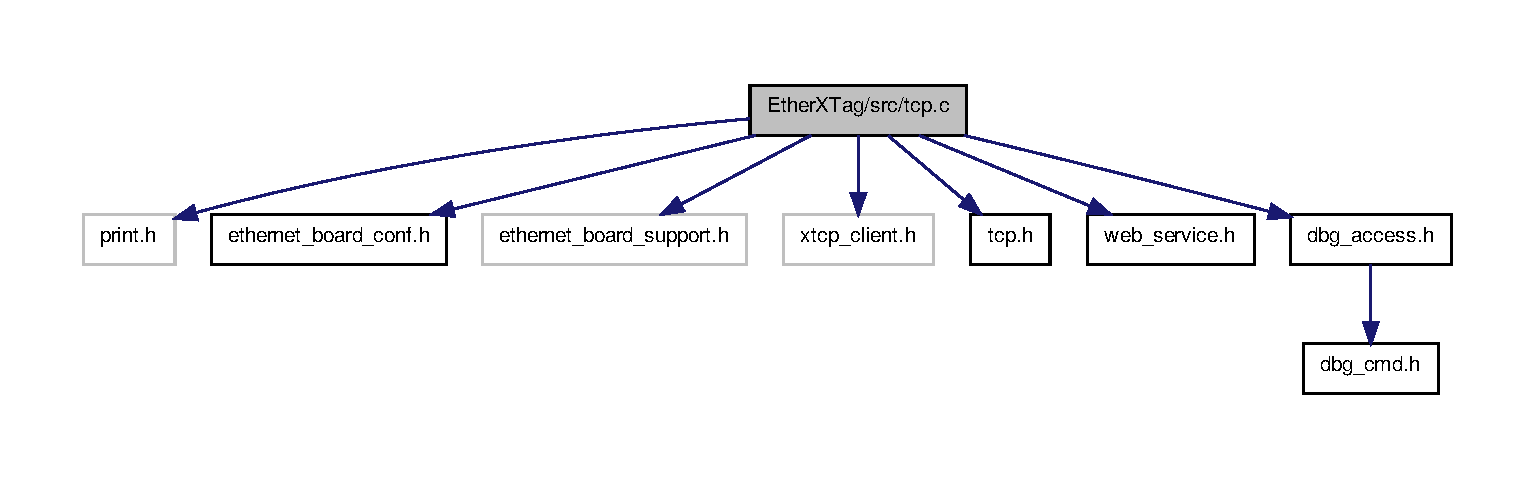
\includegraphics[width=350pt]{tcp_8c__incl}
\end{center}
\end{figure}
\subsection*{Data Structures}
\begin{DoxyCompactItemize}
\item 
struct \hyperlink{structconnection__type__t}{connection\-\_\-type\-\_\-t}
\end{DoxyCompactItemize}
\subsection*{Macros}
\begin{DoxyCompactItemize}
\item 
\#define \hyperlink{tcp_8c_a7180786c98af534f76855fef6f1b97ab}{D\-E\-B\-U\-G\-G\-I\-N\-G}
\item 
\#define \hyperlink{tcp_8c_a32adf79142f0a426b5e782fb7cd4cad3}{D\-B\-G}(x)~x
\end{DoxyCompactItemize}
\subsection*{Typedefs}
\begin{DoxyCompactItemize}
\item 
typedef struct \hyperlink{structconnection__type__t}{connection\-\_\-type\-\_\-t} \hyperlink{tcp_8c_a344b7c4939b85d53795c58f07d8d9fe0}{connection\-\_\-type\-\_\-t}
\end{DoxyCompactItemize}
\subsection*{Functions}
\begin{DoxyCompactItemize}
\item 
void \hyperlink{tcp_8c_a8534a985d36d410a2fd724f725186257}{httpd\-\_\-init} (chanend c\-\_\-xtcp)
\begin{DoxyCompactList}\small\item\em Initialize the H\-T\-T\-P state. \end{DoxyCompactList}\item 
void \hyperlink{tcp_8c_a4c158af3570b43954d6200456d844c9f}{xtag\-\_\-init} (chanend c\-\_\-xtcp)
\begin{DoxyCompactList}\small\item\em Initialise the X\-T\-A\-G state. \end{DoxyCompactList}\item 
void \hyperlink{tcp_8c_a80ca5e099c81a2855b89518a77e3d093}{connection\-\_\-buffer\-\_\-init} ()
\begin{DoxyCompactList}\small\item\em Initialise the connection buffer. \end{DoxyCompactList}\item 
void \hyperlink{tcp_8c_a3cc193cb4914713c69bb20e63e129ec8}{tcp\-\_\-event} (chanend c\-\_\-xtcp, xtcp\-\_\-connection\-\_\-t conn)
\begin{DoxyCompactList}\small\item\em Handles a T\-C\-P event. \end{DoxyCompactList}\item 
void \hyperlink{tcp_8c_aa088fce0f750cc5df371a8ff11fb39cf}{free\-\_\-connection} (xtcp\-\_\-connection\-\_\-t conn)
\begin{DoxyCompactList}\small\item\em Removes a connection from the connections buffer. \end{DoxyCompactList}\item 
void \hyperlink{tcp_8c_a63af330ede3b3cdfedbff2049cf302b5}{accept\-\_\-connection} (chanend c\-\_\-xtcp, xtcp\-\_\-connection\-\_\-t conn)
\begin{DoxyCompactList}\small\item\em If there's room, adds an incoming connection to the connections buffer. \end{DoxyCompactList}\item 
void \hyperlink{tcp_8c_a79c7330ca729a796165f8227decbbd3b}{recv\-\_\-data} (chanend c\-\_\-xtcp, xtcp\-\_\-connection\-\_\-t conn)
\item 
void \hyperlink{tcp_8c_adbb59ad44015a76db47030e6a05d7d9d}{httpd\-\_\-send} (chanend tcp\-\_\-svr, xtcp\-\_\-connection\-\_\-t conn)
\item 
void \hyperlink{tcp_8c_a1f97bdebd1b08139a242b6c0756023d1}{if\-\_\-up} (chanend c\-\_\-xtcp)
\end{DoxyCompactItemize}
\subsection*{Variables}
\begin{DoxyCompactItemize}
\item 
\hyperlink{structconnection__type__t}{connection\-\_\-type\-\_\-t} \hyperlink{tcp_8c_a26456581a73c5cc4b3f48c17add77d5a}{tcp\-\_\-connections} \mbox{[}\hyperlink{tcp_8h_a8e0985f4d6f18b8835ec23373252ef1e}{M\-A\-X\-\_\-\-T\-C\-P\-\_\-\-C\-O\-N\-N\-E\-C\-T\-I\-O\-N\-S}\mbox{]}
\end{DoxyCompactItemize}


\subsection{Macro Definition Documentation}
\hypertarget{tcp_8c_a32adf79142f0a426b5e782fb7cd4cad3}{\index{tcp.\-c@{tcp.\-c}!D\-B\-G@{D\-B\-G}}
\index{D\-B\-G@{D\-B\-G}!tcp.c@{tcp.\-c}}
\subsubsection[{D\-B\-G}]{\setlength{\rightskip}{0pt plus 5cm}\#define D\-B\-G(
\begin{DoxyParamCaption}
\item[{}]{x}
\end{DoxyParamCaption}
)~x}}\label{tcp_8c_a32adf79142f0a426b5e782fb7cd4cad3}


Definition at line 11 of file tcp.\-c.

\hypertarget{tcp_8c_a7180786c98af534f76855fef6f1b97ab}{\index{tcp.\-c@{tcp.\-c}!D\-E\-B\-U\-G\-G\-I\-N\-G@{D\-E\-B\-U\-G\-G\-I\-N\-G}}
\index{D\-E\-B\-U\-G\-G\-I\-N\-G@{D\-E\-B\-U\-G\-G\-I\-N\-G}!tcp.c@{tcp.\-c}}
\subsubsection[{D\-E\-B\-U\-G\-G\-I\-N\-G}]{\setlength{\rightskip}{0pt plus 5cm}\#define D\-E\-B\-U\-G\-G\-I\-N\-G}}\label{tcp_8c_a7180786c98af534f76855fef6f1b97ab}


Definition at line 8 of file tcp.\-c.



\subsection{Typedef Documentation}
\hypertarget{tcp_8c_a344b7c4939b85d53795c58f07d8d9fe0}{\index{tcp.\-c@{tcp.\-c}!connection\-\_\-type\-\_\-t@{connection\-\_\-type\-\_\-t}}
\index{connection\-\_\-type\-\_\-t@{connection\-\_\-type\-\_\-t}!tcp.c@{tcp.\-c}}
\subsubsection[{connection\-\_\-type\-\_\-t}]{\setlength{\rightskip}{0pt plus 5cm}typedef struct {\bf connection\-\_\-type\-\_\-t}  {\bf connection\-\_\-type\-\_\-t}}}\label{tcp_8c_a344b7c4939b85d53795c58f07d8d9fe0}


\subsection{Function Documentation}
\hypertarget{tcp_8c_a63af330ede3b3cdfedbff2049cf302b5}{\index{tcp.\-c@{tcp.\-c}!accept\-\_\-connection@{accept\-\_\-connection}}
\index{accept\-\_\-connection@{accept\-\_\-connection}!tcp.c@{tcp.\-c}}
\subsubsection[{accept\-\_\-connection}]{\setlength{\rightskip}{0pt plus 5cm}void accept\-\_\-connection (
\begin{DoxyParamCaption}
\item[{chanend}]{c\-\_\-xtcp, }
\item[{xtcp\-\_\-connection\-\_\-t}]{conn}
\end{DoxyParamCaption}
)}}\label{tcp_8c_a63af330ede3b3cdfedbff2049cf302b5}


If there's room, adds an incoming connection to the connections buffer. 

This will set-\/up state in the 1st available slot in the connections buffer to represent this connection. 

Definition at line 146 of file tcp.\-c.

\hypertarget{tcp_8c_a80ca5e099c81a2855b89518a77e3d093}{\index{tcp.\-c@{tcp.\-c}!connection\-\_\-buffer\-\_\-init@{connection\-\_\-buffer\-\_\-init}}
\index{connection\-\_\-buffer\-\_\-init@{connection\-\_\-buffer\-\_\-init}!tcp.c@{tcp.\-c}}
\subsubsection[{connection\-\_\-buffer\-\_\-init}]{\setlength{\rightskip}{0pt plus 5cm}void connection\-\_\-buffer\-\_\-init (
\begin{DoxyParamCaption}
{}
\end{DoxyParamCaption}
)}}\label{tcp_8c_a80ca5e099c81a2855b89518a77e3d093}


Initialise the connection buffer. 

Sets all the connections in the buffer to inactive, so they can be used by incoming connections as they are established. 

Definition at line 39 of file tcp.\-c.

\hypertarget{tcp_8c_aa088fce0f750cc5df371a8ff11fb39cf}{\index{tcp.\-c@{tcp.\-c}!free\-\_\-connection@{free\-\_\-connection}}
\index{free\-\_\-connection@{free\-\_\-connection}!tcp.c@{tcp.\-c}}
\subsubsection[{free\-\_\-connection}]{\setlength{\rightskip}{0pt plus 5cm}void free\-\_\-connection (
\begin{DoxyParamCaption}
\item[{xtcp\-\_\-connection\-\_\-t}]{conn}
\end{DoxyParamCaption}
)}}\label{tcp_8c_aa088fce0f750cc5df371a8ff11fb39cf}


Removes a connection from the connections buffer. 

This sets a given connection to inactive, so it may be claimed in {\ttfamily accept\-\_\-connection} 

Definition at line 133 of file tcp.\-c.

\hypertarget{tcp_8c_a8534a985d36d410a2fd724f725186257}{\index{tcp.\-c@{tcp.\-c}!httpd\-\_\-init@{httpd\-\_\-init}}
\index{httpd\-\_\-init@{httpd\-\_\-init}!tcp.c@{tcp.\-c}}
\subsubsection[{httpd\-\_\-init}]{\setlength{\rightskip}{0pt plus 5cm}void httpd\-\_\-init (
\begin{DoxyParamCaption}
\item[{chanend}]{tcp\-\_\-svr}
\end{DoxyParamCaption}
)}}\label{tcp_8c_a8534a985d36d410a2fd724f725186257}


Initialize the H\-T\-T\-P state. 

Adds a tcp listener on the H\-T\-T\-P port (80) 

Definition at line 27 of file tcp.\-c.

\hypertarget{tcp_8c_adbb59ad44015a76db47030e6a05d7d9d}{\index{tcp.\-c@{tcp.\-c}!httpd\-\_\-send@{httpd\-\_\-send}}
\index{httpd\-\_\-send@{httpd\-\_\-send}!tcp.c@{tcp.\-c}}
\subsubsection[{httpd\-\_\-send}]{\setlength{\rightskip}{0pt plus 5cm}void httpd\-\_\-send (
\begin{DoxyParamCaption}
\item[{chanend}]{tcp\-\_\-svr, }
\item[{xtcp\-\_\-connection\-\_\-t}]{conn}
\end{DoxyParamCaption}
)}}\label{tcp_8c_adbb59ad44015a76db47030e6a05d7d9d}
Sends a webpage back down the tcp connection

Sends a webpage generated by web\-\_\-service back down the tcp connection. 

Definition at line 199 of file tcp.\-c.

\hypertarget{tcp_8c_a1f97bdebd1b08139a242b6c0756023d1}{\index{tcp.\-c@{tcp.\-c}!if\-\_\-up@{if\-\_\-up}}
\index{if\-\_\-up@{if\-\_\-up}!tcp.c@{tcp.\-c}}
\subsubsection[{if\-\_\-up}]{\setlength{\rightskip}{0pt plus 5cm}void if\-\_\-up (
\begin{DoxyParamCaption}
\item[{chanend}]{c\-\_\-xtcp}
\end{DoxyParamCaption}
)}}\label{tcp_8c_a1f97bdebd1b08139a242b6c0756023d1}


Definition at line 234 of file tcp.\-c.

\hypertarget{tcp_8c_a79c7330ca729a796165f8227decbbd3b}{\index{tcp.\-c@{tcp.\-c}!recv\-\_\-data@{recv\-\_\-data}}
\index{recv\-\_\-data@{recv\-\_\-data}!tcp.c@{tcp.\-c}}
\subsubsection[{recv\-\_\-data}]{\setlength{\rightskip}{0pt plus 5cm}void recv\-\_\-data (
\begin{DoxyParamCaption}
\item[{chanend}]{c\-\_\-xtcp, }
\item[{xtcp\-\_\-connection\-\_\-t}]{conn}
\end{DoxyParamCaption}
)}}\label{tcp_8c_a79c7330ca729a796165f8227decbbd3b}


Definition at line 160 of file tcp.\-c.

\hypertarget{tcp_8c_a3cc193cb4914713c69bb20e63e129ec8}{\index{tcp.\-c@{tcp.\-c}!tcp\-\_\-event@{tcp\-\_\-event}}
\index{tcp\-\_\-event@{tcp\-\_\-event}!tcp.c@{tcp.\-c}}
\subsubsection[{tcp\-\_\-event}]{\setlength{\rightskip}{0pt plus 5cm}void tcp\-\_\-event (
\begin{DoxyParamCaption}
\item[{chanend}]{c\-\_\-xtcp, }
\item[{xtcp\-\_\-connection\-\_\-t}]{conn}
\end{DoxyParamCaption}
)}}\label{tcp_8c_a3cc193cb4914713c69bb20e63e129ec8}


Handles a T\-C\-P event. 

Switches through various T\-C\-P event scenarios, and handles them apropriately. 

Definition at line 48 of file tcp.\-c.

\hypertarget{tcp_8c_a4c158af3570b43954d6200456d844c9f}{\index{tcp.\-c@{tcp.\-c}!xtag\-\_\-init@{xtag\-\_\-init}}
\index{xtag\-\_\-init@{xtag\-\_\-init}!tcp.c@{tcp.\-c}}
\subsubsection[{xtag\-\_\-init}]{\setlength{\rightskip}{0pt plus 5cm}void xtag\-\_\-init (
\begin{DoxyParamCaption}
\item[{chanend}]{tcp\-\_\-svr}
\end{DoxyParamCaption}
)}}\label{tcp_8c_a4c158af3570b43954d6200456d844c9f}


Initialise the X\-T\-A\-G state. 

Adds a tcp listener to the Ether\-X\-T\-A\-G port (1337) 

Definition at line 33 of file tcp.\-c.



\subsection{Variable Documentation}
\hypertarget{tcp_8c_a26456581a73c5cc4b3f48c17add77d5a}{\index{tcp.\-c@{tcp.\-c}!tcp\-\_\-connections@{tcp\-\_\-connections}}
\index{tcp\-\_\-connections@{tcp\-\_\-connections}!tcp.c@{tcp.\-c}}
\subsubsection[{tcp\-\_\-connections}]{\setlength{\rightskip}{0pt plus 5cm}{\bf connection\-\_\-type\-\_\-t} tcp\-\_\-connections\mbox{[}{\bf M\-A\-X\-\_\-\-T\-C\-P\-\_\-\-C\-O\-N\-N\-E\-C\-T\-I\-O\-N\-S}\mbox{]}}}\label{tcp_8c_a26456581a73c5cc4b3f48c17add77d5a}


Definition at line 25 of file tcp.\-c.


\hypertarget{tcp_8h}{\section{Ether\-X\-Tag/src/tcp.h File Reference}
\label{tcp_8h}\index{Ether\-X\-Tag/src/tcp.\-h@{Ether\-X\-Tag/src/tcp.\-h}}
}
This graph shows which files directly or indirectly include this file\-:\nopagebreak
\begin{figure}[H]
\begin{center}
\leavevmode
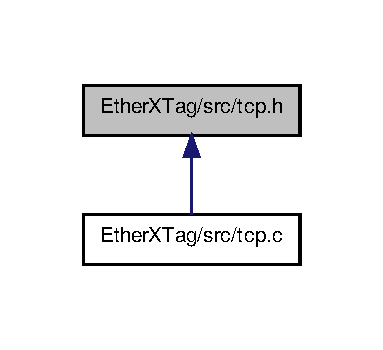
\includegraphics[width=184pt]{tcp_8h__dep__incl}
\end{center}
\end{figure}
\subsection*{Macros}
\begin{DoxyCompactItemize}
\item 
\#define \hyperlink{tcp_8h_a070d2ce7b6bb7e5c05602aa8c308d0c4}{N\-U\-L\-L}~0
\item 
\#define \hyperlink{tcp_8h_a8e0985f4d6f18b8835ec23373252ef1e}{M\-A\-X\-\_\-\-T\-C\-P\-\_\-\-C\-O\-N\-N\-E\-C\-T\-I\-O\-N\-S}~10
\item 
\#define \hyperlink{tcp_8h_af4840cbf3f5fe7fa388e23551a178db6}{E\-T\-H\-E\-R\-\_\-\-X\-T\-A\-G\-\_\-\-P\-O\-R\-T}~1337
\end{DoxyCompactItemize}
\subsection*{Functions}
\begin{DoxyCompactItemize}
\item 
void \hyperlink{tcp_8h_a1e2cf5c7fc76fde6bba0fe97664a7587}{httpd\-\_\-init} (chanend tcp\-\_\-svr)
\begin{DoxyCompactList}\small\item\em Initialize the H\-T\-T\-P state. \end{DoxyCompactList}\item 
void \hyperlink{tcp_8h_af1a2e0ebd1aa97e929b026745233bbcc}{xtag\-\_\-init} (chanend tcp\-\_\-svr)
\begin{DoxyCompactList}\small\item\em Initialise the X\-T\-A\-G state. \end{DoxyCompactList}\item 
void \hyperlink{tcp_8h_a80ca5e099c81a2855b89518a77e3d093}{connection\-\_\-buffer\-\_\-init} ()
\begin{DoxyCompactList}\small\item\em Initialise the connection buffer. \end{DoxyCompactList}\item 
void \hyperlink{tcp_8h_adbb59ad44015a76db47030e6a05d7d9d}{httpd\-\_\-send} (chanend tcp\-\_\-svr, xtcp\-\_\-connection\-\_\-t conn)
\item 
void \hyperlink{tcp_8h_a63af330ede3b3cdfedbff2049cf302b5}{accept\-\_\-connection} (chanend c\-\_\-xtcp, xtcp\-\_\-connection\-\_\-t conn)
\begin{DoxyCompactList}\small\item\em If there's room, adds an incoming connection to the connections buffer. \end{DoxyCompactList}\item 
void \hyperlink{tcp_8h_aa088fce0f750cc5df371a8ff11fb39cf}{free\-\_\-connection} (xtcp\-\_\-connection\-\_\-t conn)
\begin{DoxyCompactList}\small\item\em Removes a connection from the connections buffer. \end{DoxyCompactList}\item 
void \hyperlink{tcp_8h_a3cc193cb4914713c69bb20e63e129ec8}{tcp\-\_\-event} (chanend c\-\_\-xtcp, xtcp\-\_\-connection\-\_\-t conn)
\begin{DoxyCompactList}\small\item\em Handles a T\-C\-P event. \end{DoxyCompactList}\item 
void \hyperlink{tcp_8h_a79c7330ca729a796165f8227decbbd3b}{recv\-\_\-data} (chanend c\-\_\-xtcp, xtcp\-\_\-connection\-\_\-t conn)
\item 
void \hyperlink{tcp_8h_a1f97bdebd1b08139a242b6c0756023d1}{if\-\_\-up} (chanend c\-\_\-xtcp)
\end{DoxyCompactItemize}


\subsection{Macro Definition Documentation}
\hypertarget{tcp_8h_af4840cbf3f5fe7fa388e23551a178db6}{\index{tcp.\-h@{tcp.\-h}!E\-T\-H\-E\-R\-\_\-\-X\-T\-A\-G\-\_\-\-P\-O\-R\-T@{E\-T\-H\-E\-R\-\_\-\-X\-T\-A\-G\-\_\-\-P\-O\-R\-T}}
\index{E\-T\-H\-E\-R\-\_\-\-X\-T\-A\-G\-\_\-\-P\-O\-R\-T@{E\-T\-H\-E\-R\-\_\-\-X\-T\-A\-G\-\_\-\-P\-O\-R\-T}!tcp.h@{tcp.\-h}}
\subsubsection[{E\-T\-H\-E\-R\-\_\-\-X\-T\-A\-G\-\_\-\-P\-O\-R\-T}]{\setlength{\rightskip}{0pt plus 5cm}\#define E\-T\-H\-E\-R\-\_\-\-X\-T\-A\-G\-\_\-\-P\-O\-R\-T~1337}}\label{tcp_8h_af4840cbf3f5fe7fa388e23551a178db6}


Definition at line 9 of file tcp.\-h.

\hypertarget{tcp_8h_a8e0985f4d6f18b8835ec23373252ef1e}{\index{tcp.\-h@{tcp.\-h}!M\-A\-X\-\_\-\-T\-C\-P\-\_\-\-C\-O\-N\-N\-E\-C\-T\-I\-O\-N\-S@{M\-A\-X\-\_\-\-T\-C\-P\-\_\-\-C\-O\-N\-N\-E\-C\-T\-I\-O\-N\-S}}
\index{M\-A\-X\-\_\-\-T\-C\-P\-\_\-\-C\-O\-N\-N\-E\-C\-T\-I\-O\-N\-S@{M\-A\-X\-\_\-\-T\-C\-P\-\_\-\-C\-O\-N\-N\-E\-C\-T\-I\-O\-N\-S}!tcp.h@{tcp.\-h}}
\subsubsection[{M\-A\-X\-\_\-\-T\-C\-P\-\_\-\-C\-O\-N\-N\-E\-C\-T\-I\-O\-N\-S}]{\setlength{\rightskip}{0pt plus 5cm}\#define M\-A\-X\-\_\-\-T\-C\-P\-\_\-\-C\-O\-N\-N\-E\-C\-T\-I\-O\-N\-S~10}}\label{tcp_8h_a8e0985f4d6f18b8835ec23373252ef1e}


Definition at line 8 of file tcp.\-h.

\hypertarget{tcp_8h_a070d2ce7b6bb7e5c05602aa8c308d0c4}{\index{tcp.\-h@{tcp.\-h}!N\-U\-L\-L@{N\-U\-L\-L}}
\index{N\-U\-L\-L@{N\-U\-L\-L}!tcp.h@{tcp.\-h}}
\subsubsection[{N\-U\-L\-L}]{\setlength{\rightskip}{0pt plus 5cm}\#define N\-U\-L\-L~0}}\label{tcp_8h_a070d2ce7b6bb7e5c05602aa8c308d0c4}


Definition at line 5 of file tcp.\-h.



\subsection{Function Documentation}
\hypertarget{tcp_8h_a63af330ede3b3cdfedbff2049cf302b5}{\index{tcp.\-h@{tcp.\-h}!accept\-\_\-connection@{accept\-\_\-connection}}
\index{accept\-\_\-connection@{accept\-\_\-connection}!tcp.h@{tcp.\-h}}
\subsubsection[{accept\-\_\-connection}]{\setlength{\rightskip}{0pt plus 5cm}void accept\-\_\-connection (
\begin{DoxyParamCaption}
\item[{chanend}]{c\-\_\-xtcp, }
\item[{xtcp\-\_\-connection\-\_\-t}]{conn}
\end{DoxyParamCaption}
)}}\label{tcp_8h_a63af330ede3b3cdfedbff2049cf302b5}


If there's room, adds an incoming connection to the connections buffer. 

This will set-\/up state in the 1st available slot in the connections buffer to represent this connection. 

Definition at line 146 of file tcp.\-c.

\hypertarget{tcp_8h_a80ca5e099c81a2855b89518a77e3d093}{\index{tcp.\-h@{tcp.\-h}!connection\-\_\-buffer\-\_\-init@{connection\-\_\-buffer\-\_\-init}}
\index{connection\-\_\-buffer\-\_\-init@{connection\-\_\-buffer\-\_\-init}!tcp.h@{tcp.\-h}}
\subsubsection[{connection\-\_\-buffer\-\_\-init}]{\setlength{\rightskip}{0pt plus 5cm}void connection\-\_\-buffer\-\_\-init (
\begin{DoxyParamCaption}
{}
\end{DoxyParamCaption}
)}}\label{tcp_8h_a80ca5e099c81a2855b89518a77e3d093}


Initialise the connection buffer. 

Sets all the connections in the buffer to inactive, so they can be used by incoming connections as they are established. 

Definition at line 39 of file tcp.\-c.

\hypertarget{tcp_8h_aa088fce0f750cc5df371a8ff11fb39cf}{\index{tcp.\-h@{tcp.\-h}!free\-\_\-connection@{free\-\_\-connection}}
\index{free\-\_\-connection@{free\-\_\-connection}!tcp.h@{tcp.\-h}}
\subsubsection[{free\-\_\-connection}]{\setlength{\rightskip}{0pt plus 5cm}void free\-\_\-connection (
\begin{DoxyParamCaption}
\item[{xtcp\-\_\-connection\-\_\-t}]{conn}
\end{DoxyParamCaption}
)}}\label{tcp_8h_aa088fce0f750cc5df371a8ff11fb39cf}


Removes a connection from the connections buffer. 

This sets a given connection to inactive, so it may be claimed in {\ttfamily accept\-\_\-connection} 

Definition at line 133 of file tcp.\-c.

\hypertarget{tcp_8h_a1e2cf5c7fc76fde6bba0fe97664a7587}{\index{tcp.\-h@{tcp.\-h}!httpd\-\_\-init@{httpd\-\_\-init}}
\index{httpd\-\_\-init@{httpd\-\_\-init}!tcp.h@{tcp.\-h}}
\subsubsection[{httpd\-\_\-init}]{\setlength{\rightskip}{0pt plus 5cm}void httpd\-\_\-init (
\begin{DoxyParamCaption}
\item[{chanend}]{tcp\-\_\-svr}
\end{DoxyParamCaption}
)}}\label{tcp_8h_a1e2cf5c7fc76fde6bba0fe97664a7587}


Initialize the H\-T\-T\-P state. 

Adds a tcp listener on the H\-T\-T\-P port (80) 

Definition at line 27 of file tcp.\-c.

\hypertarget{tcp_8h_adbb59ad44015a76db47030e6a05d7d9d}{\index{tcp.\-h@{tcp.\-h}!httpd\-\_\-send@{httpd\-\_\-send}}
\index{httpd\-\_\-send@{httpd\-\_\-send}!tcp.h@{tcp.\-h}}
\subsubsection[{httpd\-\_\-send}]{\setlength{\rightskip}{0pt plus 5cm}void httpd\-\_\-send (
\begin{DoxyParamCaption}
\item[{chanend}]{tcp\-\_\-svr, }
\item[{xtcp\-\_\-connection\-\_\-t}]{conn}
\end{DoxyParamCaption}
)}}\label{tcp_8h_adbb59ad44015a76db47030e6a05d7d9d}
Sends a webpage back down the tcp connection

Sends a webpage generated by web\-\_\-service back down the tcp connection. 

Definition at line 199 of file tcp.\-c.

\hypertarget{tcp_8h_a1f97bdebd1b08139a242b6c0756023d1}{\index{tcp.\-h@{tcp.\-h}!if\-\_\-up@{if\-\_\-up}}
\index{if\-\_\-up@{if\-\_\-up}!tcp.h@{tcp.\-h}}
\subsubsection[{if\-\_\-up}]{\setlength{\rightskip}{0pt plus 5cm}void if\-\_\-up (
\begin{DoxyParamCaption}
\item[{chanend}]{c\-\_\-xtcp}
\end{DoxyParamCaption}
)}}\label{tcp_8h_a1f97bdebd1b08139a242b6c0756023d1}


Definition at line 234 of file tcp.\-c.

\hypertarget{tcp_8h_a79c7330ca729a796165f8227decbbd3b}{\index{tcp.\-h@{tcp.\-h}!recv\-\_\-data@{recv\-\_\-data}}
\index{recv\-\_\-data@{recv\-\_\-data}!tcp.h@{tcp.\-h}}
\subsubsection[{recv\-\_\-data}]{\setlength{\rightskip}{0pt plus 5cm}void recv\-\_\-data (
\begin{DoxyParamCaption}
\item[{chanend}]{c\-\_\-xtcp, }
\item[{xtcp\-\_\-connection\-\_\-t}]{conn}
\end{DoxyParamCaption}
)}}\label{tcp_8h_a79c7330ca729a796165f8227decbbd3b}


Definition at line 160 of file tcp.\-c.

\hypertarget{tcp_8h_a3cc193cb4914713c69bb20e63e129ec8}{\index{tcp.\-h@{tcp.\-h}!tcp\-\_\-event@{tcp\-\_\-event}}
\index{tcp\-\_\-event@{tcp\-\_\-event}!tcp.h@{tcp.\-h}}
\subsubsection[{tcp\-\_\-event}]{\setlength{\rightskip}{0pt plus 5cm}void tcp\-\_\-event (
\begin{DoxyParamCaption}
\item[{chanend}]{c\-\_\-xtcp, }
\item[{xtcp\-\_\-connection\-\_\-t}]{conn}
\end{DoxyParamCaption}
)}}\label{tcp_8h_a3cc193cb4914713c69bb20e63e129ec8}


Handles a T\-C\-P event. 

Switches through various T\-C\-P event scenarios, and handles them apropriately. 

Definition at line 48 of file tcp.\-c.

\hypertarget{tcp_8h_af1a2e0ebd1aa97e929b026745233bbcc}{\index{tcp.\-h@{tcp.\-h}!xtag\-\_\-init@{xtag\-\_\-init}}
\index{xtag\-\_\-init@{xtag\-\_\-init}!tcp.h@{tcp.\-h}}
\subsubsection[{xtag\-\_\-init}]{\setlength{\rightskip}{0pt plus 5cm}void xtag\-\_\-init (
\begin{DoxyParamCaption}
\item[{chanend}]{tcp\-\_\-svr}
\end{DoxyParamCaption}
)}}\label{tcp_8h_af1a2e0ebd1aa97e929b026745233bbcc}


Initialise the X\-T\-A\-G state. 

Adds a tcp listener to the Ether\-X\-T\-A\-G port (1337) 

Definition at line 33 of file tcp.\-c.


\hypertarget{udp_8c}{\section{Ether\-X\-Tag/src/udp.c File Reference}
\label{udp_8c}\index{Ether\-X\-Tag/src/udp.\-c@{Ether\-X\-Tag/src/udp.\-c}}
}
{\ttfamily \#include $<$stdio.\-h$>$}\\*
{\ttfamily \#include $<$string.\-h$>$}\\*
{\ttfamily \#include $<$print.\-h$>$}\\*
{\ttfamily \#include \char`\"{}xtcp\-\_\-client.\-h\char`\"{}}\\*
{\ttfamily \#include \char`\"{}udp.\-h\char`\"{}}\\*
{\ttfamily \#include \char`\"{}mdns.\-h\char`\"{}}\\*
Include dependency graph for udp.\-c\-:\nopagebreak
\begin{figure}[H]
\begin{center}
\leavevmode
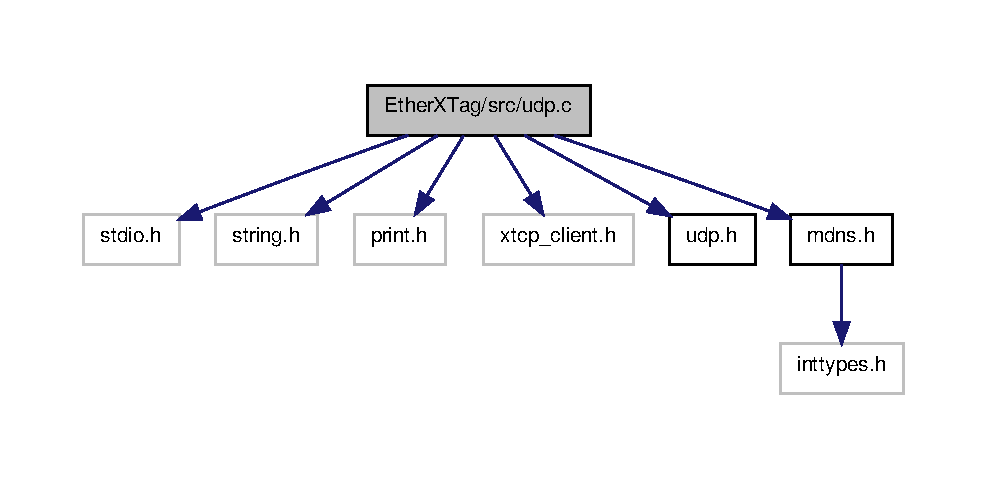
\includegraphics[width=350pt]{udp_8c__incl}
\end{center}
\end{figure}
\subsection*{Data Structures}
\begin{DoxyCompactItemize}
\item 
struct \hyperlink{structconnection__type__t}{connection\-\_\-type\-\_\-t}
\end{DoxyCompactItemize}
\subsection*{Macros}
\begin{DoxyCompactItemize}
\item 
\#define \hyperlink{udp_8c_a7180786c98af534f76855fef6f1b97ab}{D\-E\-B\-U\-G\-G\-I\-N\-G}
\item 
\#define \hyperlink{udp_8c_a32adf79142f0a426b5e782fb7cd4cad3}{D\-B\-G}(x)~x
\end{DoxyCompactItemize}
\subsection*{Typedefs}
\begin{DoxyCompactItemize}
\item 
typedef struct \hyperlink{structconnection__type__t}{connection\-\_\-type\-\_\-t} \hyperlink{udp_8c_a344b7c4939b85d53795c58f07d8d9fe0}{connection\-\_\-type\-\_\-t}
\end{DoxyCompactItemize}
\subsection*{Functions}
\begin{DoxyCompactItemize}
\item 
void \hyperlink{udp_8c_ad289e78e3f586bb23a638af432bb734e}{mdns\-\_\-init} (chanend c\-\_\-xtcp)
\item 
void \hyperlink{udp_8c_a3e9cf2f5d9f21d897d17a36b76695ff2}{accept\-\_\-connection\-\_\-udp} (chanend c\-\_\-xtcp, xtcp\-\_\-connection\-\_\-t conn)
\item 
void \hyperlink{udp_8c_a07d21a9c74237ef7521a55545adc4093}{free\-\_\-connection\-\_\-udp} (xtcp\-\_\-connection\-\_\-t conn)
\item 
void \hyperlink{udp_8c_a350d7a8bdb9cafaea8966ce878374fbf}{udp\-\_\-recv\-\_\-data} (chanend c\-\_\-xtcp, xtcp\-\_\-connection\-\_\-t conn)
\item 
void \hyperlink{udp_8c_a67727f2eb992e609e1c2782261af78b1}{udp\-\_\-event} (chanend c\-\_\-xtcp, xtcp\-\_\-connection\-\_\-t conn)
\end{DoxyCompactItemize}
\subsection*{Variables}
\begin{DoxyCompactItemize}
\item 
\hyperlink{structconnection__type__t}{connection\-\_\-type\-\_\-t} \hyperlink{udp_8c_a5f4e7e9355081f3b85af06e4ed426635}{udp\-\_\-connections} \mbox{[}\hyperlink{udp_8h_a72d1def3b8b33feb906fc320c8c1a653}{M\-A\-X\-\_\-\-U\-D\-P\-\_\-\-C\-O\-N\-N\-E\-C\-T\-I\-O\-N\-S}\mbox{]}
\end{DoxyCompactItemize}


\subsection{Macro Definition Documentation}
\hypertarget{udp_8c_a32adf79142f0a426b5e782fb7cd4cad3}{\index{udp.\-c@{udp.\-c}!D\-B\-G@{D\-B\-G}}
\index{D\-B\-G@{D\-B\-G}!udp.c@{udp.\-c}}
\subsubsection[{D\-B\-G}]{\setlength{\rightskip}{0pt plus 5cm}\#define D\-B\-G(
\begin{DoxyParamCaption}
\item[{}]{x}
\end{DoxyParamCaption}
)~x}}\label{udp_8c_a32adf79142f0a426b5e782fb7cd4cad3}


Definition at line 12 of file udp.\-c.

\hypertarget{udp_8c_a7180786c98af534f76855fef6f1b97ab}{\index{udp.\-c@{udp.\-c}!D\-E\-B\-U\-G\-G\-I\-N\-G@{D\-E\-B\-U\-G\-G\-I\-N\-G}}
\index{D\-E\-B\-U\-G\-G\-I\-N\-G@{D\-E\-B\-U\-G\-G\-I\-N\-G}!udp.c@{udp.\-c}}
\subsubsection[{D\-E\-B\-U\-G\-G\-I\-N\-G}]{\setlength{\rightskip}{0pt plus 5cm}\#define D\-E\-B\-U\-G\-G\-I\-N\-G}}\label{udp_8c_a7180786c98af534f76855fef6f1b97ab}


Definition at line 9 of file udp.\-c.



\subsection{Typedef Documentation}
\hypertarget{udp_8c_a344b7c4939b85d53795c58f07d8d9fe0}{\index{udp.\-c@{udp.\-c}!connection\-\_\-type\-\_\-t@{connection\-\_\-type\-\_\-t}}
\index{connection\-\_\-type\-\_\-t@{connection\-\_\-type\-\_\-t}!udp.c@{udp.\-c}}
\subsubsection[{connection\-\_\-type\-\_\-t}]{\setlength{\rightskip}{0pt plus 5cm}typedef struct {\bf connection\-\_\-type\-\_\-t}  {\bf connection\-\_\-type\-\_\-t}}}\label{udp_8c_a344b7c4939b85d53795c58f07d8d9fe0}


\subsection{Function Documentation}
\hypertarget{udp_8c_a3e9cf2f5d9f21d897d17a36b76695ff2}{\index{udp.\-c@{udp.\-c}!accept\-\_\-connection\-\_\-udp@{accept\-\_\-connection\-\_\-udp}}
\index{accept\-\_\-connection\-\_\-udp@{accept\-\_\-connection\-\_\-udp}!udp.c@{udp.\-c}}
\subsubsection[{accept\-\_\-connection\-\_\-udp}]{\setlength{\rightskip}{0pt plus 5cm}void accept\-\_\-connection\-\_\-udp (
\begin{DoxyParamCaption}
\item[{chanend}]{c\-\_\-xtcp, }
\item[{xtcp\-\_\-connection\-\_\-t}]{conn}
\end{DoxyParamCaption}
)}}\label{udp_8c_a3e9cf2f5d9f21d897d17a36b76695ff2}


Definition at line 34 of file udp.\-c.

\hypertarget{udp_8c_a07d21a9c74237ef7521a55545adc4093}{\index{udp.\-c@{udp.\-c}!free\-\_\-connection\-\_\-udp@{free\-\_\-connection\-\_\-udp}}
\index{free\-\_\-connection\-\_\-udp@{free\-\_\-connection\-\_\-udp}!udp.c@{udp.\-c}}
\subsubsection[{free\-\_\-connection\-\_\-udp}]{\setlength{\rightskip}{0pt plus 5cm}void free\-\_\-connection\-\_\-udp (
\begin{DoxyParamCaption}
\item[{xtcp\-\_\-connection\-\_\-t}]{conn}
\end{DoxyParamCaption}
)}}\label{udp_8c_a07d21a9c74237ef7521a55545adc4093}


Definition at line 48 of file udp.\-c.

\hypertarget{udp_8c_ad289e78e3f586bb23a638af432bb734e}{\index{udp.\-c@{udp.\-c}!mdns\-\_\-init@{mdns\-\_\-init}}
\index{mdns\-\_\-init@{mdns\-\_\-init}!udp.c@{udp.\-c}}
\subsubsection[{mdns\-\_\-init}]{\setlength{\rightskip}{0pt plus 5cm}void mdns\-\_\-init (
\begin{DoxyParamCaption}
\item[{chanend}]{c\-\_\-xtcp}
\end{DoxyParamCaption}
)}}\label{udp_8c_ad289e78e3f586bb23a638af432bb734e}


Definition at line 29 of file udp.\-c.

\hypertarget{udp_8c_a67727f2eb992e609e1c2782261af78b1}{\index{udp.\-c@{udp.\-c}!udp\-\_\-event@{udp\-\_\-event}}
\index{udp\-\_\-event@{udp\-\_\-event}!udp.c@{udp.\-c}}
\subsubsection[{udp\-\_\-event}]{\setlength{\rightskip}{0pt plus 5cm}void udp\-\_\-event (
\begin{DoxyParamCaption}
\item[{chanend}]{c\-\_\-xtcp, }
\item[{xtcp\-\_\-connection\-\_\-t}]{conn}
\end{DoxyParamCaption}
)}}\label{udp_8c_a67727f2eb992e609e1c2782261af78b1}


Definition at line 88 of file udp.\-c.

\hypertarget{udp_8c_a350d7a8bdb9cafaea8966ce878374fbf}{\index{udp.\-c@{udp.\-c}!udp\-\_\-recv\-\_\-data@{udp\-\_\-recv\-\_\-data}}
\index{udp\-\_\-recv\-\_\-data@{udp\-\_\-recv\-\_\-data}!udp.c@{udp.\-c}}
\subsubsection[{udp\-\_\-recv\-\_\-data}]{\setlength{\rightskip}{0pt plus 5cm}void udp\-\_\-recv\-\_\-data (
\begin{DoxyParamCaption}
\item[{chanend}]{c\-\_\-xtcp, }
\item[{xtcp\-\_\-connection\-\_\-t}]{conn}
\end{DoxyParamCaption}
)}}\label{udp_8c_a350d7a8bdb9cafaea8966ce878374fbf}


Definition at line 56 of file udp.\-c.



\subsection{Variable Documentation}
\hypertarget{udp_8c_a5f4e7e9355081f3b85af06e4ed426635}{\index{udp.\-c@{udp.\-c}!udp\-\_\-connections@{udp\-\_\-connections}}
\index{udp\-\_\-connections@{udp\-\_\-connections}!udp.c@{udp.\-c}}
\subsubsection[{udp\-\_\-connections}]{\setlength{\rightskip}{0pt plus 5cm}{\bf connection\-\_\-type\-\_\-t} udp\-\_\-connections\mbox{[}{\bf M\-A\-X\-\_\-\-U\-D\-P\-\_\-\-C\-O\-N\-N\-E\-C\-T\-I\-O\-N\-S}\mbox{]}}}\label{udp_8c_a5f4e7e9355081f3b85af06e4ed426635}


Definition at line 27 of file udp.\-c.


\hypertarget{udp_8h}{\section{Ether\-X\-Tag/src/udp.h File Reference}
\label{udp_8h}\index{Ether\-X\-Tag/src/udp.\-h@{Ether\-X\-Tag/src/udp.\-h}}
}
This graph shows which files directly or indirectly include this file\-:\nopagebreak
\begin{figure}[H]
\begin{center}
\leavevmode
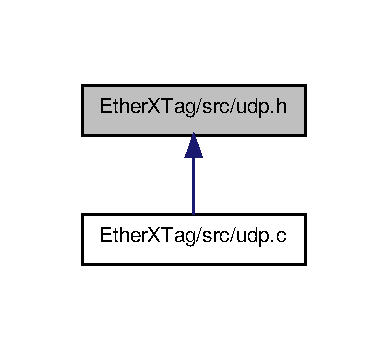
\includegraphics[width=186pt]{udp_8h__dep__incl}
\end{center}
\end{figure}
\subsection*{Macros}
\begin{DoxyCompactItemize}
\item 
\#define \hyperlink{udp_8h_ab16900c77e60e00f401b684c45a37c34}{M\-D\-N\-S\-\_\-\-P\-O\-R\-T}~5353
\item 
\#define \hyperlink{udp_8h_a72d1def3b8b33feb906fc320c8c1a653}{M\-A\-X\-\_\-\-U\-D\-P\-\_\-\-C\-O\-N\-N\-E\-C\-T\-I\-O\-N\-S}~20
\end{DoxyCompactItemize}
\subsection*{Functions}
\begin{DoxyCompactItemize}
\item 
void \hyperlink{udp_8h_ad289e78e3f586bb23a638af432bb734e}{mdns\-\_\-init} (chanend c\-\_\-xtcp)
\item 
void \hyperlink{udp_8h_a3e9cf2f5d9f21d897d17a36b76695ff2}{accept\-\_\-connection\-\_\-udp} (chanend c\-\_\-xtcp, xtcp\-\_\-connection\-\_\-t conn)
\item 
void \hyperlink{udp_8h_a07d21a9c74237ef7521a55545adc4093}{free\-\_\-connection\-\_\-udp} (xtcp\-\_\-connection\-\_\-t conn)
\item 
void \hyperlink{udp_8h_a67727f2eb992e609e1c2782261af78b1}{udp\-\_\-event} (chanend c\-\_\-xtcp, xtcp\-\_\-connection\-\_\-t conn)
\end{DoxyCompactItemize}


\subsection{Macro Definition Documentation}
\hypertarget{udp_8h_a72d1def3b8b33feb906fc320c8c1a653}{\index{udp.\-h@{udp.\-h}!M\-A\-X\-\_\-\-U\-D\-P\-\_\-\-C\-O\-N\-N\-E\-C\-T\-I\-O\-N\-S@{M\-A\-X\-\_\-\-U\-D\-P\-\_\-\-C\-O\-N\-N\-E\-C\-T\-I\-O\-N\-S}}
\index{M\-A\-X\-\_\-\-U\-D\-P\-\_\-\-C\-O\-N\-N\-E\-C\-T\-I\-O\-N\-S@{M\-A\-X\-\_\-\-U\-D\-P\-\_\-\-C\-O\-N\-N\-E\-C\-T\-I\-O\-N\-S}!udp.h@{udp.\-h}}
\subsubsection[{M\-A\-X\-\_\-\-U\-D\-P\-\_\-\-C\-O\-N\-N\-E\-C\-T\-I\-O\-N\-S}]{\setlength{\rightskip}{0pt plus 5cm}\#define M\-A\-X\-\_\-\-U\-D\-P\-\_\-\-C\-O\-N\-N\-E\-C\-T\-I\-O\-N\-S~20}}\label{udp_8h_a72d1def3b8b33feb906fc320c8c1a653}


Definition at line 5 of file udp.\-h.

\hypertarget{udp_8h_ab16900c77e60e00f401b684c45a37c34}{\index{udp.\-h@{udp.\-h}!M\-D\-N\-S\-\_\-\-P\-O\-R\-T@{M\-D\-N\-S\-\_\-\-P\-O\-R\-T}}
\index{M\-D\-N\-S\-\_\-\-P\-O\-R\-T@{M\-D\-N\-S\-\_\-\-P\-O\-R\-T}!udp.h@{udp.\-h}}
\subsubsection[{M\-D\-N\-S\-\_\-\-P\-O\-R\-T}]{\setlength{\rightskip}{0pt plus 5cm}\#define M\-D\-N\-S\-\_\-\-P\-O\-R\-T~5353}}\label{udp_8h_ab16900c77e60e00f401b684c45a37c34}


Definition at line 4 of file udp.\-h.



\subsection{Function Documentation}
\hypertarget{udp_8h_a3e9cf2f5d9f21d897d17a36b76695ff2}{\index{udp.\-h@{udp.\-h}!accept\-\_\-connection\-\_\-udp@{accept\-\_\-connection\-\_\-udp}}
\index{accept\-\_\-connection\-\_\-udp@{accept\-\_\-connection\-\_\-udp}!udp.h@{udp.\-h}}
\subsubsection[{accept\-\_\-connection\-\_\-udp}]{\setlength{\rightskip}{0pt plus 5cm}void accept\-\_\-connection\-\_\-udp (
\begin{DoxyParamCaption}
\item[{chanend}]{c\-\_\-xtcp, }
\item[{xtcp\-\_\-connection\-\_\-t}]{conn}
\end{DoxyParamCaption}
)}}\label{udp_8h_a3e9cf2f5d9f21d897d17a36b76695ff2}


Definition at line 34 of file udp.\-c.

\hypertarget{udp_8h_a07d21a9c74237ef7521a55545adc4093}{\index{udp.\-h@{udp.\-h}!free\-\_\-connection\-\_\-udp@{free\-\_\-connection\-\_\-udp}}
\index{free\-\_\-connection\-\_\-udp@{free\-\_\-connection\-\_\-udp}!udp.h@{udp.\-h}}
\subsubsection[{free\-\_\-connection\-\_\-udp}]{\setlength{\rightskip}{0pt plus 5cm}void free\-\_\-connection\-\_\-udp (
\begin{DoxyParamCaption}
\item[{xtcp\-\_\-connection\-\_\-t}]{conn}
\end{DoxyParamCaption}
)}}\label{udp_8h_a07d21a9c74237ef7521a55545adc4093}


Definition at line 48 of file udp.\-c.

\hypertarget{udp_8h_ad289e78e3f586bb23a638af432bb734e}{\index{udp.\-h@{udp.\-h}!mdns\-\_\-init@{mdns\-\_\-init}}
\index{mdns\-\_\-init@{mdns\-\_\-init}!udp.h@{udp.\-h}}
\subsubsection[{mdns\-\_\-init}]{\setlength{\rightskip}{0pt plus 5cm}void mdns\-\_\-init (
\begin{DoxyParamCaption}
\item[{chanend}]{c\-\_\-xtcp}
\end{DoxyParamCaption}
)}}\label{udp_8h_ad289e78e3f586bb23a638af432bb734e}


Definition at line 29 of file udp.\-c.

\hypertarget{udp_8h_a67727f2eb992e609e1c2782261af78b1}{\index{udp.\-h@{udp.\-h}!udp\-\_\-event@{udp\-\_\-event}}
\index{udp\-\_\-event@{udp\-\_\-event}!udp.h@{udp.\-h}}
\subsubsection[{udp\-\_\-event}]{\setlength{\rightskip}{0pt plus 5cm}void udp\-\_\-event (
\begin{DoxyParamCaption}
\item[{chanend}]{c\-\_\-xtcp, }
\item[{xtcp\-\_\-connection\-\_\-t}]{conn}
\end{DoxyParamCaption}
)}}\label{udp_8h_a67727f2eb992e609e1c2782261af78b1}


Definition at line 88 of file udp.\-c.


\hypertarget{web__service_8c}{\section{Ether\-X\-Tag/src/web\-\_\-service.c File Reference}
\label{web__service_8c}\index{Ether\-X\-Tag/src/web\-\_\-service.\-c@{Ether\-X\-Tag/src/web\-\_\-service.\-c}}
}
{\ttfamily \#include $<$string.\-h$>$}\\*
{\ttfamily \#include \char`\"{}web\-\_\-service.\-h\char`\"{}}\\*
Include dependency graph for web\-\_\-service.\-c\-:\nopagebreak
\begin{figure}[H]
\begin{center}
\leavevmode
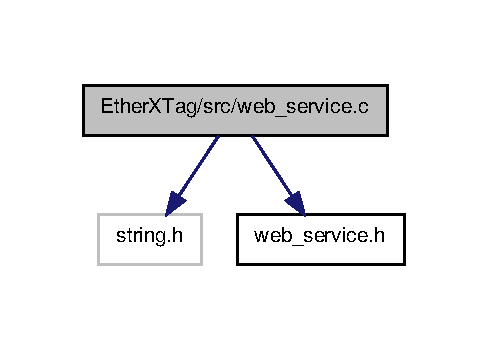
\includegraphics[width=234pt]{web__service_8c__incl}
\end{center}
\end{figure}
\subsection*{Functions}
\begin{DoxyCompactItemize}
\item 
\hyperlink{structpage__t}{page\-\_\-t} $\ast$ \hyperlink{web__service_8c_a5a94d9ecf7963c0150225d8acb17f6ea}{get\-Page} ()
\item 
const char $\ast$ \hyperlink{web__service_8c_a57eb4e125f533b812f7153767d315d1e}{get\-H\-T\-T\-P\-Header} ()
\item 
const char $\ast$ \hyperlink{web__service_8c_aba6e8228ddb103ef147d1108503f46e2}{get\-Page\-Content} ()
\end{DoxyCompactItemize}
\subsection*{Variables}
\begin{DoxyCompactItemize}
\item 
\hyperlink{structpage__t}{page\-\_\-t} \hyperlink{web__service_8c_a235055e1933d2f949eb5989f7a15c35c}{ret\-Val} = \{ 0, \char`\"{}\char`\"{} \}
\end{DoxyCompactItemize}


\subsection{Function Documentation}
\hypertarget{web__service_8c_a57eb4e125f533b812f7153767d315d1e}{\index{web\-\_\-service.\-c@{web\-\_\-service.\-c}!get\-H\-T\-T\-P\-Header@{get\-H\-T\-T\-P\-Header}}
\index{get\-H\-T\-T\-P\-Header@{get\-H\-T\-T\-P\-Header}!web_service.c@{web\-\_\-service.\-c}}
\subsubsection[{get\-H\-T\-T\-P\-Header}]{\setlength{\rightskip}{0pt plus 5cm}const char$\ast$ get\-H\-T\-T\-P\-Header (
\begin{DoxyParamCaption}
{}
\end{DoxyParamCaption}
)}}\label{web__service_8c_a57eb4e125f533b812f7153767d315d1e}


Definition at line 23 of file web\-\_\-service.\-c.

\hypertarget{web__service_8c_a5a94d9ecf7963c0150225d8acb17f6ea}{\index{web\-\_\-service.\-c@{web\-\_\-service.\-c}!get\-Page@{get\-Page}}
\index{get\-Page@{get\-Page}!web_service.c@{web\-\_\-service.\-c}}
\subsubsection[{get\-Page}]{\setlength{\rightskip}{0pt plus 5cm}{\bf page\-\_\-t}$\ast$ get\-Page (
\begin{DoxyParamCaption}
{}
\end{DoxyParamCaption}
)}}\label{web__service_8c_a5a94d9ecf7963c0150225d8acb17f6ea}


Definition at line 6 of file web\-\_\-service.\-c.

\hypertarget{web__service_8c_aba6e8228ddb103ef147d1108503f46e2}{\index{web\-\_\-service.\-c@{web\-\_\-service.\-c}!get\-Page\-Content@{get\-Page\-Content}}
\index{get\-Page\-Content@{get\-Page\-Content}!web_service.c@{web\-\_\-service.\-c}}
\subsubsection[{get\-Page\-Content}]{\setlength{\rightskip}{0pt plus 5cm}const char$\ast$ get\-Page\-Content (
\begin{DoxyParamCaption}
{}
\end{DoxyParamCaption}
)}}\label{web__service_8c_aba6e8228ddb103ef147d1108503f46e2}


Definition at line 27 of file web\-\_\-service.\-c.



\subsection{Variable Documentation}
\hypertarget{web__service_8c_a235055e1933d2f949eb5989f7a15c35c}{\index{web\-\_\-service.\-c@{web\-\_\-service.\-c}!ret\-Val@{ret\-Val}}
\index{ret\-Val@{ret\-Val}!web_service.c@{web\-\_\-service.\-c}}
\subsubsection[{ret\-Val}]{\setlength{\rightskip}{0pt plus 5cm}{\bf page\-\_\-t} ret\-Val = \{ 0, \char`\"{}\char`\"{} \}}}\label{web__service_8c_a235055e1933d2f949eb5989f7a15c35c}


Definition at line 4 of file web\-\_\-service.\-c.


\hypertarget{web__service_8h}{\section{Ether\-X\-Tag/src/web\-\_\-service.h File Reference}
\label{web__service_8h}\index{Ether\-X\-Tag/src/web\-\_\-service.\-h@{Ether\-X\-Tag/src/web\-\_\-service.\-h}}
}
This graph shows which files directly or indirectly include this file\-:\nopagebreak
\begin{figure}[H]
\begin{center}
\leavevmode
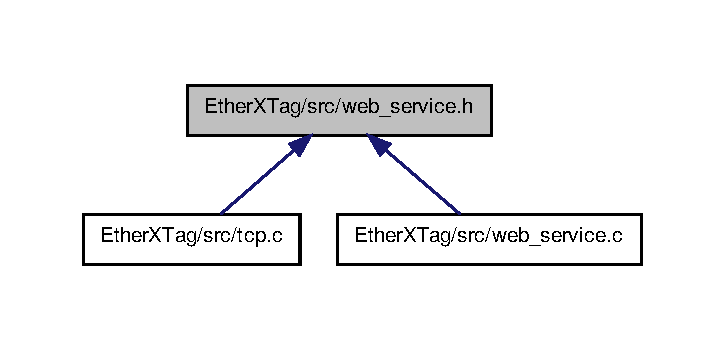
\includegraphics[width=348pt]{web__service_8h__dep__incl}
\end{center}
\end{figure}
\subsection*{Data Structures}
\begin{DoxyCompactItemize}
\item 
struct \hyperlink{structpage__t}{page\-\_\-t}
\end{DoxyCompactItemize}
\subsection*{Typedefs}
\begin{DoxyCompactItemize}
\item 
typedef struct \hyperlink{structpage__t}{page\-\_\-t} \hyperlink{web__service_8h_a578f79a5577c5f6a86cae8e9936ffa22}{page\-\_\-t}
\end{DoxyCompactItemize}
\subsection*{Functions}
\begin{DoxyCompactItemize}
\item 
\hyperlink{structpage__t}{page\-\_\-t} $\ast$ \hyperlink{web__service_8h_a5a94d9ecf7963c0150225d8acb17f6ea}{get\-Page} ()
\item 
const char $\ast$ \hyperlink{web__service_8h_a57eb4e125f533b812f7153767d315d1e}{get\-H\-T\-T\-P\-Header} ()
\item 
const char $\ast$ \hyperlink{web__service_8h_aba6e8228ddb103ef147d1108503f46e2}{get\-Page\-Content} ()
\end{DoxyCompactItemize}


\subsection{Typedef Documentation}
\hypertarget{web__service_8h_a578f79a5577c5f6a86cae8e9936ffa22}{\index{web\-\_\-service.\-h@{web\-\_\-service.\-h}!page\-\_\-t@{page\-\_\-t}}
\index{page\-\_\-t@{page\-\_\-t}!web_service.h@{web\-\_\-service.\-h}}
\subsubsection[{page\-\_\-t}]{\setlength{\rightskip}{0pt plus 5cm}typedef struct {\bf page\-\_\-t}  {\bf page\-\_\-t}}}\label{web__service_8h_a578f79a5577c5f6a86cae8e9936ffa22}


\subsection{Function Documentation}
\hypertarget{web__service_8h_a57eb4e125f533b812f7153767d315d1e}{\index{web\-\_\-service.\-h@{web\-\_\-service.\-h}!get\-H\-T\-T\-P\-Header@{get\-H\-T\-T\-P\-Header}}
\index{get\-H\-T\-T\-P\-Header@{get\-H\-T\-T\-P\-Header}!web_service.h@{web\-\_\-service.\-h}}
\subsubsection[{get\-H\-T\-T\-P\-Header}]{\setlength{\rightskip}{0pt plus 5cm}const char$\ast$ get\-H\-T\-T\-P\-Header (
\begin{DoxyParamCaption}
{}
\end{DoxyParamCaption}
)}}\label{web__service_8h_a57eb4e125f533b812f7153767d315d1e}


Definition at line 23 of file web\-\_\-service.\-c.

\hypertarget{web__service_8h_a5a94d9ecf7963c0150225d8acb17f6ea}{\index{web\-\_\-service.\-h@{web\-\_\-service.\-h}!get\-Page@{get\-Page}}
\index{get\-Page@{get\-Page}!web_service.h@{web\-\_\-service.\-h}}
\subsubsection[{get\-Page}]{\setlength{\rightskip}{0pt plus 5cm}{\bf page\-\_\-t}$\ast$ get\-Page (
\begin{DoxyParamCaption}
{}
\end{DoxyParamCaption}
)}}\label{web__service_8h_a5a94d9ecf7963c0150225d8acb17f6ea}


Definition at line 6 of file web\-\_\-service.\-c.

\hypertarget{web__service_8h_aba6e8228ddb103ef147d1108503f46e2}{\index{web\-\_\-service.\-h@{web\-\_\-service.\-h}!get\-Page\-Content@{get\-Page\-Content}}
\index{get\-Page\-Content@{get\-Page\-Content}!web_service.h@{web\-\_\-service.\-h}}
\subsubsection[{get\-Page\-Content}]{\setlength{\rightskip}{0pt plus 5cm}const char$\ast$ get\-Page\-Content (
\begin{DoxyParamCaption}
{}
\end{DoxyParamCaption}
)}}\label{web__service_8h_aba6e8228ddb103ef147d1108503f46e2}


Definition at line 27 of file web\-\_\-service.\-c.


\printindex
\end{document}
